\documentclass[letterpaper]{article}
\usepackage{makeidx}
\usepackage{graphicx}
\usepackage{multicol}
\usepackage{float}
\usepackage{listings}
\usepackage{color}
\usepackage{ifthen}
\usepackage[table]{xcolor}
\usepackage{textcomp}
\usepackage{alltt}
\usepackage{ifpdf}
\ifpdf
\usepackage[pdftex,
            pagebackref=true,
            colorlinks=true,
            linkcolor=blue,
            unicode
           ]{hyperref}
\else
\usepackage[ps2pdf,
            pagebackref=true,
            colorlinks=true,
            linkcolor=blue,
            unicode
           ]{hyperref}
\usepackage{pspicture}
\fi
\usepackage[utf8]{inputenc}
\usepackage{mathptmx}
\usepackage[scaled=.90]{helvet}
\usepackage{courier}
\usepackage{sectsty}
\usepackage[titles]{tocloft}
\usepackage{doxygen}
\lstset{language=C++,inputencoding=utf8,basicstyle=\footnotesize,breaklines=true,breakatwhitespace=true,tabsize=8,numbers=left }
\makeindex
\setcounter{tocdepth}{3}
\renewcommand{\footrulewidth}{0.4pt}
\renewcommand{\familydefault}{\sfdefault}
\begin{document}
\hypersetup{pageanchor=false}
\begin{titlepage}
\vspace*{7cm}
\begin{center}
{\Large wuparam \\[1ex]\large 0.1 }\\
\vspace*{1cm}
{\large Generated by Doxygen 1.7.4}\\
\vspace*{0.5cm}
{\small Tue Nov 1 2011 18:52:49}\\
\end{center}
\end{titlepage}
\pagenumbering{roman}
\tableofcontents
\pagenumbering{arabic}
\hypersetup{pageanchor=true}
\section{wuparam -\/ WU Whipple Data Analysis Package}
\label{index}\hypertarget{index}{}wuparam calculates the Hillas Parameters for events stored in Whipple telescope raw data files. -\/ To compile and run wuparam, you must install the following packages:
\begin{DoxyEnumerate}
\item The GNU Scientific Library (GSL) (\href{http://rpmfind.net/linux/rpm2html/search.php?query=gsl-devel}{\tt http://rpmfind.net/linux/rpm2html/search.php?query=gsl-\/devel})
\item GNU plotutils package (\href{http://rpmfind.net/linux/rpm2html/search.php?query=plotutils}{\tt http://rpmfind.net/linux/rpm2html/search.php?query=plotutils}) 
\end{DoxyEnumerate}
\section{Todo List}
\label{todo}
\hypertarget{todo}{}
\label{todo__todo000011}
\hypertarget{todo__todo000011}{}
 
\begin{DoxyDescription}
\item[Class \hyperlink{classAnalysisException}{AnalysisException} ]: \hyperlink{classAnalysisException}{AnalysisException} should be a subclass of the STL exception 
\end{DoxyDescription}

\label{todo__todo000001}
\hypertarget{todo__todo000001}{}
 
\begin{DoxyDescription}
\item[Class \hyperlink{classCamera}{Camera} ]: make separate classes for each camera 
\end{DoxyDescription}

\label{todo__todo000006}
\hypertarget{todo__todo000006}{}
 
\begin{DoxyDescription}
\item[Class \hyperlink{classCutter}{Cutter} ]: this is a badly designed class. \hyperlink{classCutter}{Cutter} should be a small object which applies a specific set of cuts (subclasses for other cutting methods). All the analysis should be done elsewhere.

: For multi-\/telescope analysis, make a telescope\_\-id argument or field and only process events from the specified telescope. 
\end{DoxyDescription}

\label{todo__todo000004}
\hypertarget{todo__todo000004}{}
 
\begin{DoxyDescription}
\item[Member \hyperlink{classCutter_a5c8d71e05e508ec60db78436b4ba416d}{Cutter::cut}(\hyperlink{classRunInfo}{RunInfo} \&, const std::string \&, char) ]: Implement 2-\/D analysis for tracking runs (currently, only ON/OFF pairs are used.

: separate total alpha plot for tracking runs.
\end{DoxyDescription}

\label{todo__todo000012}
\hypertarget{todo__todo000012}{}
 
\begin{DoxyDescription}
\item[Member \hyperlink{classEZCutter_adfef095f257966676350821591df66ed}{EZCutter::applyCorrections}(\hyperlink{structHillasParameterization}{HillasParameterization} \&p) ]: make sigma\_\-pix and the \char`\"{}0.023\char`\"{} free optimization parameters! 
\end{DoxyDescription}

\label{todo__todo000015}
\hypertarget{todo__todo000015}{}
 
\begin{DoxyDescription}
\item[Member \hyperlink{classFitter_a88492ebdbfa181370dc05a584ec9a040}{Fitter::minimize}(\hyperlink{classEnergySpectrum}{EnergySpectrum} $\ast$energy\_\-on, \hyperlink{classEnergySpectrum}{EnergySpectrum} $\ast$energy\_\-off, double \&N0, double \&Gamma0, double \&e0, double Time, double n0Range, int n0Step, double gRange, int gStep, double onoffratio) ]: put \char`\"{}alpha\char`\"{} or tracking ratio into the onOff and onOffVariance: onoff = on-\/a$\ast$off, variance=a$\ast$(on+off) or whatever
\end{DoxyDescription}

\label{todo__todo000018}
\hypertarget{todo__todo000018}{}
 
\begin{DoxyDescription}
\item[Member \hyperlink{classFitter_a6f93aeb7b89a67f368cfa03abdce3e5a}{Fitter::minimize}(\hyperlink{classEnergySpectrum}{EnergySpectrum} $\ast$energy\_\-on, \hyperlink{classEnergySpectrum}{EnergySpectrum} $\ast$energy\_\-off, double \&N0, double \&Gamma0, double \&E0, double Time, double n0Range, int n0Step, double gRange, int gStep, double e0Range, double e0Step, double onoffratio) ]: put \char`\"{}alpha\char`\"{} or tracking ratio into the onOff and onOffVariance: onoff = on-\/a$\ast$off, variance=a$\ast$(on+off) or whatever
\end{DoxyDescription}

\label{todo__todo000019}
\hypertarget{todo__todo000019}{}
 
\begin{DoxyDescription}
\item[Member \hyperlink{classGainFinder_a093922ed07e211199e2e3afdc4b6b2d4}{GainFinder::getGains}(\hyperlink{classRunInfo}{RunInfo} \&ri, Array\_\-t \&gains, int telescope\_\-id=0) ]: make gains database have a code column which marks bad gains 

: implement lock file! 
\end{DoxyDescription}

\label{todo__todo000010}
\hypertarget{todo__todo000010}{}
 
\begin{DoxyDescription}
\item[Class \hyperlink{structHeaderRecord}{HeaderRecord} ]: add fields for picture/boundary threshold so they can be checked by wucut -\/ don't want to accidently use cuts which were designed for one threshold after you parameterize with another! 
\end{DoxyDescription}

\label{todo__todo000020}
\hypertarget{todo__todo000020}{}
 
\begin{DoxyDescription}
\item[Class \hyperlink{classHistogram}{Histogram} ]: Make this class work with lightcurve data where the first and last bins may be partially filled (or smaller width) 
\end{DoxyDescription}

\label{todo__todo000021}
\hypertarget{todo__todo000021}{}
 
\begin{DoxyDescription}
\item[Member \hyperlink{classImage2D_afa47c6e966ae69c72bb58e97f1e58858}{Image2D::addHistRadially}(double x, double y, double val, float radius) ]: can speed this up considerably with geometric considerations (by only iterating over range of pixels that fall withing radius$\ast$2 for example) 
\end{DoxyDescription}

\label{todo__todo000013}
\hypertarget{todo__todo000013}{}
 
\begin{DoxyDescription}
\item[Member \hyperlink{classMCSpectrum_ae7bb310b53fe6faf2fbdb74017c627db}{MCSpectrum::MCSpectrum}(\hyperlink{classRunInfo}{RunInfo} \&ri) ]: make the specific energy estimator function user selectable (LZA vs small zenith, etc.) 

: make the specific energy estimator function user selectable (LZA vs small zenith, etc.) 
\end{DoxyDescription}

\label{todo__todo000023}
\hypertarget{todo__todo000023}{}
 
\begin{DoxyDescription}
\item[Member \hyperlink{classParamDataReader_a6c08000e4e3d408ae14b3146145a1249}{ParamDataReader::getHeaderRecord}(\hyperlink{structHeaderRecord}{HeaderRecord} \&hdr) ]: should make a ParamHeaderRecord which is a subclass of \hyperlink{structHeaderRecord}{HeaderRecord} which has all the extra parameterized info (like whether zcuts was enabled, etc.) 
\end{DoxyDescription}

\label{todo__todo000028}
\hypertarget{todo__todo000028}{}
 
\begin{DoxyDescription}
\item[Member \hyperlink{classPedestalFinder_a2f74e3e8ba1b0531f69949adb46d0657}{PedestalFinder::getPeds}(\hyperlink{classRunInfo}{RunInfo} \&ri, const std::string \&id, std::vector$<$ Pedestal $>$ \&, int telescope\_\-id=0) ]: Simulations only contain one pedestal record, so their dispersions are always 0. Due to this, the \hyperlink{classImageCleaner}{ImageCleaner} accepts too many pixels, since it uses the picthresh$\ast$peddisp as the threshold! Need to fix somehow...

: implement lockfiles to prevent more than one process from writing/reading to the database (necessary for the MPI-\/enabled or a multi-\/threaded version) 
\end{DoxyDescription}

\label{todo__todo000030}
\hypertarget{todo__todo000030}{}
 
\begin{DoxyDescription}
\item[Member \hyperlink{classPlotMaker_a7a63b2f17f113ee6b880aebf1cba1d91}{PlotMaker::plotAxes}() ]: don't plot minor tics where a major tic is 
\end{DoxyDescription}

\label{todo__todo000008}
\hypertarget{todo__todo000008}{}
 
\begin{DoxyDescription}
\item[Member \hyperlink{classRawDataReaderSim_acd4f407d9c8b8df95eb88213e6625f5f}{RawDataReaderSim::getHeaderRecord}(\hyperlink{structRawHeaderRecord}{RawHeaderRecord} \&header) ]: fill in the correct values 
\end{DoxyDescription}

\label{todo__todo000009}
\hypertarget{todo__todo000009}{}
 
\begin{DoxyDescription}
\item[Member \hyperlink{classRawDataReaderVText_a7fb3e50fa41df971c06c1b424c713675}{RawDataReaderVText::getHeaderRecord}(\hyperlink{structRawHeaderRecord}{RawHeaderRecord} \&header) ]: fill in the correct values 
\end{DoxyDescription}

\label{todo__todo000002}
\hypertarget{todo__todo000002}{}
 
\begin{DoxyDescription}
\item[Class \hyperlink{classRunInfo}{RunInfo} ]: Make \hyperlink{classRunInfo}{RunInfo} serializable so it can be sent as an MPI message?

: Make \hyperlink{classRunInfo}{RunInfo} saveable (i.e. write out a config file containing all the settings. This can be written to each run output dir so you can check what settings were used at the last parameterization. You can then use a \hyperlink{classConfig}{Config} object to parse the saved settings and check if the \hyperlink{classRunInfo}{RunInfo} has changed as a robust check for reparameterizing. Save() load() compare()
\end{DoxyDescription}

\label{todo__todo000031}
\hypertarget{todo__todo000031}{}
 
\begin{DoxyDescription}
\item[Member \hyperlink{classStarCatalog_a067a6b3ebbeed3d8c1450cc7092a9f64}{StarCatalog::findNearbyStars}(double, double, double, std::list$<$ Star $>$ \&) ]: check that this ra and dec from the tracking computer are already precessed, or from j2000 or something. If not already precessed, they need to be. 
\end{DoxyDescription}

\label{todo__todo000032}
\hypertarget{todo__todo000032}{}
 
\begin{DoxyDescription}
\item[Member \hyperlink{classStarCatalog_a7b487603d9556b01164515e8fb5fddd9}{StarCatalog::precessToDate}(int utdate) ]: Should check this -\/ it looks like stars are moving too much over the course of a year or so, so it's possible this is not working exactly right. However, it's pretty close. 
\end{DoxyDescription}

\label{todo__todo000033}
\hypertarget{todo__todo000033}{}
 
\begin{DoxyDescription}
\item[Member \hyperlink{classSuperCutter_a10e29b1d569a2b09755e44c31b3c1e61}{SuperCutter::pass}(\hyperlink{structHillasParameterization}{HillasParameterization} \&param, int cutmask) ]: right now, prePass occurs every time a cut is specified. That means it gets redone several times for each event! This shuold be done more efficiently without making it more confusing. 
\end{DoxyDescription}

\label{todo__todo000035}
\hypertarget{todo__todo000035}{}
 
\begin{DoxyDescription}
\item[Member \hyperlink{classZCutter_ad8fc95579fc4b47a518b66e6ea029f61}{ZCutter::applyCorrections}(\hyperlink{structHillasParameterization}{HillasParameterization} \&p) ]: make sigma\_\-pix and the \char`\"{}0.023\char`\"{} free optimization parameters! 
\end{DoxyDescription}
\section{Bug List}
\label{bug}
\hypertarget{bug}{}
\label{bug__bug000002}
\hypertarget{bug__bug000002}{}
 
\begin{DoxyDescription}
\item[Member \hyperlink{classHistogram_a57bd7d0018ca67ebc964a70856a45121}{Histogram::Histogram}(const \hyperlink{classHistogram}{Histogram} \&h) ]: doesn't work yet 
\end{DoxyDescription}

\label{bug__bug000001}
\hypertarget{bug__bug000001}{}
 
\begin{DoxyDescription}
\item[Member \hyperlink{classRawDataReaderSim_a3b39f633634f97e2962f80f2c60bf8b0}{RawDataReaderSim::RawDataReaderSim}(const std::string \&filename) ]: if file doesn't exist, doesn't always fail! 
\end{DoxyDescription}
\section{Namespace Index}
\subsection{Namespace List}
Here is a list of all documented namespaces with brief descriptions:\begin{DoxyCompactList}
\item\contentsline{section}{\hyperlink{namespaceCuts}{Cuts} (Contains enumerations for \hyperlink{classSuperCutter}{SuperCutter} and related cut objects )}{\pageref{namespaceCuts}}{}
\item\contentsline{section}{\hyperlink{namespaceWUArray}{WUArray} (Function prototypes and globals for wuarray )}{\pageref{namespaceWUArray}}{}
\end{DoxyCompactList}

\section{Class Index}
\subsection{Class Hierarchy}
This inheritance list is sorted roughly, but not completely, alphabetically:\begin{DoxyCompactList}
\item \contentsline{section}{AnalysisException}{\pageref{classAnalysisException}}{}
\begin{DoxyCompactList}
\item \contentsline{section}{CriticalAnalysisException}{\pageref{classCriticalAnalysisException}}{}
\item \contentsline{section}{MildAnalysisException}{\pageref{classMildAnalysisException}}{}
\begin{DoxyCompactList}
\item \contentsline{section}{EOFException}{\pageref{classEOFException}}{}
\item \contentsline{section}{RangeException}{\pageref{classRangeException}}{}
\end{DoxyCompactList}
\end{DoxyCompactList}
\item \contentsline{section}{Camera}{\pageref{classCamera}}{}
\item \contentsline{section}{Config}{\pageref{classConfig}}{}
\item \contentsline{section}{ContourSegment}{\pageref{structContourSegment}}{}
\item \contentsline{section}{Coordinate\_\-t}{\pageref{structCoordinate__t}}{}
\item \contentsline{section}{Cut}{\pageref{structCut}}{}
\item \contentsline{section}{CutFactory}{\pageref{classCutFactory}}{}
\item \contentsline{section}{CutInfo}{\pageref{structCutInfo}}{}
\item \contentsline{section}{Cutter}{\pageref{classCutter}}{}
\item \contentsline{section}{Data}{\pageref{structData}}{}
\item \contentsline{section}{DataReader}{\pageref{classDataReader}}{}
\begin{DoxyCompactList}
\item \contentsline{section}{ParamDataReader}{\pageref{classParamDataReader}}{}
\item \contentsline{section}{RawDataReader}{\pageref{classRawDataReader}}{}
\begin{DoxyCompactList}
\item \contentsline{section}{RawDataReaderHDF4}{\pageref{classRawDataReaderHDF4}}{}
\item \contentsline{section}{RawDataReaderSim}{\pageref{classRawDataReaderSim}}{}
\item \contentsline{section}{RawDataReaderVText}{\pageref{classRawDataReaderVText}}{}
\end{DoxyCompactList}
\end{DoxyCompactList}
\item \contentsline{section}{DataWriter}{\pageref{classDataWriter}}{}
\begin{DoxyCompactList}
\item \contentsline{section}{ParamDataWriter}{\pageref{classParamDataWriter}}{}
\begin{DoxyCompactList}
\item \contentsline{section}{ParamDataWriterNtuple}{\pageref{classParamDataWriterNtuple}}{}
\item \contentsline{section}{ParamDataWriterText}{\pageref{classParamDataWriterText}}{}
\end{DoxyCompactList}
\end{DoxyCompactList}
\item \contentsline{section}{EnergyEstimator}{\pageref{structEnergyEstimator}}{}
\begin{DoxyCompactList}
\item \contentsline{section}{LZAEnergyEstimator}{\pageref{structLZAEnergyEstimator}}{}
\item \contentsline{section}{SZAEnergyEstimator}{\pageref{structSZAEnergyEstimator}}{}
\item \contentsline{section}{Z40EnergyEstimator}{\pageref{structZ40EnergyEstimator}}{}
\item \contentsline{section}{Z50EnergyEstimator}{\pageref{structZ50EnergyEstimator}}{}
\end{DoxyCompactList}
\item \contentsline{section}{EnergyEstimatorFactory}{\pageref{classEnergyEstimatorFactory}}{}
\item \contentsline{section}{Fitter}{\pageref{classFitter}}{}
\item \contentsline{section}{GainFinder}{\pageref{classGainFinder}}{}
\item \contentsline{section}{GaussianDeviate}{\pageref{classGaussianDeviate}}{}
\item \contentsline{section}{Histogram}{\pageref{classHistogram}}{}
\begin{DoxyCompactList}
\item \contentsline{section}{EnergySpectrum}{\pageref{classEnergySpectrum}}{}
\end{DoxyCompactList}
\item \contentsline{section}{Image2D}{\pageref{classImage2D}}{}
\item \contentsline{section}{ImageAnalyzer}{\pageref{classImageAnalyzer}}{}
\begin{DoxyCompactList}
\item \contentsline{section}{HillasImageAnalyzer}{\pageref{classHillasImageAnalyzer}}{}
\item \contentsline{section}{MuonImageAnalyzer}{\pageref{classMuonImageAnalyzer}}{}
\end{DoxyCompactList}
\item \contentsline{section}{ImageCleaner}{\pageref{classImageCleaner}}{}
\begin{DoxyCompactList}
\item \contentsline{section}{DefaultImageCleaner}{\pageref{classDefaultImageCleaner}}{}
\item \contentsline{section}{ThresholdImageCleaner}{\pageref{classThresholdImageCleaner}}{}
\end{DoxyCompactList}
\item \contentsline{section}{ImageParameterization}{\pageref{structImageParameterization}}{}
\begin{DoxyCompactList}
\item \contentsline{section}{HillasParameterization}{\pageref{structHillasParameterization}}{}
\item \contentsline{section}{MuonParameterization}{\pageref{structMuonParameterization}}{}
\end{DoxyCompactList}
\item \contentsline{section}{Logger}{\pageref{classLogger}}{}
\item \contentsline{section}{MCBinInfo}{\pageref{structMCBinInfo}}{}
\item \contentsline{section}{MCRecord}{\pageref{structMCRecord}}{}
\item \contentsline{section}{MCSpectrum}{\pageref{classMCSpectrum}}{}
\item \contentsline{section}{Option\_\-s}{\pageref{structOption__s}}{}
\item \contentsline{section}{Parameterizer}{\pageref{classParameterizer}}{}
\item \contentsline{section}{ParseException}{\pageref{classParseException}}{}
\item \contentsline{section}{Pedestal}{\pageref{structPedestal}}{}
\item \contentsline{section}{PedestalFinder}{\pageref{classPedestalFinder}}{}
\item \contentsline{section}{PlotMaker}{\pageref{classPlotMaker}}{}
\item \contentsline{section}{ProgressBar}{\pageref{classProgressBar}}{}
\item \contentsline{section}{RawDataReaderFactory}{\pageref{classRawDataReaderFactory}}{}
\item \contentsline{section}{RawRunInfo}{\pageref{classRawRunInfo}}{}
\begin{DoxyCompactList}
\item \contentsline{section}{ParamRunInfo}{\pageref{classParamRunInfo}}{}
\begin{DoxyCompactList}
\item \contentsline{section}{CutRunInfo}{\pageref{classCutRunInfo}}{}
\end{DoxyCompactList}
\end{DoxyCompactList}
\item \contentsline{section}{Record}{\pageref{structRecord}}{}
\begin{DoxyCompactList}
\item \contentsline{section}{CutRecord}{\pageref{structCutRecord}}{}
\item \contentsline{section}{EventRecord}{\pageref{structEventRecord}}{}
\begin{DoxyCompactList}
\item \contentsline{section}{RawEventRecord}{\pageref{structRawEventRecord}}{}
\end{DoxyCompactList}
\item \contentsline{section}{HeaderRecord}{\pageref{structHeaderRecord}}{}
\begin{DoxyCompactList}
\item \contentsline{section}{RawHeaderRecord}{\pageref{structRawHeaderRecord}}{}
\end{DoxyCompactList}
\end{DoxyCompactList}
\item \contentsline{section}{Results}{\pageref{structResults}}{}
\item \contentsline{section}{RunInfo}{\pageref{classRunInfo}}{}
\begin{DoxyCompactList}
\item \contentsline{section}{PairRunInfo}{\pageref{classPairRunInfo}}{}
\item \contentsline{section}{TrackingRunInfo}{\pageref{classTrackingRunInfo}}{}
\end{DoxyCompactList}
\item \contentsline{section}{RunStatistics}{\pageref{structRunStatistics}}{}
\item \contentsline{section}{SimShowerRecord}{\pageref{structSimShowerRecord}}{}
\item \contentsline{section}{Star}{\pageref{classStar}}{}
\item \contentsline{section}{StarCatalog}{\pageref{classStarCatalog}}{}
\item \contentsline{section}{SuperCutter}{\pageref{classSuperCutter}}{}
\begin{DoxyCompactList}
\item \contentsline{section}{EZCutter}{\pageref{classEZCutter}}{}
\item \contentsline{section}{SpectralCutter}{\pageref{classSpectralCutter}}{}
\item \contentsline{section}{ZCutter}{\pageref{classZCutter}}{}
\end{DoxyCompactList}
\item \contentsline{section}{TelescopeArray}{\pageref{classTelescopeArray}}{}
\item \contentsline{section}{TelescopeArray::TelInfo}{\pageref{structTelescopeArray_1_1TelInfo}}{}
\end{DoxyCompactList}

\section{Class Index}
\subsection{Class List}
Here are the classes, structs, unions and interfaces with brief descriptions:\begin{DoxyCompactList}
\item\contentsline{section}{\hyperlink{classAnalysisException}{AnalysisException} (Standard exception thrown by analysis routines )}{\pageref{classAnalysisException}}{}
\item\contentsline{section}{\hyperlink{classCamera}{Camera} (Contains all operations pertaining to camera data )}{\pageref{classCamera}}{}
\item\contentsline{section}{\hyperlink{classConfig}{Config} (Loads Analysis configuration information from a text file )}{\pageref{classConfig}}{}
\item\contentsline{section}{\hyperlink{structContourSegment}{ContourSegment} }{\pageref{structContourSegment}}{}
\item\contentsline{section}{\hyperlink{structCoordinate__t}{Coordinate\_\-t} (A 2-\/d coordinate )}{\pageref{structCoordinate__t}}{}
\item\contentsline{section}{\hyperlink{classCriticalAnalysisException}{CriticalAnalysisException} (Thrown on errors in the analysis where the program cannot recover )}{\pageref{classCriticalAnalysisException}}{}
\item\contentsline{section}{\hyperlink{structCut}{Cut} (Describes range of values of a parameter to retain after cuts )}{\pageref{structCut}}{}
\item\contentsline{section}{\hyperlink{classCutFactory}{CutFactory} (Responsible for locating files and creating the correct data reader object for the detected file type )}{\pageref{classCutFactory}}{}
\item\contentsline{section}{\hyperlink{structCutInfo}{CutInfo} (Describes which cuts should be applied to the data )}{\pageref{structCutInfo}}{}
\item\contentsline{section}{\hyperlink{structCutRecord}{CutRecord} (Output from \hyperlink{classCutter}{Cutter} for each run.. )}{\pageref{structCutRecord}}{}
\item\contentsline{section}{\hyperlink{classCutRunInfo}{CutRunInfo} (\hyperlink{classParamRunInfo}{ParamRunInfo} + cut information )}{\pageref{classCutRunInfo}}{}
\item\contentsline{section}{\hyperlink{classCutter}{Cutter} (\hyperlink{namespaceCuts}{Cuts} parameterized data, calculates statistics, and generates final histograms )}{\pageref{classCutter}}{}
\item\contentsline{section}{\hyperlink{structData}{Data} (We store the data in an Array, We only want to know the number of excess counts, and the variance of this number )}{\pageref{structData}}{}
\item\contentsline{section}{\hyperlink{classDataReader}{DataReader} (Base class for all data readers (raw, parameterized, cut) )}{\pageref{classDataReader}}{}
\item\contentsline{section}{\hyperlink{classDataWriter}{DataWriter} (Base class for all data writers (parameterized data and cut data) )}{\pageref{classDataWriter}}{}
\item\contentsline{section}{\hyperlink{classDefaultImageCleaner}{DefaultImageCleaner} (The default cleaner uses a simple 2 threshold process )}{\pageref{classDefaultImageCleaner}}{}
\item\contentsline{section}{\hyperlink{structEnergyEstimator}{EnergyEstimator} }{\pageref{structEnergyEstimator}}{}
\item\contentsline{section}{\hyperlink{classEnergyEstimatorFactory}{EnergyEstimatorFactory} }{\pageref{classEnergyEstimatorFactory}}{}
\item\contentsline{section}{\hyperlink{classEnergySpectrum}{EnergySpectrum} (Energy Spectrum 1-\/D histogram class )}{\pageref{classEnergySpectrum}}{}
\item\contentsline{section}{\hyperlink{classEOFException}{EOFException} (Thrown by datareaders when the file is over )}{\pageref{classEOFException}}{}
\item\contentsline{section}{\hyperlink{structEventRecord}{EventRecord} (Event information )}{\pageref{structEventRecord}}{}
\item\contentsline{section}{\hyperlink{classEZCutter}{EZCutter} (Extended zenith cutterm Uses SuperCuts-\/like cuts, but with zenith angle corrections based on cos(theta) and 3rd order poly in log(SIZE) )}{\pageref{classEZCutter}}{}
\item\contentsline{section}{\hyperlink{classFitter}{Fitter} (Class that performs actual chi-\/square grid search )}{\pageref{classFitter}}{}
\item\contentsline{section}{\hyperlink{classGainFinder}{GainFinder} (Retrieve or calculate nitrogen gains, given a nitrogen run ID )}{\pageref{classGainFinder}}{}
\item\contentsline{section}{\hyperlink{classGaussianDeviate}{GaussianDeviate} }{\pageref{classGaussianDeviate}}{}
\item\contentsline{section}{\hyperlink{structHeaderRecord}{HeaderRecord} (Run information (header) from raw datafiles )}{\pageref{structHeaderRecord}}{}
\item\contentsline{section}{\hyperlink{classHillasImageAnalyzer}{HillasImageAnalyzer} (Calculates the Hillas parameters and 2D point of origin of a cleaned image )}{\pageref{classHillasImageAnalyzer}}{}
\item\contentsline{section}{\hyperlink{structHillasParameterization}{HillasParameterization} (Parameterization of an image, produced by the \hyperlink{classImageAnalyzer}{ImageAnalyzer} object )}{\pageref{structHillasParameterization}}{}
\item\contentsline{section}{\hyperlink{classHistogram}{Histogram} (General 1-\/D histogram class )}{\pageref{classHistogram}}{}
\item\contentsline{section}{\hyperlink{classImage2D}{Image2D} (Representation of a 2-\/D raster image (for 2D analysis) )}{\pageref{classImage2D}}{}
\item\contentsline{section}{\hyperlink{classImageAnalyzer}{ImageAnalyzer} (Base class for ImageAnalyzers -\/ components that look at an individual image and derive a set of parameters )}{\pageref{classImageAnalyzer}}{}
\item\contentsline{section}{\hyperlink{classImageCleaner}{ImageCleaner} (Abstract interface to all cleaning routines )}{\pageref{classImageCleaner}}{}
\item\contentsline{section}{\hyperlink{structImageParameterization}{ImageParameterization} (Information common to all parameterizations )}{\pageref{structImageParameterization}}{}
\item\contentsline{section}{\hyperlink{classLogger}{Logger} (Error log singleton )}{\pageref{classLogger}}{}
\item\contentsline{section}{\hyperlink{structLZAEnergyEstimator}{LZAEnergyEstimator} }{\pageref{structLZAEnergyEstimator}}{}
\item\contentsline{section}{\hyperlink{structMCBinInfo}{MCBinInfo} }{\pageref{structMCBinInfo}}{}
\item\contentsline{section}{\hyperlink{structMCRecord}{MCRecord} (For Each Monte Carlo Event That Passes the Selection \hyperlink{namespaceCuts}{Cuts}, We Want to Know the True Energy and the Reconstructed Energy )}{\pageref{structMCRecord}}{}
\item\contentsline{section}{\hyperlink{classMCSpectrum}{MCSpectrum} (Object that takes care of all the Monte Carlo (MC) dependent aspects: )}{\pageref{classMCSpectrum}}{}
\item\contentsline{section}{\hyperlink{classMildAnalysisException}{MildAnalysisException} (Thrown for warnings and recoverable errors )}{\pageref{classMildAnalysisException}}{}
\item\contentsline{section}{\hyperlink{classMuonImageAnalyzer}{MuonImageAnalyzer} (Analyzes the muon-\/like properties of an image )}{\pageref{classMuonImageAnalyzer}}{}
\item\contentsline{section}{\hyperlink{structMuonParameterization}{MuonParameterization} (Describes the muon-\/like characteristics of an image )}{\pageref{structMuonParameterization}}{}
\item\contentsline{section}{\hyperlink{structOption__s}{Option\_\-s} }{\pageref{structOption__s}}{}
\item\contentsline{section}{\hyperlink{classPairRunInfo}{PairRunInfo} }{\pageref{classPairRunInfo}}{}
\item\contentsline{section}{\hyperlink{classParamDataReader}{ParamDataReader} (Reads parameterized datafiles )}{\pageref{classParamDataReader}}{}
\item\contentsline{section}{\hyperlink{classParamDataWriter}{ParamDataWriter} (Base class for writing HillasParameterizations to disk )}{\pageref{classParamDataWriter}}{}
\item\contentsline{section}{\hyperlink{classParamDataWriterNtuple}{ParamDataWriterNtuple} (Outputs parameterized events to an N-\/Tuple (for use in for example, PAW) )}{\pageref{classParamDataWriterNtuple}}{}
\item\contentsline{section}{\hyperlink{classParamDataWriterText}{ParamDataWriterText} (Outputs parameterized events to a text file )}{\pageref{classParamDataWriterText}}{}
\item\contentsline{section}{\hyperlink{classParameterizer}{Parameterizer} (Contains all functions pretaining to the parameterization of raw data )}{\pageref{classParameterizer}}{}
\item\contentsline{section}{\hyperlink{classParamRunInfo}{ParamRunInfo} (Adds info calculated in the parameterize routine )}{\pageref{classParamRunInfo}}{}
\item\contentsline{section}{\hyperlink{classParseException}{ParseException} }{\pageref{classParseException}}{}
\item\contentsline{section}{\hyperlink{structPedestal}{Pedestal} (Contains information about the pedestal for a single tube )}{\pageref{structPedestal}}{}
\item\contentsline{section}{\hyperlink{classPedestalFinder}{PedestalFinder} (Class to generate pedestal values for a series of runs )}{\pageref{classPedestalFinder}}{}
\item\contentsline{section}{\hyperlink{classPlotMaker}{PlotMaker} (Plots stuff to any PlotUtils graphics context )}{\pageref{classPlotMaker}}{}
\item\contentsline{section}{\hyperlink{classProgressBar}{ProgressBar} (Displays a text-\/based progress bar with estimated time to finish for a particular task )}{\pageref{classProgressBar}}{}
\item\contentsline{section}{\hyperlink{classRangeException}{RangeException} (Thrown by datareaders when the file is over )}{\pageref{classRangeException}}{}
\item\contentsline{section}{\hyperlink{classRawDataReader}{RawDataReader} (Reads raw telescope data and produces coresponding records.. )}{\pageref{classRawDataReader}}{}
\item\contentsline{section}{\hyperlink{classRawDataReaderFactory}{RawDataReaderFactory} (Responsible for locating files and creating the correct data reader object for the detected file type )}{\pageref{classRawDataReaderFactory}}{}
\item\contentsline{section}{\hyperlink{classRawDataReaderHDF4}{RawDataReaderHDF4} (Implementation of \hyperlink{classRawDataReader}{RawDataReader} for HDF4 input files )}{\pageref{classRawDataReaderHDF4}}{}
\item\contentsline{section}{\hyperlink{classRawDataReaderSim}{RawDataReaderSim} (Implementation of \hyperlink{classRawDataReader}{RawDataReader} for simulation .tubes files )}{\pageref{classRawDataReaderSim}}{}
\item\contentsline{section}{\hyperlink{classRawDataReaderVText}{RawDataReaderVText} (Implementation of \hyperlink{classRawDataReader}{RawDataReader} VERITAS text data as outputed by Paul Rebillot's charge integration routines )}{\pageref{classRawDataReaderVText}}{}
\item\contentsline{section}{\hyperlink{structRawEventRecord}{RawEventRecord} (One event from a raw data file )}{\pageref{structRawEventRecord}}{}
\item\contentsline{section}{\hyperlink{structRawHeaderRecord}{RawHeaderRecord} }{\pageref{structRawHeaderRecord}}{}
\item\contentsline{section}{\hyperlink{classRawRunInfo}{RawRunInfo} (Header Information read from the raw data )}{\pageref{classRawRunInfo}}{}
\item\contentsline{section}{\hyperlink{structRecord}{Record} (Records are readable/writable (i.e )}{\pageref{structRecord}}{}
\item\contentsline{section}{\hyperlink{structResults}{Results} (Here We Store The \hyperlink{structResults}{Results} of the Chi-\/Square Fit )}{\pageref{structResults}}{}
\item\contentsline{section}{\hyperlink{classRunInfo}{RunInfo} (Basic structure returned by a \hyperlink{classConfig}{Config} object )}{\pageref{classRunInfo}}{}
\item\contentsline{section}{\hyperlink{structRunStatistics}{RunStatistics} }{\pageref{structRunStatistics}}{}
\item\contentsline{section}{\hyperlink{structSimShowerRecord}{SimShowerRecord} }{\pageref{structSimShowerRecord}}{}
\item\contentsline{section}{\hyperlink{classSpectralCutter}{SpectralCutter} (Implements cuts which scale with zenith angle and SIZE, otherwise very similar to SuperCuts )}{\pageref{classSpectralCutter}}{}
\item\contentsline{section}{\hyperlink{classStar}{Star} (Representation of a star )}{\pageref{classStar}}{}
\item\contentsline{section}{\hyperlink{classStarCatalog}{StarCatalog} (A searchable star database )}{\pageref{classStarCatalog}}{}
\item\contentsline{section}{\hyperlink{classSuperCutter}{SuperCutter} (Applies SuperCuts to a given \hyperlink{structHillasParameterization}{HillasParameterization} )}{\pageref{classSuperCutter}}{}
\item\contentsline{section}{\hyperlink{structSZAEnergyEstimator}{SZAEnergyEstimator} }{\pageref{structSZAEnergyEstimator}}{}
\item\contentsline{section}{\hyperlink{classTelescopeArray}{TelescopeArray} (Stores information for an array of telescopes, including \hyperlink{classCamera}{Camera} objects )}{\pageref{classTelescopeArray}}{}
\item\contentsline{section}{\hyperlink{structTelescopeArray_1_1TelInfo}{TelescopeArray::TelInfo} }{\pageref{structTelescopeArray_1_1TelInfo}}{}
\item\contentsline{section}{\hyperlink{classThresholdImageCleaner}{ThresholdImageCleaner} }{\pageref{classThresholdImageCleaner}}{}
\item\contentsline{section}{\hyperlink{classTrackingRunInfo}{TrackingRunInfo} }{\pageref{classTrackingRunInfo}}{}
\item\contentsline{section}{\hyperlink{structZ40EnergyEstimator}{Z40EnergyEstimator} }{\pageref{structZ40EnergyEstimator}}{}
\item\contentsline{section}{\hyperlink{structZ50EnergyEstimator}{Z50EnergyEstimator} }{\pageref{structZ50EnergyEstimator}}{}
\item\contentsline{section}{\hyperlink{classZCutter}{ZCutter} (Originial zenith cutter, from ZCuts99 )}{\pageref{classZCutter}}{}
\end{DoxyCompactList}

\section{Namespace Documentation}
\hypertarget{namespaceCuts}{
\subsection{Cuts Namespace Reference}
\label{namespaceCuts}\index{Cuts@{Cuts}}
}


Contains enumerations for \hyperlink{classSuperCutter}{SuperCutter} and related cut objects.  


\subsubsection*{Enumerations}
\begin{DoxyCompactItemize}
\item 
enum {\bfseries CutMask} \{ \par
{\bfseries SIZE} =  1 $<$$<$ 0, 
{\bfseries MAX} =  1 $<$$<$ 1, 
{\bfseries FRAC} =  1 $<$$<$ 2, 
{\bfseries LENSIZE} =  1 $<$$<$ 3, 
\par
{\bfseries DISTANCE} =  1 $<$$<$ 4, 
{\bfseries LENGTH} =  1 $<$$<$ 5, 
{\bfseries WIDTH} =  1 $<$$<$ 6, 
{\bfseries ALPHA} =  1 $<$$<$ 7, 
\par
{\bfseries ASYMM} =  1 $<$$<$ 8, 
{\bfseries ALL\_\-CUTS} =  0xFFFFFFFF
 \}
\end{DoxyCompactItemize}


\subsubsection{Detailed Description}
Contains enumerations for \hyperlink{classSuperCutter}{SuperCutter} and related cut objects. 
\hypertarget{namespaceWUArray}{
\subsection{WUArray Namespace Reference}
\label{namespaceWUArray}\index{WUArray@{WUArray}}
}


Function prototypes and globals for wuarray.  


\subsubsection*{Enumerations}
\begin{DoxyCompactItemize}
\item 
enum \hyperlink{namespaceWUArray_abd3f6c10cbcfe7fa4e24e4bce5522ab8}{RunType} \{ {\bfseries TRACK}, 
{\bfseries ON}, 
{\bfseries OFF}
 \}
\end{DoxyCompactItemize}
\subsubsection*{Functions}
\begin{DoxyCompactItemize}
\item 
\hypertarget{namespaceWUArray_ab642d5effbed86a60d236513ba68de8c}{
void \hyperlink{namespaceWUArray_ab642d5effbed86a60d236513ba68de8c}{showUsage} ()}
\label{namespaceWUArray_ab642d5effbed86a60d236513ba68de8c}

\item 
void \hyperlink{namespaceWUArray_a91ddbe526ff9aab8db00c8a40d09867c}{getCommandLineOptions} (int argc, char $\ast$$\ast$argv)
\item 
\hypertarget{namespaceWUArray_a69545c23f3068ab0280f3be54345a006}{
void {\bfseries shutdown} ()}
\label{namespaceWUArray_a69545c23f3068ab0280f3be54345a006}

\item 
\hypertarget{namespaceWUArray_ab448bf290a1eea9d1c5f8ecc9adbcccd}{
void {\bfseries trap\_\-ctrl\_\-c} (int)}
\label{namespaceWUArray_ab448bf290a1eea9d1c5f8ecc9adbcccd}

\item 
void \hyperlink{namespaceWUArray_a7ed5ef4b896abeb0025832e0b5a737bd}{process} (\hyperlink{classRunInfo}{RunInfo} \&ri)
\item 
void \hyperlink{namespaceWUArray_a257a781e9eccd9e0061a1d21afa9329d}{analyzeRun} (\hyperlink{classRunInfo}{RunInfo} \&ri, \hyperlink{namespaceWUArray_abd3f6c10cbcfe7fa4e24e4bce5522ab8}{RunType} runtype)
\end{DoxyCompactItemize}
\subsubsection*{Variables}
\begin{DoxyCompactItemize}
\item 
\hypertarget{namespaceWUArray_ae13800389922672d48647bdf1a8fb8cc}{
\hyperlink{classPlotMaker}{PlotMaker} $\ast$ {\bfseries pm} = NULL}
\label{namespaceWUArray_ae13800389922672d48647bdf1a8fb8cc}

\end{DoxyCompactItemize}


\subsubsection{Detailed Description}
Function prototypes and globals for wuarray. I put these in their own namespace so they don't conflict with functions in wuparam, wucut, etc. 

\subsubsection{Function Documentation}
\hypertarget{namespaceWUArray_a257a781e9eccd9e0061a1d21afa9329d}{
\index{WUArray@{WUArray}!analyzeRun@{analyzeRun}}
\index{analyzeRun@{analyzeRun}!WUArray@{WUArray}}
\paragraph[{analyzeRun}]{\setlength{\rightskip}{0pt plus 5cm}void WUArray::analyzeRun (
\begin{DoxyParamCaption}
\item[{{\bf RunInfo} \&}]{ri, }
\item[{{\bf WUArray::RunType}}]{runtype}
\end{DoxyParamCaption}
)}}
\label{namespaceWUArray_a257a781e9eccd9e0061a1d21afa9329d}


Analyze a single run. 

This is called by process. Right now, it just reads the data and demonstrates some simple things you can do.


\begin{DoxyParams}{Parameters}
{\em ri} & the full run-\/info struct \\
\hline
{\em runtype} & -\/ should be process the on, off, or tracking run? These cases may be treated separately. \\
\hline
\end{DoxyParams}


Definition at line 218 of file wuarray.cpp.



References Image2D::addHistRadially(), HillasParameterization::alpha, RunInfo::arrayconfig, ParamDataReader::getHeaderRecord(), Camera::getNumPixels(), Histogram::increment(), HeaderRecord::nadc, HeaderRecord::num\_\-telescopes, RunInfo::offid, RunInfo::onid, PlotMaker::plotAxes(), HillasParameterization::point\_\-of\_\-origin\_\-a, Image2D::save(), Image2D::setCoordinateBox(), HeaderRecord::sourcename, RunInfo::utdate, Coordinate\_\-t::x, and Coordinate\_\-t::y.



Referenced by process().

\hypertarget{namespaceWUArray_a91ddbe526ff9aab8db00c8a40d09867c}{
\index{WUArray@{WUArray}!getCommandLineOptions@{getCommandLineOptions}}
\index{getCommandLineOptions@{getCommandLineOptions}!WUArray@{WUArray}}
\paragraph[{getCommandLineOptions}]{\setlength{\rightskip}{0pt plus 5cm}void WUArray::getCommandLineOptions (
\begin{DoxyParamCaption}
\item[{int}]{argc, }
\item[{char $\ast$$\ast$}]{argv}
\end{DoxyParamCaption}
)}}
\label{namespaceWUArray_a91ddbe526ff9aab8db00c8a40d09867c}


This specifies and processes the various command-\/line options. 

See the getopt manpage for more information (type 'man 3 getopt' to see the C documentation, which is in manual section 3). 

Definition at line 421 of file wuarray.cpp.

\hypertarget{namespaceWUArray_a7ed5ef4b896abeb0025832e0b5a737bd}{
\index{WUArray@{WUArray}!process@{process}}
\index{process@{process}!WUArray@{WUArray}}
\paragraph[{process}]{\setlength{\rightskip}{0pt plus 5cm}void WUArray::process (
\begin{DoxyParamCaption}
\item[{{\bf RunInfo} \&}]{ri}
\end{DoxyParamCaption}
)}}
\label{namespaceWUArray_a7ed5ef4b896abeb0025832e0b5a737bd}


Process a single run. 

This is called for each run in the config file. 

Definition at line 182 of file wuarray.cpp.



References analyzeRun(), RunInfo::offid, RunInfo::onid, and RunInfo::type.


\section{Class Documentation}
\hypertarget{classAnalysisException}{
\subsection{AnalysisException Class Reference}
\label{classAnalysisException}\index{AnalysisException@{AnalysisException}}
}


Standard exception thrown by analysis routines.  




{\ttfamily \#include $<$Exceptions.h$>$}

Inheritance diagram for AnalysisException:\begin{figure}[H]
\begin{center}
\leavevmode
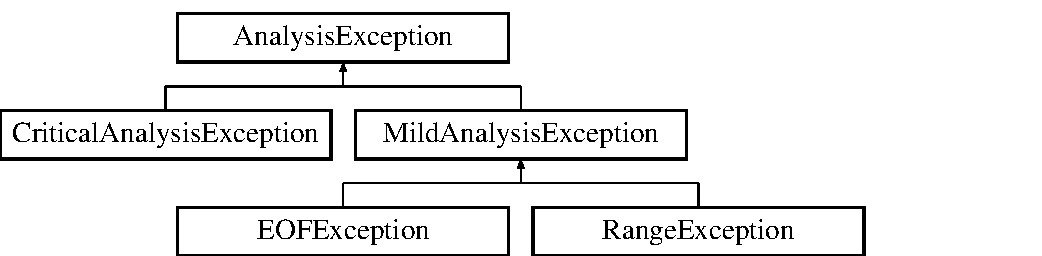
\includegraphics[height=3.000000cm]{classAnalysisException}
\end{center}
\end{figure}
\subsubsection*{Public Member Functions}
\begin{DoxyCompactItemize}
\item 
\hypertarget{classAnalysisException_a0ff1612d70c588e03de0b24744691a9f}{
{\bfseries AnalysisException} (std::string str)}
\label{classAnalysisException_a0ff1612d70c588e03de0b24744691a9f}

\end{DoxyCompactItemize}


\subsubsection{Detailed Description}
Standard exception thrown by analysis routines. 

\begin{Desc}
\item[\hyperlink{todo__todo000011}{Todo}]: \hyperlink{classAnalysisException}{AnalysisException} should be a subclass of the STL exception \end{Desc}


Definition at line 21 of file Exceptions.h.



The documentation for this class was generated from the following file:\begin{DoxyCompactItemize}
\item 
Exceptions.h\end{DoxyCompactItemize}

\hypertarget{classCamera}{
\subsection{Camera Class Reference}
\label{classCamera}\index{Camera@{Camera}}
}


Contains all operations pertaining to camera data.  




{\ttfamily \#include $<$Camera.h$>$}

\subsubsection*{Public Types}
\begin{DoxyCompactItemize}
\item 
enum {\bfseries CameraID} \{ \par
{\bfseries ID\_\-490}, 
{\bfseries ID\_\-331}, 
{\bfseries ID\_\-151}, 
{\bfseries ID\_\-109}, 
\par
{\bfseries ID\_\-V500}, 
{\bfseries ID\_\-UNKNOWN}
 \}
\end{DoxyCompactItemize}
\subsubsection*{Public Member Functions}
\begin{DoxyCompactItemize}
\item 
\hypertarget{classCamera_a797472a16ac17eeb0744ef09e56ba562}{
\hyperlink{classCamera_a797472a16ac17eeb0744ef09e56ba562}{Camera} (int npixels, Array\_\-t \&xcoords, Array\_\-t \&ycoords)}
\label{classCamera_a797472a16ac17eeb0744ef09e56ba562}

\item 
\hyperlink{classCamera_a0d7c5790cf94ea5e3ff670e39e037679}{Camera} (char $\ast$)
\item 
\hyperlink{classCamera_a2001776bff6855a02cddeed4706c004c}{Camera} (int npixels, int utdate=-\/1)
\item 
\hypertarget{classCamera_a0f575b530adf2e1d5e6c0ea51a22e219}{
void {\bfseries init} (char $\ast$)}
\label{classCamera_a0f575b530adf2e1d5e6c0ea51a22e219}

\item 
void \hyperlink{classCamera_a9b60c76986e0da3dd1a5f5764d718faa}{shiftCameraCoordinates} (double dx, double dy)
\item 
double \hyperlink{classCamera_a6e84df5ac1edf5b6bcfd44ddea17ee36}{getSigmaPSF} (double zen)
\item 
\hypertarget{classCamera_aa01bd8754f3f024237a094911c847798}{
double \hyperlink{classCamera_aa01bd8754f3f024237a094911c847798}{getSigmaPixel} ()}
\label{classCamera_aa01bd8754f3f024237a094911c847798}

\item 
\hypertarget{classCamera_a80e6c96d875b9d8145b87378beb41b9d}{
double \hyperlink{classCamera_a80e6c96d875b9d8145b87378beb41b9d}{getPEToDC} ()}
\label{classCamera_a80e6c96d875b9d8145b87378beb41b9d}

\item 
\hypertarget{classCamera_a4f2750f42d18cc49f5aa703466a64268}{
int \hyperlink{classCamera_a4f2750f42d18cc49f5aa703466a64268}{getNumPixels} ()}
\label{classCamera_a4f2750f42d18cc49f5aa703466a64268}

\item 
\hypertarget{classCamera_acd071e942d1e5403f7f8220f8c63edc4}{
int {\bfseries getFirstPixel} ()}
\label{classCamera_acd071e942d1e5403f7f8220f8c63edc4}

\item 
\hypertarget{classCamera_a233576d02d136e96d8886627c2512afc}{
int \hyperlink{classCamera_a233576d02d136e96d8886627c2512afc}{getLastPixel} ()}
\label{classCamera_a233576d02d136e96d8886627c2512afc}

\item 
int \hyperlink{classCamera_ac105d042bd3d5d7bad73ce3b2d8e7fb6}{getCameraID} ()
\item 
\hypertarget{classCamera_a8a4b74941bc6cfcd97ec1b135f6fec09}{
Array\_\-t \& \hyperlink{classCamera_a8a4b74941bc6cfcd97ec1b135f6fec09}{xCoords} ()}
\label{classCamera_a8a4b74941bc6cfcd97ec1b135f6fec09}

\item 
\hypertarget{classCamera_af2892e20c0a16ae802fcd8cc454bf59d}{
Array\_\-t \& \hyperlink{classCamera_af2892e20c0a16ae802fcd8cc454bf59d}{yCoords} ()}
\label{classCamera_af2892e20c0a16ae802fcd8cc454bf59d}

\item 
\hypertarget{classCamera_a6757b477302e1147fbcc5a5a6bb58122}{
Array\_\-t \& \hyperlink{classCamera_a6757b477302e1147fbcc5a5a6bb58122}{radii} ()}
\label{classCamera_a6757b477302e1147fbcc5a5a6bb58122}

\item 
\hypertarget{classCamera_a81881f3c5efe5c378457d825a719bcf8}{
double {\bfseries getMinX} ()}
\label{classCamera_a81881f3c5efe5c378457d825a719bcf8}

\item 
\hypertarget{classCamera_adc954eada08c2d7b9ce84860a9ccb77c}{
double {\bfseries getMinY} ()}
\label{classCamera_adc954eada08c2d7b9ce84860a9ccb77c}

\item 
\hypertarget{classCamera_a67522350c901f9143f60f7c0c31a4e37}{
double {\bfseries getMaxX} ()}
\label{classCamera_a67522350c901f9143f60f7c0c31a4e37}

\item 
\hypertarget{classCamera_a9a18da3683ade906048a58a110574fc4}{
double {\bfseries getMaxY} ()}
\label{classCamera_a9a18da3683ade906048a58a110574fc4}

\item 
\hypertarget{classCamera_a8c5b3c611d93f62e80d2de1dd9bef888}{
std::list$<$ int $>$ $\ast$ \hyperlink{classCamera_a8c5b3c611d93f62e80d2de1dd9bef888}{getNeighborListOfPixel} (int n)}
\label{classCamera_a8c5b3c611d93f62e80d2de1dd9bef888}

\end{DoxyCompactItemize}
\subsubsection*{Static Public Attributes}
\begin{DoxyCompactItemize}
\item 
\hypertarget{classCamera_ad4b47a9bd69e1f761922fefaa0f1ad10}{
static const int {\bfseries AUTOSCALE} = -\/1}
\label{classCamera_ad4b47a9bd69e1f761922fefaa0f1ad10}

\end{DoxyCompactItemize}


\subsubsection{Detailed Description}
Contains all operations pertaining to camera data. 

This includes loading the camera pixel positions from a file and building the pixel neighborlist.

\begin{Desc}
\item[\hyperlink{todo__todo000001}{Todo}]: make separate classes for each camera \end{Desc}


Definition at line 28 of file Camera.h.



\subsubsection{Constructor \& Destructor Documentation}
\hypertarget{classCamera_a0d7c5790cf94ea5e3ff670e39e037679}{
\index{Camera@{Camera}!Camera@{Camera}}
\index{Camera@{Camera}!Camera@{Camera}}
\paragraph[{Camera}]{\setlength{\rightskip}{0pt plus 5cm}Camera::Camera (
\begin{DoxyParamCaption}
\item[{char $\ast$}]{filename}
\end{DoxyParamCaption}
)}}
\label{classCamera_a0d7c5790cf94ea5e3ff670e39e037679}


Create a \hyperlink{classCamera}{Camera} object. 


\begin{DoxyParams}{Parameters}
{\em filename} & filename of the camera definition file. \\
\hline
\end{DoxyParams}


Definition at line 28 of file Camera.cpp.

\hypertarget{classCamera_a2001776bff6855a02cddeed4706c004c}{
\index{Camera@{Camera}!Camera@{Camera}}
\index{Camera@{Camera}!Camera@{Camera}}
\paragraph[{Camera}]{\setlength{\rightskip}{0pt plus 5cm}Camera::Camera (
\begin{DoxyParamCaption}
\item[{int}]{npixels, }
\item[{int}]{utdate = {\ttfamily -\/1}}
\end{DoxyParamCaption}
)}}
\label{classCamera_a2001776bff6855a02cddeed4706c004c}


PFR: change year switch to year+month switch. telescope seasons are fiscal-\/ they start in june of one year, and go until june of the next! This should only use one pe2dc ratio, but previously it used 2.



Definition at line 36 of file Camera.cpp.



\subsubsection{Member Function Documentation}
\hypertarget{classCamera_ac105d042bd3d5d7bad73ce3b2d8e7fb6}{
\index{Camera@{Camera}!getCameraID@{getCameraID}}
\index{getCameraID@{getCameraID}!Camera@{Camera}}
\paragraph[{getCameraID}]{\setlength{\rightskip}{0pt plus 5cm}int Camera::getCameraID (
\begin{DoxyParamCaption}
{}
\end{DoxyParamCaption}
)\hspace{0.3cm}{\ttfamily  \mbox{[}inline\mbox{]}}}}
\label{classCamera_ac105d042bd3d5d7bad73ce3b2d8e7fb6}


last pixel \# to use 

\hyperlink{classCamera}{Camera} ID number 

Definition at line 47 of file Camera.h.



Referenced by Parameterizer::printSummary().

\hypertarget{classCamera_a6e84df5ac1edf5b6bcfd44ddea17ee36}{
\index{Camera@{Camera}!getSigmaPSF@{getSigmaPSF}}
\index{getSigmaPSF@{getSigmaPSF}!Camera@{Camera}}
\paragraph[{getSigmaPSF}]{\setlength{\rightskip}{0pt plus 5cm}double Camera::getSigmaPSF (
\begin{DoxyParamCaption}
\item[{double}]{zen}
\end{DoxyParamCaption}
)}}
\label{classCamera_a6e84df5ac1edf5b6bcfd44ddea17ee36}


Point spread dispersion. 

Returns the estimated dispersion due to the point spread function of the camera at the given zenith angle. 

Definition at line 353 of file Camera.cpp.



Referenced by ZCutter::applyCorrections().

\hypertarget{classCamera_a9b60c76986e0da3dd1a5f5764d718faa}{
\index{Camera@{Camera}!shiftCameraCoordinates@{shiftCameraCoordinates}}
\index{shiftCameraCoordinates@{shiftCameraCoordinates}!Camera@{Camera}}
\paragraph[{shiftCameraCoordinates}]{\setlength{\rightskip}{0pt plus 5cm}void Camera::shiftCameraCoordinates (
\begin{DoxyParamCaption}
\item[{double}]{dx, }
\item[{double}]{dy}
\end{DoxyParamCaption}
)}}
\label{classCamera_a9b60c76986e0da3dd1a5f5764d718faa}


translate the camera coordinates by the specified amount. 

This is used to fix offsets in the camera due to telescope flexing at low elevation, for example. 

Definition at line 376 of file Camera.cpp.



The documentation for this class was generated from the following files:\begin{DoxyCompactItemize}
\item 
Camera.h\item 
Camera.cpp\end{DoxyCompactItemize}

\hypertarget{classConfig}{
\subsection{Config Class Reference}
\label{classConfig}\index{Config@{Config}}
}


Loads Analysis configuration information from a text file.  




{\ttfamily \#include $<$Config.h$>$}

\subsubsection*{Public Types}
\begin{DoxyCompactItemize}
\item 
enum {\bfseries RunType} \{ {\bfseries TRACK}, 
{\bfseries ONOFF}
 \}
\item 
enum {\bfseries OutType} \{ {\bfseries NTUPLE}, 
{\bfseries TEXT}
 \}
\item 
enum {\bfseries CutType} \{ {\bfseries SUPERCUTTER}, 
{\bfseries ZCUTTER}, 
{\bfseries EZCUTTER}, 
{\bfseries SPECTRALCUTTER}
 \}
\end{DoxyCompactItemize}
\subsubsection*{Public Member Functions}
\begin{DoxyCompactItemize}
\item 
\hypertarget{classConfig_a7107b9451a2c5e2d68b31c27b6767529}{
{\bfseries Config} (char $\ast$filename)}
\label{classConfig_a7107b9451a2c5e2d68b31c27b6767529}

\item 
\hypertarget{classConfig_a41d36d315f24a126e7f0d0506bc001e6}{
void \hyperlink{classConfig_a41d36d315f24a126e7f0d0506bc001e6}{writeSample} (char $\ast$file)}
\label{classConfig_a41d36d315f24a126e7f0d0506bc001e6}

\item 
\hypertarget{classConfig_ab4adb3c03021c77c13b07864e0c643c2}{
\hyperlink{classRunInfo}{RunInfo} \hyperlink{classConfig_ab4adb3c03021c77c13b07864e0c643c2}{getNextRun} ()}
\label{classConfig_ab4adb3c03021c77c13b07864e0c643c2}

\item 
\hypertarget{classConfig_a93688b97b30ef4c399f979187e1db014}{
std::deque$<$ \hyperlink{classRunInfo}{RunInfo} $>$ \& {\bfseries getRunQueue} ()}
\label{classConfig_a93688b97b30ef4c399f979187e1db014}

\item 
\hypertarget{classConfig_a217ba471f05a4b279a699505cec8160f}{
bool {\bfseries isDone} ()}
\label{classConfig_a217ba471f05a4b279a699505cec8160f}

\item 
\hypertarget{classConfig_aa3db1fe06efca6585599321d61020fa3}{
int {\bfseries getRunCount} ()}
\label{classConfig_aa3db1fe06efca6585599321d61020fa3}

\end{DoxyCompactItemize}


\subsubsection{Detailed Description}
Loads Analysis configuration information from a text file. 

Definition at line 191 of file Config.h.



The documentation for this class was generated from the following files:\begin{DoxyCompactItemize}
\item 
Config.h\item 
Config.cpp\end{DoxyCompactItemize}

\hypertarget{structContourSegment}{
\subsection{ContourSegment Struct Reference}
\label{structContourSegment}\index{ContourSegment@{ContourSegment}}
}
\subsubsection*{Public Attributes}
\begin{DoxyCompactItemize}
\item 
\hypertarget{structContourSegment_afc26cccc3f893d1b435f5d293e8b5b5d}{
\hyperlink{structCoordinate__t}{Coordinate\_\-t} {\bfseries start}}
\label{structContourSegment_afc26cccc3f893d1b435f5d293e8b5b5d}

\item 
\hypertarget{structContourSegment_a33c547a5a7bcc2a2f8584cb377267af3}{
\hyperlink{structCoordinate__t}{Coordinate\_\-t} {\bfseries end}}
\label{structContourSegment_a33c547a5a7bcc2a2f8584cb377267af3}

\end{DoxyCompactItemize}


\subsubsection{Detailed Description}


Definition at line 226 of file PlotMaker.h.



The documentation for this struct was generated from the following file:\begin{DoxyCompactItemize}
\item 
PlotMaker.h\end{DoxyCompactItemize}

\hypertarget{structCoordinate__t}{
\subsection{Coordinate\_\-t Struct Reference}
\label{structCoordinate__t}\index{Coordinate\_\-t@{Coordinate\_\-t}}
}


A 2-\/d coordinate.  




{\ttfamily \#include $<$Types.h$>$}

\subsubsection*{Public Attributes}
\begin{DoxyCompactItemize}
\item 
\hypertarget{structCoordinate__t_a4e83334eabbe707ae5433ff65f60a475}{
double \hyperlink{structCoordinate__t_a4e83334eabbe707ae5433ff65f60a475}{x}}
\label{structCoordinate__t_a4e83334eabbe707ae5433ff65f60a475}

\item 
\hypertarget{structCoordinate__t_abbc494db10b22a87bede79c5b62be604}{
double \hyperlink{structCoordinate__t_abbc494db10b22a87bede79c5b62be604}{y}}
\label{structCoordinate__t_abbc494db10b22a87bede79c5b62be604}

\end{DoxyCompactItemize}


\subsubsection{Detailed Description}
A 2-\/d coordinate. 

Definition at line 18 of file Types.h.



The documentation for this struct was generated from the following file:\begin{DoxyCompactItemize}
\item 
Types.h\end{DoxyCompactItemize}

\hypertarget{classCriticalAnalysisException}{
\subsection{CriticalAnalysisException Class Reference}
\label{classCriticalAnalysisException}\index{CriticalAnalysisException@{CriticalAnalysisException}}
}


Thrown on errors in the analysis where the program cannot recover.  




{\ttfamily \#include $<$Exceptions.h$>$}

Inheritance diagram for CriticalAnalysisException:\begin{figure}[H]
\begin{center}
\leavevmode
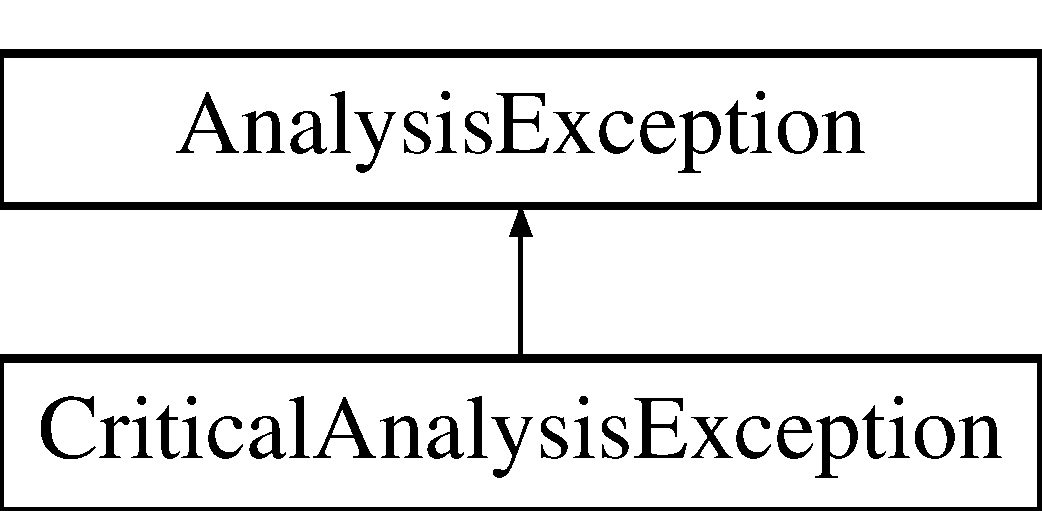
\includegraphics[height=2.000000cm]{classCriticalAnalysisException}
\end{center}
\end{figure}
\subsubsection*{Public Member Functions}
\begin{DoxyCompactItemize}
\item 
\hypertarget{classCriticalAnalysisException_a6d8c2626ca573a0cc7e70da8edb4c602}{
{\bfseries CriticalAnalysisException} (const std::string \&str)}
\label{classCriticalAnalysisException_a6d8c2626ca573a0cc7e70da8edb4c602}

\end{DoxyCompactItemize}


\subsubsection{Detailed Description}
Thrown on errors in the analysis where the program cannot recover. 

Definition at line 29 of file Exceptions.h.



The documentation for this class was generated from the following file:\begin{DoxyCompactItemize}
\item 
Exceptions.h\end{DoxyCompactItemize}

\hypertarget{structCut}{
\subsection{Cut Struct Reference}
\label{structCut}\index{Cut@{Cut}}
}


Describes range of values of a parameter to retain after cuts.  




{\ttfamily \#include $<$Config.h$>$}

\subsubsection*{Public Attributes}
\begin{DoxyCompactItemize}
\item 
\hypertarget{structCut_aa0560d0308b923448e508724147f69d8}{
double {\bfseries lower}}
\label{structCut_aa0560d0308b923448e508724147f69d8}

\item 
\hypertarget{structCut_a2ef70208b9fe13cf032fcc258514ed18}{
double {\bfseries upper}}
\label{structCut_a2ef70208b9fe13cf032fcc258514ed18}

\end{DoxyCompactItemize}


\subsubsection{Detailed Description}
Describes range of values of a parameter to retain after cuts. 

Definition at line 32 of file Config.h.



The documentation for this struct was generated from the following file:\begin{DoxyCompactItemize}
\item 
Config.h\end{DoxyCompactItemize}

\hypertarget{classCutFactory}{
\subsection{CutFactory Class Reference}
\label{classCutFactory}\index{CutFactory@{CutFactory}}
}


Responsible for locating files and creating the correct data reader object for the detected file type.  




{\ttfamily \#include $<$SuperCutter.h$>$}

\subsubsection*{Public Member Functions}
\begin{DoxyCompactItemize}
\item 
\hypertarget{classCutFactory_a521335d9a469768d33768786aecf33fb}{
\hyperlink{classSuperCutter}{SuperCutter} $\ast$ {\bfseries newCutter} (const \hyperlink{classRunInfo}{RunInfo} \&ri)}
\label{classCutFactory_a521335d9a469768d33768786aecf33fb}

\end{DoxyCompactItemize}
\subsubsection*{Static Public Member Functions}
\begin{DoxyCompactItemize}
\item 
\hypertarget{classCutFactory_a457083853ded569db341d1b8603e021c}{
static \hyperlink{classCutFactory}{CutFactory} $\ast$ \hyperlink{classCutFactory_a457083853ded569db341d1b8603e021c}{instance} ()}
\label{classCutFactory_a457083853ded569db341d1b8603e021c}

\end{DoxyCompactItemize}


\subsubsection{Detailed Description}
Responsible for locating files and creating the correct data reader object for the detected file type. 

Implemented as a Singleton. 

Definition at line 139 of file SuperCutter.h.



The documentation for this class was generated from the following files:\begin{DoxyCompactItemize}
\item 
SuperCutter.h\item 
SuperCutter.cpp\end{DoxyCompactItemize}

\hypertarget{structCutInfo}{
\subsection{CutInfo Struct Reference}
\label{structCutInfo}\index{CutInfo@{CutInfo}}
}


Describes which cuts should be applied to the data.  




{\ttfamily \#include $<$Config.h$>$}

\subsubsection*{Public Attributes}
\begin{DoxyCompactItemize}
\item 
\hypertarget{structCutInfo_a106a0ff9158531ad231e8a35f0780115}{
double {\bfseries tracking\_\-ratio}}
\label{structCutInfo_a106a0ff9158531ad231e8a35f0780115}

\item 
\hypertarget{structCutInfo_a74caf842b770af7717058c023aaab6e6}{
double \hyperlink{structCutInfo_a74caf842b770af7717058c023aaab6e6}{elongation}}
\label{structCutInfo_a74caf842b770af7717058c023aaab6e6}

\item 
\hypertarget{structCutInfo_ac11dc7dcd25917e62a1cfb54e37849b9}{
\hyperlink{structCut}{Cut} {\bfseries alpha}}
\label{structCutInfo_ac11dc7dcd25917e62a1cfb54e37849b9}

\item 
\hypertarget{structCutInfo_a6e54150661e34dd9068b04b1d13cf99a}{
\hyperlink{structCut}{Cut} {\bfseries distance}}
\label{structCutInfo_a6e54150661e34dd9068b04b1d13cf99a}

\item 
\hypertarget{structCutInfo_a64686c58c49e0a090b77d6053e8af1b5}{
\hyperlink{structCut}{Cut} {\bfseries length}}
\label{structCutInfo_a64686c58c49e0a090b77d6053e8af1b5}

\item 
\hypertarget{structCutInfo_ac71db39310190ea1db633eac8f5670d3}{
\hyperlink{structCut}{Cut} {\bfseries width}}
\label{structCutInfo_ac71db39310190ea1db633eac8f5670d3}

\item 
\hypertarget{structCutInfo_ad7c74fbec9d41def251a53d8dd3de8bd}{
\hyperlink{structCut}{Cut} {\bfseries size}}
\label{structCutInfo_ad7c74fbec9d41def251a53d8dd3de8bd}

\item 
\hypertarget{structCutInfo_a180779ebcc52ebded805398925af554f}{
\hyperlink{structCut}{Cut} {\bfseries lensize}}
\label{structCutInfo_a180779ebcc52ebded805398925af554f}

\item 
\hypertarget{structCutInfo_aaf30156f42f305da4e5775264a240df1}{
\hyperlink{structCut}{Cut} {\bfseries max1}}
\label{structCutInfo_aaf30156f42f305da4e5775264a240df1}

\item 
\hypertarget{structCutInfo_a7c71aadcb6f78607f6f76aeb282bf376}{
\hyperlink{structCut}{Cut} {\bfseries max2}}
\label{structCutInfo_a7c71aadcb6f78607f6f76aeb282bf376}

\item 
\hypertarget{structCutInfo_a4fc64eada4b44c8a67ee1d98f01515e9}{
\hyperlink{structCut}{Cut} {\bfseries max3}}
\label{structCutInfo_a4fc64eada4b44c8a67ee1d98f01515e9}

\item 
\hypertarget{structCutInfo_ad1e0e308d90331c7287995a5e01986fd}{
\hyperlink{structCut}{Cut} {\bfseries frac3}}
\label{structCutInfo_ad1e0e308d90331c7287995a5e01986fd}

\item 
\hypertarget{structCutInfo_a91a8fda67d4c28bb614b36b9957038ce}{
\hyperlink{structCut}{Cut} {\bfseries asymmdist}}
\label{structCutInfo_a91a8fda67d4c28bb614b36b9957038ce}

\item 
\hypertarget{structCutInfo_ab09d79624c928f5d9609ec2a827697cd}{
double {\bfseries dlength}}
\label{structCutInfo_ab09d79624c928f5d9609ec2a827697cd}

\item 
\hypertarget{structCutInfo_a3ba00a049c96eb81c8dcbf9ef0e9a307}{
double {\bfseries dwidth}}
\label{structCutInfo_a3ba00a049c96eb81c8dcbf9ef0e9a307}

\item 
\hypertarget{structCutInfo_afaa94e4416616984034d8c72be2f9544}{
double \hyperlink{structCutInfo_afaa94e4416616984034d8c72be2f9544}{smoothing\_\-radius}}
\label{structCutInfo_afaa94e4416616984034d8c72be2f9544}

\item 
\hypertarget{structCutInfo_ab9e09c8781c256d2e8b67ef2c5952700}{
bool \hyperlink{structCutInfo_ab9e09c8781c256d2e8b67ef2c5952700}{radial\_\-analysis}}
\label{structCutInfo_ab9e09c8781c256d2e8b67ef2c5952700}

\item 
\hypertarget{structCutInfo_a567c078c8001f34be48af8e2766e7a8b}{
\hyperlink{structCoordinate__t}{Coordinate\_\-t} \hyperlink{structCutInfo_a567c078c8001f34be48af8e2766e7a8b}{radial\_\-offset}}
\label{structCutInfo_a567c078c8001f34be48af8e2766e7a8b}

\item 
\hypertarget{structCutInfo_a04bbf876987e358d0a1901dec333518f}{
bool \hyperlink{structCutInfo_a04bbf876987e358d0a1901dec333518f}{alignment}}
\label{structCutInfo_a04bbf876987e358d0a1901dec333518f}

\item 
\hypertarget{structCutInfo_a2d0e84511f4a54ea16f8beb13b26442d}{
\hyperlink{structCoordinate__t}{Coordinate\_\-t} \hyperlink{structCutInfo_a2d0e84511f4a54ea16f8beb13b26442d}{align\_\-offset}}
\label{structCutInfo_a2d0e84511f4a54ea16f8beb13b26442d}

\end{DoxyCompactItemize}
\subsubsection*{Friends}
\begin{DoxyCompactItemize}
\item 
\hypertarget{structCutInfo_a14e393f2eee5a528b1a82cf1a869d5aa}{
std::ostream \& {\bfseries operator$<$$<$} (std::ostream \&stream, const \hyperlink{structCutInfo}{CutInfo} \&c)}
\label{structCutInfo_a14e393f2eee5a528b1a82cf1a869d5aa}

\end{DoxyCompactItemize}


\subsubsection{Detailed Description}
Describes which cuts should be applied to the data. 

Fields with upper and lower values are arrays with 2 elements. 

Definition at line 45 of file Config.h.



The documentation for this struct was generated from the following file:\begin{DoxyCompactItemize}
\item 
Config.h\end{DoxyCompactItemize}

\hypertarget{structCutRecord}{
\subsection{CutRecord Struct Reference}
\label{structCutRecord}\index{CutRecord@{CutRecord}}
}


Output from \hyperlink{classCutter}{Cutter} for each run...  




{\ttfamily \#include $<$DataRecords.h$>$}

Inheritance diagram for CutRecord:\begin{figure}[H]
\begin{center}
\leavevmode
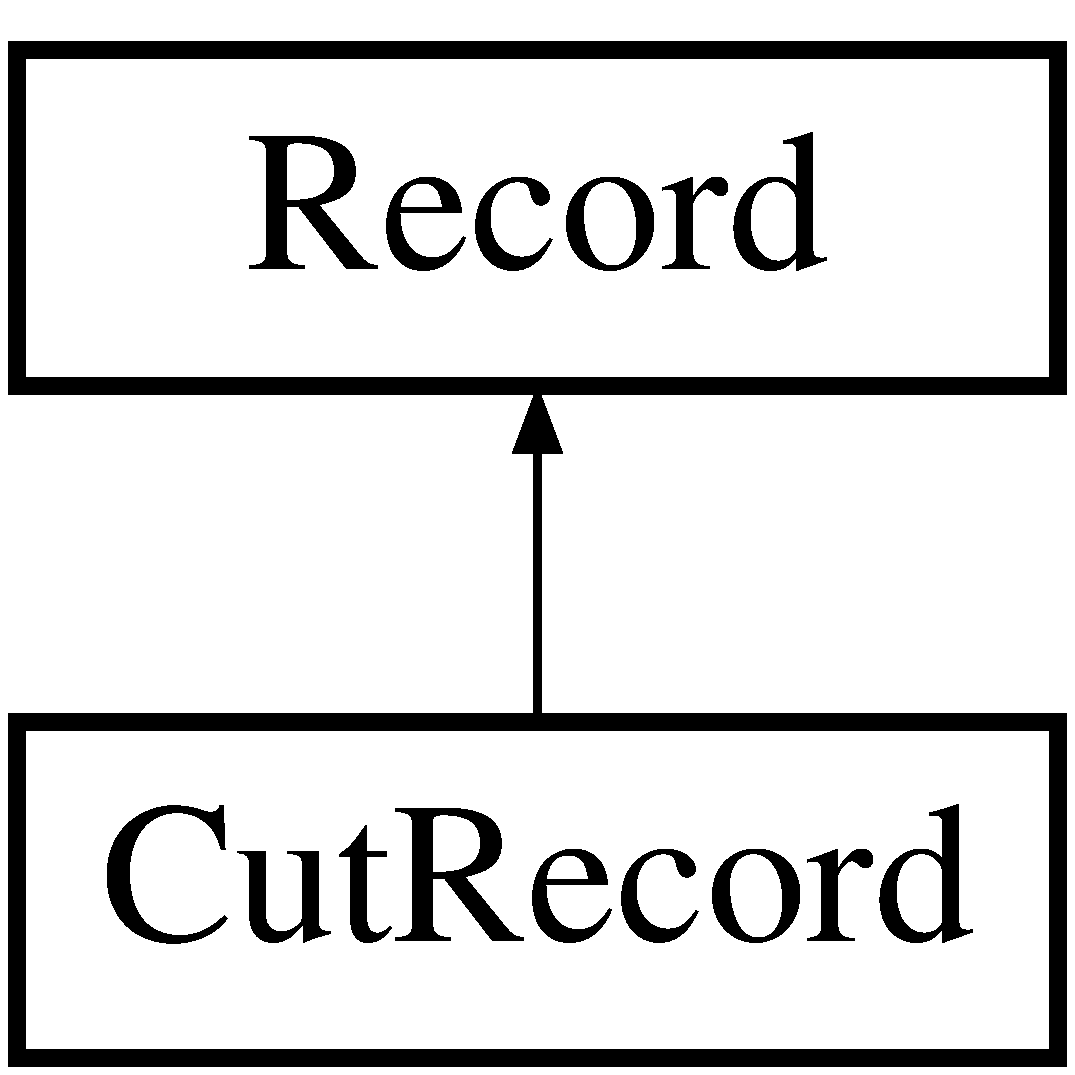
\includegraphics[height=2.000000cm]{structCutRecord}
\end{center}
\end{figure}
\subsubsection*{Public Member Functions}
\begin{DoxyCompactItemize}
\item 
\hypertarget{structCutRecord_a92a14da954641fc1d4803c6b1984b71f}{
void {\bfseries addValuesFrom} (\hyperlink{structCutRecord}{CutRecord} \&cr)}
\label{structCutRecord_a92a14da954641fc1d4803c6b1984b71f}

\end{DoxyCompactItemize}
\subsubsection*{Public Attributes}
\begin{DoxyCompactItemize}
\item 
\hypertarget{structCutRecord_adfcd254d32db32f1d1307083d852a2b7}{
std::string {\bfseries runid}}
\label{structCutRecord_adfcd254d32db32f1d1307083d852a2b7}

\item 
\hypertarget{structCutRecord_a82f38ab86e0998514ed9eca587655610}{
int {\bfseries total}}
\label{structCutRecord_a82f38ab86e0998514ed9eca587655610}

\item 
\hypertarget{structCutRecord_ae6574b47e0294354bba25bf8fcfdb39b}{
int {\bfseries valid}}
\label{structCutRecord_ae6574b47e0294354bba25bf8fcfdb39b}

\item 
\hypertarget{structCutRecord_ae59e52e0151453c25528ac04dc323b5e}{
int {\bfseries trigger}}
\label{structCutRecord_ae59e52e0151453c25528ac04dc323b5e}

\item 
\hypertarget{structCutRecord_a4f59a9828144aee6cdde202a1058852e}{
int {\bfseries shape}}
\label{structCutRecord_a4f59a9828144aee6cdde202a1058852e}

\item 
\hypertarget{structCutRecord_ae91f2917f8471a9e30c9657b33052349}{
int {\bfseries orientation}}
\label{structCutRecord_ae91f2917f8471a9e30c9657b33052349}

\item 
\hypertarget{structCutRecord_a48cce8675c3f2acd1743a92b16cd312a}{
int {\bfseries trackoff}}
\label{structCutRecord_a48cce8675c3f2acd1743a92b16cd312a}

\item 
\hypertarget{structCutRecord_af7ad09d587479c5de2b36dcb0ba21762}{
double {\bfseries duration}}
\label{structCutRecord_af7ad09d587479c5de2b36dcb0ba21762}

\item 
\hypertarget{structCutRecord_a6ab6f0a4063648aa67971658d5810405}{
double {\bfseries average\_\-elevation}}
\label{structCutRecord_a6ab6f0a4063648aa67971658d5810405}

\item 
\hypertarget{structCutRecord_a194cfd65fb7cb6e746867b0e81440b2c}{
\hyperlink{classImage2D}{Image2D} {\bfseries im2d}}
\label{structCutRecord_a194cfd65fb7cb6e746867b0e81440b2c}

\item 
\hypertarget{structCutRecord_acf725e77a2798fc393d554cadc93ae78}{
\hyperlink{classImage2D}{Image2D} {\bfseries skybright}}
\label{structCutRecord_acf725e77a2798fc393d554cadc93ae78}

\item 
\hypertarget{structCutRecord_a1f48a29681a74f0efd706e18129f2317}{
\hyperlink{classImage2D}{Image2D} {\bfseries tubeoff}}
\label{structCutRecord_a1f48a29681a74f0efd706e18129f2317}

\item 
\hypertarget{structCutRecord_a560f83767534600d512b93522ea3ad25}{
std::vector$<$ \hyperlink{structCoordinate__t}{Coordinate\_\-t} $>$ {\bfseries poolist}}
\label{structCutRecord_a560f83767534600d512b93522ea3ad25}

\end{DoxyCompactItemize}


\subsubsection{Detailed Description}
Output from \hyperlink{classCutter}{Cutter} for each run... 

Definition at line 90 of file DataRecords.h.



The documentation for this struct was generated from the following file:\begin{DoxyCompactItemize}
\item 
DataRecords.h\end{DoxyCompactItemize}

\hypertarget{classCutRunInfo}{
\subsection{CutRunInfo Class Reference}
\label{classCutRunInfo}\index{CutRunInfo@{CutRunInfo}}
}


\hyperlink{classParamRunInfo}{ParamRunInfo} + cut information.  




{\ttfamily \#include $<$DataRecords.h$>$}

Inheritance diagram for CutRunInfo:\begin{figure}[H]
\begin{center}
\leavevmode
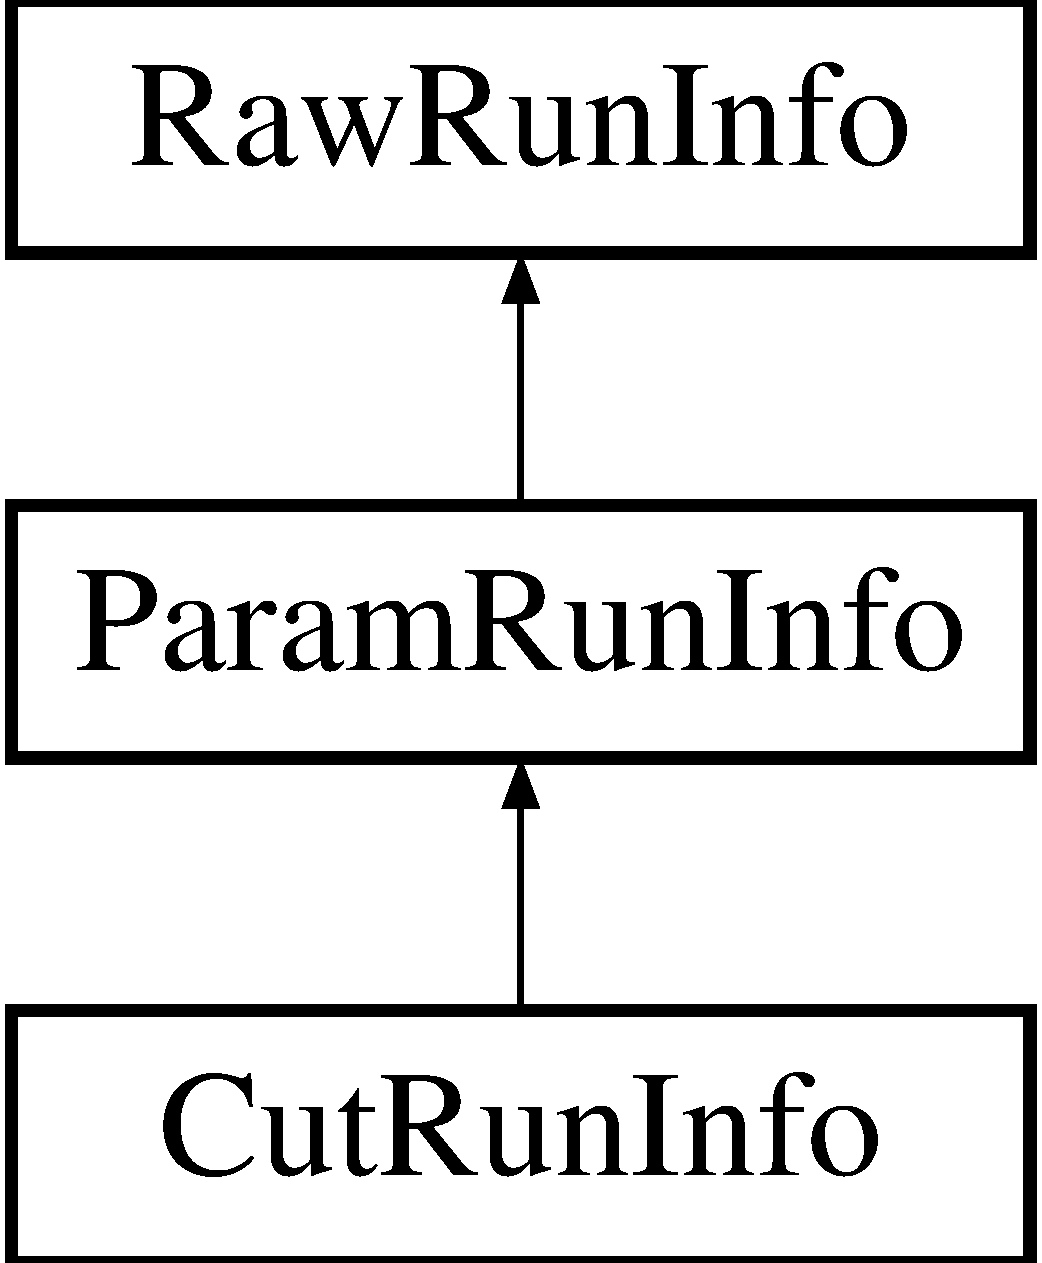
\includegraphics[height=3.000000cm]{classCutRunInfo}
\end{center}
\end{figure}
\subsubsection*{Public Attributes}
\begin{DoxyCompactItemize}
\item 
\hypertarget{classCutRunInfo_a711281ce18c77ebd12a7910ab1841b7c}{
int {\bfseries total}}
\label{classCutRunInfo_a711281ce18c77ebd12a7910ab1841b7c}

\item 
\hypertarget{classCutRunInfo_acfadf61bb4cf234c443d87708774fe81}{
int {\bfseries valid}}
\label{classCutRunInfo_acfadf61bb4cf234c443d87708774fe81}

\item 
\hypertarget{classCutRunInfo_aa9d2bf43e7f23a1650de5c7ffb20e79b}{
int {\bfseries trigger}}
\label{classCutRunInfo_aa9d2bf43e7f23a1650de5c7ffb20e79b}

\item 
\hypertarget{classCutRunInfo_a49356d438070918c81c80698850161bf}{
int {\bfseries shape}}
\label{classCutRunInfo_a49356d438070918c81c80698850161bf}

\item 
\hypertarget{classCutRunInfo_a349308b08b4041bdfaea2a06d82ab86e}{
int {\bfseries orientation}}
\label{classCutRunInfo_a349308b08b4041bdfaea2a06d82ab86e}

\item 
\hypertarget{classCutRunInfo_a69c3b28457dcb2ce78a76820f9137fbd}{
int {\bfseries trackoff}}
\label{classCutRunInfo_a69c3b28457dcb2ce78a76820f9137fbd}

\item 
\hypertarget{classCutRunInfo_a86dc52ebd1a40a23b855fce85a0329b5}{
double {\bfseries duration}}
\label{classCutRunInfo_a86dc52ebd1a40a23b855fce85a0329b5}

\end{DoxyCompactItemize}


\subsubsection{Detailed Description}
\hyperlink{classParamRunInfo}{ParamRunInfo} + cut information. 

Definition at line 188 of file DataRecords.h.



The documentation for this class was generated from the following file:\begin{DoxyCompactItemize}
\item 
DataRecords.h\end{DoxyCompactItemize}

\hypertarget{classCutter}{
\subsection{Cutter Class Reference}
\label{classCutter}\index{Cutter@{Cutter}}
}


\hyperlink{namespaceCuts}{Cuts} parameterized data, calculates statistics, and generates final histograms.  




{\ttfamily \#include $<$Cutter.h$>$}

\subsubsection*{Public Types}
\begin{DoxyCompactItemize}
\item 
enum {\bfseries types} \{ {\bfseries ON}, 
{\bfseries OFF}, 
{\bfseries TRACK}
 \}
\end{DoxyCompactItemize}
\subsubsection*{Public Member Functions}
\begin{DoxyCompactItemize}
\item 
\hypertarget{classCutter_af2b736c98364bced8a589af6c2a23876}{
void {\bfseries enableOutput} (bool val=1)}
\label{classCutter_af2b736c98364bced8a589af6c2a23876}

\item 
\hypertarget{classCutter_ae91898ee742899ce553a0950a4649d6e}{
void {\bfseries enableScaledParameterOutput} (bool val=1)}
\label{classCutter_ae91898ee742899ce553a0950a4649d6e}

\item 
\hypertarget{classCutter_af8f718594f826e6da8c3cb80b8e233cc}{
void {\bfseries enableFastImageProcessing} (bool val=1)}
\label{classCutter_af8f718594f826e6da8c3cb80b8e233cc}

\item 
\hypertarget{classCutter_a5074fd0776b5c706d6e4ec932fefd74f}{
void {\bfseries enable2D} (bool val=1)}
\label{classCutter_a5074fd0776b5c706d6e4ec932fefd74f}

\item 
\hypertarget{classCutter_a6f7d668a1314d47cf04c9f0ff512f00b}{
void {\bfseries enablePointingCheck} (bool val=true)}
\label{classCutter_a6f7d668a1314d47cf04c9f0ff512f00b}

\item 
\hypertarget{classCutter_a8a6b24a2596e6cb48e5a64583c9000cb}{
void {\bfseries enableDisplay} (bool val=true)}
\label{classCutter_a8a6b24a2596e6cb48e5a64583c9000cb}

\item 
void \hyperlink{classCutter_a2c7e98e45d19df45fb23652a4a40cf38}{process} (\hyperlink{classRunInfo}{RunInfo} \&ri)
\item 
\hypertarget{classCutter_afe5b50816216132d772fba55c84d4585}{
\hyperlink{structRunStatistics}{RunStatistics} {\bfseries getTrackingStatistics} (\hyperlink{structCutRecord}{CutRecord} \&run, double ratio)}
\label{classCutter_afe5b50816216132d772fba55c84d4585}

\item 
\hypertarget{classCutter_af137a9fa058a3e8b2428dcbc8d4edf4f}{
\hyperlink{structRunStatistics}{RunStatistics} {\bfseries getPairStatistics} (\hyperlink{structCutRecord}{CutRecord} \&onrun, \hyperlink{structCutRecord}{CutRecord} \&offrun)}
\label{classCutter_af137a9fa058a3e8b2428dcbc8d4edf4f}

\item 
\hypertarget{classCutter_ab5ebc8264e083c5aa66a558f033f78d0}{
\hyperlink{structRunStatistics}{RunStatistics} {\bfseries getTotalPairStatistics} ()}
\label{classCutter_ab5ebc8264e083c5aa66a558f033f78d0}

\item 
\hypertarget{classCutter_a3e456388ddb758748a3b69c8683c0b5a}{
void \hyperlink{classCutter_a3e456388ddb758748a3b69c8683c0b5a}{outputStatistics} ()}
\label{classCutter_a3e456388ddb758748a3b69c8683c0b5a}

\item 
double \hyperlink{classCutter_a2eb708059e0d94349cfa92bdc7551c0b}{energyEstimator} (double size, double dist)
\item 
\hypertarget{classCutter_ad46d67859c5fc57e7efc2936fabca360}{
\hyperlink{structCutRecord}{CutRecord} {\bfseries getTotal} (std::vector$<$ \hyperlink{structCutRecord}{CutRecord} $>$ \&)}
\label{classCutter_ad46d67859c5fc57e7efc2936fabca360}

\item 
double \hyperlink{classCutter_a502eab82b5602adadaa76c7cdb9326d6}{maxLikelihoodSignif} (double n\_\-on, double n\_\-off, double alpha)
\item 
\hyperlink{structCutRecord}{CutRecord} \hyperlink{classCutter_a5c8d71e05e508ec60db78436b4ba416d}{cut} (\hyperlink{classRunInfo}{RunInfo} \&, const std::string \&, char)
\item 
void \hyperlink{classCutter_ac4a14824d14bc9a15e61d6a09a7a4b62}{generateImage} (\hyperlink{structCutRecord}{CutRecord} \&on, \hyperlink{structCutRecord}{CutRecord} \&off, std::string dir, std::string title, bool finalimage=false)
\item 
\hypertarget{classCutter_a6caf41bc19118ac547af26c61282e6db}{
void {\bfseries radiallyBinPoints} (std::vector$<$ \hyperlink{structCoordinate__t}{Coordinate\_\-t} $>$ \&poolist, \hyperlink{classImage2D}{Image2D} \&destimage, double radius)}
\label{classCutter_a6caf41bc19118ac547af26c61282e6db}

\item 
\hypertarget{classCutter_ae6ed9e84dca55866f7ceeea402c5a9b9}{
void {\bfseries setOutputDir} (std::string dirname)}
\label{classCutter_ae6ed9e84dca55866f7ceeea402c5a9b9}

\item 
\hypertarget{classCutter_a4583bb71d7ae87f6d2dd1ca0fc5e1a45}{
void {\bfseries printCutRecordFields} (std::ostream \&stream)}
\label{classCutter_a4583bb71d7ae87f6d2dd1ca0fc5e1a45}

\item 
\hypertarget{classCutter_a3149fbadf8d441d6506a49bc1a3f37fb}{
void \hyperlink{classCutter_a3149fbadf8d441d6506a49bc1a3f37fb}{checkPointing} ()}
\label{classCutter_a3149fbadf8d441d6506a49bc1a3f37fb}

\item 
\hypertarget{classCutter_a749513671e6f22e31587fd472844c3df}{
void \hyperlink{classCutter_a749513671e6f22e31587fd472844c3df}{checkDiagnostics} ()}
\label{classCutter_a749513671e6f22e31587fd472844c3df}

\item 
double \hyperlink{classCutter_a3c92b110a34487b1a20740eb7d395b20}{getElongationFactor} (double zenith)
\item 
\hypertarget{classCutter_adf08fb8b5af263109ca7b9e24f327bc3}{
void {\bfseries setTelescopeID} (int num)}
\label{classCutter_adf08fb8b5af263109ca7b9e24f327bc3}

\item 
\hypertarget{classCutter_a202368215c24637b30e9b38107fe3036}{
void {\bfseries clear} ()}
\label{classCutter_a202368215c24637b30e9b38107fe3036}

\end{DoxyCompactItemize}


\subsubsection{Detailed Description}
\hyperlink{namespaceCuts}{Cuts} parameterized data, calculates statistics, and generates final histograms. 

\begin{Desc}
\item[\hyperlink{todo__todo000006}{Todo}]: this is a badly designed class. \hyperlink{classCutter}{Cutter} should be a small object which applies a specific set of cuts (subclasses for other cutting methods). All the analysis should be done elsewhere.\end{Desc}


\begin{Desc}
\item[\hyperlink{todo__todo000007}{Todo}]: For multi-\/telescope analysis, make a telescope\_\-id argument or field and only process events from the specified telescope. \end{Desc}


Definition at line 39 of file Cutter.h.



\subsubsection{Member Function Documentation}
\hypertarget{classCutter_a5c8d71e05e508ec60db78436b4ba416d}{
\index{Cutter@{Cutter}!cut@{cut}}
\index{cut@{cut}!Cutter@{Cutter}}
\paragraph[{cut}]{\setlength{\rightskip}{0pt plus 5cm}{\bf CutRecord} Cutter::cut (
\begin{DoxyParamCaption}
\item[{{\bf RunInfo} \&}]{, }
\item[{const std::string \&}]{, }
\item[{char}]{}
\end{DoxyParamCaption}
)}}
\label{classCutter_a5c8d71e05e508ec60db78436b4ba416d}


Read the parameterized data for the specified run id and count the number of events that pass the various cuts. 

Also generates histograms of rate, size, energy, etc. This function is called by \hyperlink{classCutter_a2c7e98e45d19df45fb23652a4a40cf38}{Cutter::process} for each run in the configuration file, so there is usually no need to call it directly.

\begin{DoxyReturn}{Returns}
a \hyperlink{structCutRecord}{CutRecord} containing all the totals for the specified run.
\end{DoxyReturn}
\begin{Desc}
\item[\hyperlink{todo__todo000004}{Todo}]: Implement 2-\/D analysis for tracking runs (currently, only ON/OFF pairs are used.\end{Desc}


\begin{Desc}
\item[\hyperlink{todo__todo000005}{Todo}]: separate total alpha plot for tracking runs.\end{Desc}


Definition at line 1162 of file Cutter.cpp.



References Image2D::addHist(), CutInfo::align\_\-offset, CutInfo::alignment, HillasParameterization::alpha, SuperCutter::applyCorrections(), HeaderRecord::average\_\-elevation, HillasParameterization::centroid, Image2D::clear(), RunInfo::cuts, RunInfo::cuttype, HeaderRecord::dec, HillasParameterization::distance, HeaderRecord::endtime, HillasParameterization::energy\_\-estimate, RunInfo::energyestimator, StarCatalog::findNearbyStars(), ParamDataReader::getHeaderRecord(), ImageParameterization::gpstime, Histogram::increment(), CutFactory::instance(), EnergyEstimatorFactory::instance(), HeaderRecord::nadc, HeaderRecord::num\_\-telescopes, SuperCutter::pass(), PlotMaker::plotAxes(), HillasParameterization::point\_\-of\_\-origin\_\-a, HillasParameterization::point\_\-of\_\-origin\_\-b, StarCatalog::precessToDate(), HeaderRecord::ra, CutInfo::radial\_\-analysis, CutInfo::radial\_\-offset, Image2D::save(), Image2D::setCoordinateBox(), HillasParameterization::size, CutInfo::smoothing\_\-radius, HeaderRecord::sourcename, HeaderRecord::starttime, ImageParameterization::telescope\_\-id, RunInfo::utbase, RunInfo::utdate, Coordinate\_\-t::x, Coordinate\_\-t::y, and HillasParameterization::zenith.



Referenced by process().

\hypertarget{classCutter_a2eb708059e0d94349cfa92bdc7551c0b}{
\index{Cutter@{Cutter}!energyEstimator@{energyEstimator}}
\index{energyEstimator@{energyEstimator}!Cutter@{Cutter}}
\paragraph[{energyEstimator}]{\setlength{\rightskip}{0pt plus 5cm}double Cutter::energyEstimator (
\begin{DoxyParamCaption}
\item[{double}]{size, }
\item[{double}]{dist}
\end{DoxyParamCaption}
)}}
\label{classCutter_a2eb708059e0d94349cfa92bdc7551c0b}


Return the energy estimate for the given size and distance values. 

\begin{DoxyReturn}{Returns}
x = log(Energy) 
\end{DoxyReturn}


Definition at line 1664 of file Cutter.cpp.

\hypertarget{classCutter_ac4a14824d14bc9a15e61d6a09a7a4b62}{
\index{Cutter@{Cutter}!generateImage@{generateImage}}
\index{generateImage@{generateImage}!Cutter@{Cutter}}
\paragraph[{generateImage}]{\setlength{\rightskip}{0pt plus 5cm}void Cutter::generateImage (
\begin{DoxyParamCaption}
\item[{{\bf CutRecord} \&}]{on, }
\item[{{\bf CutRecord} \&}]{off, }
\item[{std::string}]{dir, }
\item[{std::string}]{title, }
\item[{bool}]{finalimage = {\ttfamily false}}
\end{DoxyParamCaption}
)}}
\label{classCutter_ac4a14824d14bc9a15e61d6a09a7a4b62}


Save a datafile (image2d-\/total.dat) containing the 2D excess and significance values for all of the data that has been currently cut. 

The format of the output file is 6 columns per line:
\begin{DoxyItemize}
\item column 1: x camera coordinate bin (in degrees)
\item column 2: y camera coordinate bin (in degrees)
\item column 3: excess counts
\item column 4: significance
\item column 5: Right Ascension of bin
\item column 6: Declination of bin 
\end{DoxyItemize}

Definition at line 832 of file Cutter.cpp.



References Image2D::addHistRadially(), Image2D::addImage(), Image2D::applyRadialSmoothing(), Image2D::expand(), maxLikelihoodSignif(), Image2D::save(), and Image2D::setCoordinateBox().



Referenced by outputStatistics(), and process().

\hypertarget{classCutter_a3c92b110a34487b1a20740eb7d395b20}{
\index{Cutter@{Cutter}!getElongationFactor@{getElongationFactor}}
\index{getElongationFactor@{getElongationFactor}!Cutter@{Cutter}}
\paragraph[{getElongationFactor}]{\setlength{\rightskip}{0pt plus 5cm}double Cutter::getElongationFactor (
\begin{DoxyParamCaption}
\item[{double}]{zen}
\end{DoxyParamCaption}
)}}
\label{classCutter_a3c92b110a34487b1a20740eb7d395b20}
\begin{DoxyReturn}{Returns}
zenith angle dependent elongation factor for the camera 
\end{DoxyReturn}


Definition at line 1687 of file Cutter.cpp.

\hypertarget{classCutter_a502eab82b5602adadaa76c7cdb9326d6}{
\index{Cutter@{Cutter}!maxLikelihoodSignif@{maxLikelihoodSignif}}
\index{maxLikelihoodSignif@{maxLikelihoodSignif}!Cutter@{Cutter}}
\paragraph[{maxLikelihoodSignif}]{\setlength{\rightskip}{0pt plus 5cm}double Cutter::maxLikelihoodSignif (
\begin{DoxyParamCaption}
\item[{double}]{n\_\-on, }
\item[{double}]{n\_\-off, }
\item[{double}]{alpha}
\end{DoxyParamCaption}
)}}
\label{classCutter_a502eab82b5602adadaa76c7cdb9326d6}


Returns the maximum likelihood significance (see Li and Ma, 1983) 


\begin{DoxyParams}{Parameters}
{\em n\_\-on} & number of on-\/source counts \\
\hline
{\em n\_\-off} & number of off-\/source counts \\
\hline
{\em alpha} & 1/(tracking ratio) for tracking runs, or on/off duration for on/off pairs.\\
\hline
\end{DoxyParams}
NOTE alpha is defined as 1/(tracking ratio) where the tracking ratio is the ratio of (number of off-\/source bins)/(on-\/source bins) So, e.g., for an \char`\"{}alpha\char`\"{} cut of alpha$<$15 for on-\/source and 20 $<$ alpha $<$ 65 for off-\/source, the tracking ratio = 3.0 and alpha = 0.333. Defining alpha in this way, excess = n\_\-on -\/ alpha $\ast$ n\_\-off. 

Definition at line 158 of file Cutter.cpp.



Referenced by generateImage().

\hypertarget{classCutter_a2c7e98e45d19df45fb23652a4a40cf38}{
\index{Cutter@{Cutter}!process@{process}}
\index{process@{process}!Cutter@{Cutter}}
\paragraph[{process}]{\setlength{\rightskip}{0pt plus 5cm}void Cutter::process (
\begin{DoxyParamCaption}
\item[{{\bf RunInfo} \&}]{ri}
\end{DoxyParamCaption}
)}}
\label{classCutter_a2c7e98e45d19df45fb23652a4a40cf38}


\hyperlink{structCut}{Cut} the data in the specified run, and build up statistics for all runs. 

Each run's cut information is stored in the onruns/offruns/trackruns vectors. 

Definition at line 1081 of file Cutter.cpp.



References cut(), RunInfo::cuts, generateImage(), RunInfo::offid, RunInfo::onid, Logger::printf(), CutInfo::radial\_\-analysis, CutInfo::smoothing\_\-radius, and RunInfo::type.



The documentation for this class was generated from the following files:\begin{DoxyCompactItemize}
\item 
Cutter.h\item 
Cutter.cpp\end{DoxyCompactItemize}

\hypertarget{structData}{
\subsection{Data Struct Reference}
\label{structData}\index{Data@{Data}}
}


We store the data in an Array, We only want to know the number of excess counts, and the variance of this number.  




{\ttfamily \#include $<$Fitter.h$>$}

\subsubsection*{Public Attributes}
\begin{DoxyCompactItemize}
\item 
\hypertarget{structData_a4785d0e7da0dfb26ec3284d6b6a1d680}{
double {\bfseries onOff}}
\label{structData_a4785d0e7da0dfb26ec3284d6b6a1d680}

\item 
\hypertarget{structData_af46d83f495c7ae27a04787e2ae0c33f8}{
double {\bfseries onOffVariance}}
\label{structData_af46d83f495c7ae27a04787e2ae0c33f8}

\end{DoxyCompactItemize}


\subsubsection{Detailed Description}
We store the data in an Array, We only want to know the number of excess counts, and the variance of this number. 

Definition at line 60 of file Fitter.h.



The documentation for this struct was generated from the following files:\begin{DoxyCompactItemize}
\item 
Fitter.h\item 
FitterNew.h\end{DoxyCompactItemize}

\hypertarget{classDataReader}{
\subsection{DataReader Class Reference}
\label{classDataReader}\index{DataReader@{DataReader}}
}


Base class for all data readers (raw, parameterized, cut)  




{\ttfamily \#include $<$DataReader.h$>$}

Inheritance diagram for DataReader:\begin{figure}[H]
\begin{center}
\leavevmode
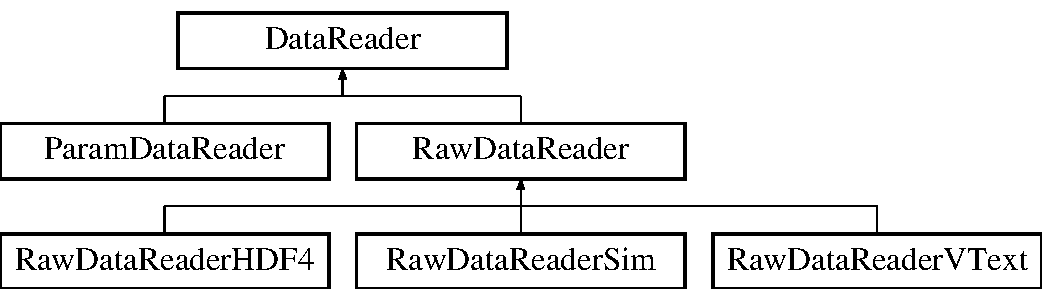
\includegraphics[height=3.000000cm]{classDataReader}
\end{center}
\end{figure}
\subsubsection*{Public Member Functions}
\begin{DoxyCompactItemize}
\item 
\hypertarget{classDataReader_aa905accd5935bffd48aba689f4f45c4c}{
{\bfseries DataReader} (const std::string \&filename)}
\label{classDataReader_aa905accd5935bffd48aba689f4f45c4c}

\item 
\hypertarget{classDataReader_a3390579e206a8b22b43f1d60ac86a423}{
std::string {\bfseries getFilename} ()}
\label{classDataReader_a3390579e206a8b22b43f1d60ac86a423}

\item 
\hypertarget{classDataReader_acc6161e84da4a6ff14eea42933590687}{
virtual bool {\bfseries isDone} ()=0}
\label{classDataReader_acc6161e84da4a6ff14eea42933590687}

\item 
\hypertarget{classDataReader_a5395e794e7e38edfb8d9492fdbed9293}{
virtual int {\bfseries size} ()=0}
\label{classDataReader_a5395e794e7e38edfb8d9492fdbed9293}

\item 
\hypertarget{classDataReader_a227c561f64239b508293e15d2dc78335}{
virtual std::string {\bfseries getTypeString} ()=0}
\label{classDataReader_a227c561f64239b508293e15d2dc78335}

\end{DoxyCompactItemize}


\subsubsection{Detailed Description}
Base class for all data readers (raw, parameterized, cut) 

Definition at line 21 of file DataReader.h.



The documentation for this class was generated from the following file:\begin{DoxyCompactItemize}
\item 
DataReader.h\end{DoxyCompactItemize}

\hypertarget{classDataWriter}{
\subsection{DataWriter Class Reference}
\label{classDataWriter}\index{DataWriter@{DataWriter}}
}


Base class for all data writers (parameterized data and cut data).  




{\ttfamily \#include $<$DataWriter.h$>$}

Inheritance diagram for DataWriter:\begin{figure}[H]
\begin{center}
\leavevmode
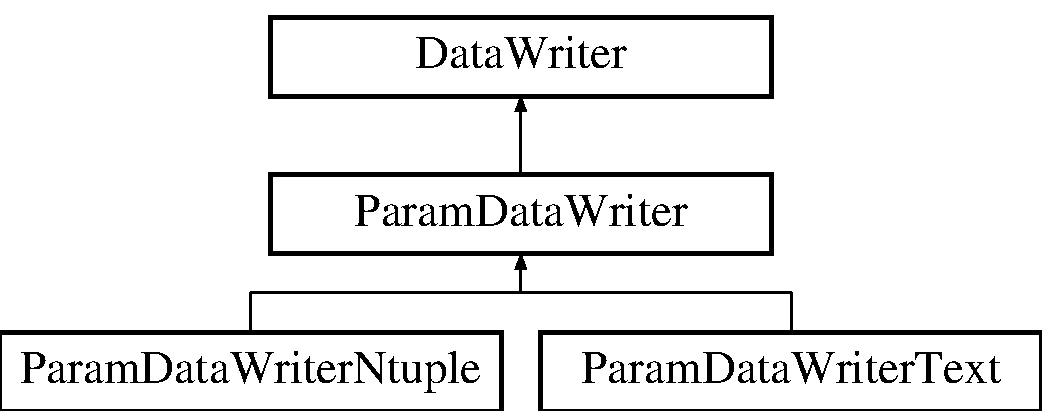
\includegraphics[height=3.000000cm]{classDataWriter}
\end{center}
\end{figure}
\subsubsection*{Public Member Functions}
\begin{DoxyCompactItemize}
\item 
\hypertarget{classDataWriter_aeeecf23712a2968038cdf7d309de3b50}{
{\bfseries DataWriter} (const std::string \&filename, bool=false)}
\label{classDataWriter_aeeecf23712a2968038cdf7d309de3b50}

\item 
\hypertarget{classDataWriter_a88be2fd630eb6bf633701d0b8c08306a}{
virtual std::string {\bfseries getTypeString} ()=0}
\label{classDataWriter_a88be2fd630eb6bf633701d0b8c08306a}

\item 
\hypertarget{classDataWriter_a1b3278ba4c5dd0922cdaf1bd7b866782}{
std::string {\bfseries getFilename} ()}
\label{classDataWriter_a1b3278ba4c5dd0922cdaf1bd7b866782}

\end{DoxyCompactItemize}


\subsubsection{Detailed Description}
Base class for all data writers (parameterized data and cut data). 

Specifies a standard interface. 

Definition at line 19 of file DataWriter.h.



The documentation for this class was generated from the following file:\begin{DoxyCompactItemize}
\item 
DataWriter.h\end{DoxyCompactItemize}

\hypertarget{classDefaultImageCleaner}{
\subsection{DefaultImageCleaner Class Reference}
\label{classDefaultImageCleaner}\index{DefaultImageCleaner@{DefaultImageCleaner}}
}


The default cleaner uses a simple 2 threshold process.  




{\ttfamily \#include $<$ImageCleaner.h$>$}

Inheritance diagram for DefaultImageCleaner:\begin{figure}[H]
\begin{center}
\leavevmode
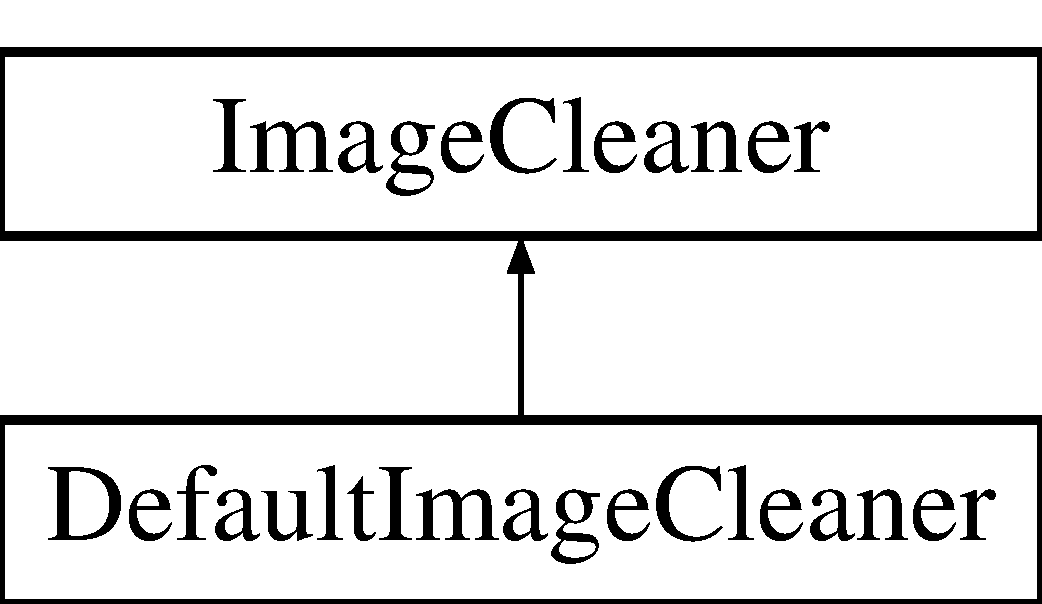
\includegraphics[height=2.000000cm]{classDefaultImageCleaner}
\end{center}
\end{figure}
\subsubsection*{Public Member Functions}
\begin{DoxyCompactItemize}
\item 
\hyperlink{classDefaultImageCleaner_af029b40ac6974bf0b3196c67bc5b34a0}{DefaultImageCleaner} (\hyperlink{classCamera}{Camera} \&camera, vector$<$ \hyperlink{structPedestal}{Pedestal} $>$ \&peds, double picture, double boundary)
\item 
\hypertarget{classDefaultImageCleaner_ae8b9d57c8aff0ffe07be81ee04b92255}{
std::vector$<$ int $>$ \& {\bfseries getCleanPixels} (const Array\_\-t \&image)}
\label{classDefaultImageCleaner_ae8b9d57c8aff0ffe07be81ee04b92255}

\end{DoxyCompactItemize}


\subsubsection{Detailed Description}
The default cleaner uses a simple 2 threshold process. 

Definition at line 33 of file ImageCleaner.h.



\subsubsection{Constructor \& Destructor Documentation}
\hypertarget{classDefaultImageCleaner_af029b40ac6974bf0b3196c67bc5b34a0}{
\index{DefaultImageCleaner@{DefaultImageCleaner}!DefaultImageCleaner@{DefaultImageCleaner}}
\index{DefaultImageCleaner@{DefaultImageCleaner}!DefaultImageCleaner@{DefaultImageCleaner}}
\paragraph[{DefaultImageCleaner}]{\setlength{\rightskip}{0pt plus 5cm}DefaultImageCleaner::DefaultImageCleaner (
\begin{DoxyParamCaption}
\item[{{\bf Camera} \&}]{camera, }
\item[{vector$<$ {\bf Pedestal} $>$ \&}]{peds, }
\item[{double}]{picture, }
\item[{double}]{boundary}
\end{DoxyParamCaption}
)}}
\label{classDefaultImageCleaner_af029b40ac6974bf0b3196c67bc5b34a0}


The default image cleaner uses picture and boundary theshold values (expressed in standard deviations from the pedestal) to determine the accepted pixels. 

All tubes above the picture threshold are accepted. Tubes above the boundary threshold with at least one neighboring \char`\"{}picture\char`\"{} tube are also accepted.


\begin{DoxyParams}{Parameters}
{\em camera} & reference to the camera object to use for pixel positions and neighborlist. \\
\hline
{\em peds} & reference to the \hyperlink{structPedestal}{Pedestal} array for the current run. \\
\hline
{\em picture} & the picture threshold in std deviations. \\
\hline
{\em boundary} & the boundary threhold in std deviations. \\
\hline
\end{DoxyParams}


Definition at line 25 of file ImageCleaner.cpp.



The documentation for this class was generated from the following files:\begin{DoxyCompactItemize}
\item 
ImageCleaner.h\item 
ImageCleaner.cpp\end{DoxyCompactItemize}

\hypertarget{structEnergyEstimator}{
\subsection{EnergyEstimator Struct Reference}
\label{structEnergyEstimator}\index{EnergyEstimator@{EnergyEstimator}}
}
Inheritance diagram for EnergyEstimator:\begin{figure}[H]
\begin{center}
\leavevmode
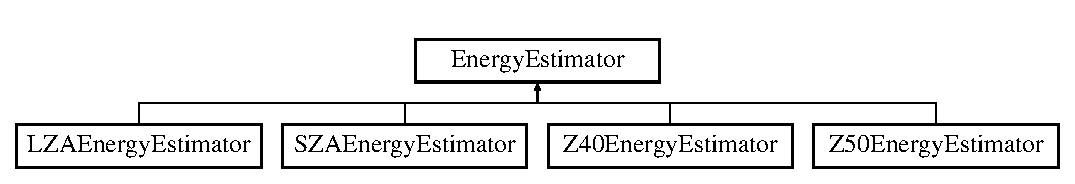
\includegraphics[height=2.000000cm]{structEnergyEstimator}
\end{center}
\end{figure}
\subsubsection*{Public Member Functions}
\begin{DoxyCompactItemize}
\item 
\hypertarget{structEnergyEstimator_a72b73d1cdaa39c43e6ec4a80a9e74aaa}{
virtual double {\bfseries getEstimate} (const double size, const double distance, const double zenith)=0}
\label{structEnergyEstimator_a72b73d1cdaa39c43e6ec4a80a9e74aaa}

\end{DoxyCompactItemize}


\subsubsection{Detailed Description}


Definition at line 36 of file EnergySpectrum.h.



The documentation for this struct was generated from the following file:\begin{DoxyCompactItemize}
\item 
EnergySpectrum.h\end{DoxyCompactItemize}

\hypertarget{classEnergyEstimatorFactory}{
\subsection{EnergyEstimatorFactory Class Reference}
\label{classEnergyEstimatorFactory}\index{EnergyEstimatorFactory@{EnergyEstimatorFactory}}
}
\subsubsection*{Public Member Functions}
\begin{DoxyCompactItemize}
\item 
\hypertarget{classEnergyEstimatorFactory_aec2a2f82f0fe51b26557e046de5bec82}{
\hyperlink{structEnergyEstimator}{EnergyEstimator} $\ast$ {\bfseries getEstimator} (std::string type)}
\label{classEnergyEstimatorFactory_aec2a2f82f0fe51b26557e046de5bec82}

\end{DoxyCompactItemize}
\subsubsection*{Static Public Member Functions}
\begin{DoxyCompactItemize}
\item 
\hypertarget{classEnergyEstimatorFactory_af654e8785f7012147fd5467451053890}{
static \hyperlink{classEnergyEstimatorFactory}{EnergyEstimatorFactory} $\ast$ \hyperlink{classEnergyEstimatorFactory_af654e8785f7012147fd5467451053890}{instance} ()}
\label{classEnergyEstimatorFactory_af654e8785f7012147fd5467451053890}

\end{DoxyCompactItemize}


\subsubsection{Detailed Description}


Definition at line 65 of file EnergySpectrum.h.



The documentation for this class was generated from the following files:\begin{DoxyCompactItemize}
\item 
EnergySpectrum.h\item 
EnergySpectrum.cpp\end{DoxyCompactItemize}

\hypertarget{classEnergySpectrum}{
\subsection{EnergySpectrum Class Reference}
\label{classEnergySpectrum}\index{EnergySpectrum@{EnergySpectrum}}
}


Energy Spectrum 1-\/D histogram class.  




{\ttfamily \#include $<$EnergySpectrum.h$>$}

Inheritance diagram for EnergySpectrum:\begin{figure}[H]
\begin{center}
\leavevmode
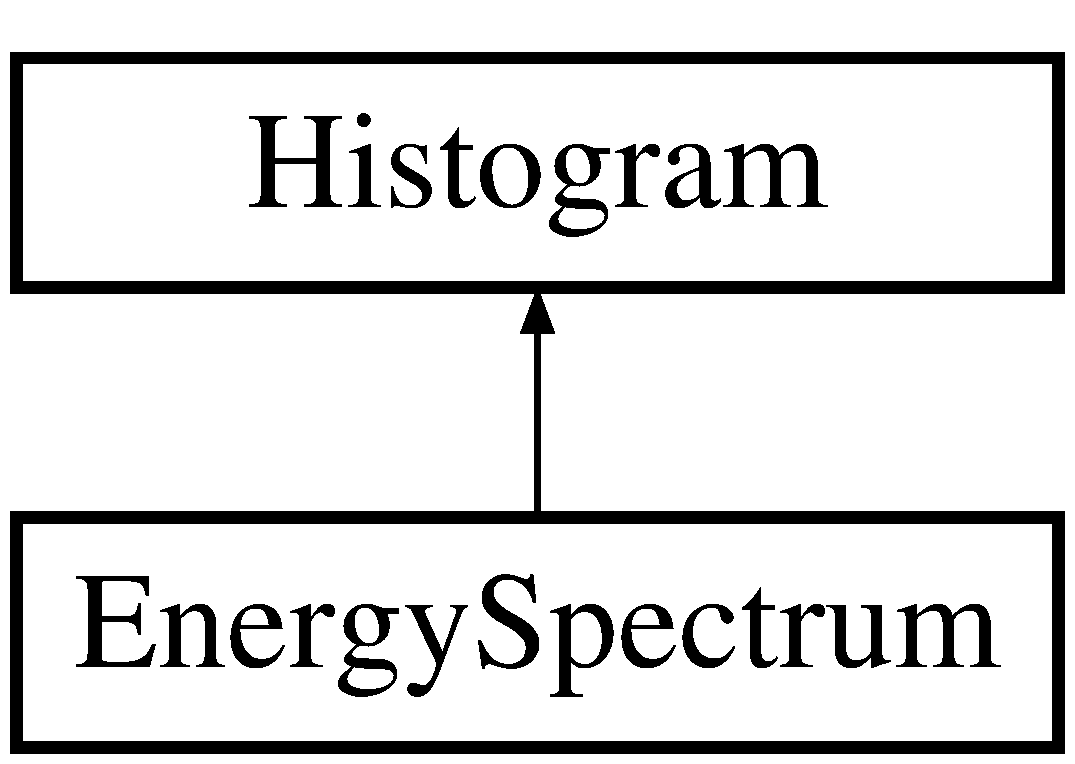
\includegraphics[height=2.000000cm]{classEnergySpectrum}
\end{center}
\end{figure}
\subsubsection*{Public Member Functions}
\begin{DoxyCompactItemize}
\item 
\hypertarget{classEnergySpectrum_a35aa6153b08658999614f041830be69d}{
{\bfseries EnergySpectrum} (\hyperlink{classRunInfo}{RunInfo} \&ri, std::string name)}
\label{classEnergySpectrum_a35aa6153b08658999614f041830be69d}

\end{DoxyCompactItemize}
\subsubsection*{Static Public Attributes}
\begin{DoxyCompactItemize}
\item 
\hypertarget{classEnergySpectrum_a30a91c5193042bf0d2fe353d358d7ca9}{
static const int {\bfseries MIN\_\-COUNTS} = 5}
\label{classEnergySpectrum_a30a91c5193042bf0d2fe353d358d7ca9}

\end{DoxyCompactItemize}


\subsubsection{Detailed Description}
Energy Spectrum 1-\/D histogram class. 

Definition at line 19 of file EnergySpectrum.h.



The documentation for this class was generated from the following file:\begin{DoxyCompactItemize}
\item 
EnergySpectrum.h\end{DoxyCompactItemize}

\hypertarget{classEOFException}{
\subsection{EOFException Class Reference}
\label{classEOFException}\index{EOFException@{EOFException}}
}


Thrown by datareaders when the file is over.  




{\ttfamily \#include $<$Exceptions.h$>$}

Inheritance diagram for EOFException:\begin{figure}[H]
\begin{center}
\leavevmode
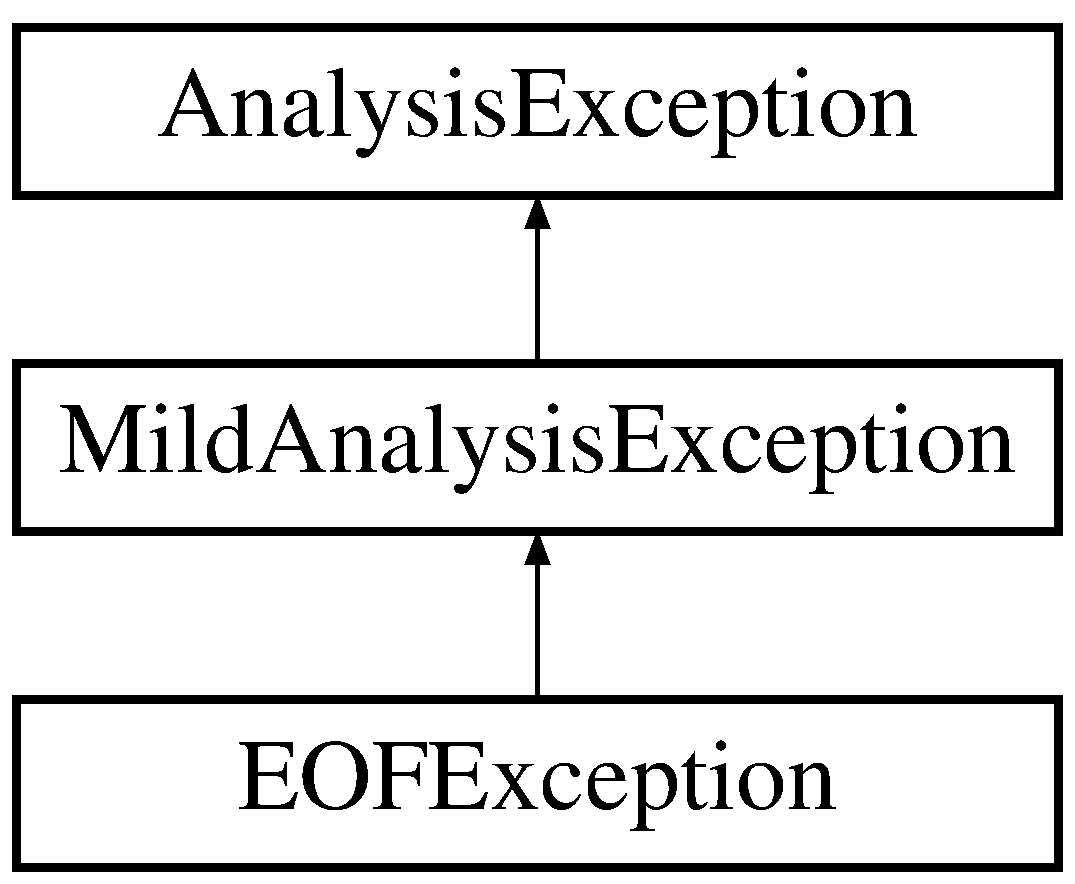
\includegraphics[height=3.000000cm]{classEOFException}
\end{center}
\end{figure}
\subsubsection*{Public Member Functions}
\begin{DoxyCompactItemize}
\item 
\hypertarget{classEOFException_aaa118c24a85b6f76e8fdf400e738ace0}{
{\bfseries EOFException} (const std::string \&str)}
\label{classEOFException_aaa118c24a85b6f76e8fdf400e738ace0}

\end{DoxyCompactItemize}


\subsubsection{Detailed Description}
Thrown by datareaders when the file is over. 

Definition at line 52 of file Exceptions.h.



The documentation for this class was generated from the following file:\begin{DoxyCompactItemize}
\item 
Exceptions.h\end{DoxyCompactItemize}

\hypertarget{structEventRecord}{
\subsection{EventRecord Struct Reference}
\label{structEventRecord}\index{EventRecord@{EventRecord}}
}


Event information.  




{\ttfamily \#include $<$DataRecords.h$>$}

Inheritance diagram for EventRecord:\begin{figure}[H]
\begin{center}
\leavevmode
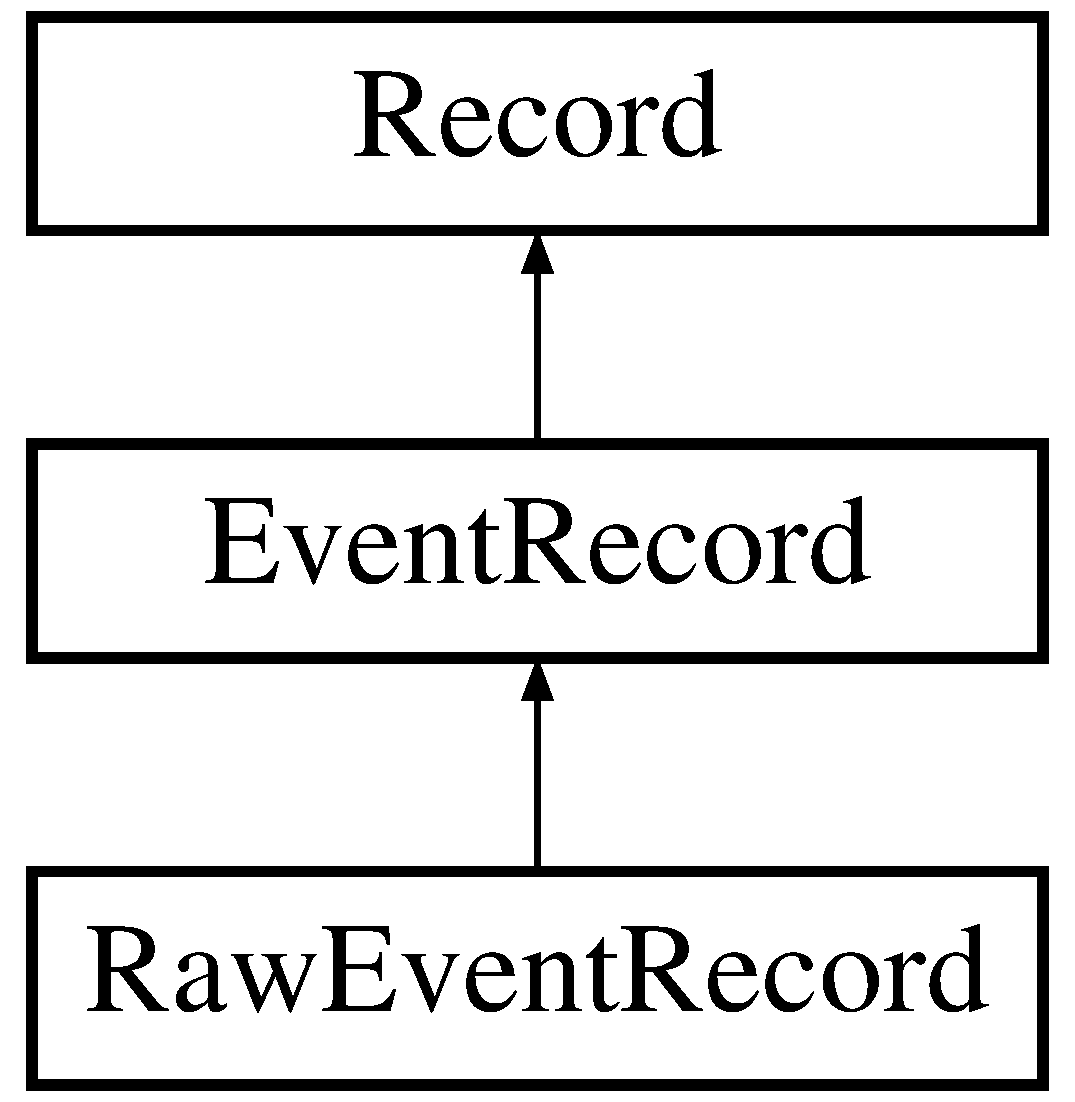
\includegraphics[height=3.000000cm]{structEventRecord}
\end{center}
\end{figure}


\subsubsection{Detailed Description}
Event information. 

Definition at line 58 of file DataRecords.h.



The documentation for this struct was generated from the following file:\begin{DoxyCompactItemize}
\item 
DataRecords.h\end{DoxyCompactItemize}

\hypertarget{classEZCutter}{
\subsection{EZCutter Class Reference}
\label{classEZCutter}\index{EZCutter@{EZCutter}}
}


Extended zenith cutterm Uses SuperCuts-\/like cuts, but with zenith angle corrections based on cos(theta) and 3rd order poly in log(SIZE).  




{\ttfamily \#include $<$EZCutter.h$>$}

Inheritance diagram for EZCutter:\begin{figure}[H]
\begin{center}
\leavevmode
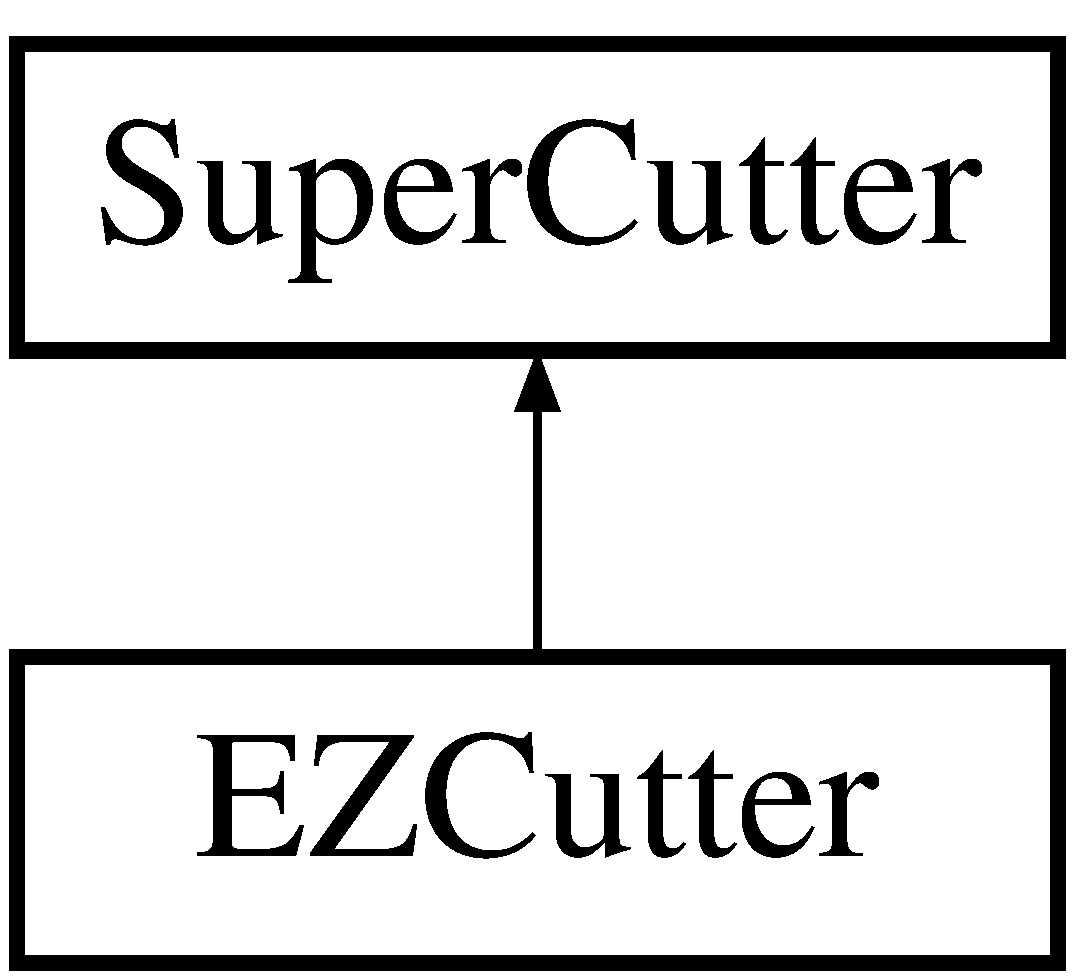
\includegraphics[height=2.000000cm]{classEZCutter}
\end{center}
\end{figure}
\subsubsection*{Public Member Functions}
\begin{DoxyCompactItemize}
\item 
void \hyperlink{classEZCutter_adfef095f257966676350821591df66ed}{applyCorrections} (\hyperlink{structHillasParameterization}{HillasParameterization} \&p)
\item 
\hypertarget{classEZCutter_a2478de078ec3c1e0cf03c40a7cef8ff0}{
void \hyperlink{classEZCutter_a2478de078ec3c1e0cf03c40a7cef8ff0}{setCamera} (int npix, int utdate)}
\label{classEZCutter_a2478de078ec3c1e0cf03c40a7cef8ff0}

\end{DoxyCompactItemize}


\subsubsection{Detailed Description}
Extended zenith cutterm Uses SuperCuts-\/like cuts, but with zenith angle corrections based on cos(theta) and 3rd order poly in log(SIZE). 

Good for spectral cuts. 

Definition at line 13 of file EZCutter.h.



\subsubsection{Member Function Documentation}
\hypertarget{classEZCutter_adfef095f257966676350821591df66ed}{
\index{EZCutter@{EZCutter}!applyCorrections@{applyCorrections}}
\index{applyCorrections@{applyCorrections}!EZCutter@{EZCutter}}
\paragraph[{applyCorrections}]{\setlength{\rightskip}{0pt plus 5cm}void EZCutter::applyCorrections (
\begin{DoxyParamCaption}
\item[{{\bf HillasParameterization} \&}]{param}
\end{DoxyParamCaption}
)\hspace{0.3cm}{\ttfamily  \mbox{[}virtual\mbox{]}}}}
\label{classEZCutter_adfef095f257966676350821591df66ed}


Perform zenith correction. 

Overrides the SuperCutter::prePass() function which is executed before cuts are applied by \hyperlink{classSuperCutter_a10e29b1d569a2b09755e44c31b3c1e61}{SuperCutter::pass()}

\begin{Desc}
\item[\hyperlink{todo__todo000012}{Todo}]: make sigma\_\-pix and the \char`\"{}0.023\char`\"{} free optimization parameters! \end{Desc}


Reimplemented from \hyperlink{classSuperCutter_aa9affeb3c4e8b66860f26bd96954b4e1}{SuperCutter}.



Definition at line 40 of file EZCutter.cpp.



References HillasParameterization::centroid, Camera::getPEToDC(), HillasParameterization::length, HillasParameterization::length\_\-over\_\-size, HillasParameterization::max, HillasParameterization::miss, HillasParameterization::point\_\-of\_\-origin\_\-a, HillasParameterization::point\_\-of\_\-origin\_\-b, HillasParameterization::size, HillasParameterization::width, Coordinate\_\-t::x, Coordinate\_\-t::y, and HillasParameterization::zenith.



The documentation for this class was generated from the following files:\begin{DoxyCompactItemize}
\item 
EZCutter.h\item 
EZCutter.cpp\end{DoxyCompactItemize}

\hypertarget{classFitter}{
\subsection{Fitter Class Reference}
\label{classFitter}\index{Fitter@{Fitter}}
}


Class that performs actual chi-\/square grid search.  




{\ttfamily \#include $<$Fitter.h$>$}

\subsubsection*{Public Member Functions}
\begin{DoxyCompactItemize}
\item 
\hypertarget{classFitter_a23eb026bd4e127cefa0d83e2a6d4f002}{
{\bfseries Fitter} (\hyperlink{classRunInfo}{RunInfo} \&ri)}
\label{classFitter_a23eb026bd4e127cefa0d83e2a6d4f002}

\item 
void \hyperlink{classFitter_a88492ebdbfa181370dc05a584ec9a040}{minimize} (\hyperlink{classEnergySpectrum}{EnergySpectrum} $\ast$energy\_\-on, \hyperlink{classEnergySpectrum}{EnergySpectrum} $\ast$energy\_\-off, double \&N0, double \&Gamma0, double \&e0, double Time, double n0Range, int n0Step, double gRange, int gStep, double onoffratio)
\item 
\hypertarget{classFitter_aeb18a74a610dd87bc662c18ca6c28cc8}{
void \hyperlink{classFitter_aeb18a74a610dd87bc662c18ca6c28cc8}{save} ()}
\label{classFitter_aeb18a74a610dd87bc662c18ca6c28cc8}

\item 
\hypertarget{classFitter_a23eb026bd4e127cefa0d83e2a6d4f002}{
{\bfseries Fitter} (\hyperlink{classRunInfo}{RunInfo} \&ri)}
\label{classFitter_a23eb026bd4e127cefa0d83e2a6d4f002}

\item 
void \hyperlink{classFitter_a6f93aeb7b89a67f368cfa03abdce3e5a}{minimize} (\hyperlink{classEnergySpectrum}{EnergySpectrum} $\ast$energy\_\-on, \hyperlink{classEnergySpectrum}{EnergySpectrum} $\ast$energy\_\-off, double \&N0, double \&Gamma0, double \&E0, double Time, double n0Range, int n0Step, double gRange, int gStep, double e0Range, double e0Step, double onoffratio)
\item 
\hypertarget{classFitter_aeb18a74a610dd87bc662c18ca6c28cc8}{
void {\bfseries save} ()}
\label{classFitter_aeb18a74a610dd87bc662c18ca6c28cc8}

\end{DoxyCompactItemize}


\subsubsection{Detailed Description}
Class that performs actual chi-\/square grid search. 

Definition at line 172 of file Fitter.h.



\subsubsection{Member Function Documentation}
\hypertarget{classFitter_a88492ebdbfa181370dc05a584ec9a040}{
\index{Fitter@{Fitter}!minimize@{minimize}}
\index{minimize@{minimize}!Fitter@{Fitter}}
\paragraph[{minimize}]{\setlength{\rightskip}{0pt plus 5cm}void Fitter::minimize (
\begin{DoxyParamCaption}
\item[{{\bf EnergySpectrum} $\ast$}]{energy\_\-on, }
\item[{{\bf EnergySpectrum} $\ast$}]{energy\_\-off, }
\item[{double \&}]{N0, }
\item[{double \&}]{Gamma0, }
\item[{double \&}]{e0, }
\item[{double}]{Time, }
\item[{double}]{n0Range, }
\item[{int}]{n0Step, }
\item[{double}]{gRange, }
\item[{int}]{gStep, }
\item[{double}]{onoffratio}
\end{DoxyParamCaption}
)}}
\label{classFitter_a88492ebdbfa181370dc05a584ec9a040}


Start Actual Fitting Process Save Chi-\/Square Table in File \char`\"{}Totals/chi.text\char`\"{}. 

\begin{Desc}
\item[\hyperlink{todo__todo000015}{Todo}]: put \char`\"{}alpha\char`\"{} or tracking ratio into the onOff and onOffVariance: onoff = on-\/a$\ast$off, variance=a$\ast$(on+off) or whatever\end{Desc}


Definition at line 333 of file Fitter.cpp.



References Histogram::get(), ProgressBar::print(), and ProgressBar::printClear().

\hypertarget{classFitter_a6f93aeb7b89a67f368cfa03abdce3e5a}{
\index{Fitter@{Fitter}!minimize@{minimize}}
\index{minimize@{minimize}!Fitter@{Fitter}}
\paragraph[{minimize}]{\setlength{\rightskip}{0pt plus 5cm}void Fitter::minimize (
\begin{DoxyParamCaption}
\item[{{\bf EnergySpectrum} $\ast$}]{energy\_\-on, }
\item[{{\bf EnergySpectrum} $\ast$}]{energy\_\-off, }
\item[{double \&}]{N0, }
\item[{double \&}]{Gamma0, }
\item[{double \&}]{E0, }
\item[{double}]{Time, }
\item[{double}]{n0Range, }
\item[{int}]{n0Step, }
\item[{double}]{gRange, }
\item[{int}]{gStep, }
\item[{double}]{e0Range, }
\item[{double}]{e0Step, }
\item[{double}]{onoffratio}
\end{DoxyParamCaption}
)}}
\label{classFitter_a6f93aeb7b89a67f368cfa03abdce3e5a}


Start Actual Fitting Process Save Chi-\/Square Table in File \char`\"{}Totals/chi.text\char`\"{}. 

\begin{Desc}
\item[\hyperlink{todo__todo000018}{Todo}]: put \char`\"{}alpha\char`\"{} or tracking ratio into the onOff and onOffVariance: onoff = on-\/a$\ast$off, variance=a$\ast$(on+off) or whatever\end{Desc}


Definition at line 334 of file FitterNew.cpp.



References Histogram::get(), ProgressBar::print(), and ProgressBar::printClear().



The documentation for this class was generated from the following files:\begin{DoxyCompactItemize}
\item 
Fitter.h\item 
FitterNew.h\item 
Fitter.cpp\item 
FitterNew.cpp\end{DoxyCompactItemize}

\hypertarget{classGainFinder}{
\subsection{GainFinder Class Reference}
\label{classGainFinder}\index{GainFinder@{GainFinder}}
}


Retrieve or calculate nitrogen gains, given a nitrogen run ID.  




{\ttfamily \#include $<$GainFinder.h$>$}

\subsubsection*{Public Member Functions}
\begin{DoxyCompactItemize}
\item 
void \hyperlink{classGainFinder_a093922ed07e211199e2e3afdc4b6b2d4}{getGains} (\hyperlink{classRunInfo}{RunInfo} \&ri, Array\_\-t \&gains, int telescope\_\-id=0)
\item 
void \hyperlink{classGainFinder_a3cd76ff621f0c8fe2113b8fa98a8a45a}{setThresholds} (double, double, double)
\end{DoxyCompactItemize}


\subsubsection{Detailed Description}
Retrieve or calculate nitrogen gains, given a nitrogen run ID. 

Definition at line 14 of file GainFinder.h.



\subsubsection{Member Function Documentation}
\hypertarget{classGainFinder_a093922ed07e211199e2e3afdc4b6b2d4}{
\index{GainFinder@{GainFinder}!getGains@{getGains}}
\index{getGains@{getGains}!GainFinder@{GainFinder}}
\paragraph[{getGains}]{\setlength{\rightskip}{0pt plus 5cm}void GainFinder::getGains (
\begin{DoxyParamCaption}
\item[{{\bf RunInfo} \&}]{ri, }
\item[{Array\_\-t \&}]{gains, }
\item[{int}]{telescope\_\-id = {\ttfamily 0}}
\end{DoxyParamCaption}
)}}
\label{classGainFinder_a093922ed07e211199e2e3afdc4b6b2d4}


Fetch the gains for the specified nitrogen run. 


\begin{DoxyParams}{Parameters}
{\em ri} & -\/ Run information struct from \hyperlink{classConfig}{Config} \\
\hline
{\em id} & -\/ nitrogen gain id \\
\hline
{\em gains} & -\/ uninitialized Array\_\-t where gains will be stored\\
\hline
\end{DoxyParams}
\begin{Desc}
\item[\hyperlink{todo__todo000019}{Todo}]: make gains database have a code column which marks bad gains 

: implement lock file! \end{Desc}


Definition at line 48 of file GainFinder.cpp.



References RunInfo::cachedir, PedestalFinder::getPeds(), RawDataReaderFactory::getReader(), RawDataReaderFactory::instance(), RunInfo::n2id, HeaderRecord::nadc, HeaderRecord::num\_\-telescopes, and PedestalFinder::setTubeOffThresholds().

\hypertarget{classGainFinder_a3cd76ff621f0c8fe2113b8fa98a8a45a}{
\index{GainFinder@{GainFinder}!setThresholds@{setThresholds}}
\index{setThresholds@{setThresholds}!GainFinder@{GainFinder}}
\paragraph[{setThresholds}]{\setlength{\rightskip}{0pt plus 5cm}void GainFinder::setThresholds (
\begin{DoxyParamCaption}
\item[{double}]{min, }
\item[{double}]{max, }
\item[{double}]{percent}
\end{DoxyParamCaption}
)}}
\label{classGainFinder_a3cd76ff621f0c8fe2113b8fa98a8a45a}


Set gain cutoff thresholds. 

The default values are used if this method is not called explicitly. 
\begin{DoxyParams}{Parameters}
{\em min} & -\/ minimim adc value to include in gain calculation (default is 50) \\
\hline
{\em max} & -\/ maximum adc value to include in gain calculation (default 1000) \\
\hline
{\em percent} & -\/ percent of camera above which the image is considered \char`\"{}saturated\char`\"{} and should be ignored for gain calculations (default 0.75) \\
\hline
\end{DoxyParams}


Definition at line 30 of file GainFinder.cpp.



The documentation for this class was generated from the following files:\begin{DoxyCompactItemize}
\item 
GainFinder.h\item 
GainFinder.cpp\end{DoxyCompactItemize}

\hypertarget{classGaussianDeviate}{
\subsection{GaussianDeviate Class Reference}
\label{classGaussianDeviate}\index{GaussianDeviate@{GaussianDeviate}}
}
\subsubsection*{Public Member Functions}
\begin{DoxyCompactItemize}
\item 
\hypertarget{classGaussianDeviate_a654ded9268df74c252c32ea00c8abafa}{
{\bfseries GaussianDeviate} (std::string \&dbdir)}
\label{classGaussianDeviate_a654ded9268df74c252c32ea00c8abafa}

\item 
\hypertarget{classGaussianDeviate_ad98fee7b19ed54a1bb6db1fb8150157e}{
double {\bfseries getDeviate} ()}
\label{classGaussianDeviate_ad98fee7b19ed54a1bb6db1fb8150157e}

\item 
\hypertarget{classGaussianDeviate_a356bb7235f0d7da3330772bc05b389f0}{
double \hyperlink{classGaussianDeviate_a356bb7235f0d7da3330772bc05b389f0}{getFastDeviate} ()}
\label{classGaussianDeviate_a356bb7235f0d7da3330772bc05b389f0}

\end{DoxyCompactItemize}
\subsubsection*{Static Public Attributes}
\begin{DoxyCompactItemize}
\item 
\hypertarget{classGaussianDeviate_a14d3c4e3117ce6c6d37a4cbc264c321a}{
static const int {\bfseries DBSIZE} = 1000000}
\label{classGaussianDeviate_a14d3c4e3117ce6c6d37a4cbc264c321a}

\end{DoxyCompactItemize}


\subsubsection{Detailed Description}


Definition at line 12 of file GaussianDeviate.h.



The documentation for this class was generated from the following files:\begin{DoxyCompactItemize}
\item 
GaussianDeviate.h\item 
GaussianDeviate.cpp\end{DoxyCompactItemize}

\hypertarget{structHeaderRecord}{
\subsection{HeaderRecord Struct Reference}
\label{structHeaderRecord}\index{HeaderRecord@{HeaderRecord}}
}


Run information (header) from raw datafiles.  




{\ttfamily \#include $<$DataRecords.h$>$}

Inheritance diagram for HeaderRecord:\begin{figure}[H]
\begin{center}
\leavevmode
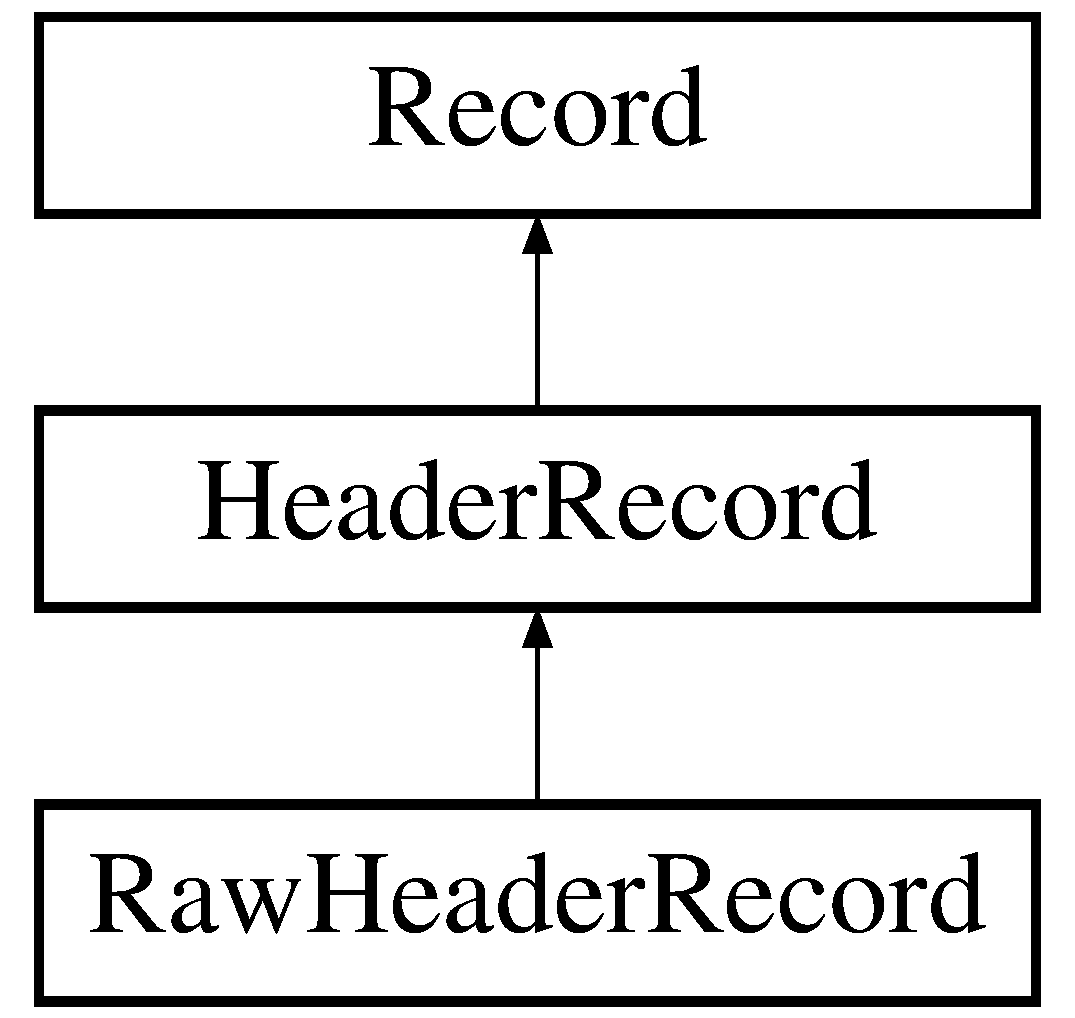
\includegraphics[height=3.000000cm]{structHeaderRecord}
\end{center}
\end{figure}
\subsubsection*{Public Attributes}
\begin{DoxyCompactItemize}
\item 
\hypertarget{structHeaderRecord_a39755fe6ecf64facbd51589bcb66d451}{
int \hyperlink{structHeaderRecord_a39755fe6ecf64facbd51589bcb66d451}{num\_\-telescopes}}
\label{structHeaderRecord_a39755fe6ecf64facbd51589bcb66d451}

\item 
\hypertarget{structHeaderRecord_aa5aaa915ec137ce6510c4ed9802dd713}{
std::vector$<$ int $>$ \hyperlink{structHeaderRecord_aa5aaa915ec137ce6510c4ed9802dd713}{nadc}}
\label{structHeaderRecord_aa5aaa915ec137ce6510c4ed9802dd713}

\item 
\hypertarget{structHeaderRecord_a2f8307833dbe6f23944903cd21ea78b6}{
double \hyperlink{structHeaderRecord_a2f8307833dbe6f23944903cd21ea78b6}{ra}}
\label{structHeaderRecord_a2f8307833dbe6f23944903cd21ea78b6}

\item 
\hypertarget{structHeaderRecord_a85927153a843227a279beac0c4fbd99a}{
double \hyperlink{structHeaderRecord_a85927153a843227a279beac0c4fbd99a}{dec}}
\label{structHeaderRecord_a85927153a843227a279beac0c4fbd99a}

\item 
\hypertarget{structHeaderRecord_ac62dff93f075263fe5b4ba6898821778}{
double \hyperlink{structHeaderRecord_ac62dff93f075263fe5b4ba6898821778}{starttime}}
\label{structHeaderRecord_ac62dff93f075263fe5b4ba6898821778}

\item 
\hypertarget{structHeaderRecord_ae69ec66d5e5904776cb35ea3f8d28729}{
double \hyperlink{structHeaderRecord_ae69ec66d5e5904776cb35ea3f8d28729}{endtime}}
\label{structHeaderRecord_ae69ec66d5e5904776cb35ea3f8d28729}

\item 
\hypertarget{structHeaderRecord_ada2acccb51b80a28f583c987fc72024a}{
double \hyperlink{structHeaderRecord_ada2acccb51b80a28f583c987fc72024a}{average\_\-elevation}}
\label{structHeaderRecord_ada2acccb51b80a28f583c987fc72024a}

\item 
\hypertarget{structHeaderRecord_a7ec95cb209f91d22fc78baeb974bd897}{
int \hyperlink{structHeaderRecord_a7ec95cb209f91d22fc78baeb974bd897}{windowsize}}
\label{structHeaderRecord_a7ec95cb209f91d22fc78baeb974bd897}

\item 
\hypertarget{structHeaderRecord_abe54c31e39ebf8b8b6e642aa9eb1d33e}{
std::string \hyperlink{structHeaderRecord_abe54c31e39ebf8b8b6e642aa9eb1d33e}{sourcename}}
\label{structHeaderRecord_abe54c31e39ebf8b8b6e642aa9eb1d33e}

\end{DoxyCompactItemize}


\subsubsection{Detailed Description}
Run information (header) from raw datafiles. 

\begin{Desc}
\item[\hyperlink{todo__todo000010}{Todo}]: add fields for picture/boundary threshold so they can be checked by wucut -\/ don't want to accidently use cuts which were designed for one threshold after you parameterize with another! \end{Desc}


Definition at line 30 of file DataRecords.h.



The documentation for this struct was generated from the following file:\begin{DoxyCompactItemize}
\item 
DataRecords.h\end{DoxyCompactItemize}

\hypertarget{classHillasImageAnalyzer}{
\subsection{HillasImageAnalyzer Class Reference}
\label{classHillasImageAnalyzer}\index{HillasImageAnalyzer@{HillasImageAnalyzer}}
}


Calculates the Hillas parameters and 2D point of origin of a cleaned image.  




{\ttfamily \#include $<$ImageAnalyzer.h$>$}

Inheritance diagram for HillasImageAnalyzer:\begin{figure}[H]
\begin{center}
\leavevmode
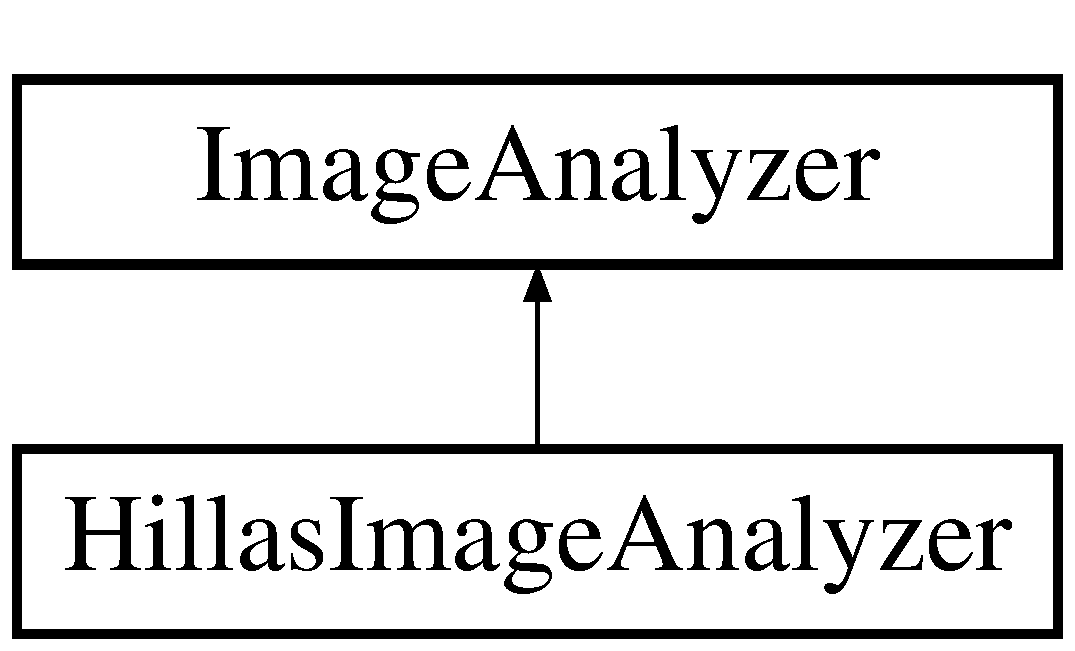
\includegraphics[height=2.000000cm]{classHillasImageAnalyzer}
\end{center}
\end{figure}
\subsubsection*{Public Member Functions}
\begin{DoxyCompactItemize}
\item 
\hyperlink{classHillasImageAnalyzer_aea4e48e8d339197bee6779f342578c1e}{HillasImageAnalyzer} (\hyperlink{classCamera}{Camera} $\ast$cam, double elongation=1.68)
\item 
\hypertarget{classHillasImageAnalyzer_a9b40029788b2d4c8420bc717a684351b}{
void {\bfseries parameterize} (const Array\_\-t \&image, std::vector$<$ int $>$ \&cleanpixels)}
\label{classHillasImageAnalyzer_a9b40029788b2d4c8420bc717a684351b}

\item 
\hypertarget{classHillasImageAnalyzer_a550511668d93263f330835b91ed9736e}{
void {\bfseries setElongationFactor} (double e)}
\label{classHillasImageAnalyzer_a550511668d93263f330835b91ed9736e}

\item 
\hypertarget{classHillasImageAnalyzer_ab9c2f4930a02e6d13d73a136031a97e2}{
\hyperlink{structHillasParameterization}{HillasParameterization} {\bfseries getHillasParameters} ()}
\label{classHillasImageAnalyzer_ab9c2f4930a02e6d13d73a136031a97e2}

\item 
\hypertarget{classHillasImageAnalyzer_a02a2a87a5aedb07989f29a9f2937d59a}{
void {\bfseries enable2D} (bool val=true)}
\label{classHillasImageAnalyzer_a02a2a87a5aedb07989f29a9f2937d59a}

\item 
\hypertarget{classHillasImageAnalyzer_abbc677e62927a5a870b03182d61eb025}{
bool {\bfseries is2DEnabled} ()}
\label{classHillasImageAnalyzer_abbc677e62927a5a870b03182d61eb025}

\end{DoxyCompactItemize}


\subsubsection{Detailed Description}
Calculates the Hillas parameters and 2D point of origin of a cleaned image. 

Definition at line 110 of file ImageAnalyzer.h.



\subsubsection{Constructor \& Destructor Documentation}
\hypertarget{classHillasImageAnalyzer_aea4e48e8d339197bee6779f342578c1e}{
\index{HillasImageAnalyzer@{HillasImageAnalyzer}!HillasImageAnalyzer@{HillasImageAnalyzer}}
\index{HillasImageAnalyzer@{HillasImageAnalyzer}!HillasImageAnalyzer@{HillasImageAnalyzer}}
\paragraph[{HillasImageAnalyzer}]{\setlength{\rightskip}{0pt plus 5cm}HillasImageAnalyzer::HillasImageAnalyzer (
\begin{DoxyParamCaption}
\item[{{\bf Camera} $\ast$}]{cam, }
\item[{double}]{elongation = {\ttfamily 1.68}}
\end{DoxyParamCaption}
)}}
\label{classHillasImageAnalyzer_aea4e48e8d339197bee6779f342578c1e}


Create a new \hyperlink{classHillasImageAnalyzer}{HillasImageAnalyzer} with the camera geometry specified by cam. 


\begin{DoxyParams}{Parameters}
{\em cam} & The \hyperlink{classCamera}{Camera} object that the \hyperlink{classHillasImageAnalyzer}{HillasImageAnalyzer} should use to determine the camera geometry \\
\hline
\end{DoxyParams}


Definition at line 63 of file ImageAnalyzer.cpp.



The documentation for this class was generated from the following files:\begin{DoxyCompactItemize}
\item 
ImageAnalyzer.h\item 
ImageAnalyzer.cpp\end{DoxyCompactItemize}

\hypertarget{structHillasParameterization}{
\subsection{HillasParameterization Struct Reference}
\label{structHillasParameterization}\index{HillasParameterization@{HillasParameterization}}
}


Parameterization of an image, produced by the \hyperlink{classImageAnalyzer}{ImageAnalyzer} object.  




{\ttfamily \#include $<$ImageAnalyzer.h$>$}

Inheritance diagram for HillasParameterization:\begin{figure}[H]
\begin{center}
\leavevmode
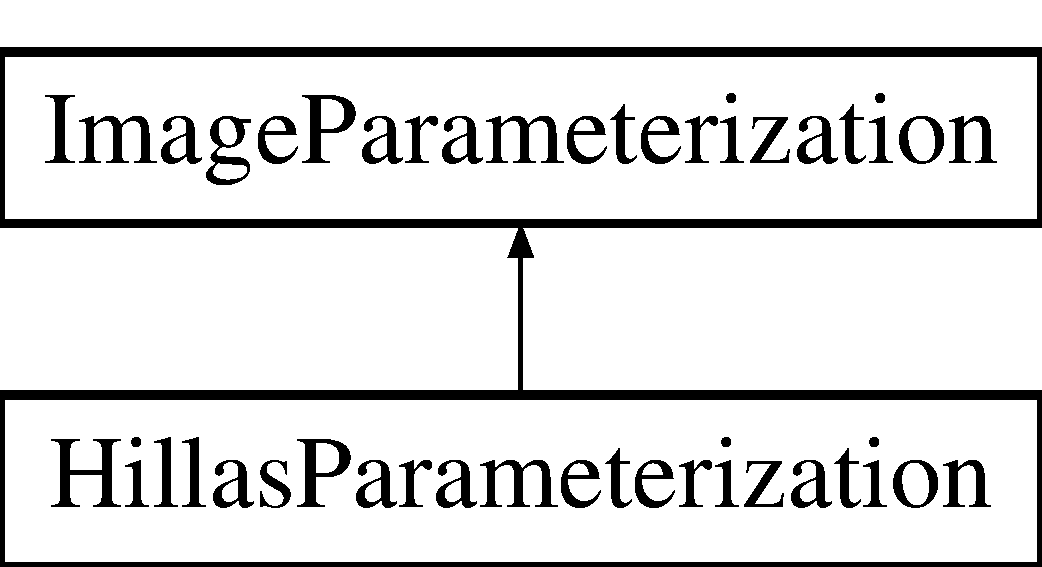
\includegraphics[height=2.000000cm]{structHillasParameterization}
\end{center}
\end{figure}
\subsubsection*{Public Attributes}
\begin{DoxyCompactItemize}
\item 
\hypertarget{structHillasParameterization_ae9b74033dd0e0671e59656a100358d5a}{
\hyperlink{structCoordinate__t}{Coordinate\_\-t} \hyperlink{structHillasParameterization_ae9b74033dd0e0671e59656a100358d5a}{centroid}}
\label{structHillasParameterization_ae9b74033dd0e0671e59656a100358d5a}

\item 
\hypertarget{structHillasParameterization_a32d9137a17d9b447695f50320697e9be}{
\hyperlink{structCoordinate__t}{Coordinate\_\-t} \hyperlink{structHillasParameterization_a32d9137a17d9b447695f50320697e9be}{point\_\-of\_\-origin\_\-a}}
\label{structHillasParameterization_a32d9137a17d9b447695f50320697e9be}

\item 
\hypertarget{structHillasParameterization_a75b3e07788abe724e458ed14aa1339c9}{
\hyperlink{structCoordinate__t}{Coordinate\_\-t} \hyperlink{structHillasParameterization_a75b3e07788abe724e458ed14aa1339c9}{point\_\-of\_\-origin\_\-b}}
\label{structHillasParameterization_a75b3e07788abe724e458ed14aa1339c9}

\item 
\hypertarget{structHillasParameterization_ad2aa423ddc75ba1e108fa31878ed756a}{
double \hyperlink{structHillasParameterization_ad2aa423ddc75ba1e108fa31878ed756a}{length}}
\label{structHillasParameterization_ad2aa423ddc75ba1e108fa31878ed756a}

\item 
\hypertarget{structHillasParameterization_aadb8f3295cbf2b2e0a60c44ede3de8b2}{
double \hyperlink{structHillasParameterization_aadb8f3295cbf2b2e0a60c44ede3de8b2}{width}}
\label{structHillasParameterization_aadb8f3295cbf2b2e0a60c44ede3de8b2}

\item 
\hypertarget{structHillasParameterization_abec8385793292018263164ea18601219}{
double \hyperlink{structHillasParameterization_abec8385793292018263164ea18601219}{size}}
\label{structHillasParameterization_abec8385793292018263164ea18601219}

\item 
\hypertarget{structHillasParameterization_abe4f9cf30a5aaad841297471501889a9}{
double \hyperlink{structHillasParameterization_abe4f9cf30a5aaad841297471501889a9}{miss}}
\label{structHillasParameterization_abe4f9cf30a5aaad841297471501889a9}

\item 
\hypertarget{structHillasParameterization_a3b247cc3ffeeea0972a94f2f6575a5a2}{
double \hyperlink{structHillasParameterization_a3b247cc3ffeeea0972a94f2f6575a5a2}{distance}}
\label{structHillasParameterization_a3b247cc3ffeeea0972a94f2f6575a5a2}

\item 
\hypertarget{structHillasParameterization_a6fc8946c0495cb35f4417e9afbabdce0}{
double \hyperlink{structHillasParameterization_a6fc8946c0495cb35f4417e9afbabdce0}{azwidth}}
\label{structHillasParameterization_a6fc8946c0495cb35f4417e9afbabdce0}

\item 
\hypertarget{structHillasParameterization_a1e908584f4dc7d52c573608b996c86cc}{
double \hyperlink{structHillasParameterization_a1e908584f4dc7d52c573608b996c86cc}{alpha}}
\label{structHillasParameterization_a1e908584f4dc7d52c573608b996c86cc}

\item 
\hypertarget{structHillasParameterization_a2be5e9e0885f119cf5df38aa77777542}{
double \hyperlink{structHillasParameterization_a2be5e9e0885f119cf5df38aa77777542}{length\_\-over\_\-size}}
\label{structHillasParameterization_a2be5e9e0885f119cf5df38aa77777542}

\item 
\hypertarget{structHillasParameterization_ad01c2f44c100dbc06ca180f93bcfae80}{
double \hyperlink{structHillasParameterization_ad01c2f44c100dbc06ca180f93bcfae80}{psi}}
\label{structHillasParameterization_ad01c2f44c100dbc06ca180f93bcfae80}

\item 
\hypertarget{structHillasParameterization_a0592a9cf31f63ed2a19ae4022056981c}{
double \hyperlink{structHillasParameterization_a0592a9cf31f63ed2a19ae4022056981c}{phi}}
\label{structHillasParameterization_a0592a9cf31f63ed2a19ae4022056981c}

\item 
\hypertarget{structHillasParameterization_a7d8e7d294ee5e6dc185257c9e1adb994}{
double \hyperlink{structHillasParameterization_a7d8e7d294ee5e6dc185257c9e1adb994}{max} \mbox{[}3\mbox{]}}
\label{structHillasParameterization_a7d8e7d294ee5e6dc185257c9e1adb994}

\item 
\hypertarget{structHillasParameterization_a92be23975c7807174d8cb4cf32ed07de}{
int \hyperlink{structHillasParameterization_a92be23975c7807174d8cb4cf32ed07de}{index\_\-of\_\-max} \mbox{[}3\mbox{]}}
\label{structHillasParameterization_a92be23975c7807174d8cb4cf32ed07de}

\item 
\hypertarget{structHillasParameterization_acd0f28b7341a288c0aec029f85610247}{
double \hyperlink{structHillasParameterization_acd0f28b7341a288c0aec029f85610247}{frac} \mbox{[}3\mbox{]}}
\label{structHillasParameterization_acd0f28b7341a288c0aec029f85610247}

\item 
\hypertarget{structHillasParameterization_a973a0f8fbe33182e15cf8d585dba5657}{
int \hyperlink{structHillasParameterization_a973a0f8fbe33182e15cf8d585dba5657}{pixels\_\-in\_\-picture}}
\label{structHillasParameterization_a973a0f8fbe33182e15cf8d585dba5657}

\item 
\hypertarget{structHillasParameterization_aefb1906b72858ad355eac40bfc0f313b}{
double \hyperlink{structHillasParameterization_aefb1906b72858ad355eac40bfc0f313b}{asymmetry}}
\label{structHillasParameterization_aefb1906b72858ad355eac40bfc0f313b}

\item 
\hypertarget{structHillasParameterization_a8a07467067d17d6430677bcae47b3c58}{
int \hyperlink{structHillasParameterization_a8a07467067d17d6430677bcae47b3c58}{on}}
\label{structHillasParameterization_a8a07467067d17d6430677bcae47b3c58}

\item 
\hypertarget{structHillasParameterization_aa9e06ca0a327df412ce4b314e0e8a093}{
double \hyperlink{structHillasParameterization_aa9e06ca0a327df412ce4b314e0e8a093}{zenith}}
\label{structHillasParameterization_aa9e06ca0a327df412ce4b314e0e8a093}

\item 
\hypertarget{structHillasParameterization_aaa67bb030d146dca24a4ef045b4ad1d2}{
double \hyperlink{structHillasParameterization_aaa67bb030d146dca24a4ef045b4ad1d2}{energy\_\-estimate}}
\label{structHillasParameterization_aaa67bb030d146dca24a4ef045b4ad1d2}

\end{DoxyCompactItemize}
\subsubsection*{Friends}
\begin{DoxyCompactItemize}
\item 
\hypertarget{structHillasParameterization_a2a0dbb088d9df8f10a6ac85f171cdab0}{
std::ostream \& {\bfseries operator$<$$<$} (std::ostream \&stream, const \hyperlink{structHillasParameterization}{HillasParameterization} \&p)}
\label{structHillasParameterization_a2a0dbb088d9df8f10a6ac85f171cdab0}

\end{DoxyCompactItemize}


\subsubsection{Detailed Description}
Parameterization of an image, produced by the \hyperlink{classImageAnalyzer}{ImageAnalyzer} object. 

I kept this a pure struct, not a class so that the gsl N-\/tuple routines can process it. 

Definition at line 37 of file ImageAnalyzer.h.



The documentation for this struct was generated from the following file:\begin{DoxyCompactItemize}
\item 
ImageAnalyzer.h\end{DoxyCompactItemize}

\hypertarget{classHistogram}{
\subsection{Histogram Class Reference}
\label{classHistogram}\index{Histogram@{Histogram}}
}


General 1-\/D histogram class.  




{\ttfamily \#include $<$Histogram.h$>$}

Inheritance diagram for Histogram:\begin{figure}[H]
\begin{center}
\leavevmode
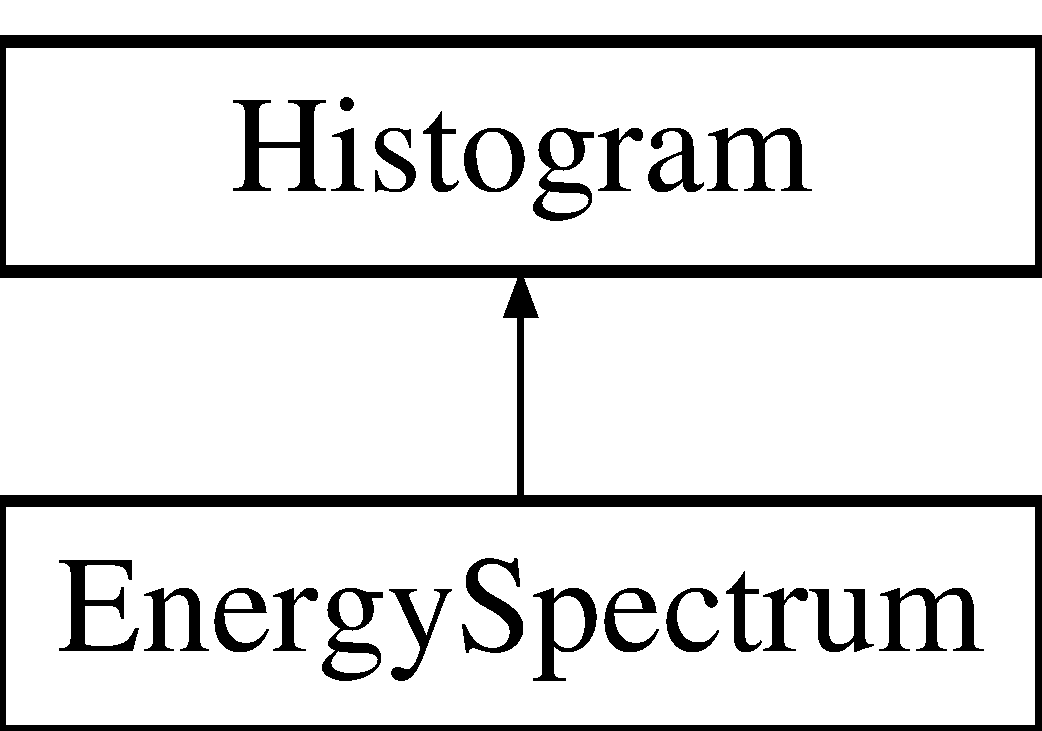
\includegraphics[height=2.000000cm]{classHistogram}
\end{center}
\end{figure}
\subsubsection*{Public Member Functions}
\begin{DoxyCompactItemize}
\item 
\hyperlink{classHistogram_a0e67c772215a44412bea53d7c42a9afd}{Histogram} (int, double, double, std::string)
\item 
\hyperlink{classHistogram_a57bd7d0018ca67ebc964a70856a45121}{Histogram} (const \hyperlink{classHistogram}{Histogram} \&h)
\item 
void \hyperlink{classHistogram_aeb18a84d7511ee5955ce41c2e566ed42}{increment} (double)
\item 
\hypertarget{classHistogram_ac071a756a6a7e7b762e54d40a3b063d2}{
void \hyperlink{classHistogram_ac071a756a6a7e7b762e54d40a3b063d2}{accumulate} (double x, double weight)}
\label{classHistogram_ac071a756a6a7e7b762e54d40a3b063d2}

\item 
\hypertarget{classHistogram_a1adaf843802a7dd123aa3d981a3fe40a}{
int \hyperlink{classHistogram_a1adaf843802a7dd123aa3d981a3fe40a}{maxBin} ()}
\label{classHistogram_a1adaf843802a7dd123aa3d981a3fe40a}

\item 
\hypertarget{classHistogram_ad8f309ad710edf09dd5b5f5212fea317}{
int \hyperlink{classHistogram_ad8f309ad710edf09dd5b5f5212fea317}{minBin} ()}
\label{classHistogram_ad8f309ad710edf09dd5b5f5212fea317}

\item 
\hypertarget{classHistogram_ab03071830f982d65161093f6e21d337b}{
double \hyperlink{classHistogram_ab03071830f982d65161093f6e21d337b}{maxValue} ()}
\label{classHistogram_ab03071830f982d65161093f6e21d337b}

\item 
\hypertarget{classHistogram_aa542bc0d079c028891332f075e36de6d}{
double \hyperlink{classHistogram_aa542bc0d079c028891332f075e36de6d}{minValue} ()}
\label{classHistogram_aa542bc0d079c028891332f075e36de6d}

\item 
\hypertarget{classHistogram_a232fa623a8fb507ce61f3d4d887261c4}{
void \hyperlink{classHistogram_a232fa623a8fb507ce61f3d4d887261c4}{getRange} (int bin, double \&lower, double \&upper)}
\label{classHistogram_a232fa623a8fb507ce61f3d4d887261c4}

\item 
double \hyperlink{classHistogram_a60aec75a406846e8ddfcb5cd3bfd08b6}{mean} ()
\item 
double \hyperlink{classHistogram_ace6b4ef16828ca568a9ffb6195f2f85a}{sigma} ()
\item 
double \hyperlink{classHistogram_a66f96b43325ad5daef6c208706cb8116}{sum} ()
\item 
\hypertarget{classHistogram_a503db836fe4146f1978433ceb44fbfd5}{
void {\bfseries save} (std::string)}
\label{classHistogram_a503db836fe4146f1978433ceb44fbfd5}

\item 
void \hyperlink{classHistogram_aec3e06fe7bbbd75cf0b3a2c9e44da2df}{load} (std::string)
\item 
int \hyperlink{classHistogram_a7f7a8382c6450c8b2f58644d569350fe}{findBinWithValue} (double val)
\item 
void \hyperlink{classHistogram_a3f1ace79184ce1eb65b08d7cef9c3ef7}{saveStatistics} (std::string)
\item 
\hypertarget{classHistogram_ad841b25d1f867051f99539bfe88b0dc1}{
int {\bfseries numBins} ()}
\label{classHistogram_ad841b25d1f867051f99539bfe88b0dc1}

\item 
\hypertarget{classHistogram_ad63d2457f4c475441626169ac47c6280}{
void \hyperlink{classHistogram_ad63d2457f4c475441626169ac47c6280}{scale} (double val)}
\label{classHistogram_ad63d2457f4c475441626169ac47c6280}

\item 
void \hyperlink{classHistogram_a2714fcfb141d09432600fc8e6c65d3f3}{subtract} (\hyperlink{classHistogram}{Histogram} \&h)
\item 
\hypertarget{classHistogram_a60716135cdc3419f91875f0d89e03a9a}{
double \hyperlink{classHistogram_a60716135cdc3419f91875f0d89e03a9a}{operator\mbox{[}$\,$\mbox{]}} (int)}
\label{classHistogram_a60716135cdc3419f91875f0d89e03a9a}

\item 
double \hyperlink{classHistogram_ab93e201f4b23def54a4ce5fda5c9d085}{get} (int bin)
\item 
\hypertarget{classHistogram_ab18fbea2f675c873c9c90d60eaf5dd28}{
void \hyperlink{classHistogram_ab18fbea2f675c873c9c90d60eaf5dd28}{reset} ()}
\label{classHistogram_ab18fbea2f675c873c9c90d60eaf5dd28}

\item 
\hypertarget{classHistogram_aa8efafbdf6c0f5c927c32fa4e132767c}{
gsl\_\-histogram $\ast$ {\bfseries getGSLHist} ()}
\label{classHistogram_aa8efafbdf6c0f5c927c32fa4e132767c}

\end{DoxyCompactItemize}


\subsubsection{Detailed Description}
General 1-\/D histogram class. 

\begin{Desc}
\item[\hyperlink{todo__todo000020}{Todo}]: Make this class work with lightcurve data where the first and last bins may be partially filled (or smaller width) \end{Desc}


Definition at line 21 of file Histogram.h.



\subsubsection{Constructor \& Destructor Documentation}
\hypertarget{classHistogram_a0e67c772215a44412bea53d7c42a9afd}{
\index{Histogram@{Histogram}!Histogram@{Histogram}}
\index{Histogram@{Histogram}!Histogram@{Histogram}}
\paragraph[{Histogram}]{\setlength{\rightskip}{0pt plus 5cm}Histogram::Histogram (
\begin{DoxyParamCaption}
\item[{int}]{nbins, }
\item[{double}]{minx, }
\item[{double}]{maxx, }
\item[{std::string}]{name}
\end{DoxyParamCaption}
)}}
\label{classHistogram_a0e67c772215a44412bea53d7c42a9afd}


Create a new \hyperlink{classHistogram}{Histogram}. 


\begin{DoxyParams}{Parameters}
{\em numbins} & number of bins \\
\hline
{\em min} & minimum value \\
\hline
{\em max} & maximum value \\
\hline
{\em name} & description of the histogram \\
\hline
\end{DoxyParams}


Definition at line 34 of file Histogram.cpp.

\hypertarget{classHistogram_a57bd7d0018ca67ebc964a70856a45121}{
\index{Histogram@{Histogram}!Histogram@{Histogram}}
\index{Histogram@{Histogram}!Histogram@{Histogram}}
\paragraph[{Histogram}]{\setlength{\rightskip}{0pt plus 5cm}Histogram::Histogram (
\begin{DoxyParamCaption}
\item[{const {\bf Histogram} \&}]{h}
\end{DoxyParamCaption}
)}}
\label{classHistogram_a57bd7d0018ca67ebc964a70856a45121}


Copy constructor. 

\begin{Desc}
\item[\hyperlink{bug__bug000002}{Bug}]: doesn't work yet \end{Desc}


Definition at line 71 of file Histogram.cpp.



\subsubsection{Member Function Documentation}
\hypertarget{classHistogram_a7f7a8382c6450c8b2f58644d569350fe}{
\index{Histogram@{Histogram}!findBinWithValue@{findBinWithValue}}
\index{findBinWithValue@{findBinWithValue}!Histogram@{Histogram}}
\paragraph[{findBinWithValue}]{\setlength{\rightskip}{0pt plus 5cm}int Histogram::findBinWithValue (
\begin{DoxyParamCaption}
\item[{double}]{val}
\end{DoxyParamCaption}
)}}
\label{classHistogram_a7f7a8382c6450c8b2f58644d569350fe}
\begin{DoxyReturn}{Returns}
index of bin with the specified value, -\/1 on failure. 
\end{DoxyReturn}


Definition at line 351 of file Histogram.cpp.

\hypertarget{classHistogram_ab93e201f4b23def54a4ce5fda5c9d085}{
\index{Histogram@{Histogram}!get@{get}}
\index{get@{get}!Histogram@{Histogram}}
\paragraph[{get}]{\setlength{\rightskip}{0pt plus 5cm}double Histogram::get (
\begin{DoxyParamCaption}
\item[{int}]{i}
\end{DoxyParamCaption}
)\hspace{0.3cm}{\ttfamily  \mbox{[}inline\mbox{]}}}}
\label{classHistogram_ab93e201f4b23def54a4ce5fda5c9d085}


Return histogram value at index i. 

Can also use the \mbox{[}\mbox{]} operator (i.e. myhist\mbox{[}3\mbox{]} is equivalent to myhist.get(3)) 

Definition at line 108 of file Histogram.h.



Referenced by Fitter::minimize().

\hypertarget{classHistogram_aeb18a84d7511ee5955ce41c2e566ed42}{
\index{Histogram@{Histogram}!increment@{increment}}
\index{increment@{increment}!Histogram@{Histogram}}
\paragraph[{increment}]{\setlength{\rightskip}{0pt plus 5cm}void Histogram::increment (
\begin{DoxyParamCaption}
\item[{double}]{x}
\end{DoxyParamCaption}
)\hspace{0.3cm}{\ttfamily  \mbox{[}inline\mbox{]}}}}
\label{classHistogram_aeb18a84d7511ee5955ce41c2e566ed42}


Increment the bin corresponding to the specified value. 

Implemented as an inline function for speed. 

Definition at line 70 of file Histogram.h.



References maxValue(), and minValue().



Referenced by WUArray::analyzeRun(), and Cutter::cut().

\hypertarget{classHistogram_aec3e06fe7bbbd75cf0b3a2c9e44da2df}{
\index{Histogram@{Histogram}!load@{load}}
\index{load@{load}!Histogram@{Histogram}}
\paragraph[{load}]{\setlength{\rightskip}{0pt plus 5cm}void Histogram::load (
\begin{DoxyParamCaption}
\item[{std::string}]{filename}
\end{DoxyParamCaption}
)}}
\label{classHistogram_aec3e06fe7bbbd75cf0b3a2c9e44da2df}


Read in a histogram saved with the \char`\"{}save\char`\"{} function. 

The histogram to be read must have the number of bins as the \hyperlink{classHistogram}{Histogram} object. 

Definition at line 235 of file Histogram.cpp.

\hypertarget{classHistogram_a60aec75a406846e8ddfcb5cd3bfd08b6}{
\index{Histogram@{Histogram}!mean@{mean}}
\index{mean@{mean}!Histogram@{Histogram}}
\paragraph[{mean}]{\setlength{\rightskip}{0pt plus 5cm}double Histogram::mean (
\begin{DoxyParamCaption}
{}
\end{DoxyParamCaption}
)}}
\label{classHistogram_a60aec75a406846e8ddfcb5cd3bfd08b6}
\begin{DoxyReturn}{Returns}
the mean value in the histogram. 
\end{DoxyReturn}


Definition at line 320 of file Histogram.cpp.



Referenced by saveStatistics().

\hypertarget{classHistogram_a3f1ace79184ce1eb65b08d7cef9c3ef7}{
\index{Histogram@{Histogram}!saveStatistics@{saveStatistics}}
\index{saveStatistics@{saveStatistics}!Histogram@{Histogram}}
\paragraph[{saveStatistics}]{\setlength{\rightskip}{0pt plus 5cm}void Histogram::saveStatistics (
\begin{DoxyParamCaption}
\item[{std::string}]{}
\end{DoxyParamCaption}
)}}
\label{classHistogram_a3f1ace79184ce1eb65b08d7cef9c3ef7}


Write out a text file with statistical info about the histogram. 

This function is automatically called when Histogram::save() is called, but is provided separately in case one wants to just write statistics and not the whole histogram. It would be cleaner to append this to the top of the histogram file itself, but that would make it harder for external programs to read the histogram files, so I decided to keep the stats file separate.


\begin{DoxyParams}{Parameters}
{\em basename} & base filename (.hist.stats is appended) \\
\hline
\end{DoxyParams}


Definition at line 205 of file Histogram.cpp.



References maxBin(), maxValue(), mean(), minBin(), minValue(), sigma(), and sum().



Referenced by Image2D::save().

\hypertarget{classHistogram_ace6b4ef16828ca568a9ffb6195f2f85a}{
\index{Histogram@{Histogram}!sigma@{sigma}}
\index{sigma@{sigma}!Histogram@{Histogram}}
\paragraph[{sigma}]{\setlength{\rightskip}{0pt plus 5cm}double Histogram::sigma (
\begin{DoxyParamCaption}
{}
\end{DoxyParamCaption}
)}}
\label{classHistogram_ace6b4ef16828ca568a9ffb6195f2f85a}
\begin{DoxyReturn}{Returns}
the variance in the histogrammed value. 
\end{DoxyReturn}


Definition at line 330 of file Histogram.cpp.



Referenced by saveStatistics().

\hypertarget{classHistogram_a2714fcfb141d09432600fc8e6c65d3f3}{
\index{Histogram@{Histogram}!subtract@{subtract}}
\index{subtract@{subtract}!Histogram@{Histogram}}
\paragraph[{subtract}]{\setlength{\rightskip}{0pt plus 5cm}void Histogram::subtract (
\begin{DoxyParamCaption}
\item[{{\bf Histogram} \&}]{hist}
\end{DoxyParamCaption}
)}}
\label{classHistogram_a2714fcfb141d09432600fc8e6c65d3f3}


Subtracts the specified histogram from the current one. 


\begin{DoxyParams}{Parameters}
{\em hist} & histogram containing values to subtract. Must have identical bin ranges as the current histogram. \\
\hline
\end{DoxyParams}


Definition at line 386 of file Histogram.cpp.

\hypertarget{classHistogram_a66f96b43325ad5daef6c208706cb8116}{
\index{Histogram@{Histogram}!sum@{sum}}
\index{sum@{sum}!Histogram@{Histogram}}
\paragraph[{sum}]{\setlength{\rightskip}{0pt plus 5cm}double Histogram::sum (
\begin{DoxyParamCaption}
{}
\end{DoxyParamCaption}
)}}
\label{classHistogram_a66f96b43325ad5daef6c208706cb8116}
\begin{DoxyReturn}{Returns}
the total number of counts in the histogram. 
\end{DoxyReturn}


Definition at line 340 of file Histogram.cpp.



Referenced by saveStatistics().



The documentation for this class was generated from the following files:\begin{DoxyCompactItemize}
\item 
Histogram.h\item 
Histogram.cpp\end{DoxyCompactItemize}

\hypertarget{classImage2D}{
\subsection{Image2D Class Reference}
\label{classImage2D}\index{Image2D@{Image2D}}
}


Representation of a 2-\/D raster image (for 2D analysis)  




{\ttfamily \#include $<$Image2D.h$>$}

\subsubsection*{Public Member Functions}
\begin{DoxyCompactItemize}
\item 
\hypertarget{classImage2D_a833d693009805f605c8af82d3acec2af}{
{\bfseries Image2D} (int nxbins=39, int nybins=39)}
\label{classImage2D_a833d693009805f605c8af82d3acec2af}

\item 
void \hyperlink{classImage2D_a9b7675f5771a5f4a0f28a5a7772326a0}{setCoordinateBox} (double minx, double miny, double maxx, double maxy)
\item 
\hypertarget{classImage2D_a4daa00c772ba3c6cdbc678fa1ea555d6}{
double {\bfseries getXCoord} (int i)}
\label{classImage2D_a4daa00c772ba3c6cdbc678fa1ea555d6}

\item 
\hypertarget{classImage2D_a3b100d51fdebe1ba7a2987a5d25db71d}{
double {\bfseries getYCoord} (int j)}
\label{classImage2D_a3b100d51fdebe1ba7a2987a5d25db71d}

\item 
\hypertarget{classImage2D_a347193432850999a7704d373841bfe90}{
double {\bfseries getMinX} ()}
\label{classImage2D_a347193432850999a7704d373841bfe90}

\item 
\hypertarget{classImage2D_a5676662e3538d6fea5dfc61d5a5e4140}{
double {\bfseries getMinY} ()}
\label{classImage2D_a5676662e3538d6fea5dfc61d5a5e4140}

\item 
\hypertarget{classImage2D_aeea76c05c63754d99edb452616911185}{
double {\bfseries getMaxX} ()}
\label{classImage2D_aeea76c05c63754d99edb452616911185}

\item 
\hypertarget{classImage2D_a3918d1ddbe2ca3a282268ef8abc0c003}{
double {\bfseries getMaxY} ()}
\label{classImage2D_a3918d1ddbe2ca3a282268ef8abc0c003}

\item 
\hypertarget{classImage2D_afe3cf97c37486e56e49adcf44dd10d3a}{
void {\bfseries load} (std::string filename)}
\label{classImage2D_afe3cf97c37486e56e49adcf44dd10d3a}

\item 
void \hyperlink{classImage2D_a701ac83af425942beb093fff80880b04}{save} (std::string filename)
\item 
\hypertarget{classImage2D_ad6f25f96ba0f4b0e480995a83e9c6919}{
void \hyperlink{classImage2D_ad6f25f96ba0f4b0e480995a83e9c6919}{savePGM} (std::string filename)}
\label{classImage2D_ad6f25f96ba0f4b0e480995a83e9c6919}

\item 
\hypertarget{classImage2D_a1951a4240aba5293c7f2879b4243c590}{
void \hyperlink{classImage2D_a1951a4240aba5293c7f2879b4243c590}{saveGrid} (std::string filename)}
\label{classImage2D_a1951a4240aba5293c7f2879b4243c590}

\item 
\hypertarget{classImage2D_aec45f19b3ba3256cac22a321179cb5d9}{
void \hyperlink{classImage2D_aec45f19b3ba3256cac22a321179cb5d9}{clear} ()}
\label{classImage2D_aec45f19b3ba3256cac22a321179cb5d9}

\item 
\hypertarget{classImage2D_a567f81e75a048d7659f66563af9bad2b}{
void {\bfseries setPixel} (int i, int j, double val)}
\label{classImage2D_a567f81e75a048d7659f66563af9bad2b}

\item 
\hypertarget{classImage2D_a03cfaa176ee51e6663196f8a120a24a8}{
double {\bfseries getPixel} (int i, int j)}
\label{classImage2D_a03cfaa176ee51e6663196f8a120a24a8}

\item 
\hypertarget{classImage2D_a523442590845b45974b1987f24d97c14}{
void {\bfseries addToPixel} (int i, int j, double val)}
\label{classImage2D_a523442590845b45974b1987f24d97c14}

\item 
void \hyperlink{classImage2D_a1373c4a48a3393f3dc8b0a6382ae0990}{addHist} (double x, double y, double val)
\item 
void \hyperlink{classImage2D_afa47c6e966ae69c72bb58e97f1e58858}{addHistRadially} (double x, double y, double val, float radius)
\item 
\hypertarget{classImage2D_acdf9aed4054987b922b3de8e3aa22b72}{
int {\bfseries getOutsideHits} ()}
\label{classImage2D_acdf9aed4054987b922b3de8e3aa22b72}

\item 
void \hyperlink{classImage2D_a2db2c30389b3e52c8246295989e53755}{addImage} (\hyperlink{classImage2D}{Image2D} \&im)
\item 
\hypertarget{classImage2D_ab41e685b8dff0710d85ea51d9bd748c1}{
void \hyperlink{classImage2D_ab41e685b8dff0710d85ea51d9bd748c1}{applyRadialSmoothing} (double r)}
\label{classImage2D_ab41e685b8dff0710d85ea51d9bd748c1}

\item 
\hypertarget{classImage2D_aedea813aff3d0c8583ec9fed1660c3f0}{
int {\bfseries getXDim} ()}
\label{classImage2D_aedea813aff3d0c8583ec9fed1660c3f0}

\item 
\hypertarget{classImage2D_a56e8c4066142765cefbae500b32b7ec5}{
int {\bfseries getYDim} ()}
\label{classImage2D_a56e8c4066142765cefbae500b32b7ec5}

\item 
\hypertarget{classImage2D_a30ac7fec10d7cca8e57ded1023f9134d}{
double {\bfseries minValue} ()}
\label{classImage2D_a30ac7fec10d7cca8e57ded1023f9134d}

\item 
\hypertarget{classImage2D_ab4831e847a315849ce29b16b579f1be0}{
double {\bfseries maxValue} ()}
\label{classImage2D_ab4831e847a315849ce29b16b579f1be0}

\item 
\hypertarget{classImage2D_ad61b4f34f9750c50b1f52c9905ec4127}{
void \hyperlink{classImage2D_ad61b4f34f9750c50b1f52c9905ec4127}{getIndexOfMax} (int \&i, int \&j)}
\label{classImage2D_ad61b4f34f9750c50b1f52c9905ec4127}

\item 
\hypertarget{classImage2D_a7b9b44ca053ab7c6ceac862409c101df}{
void \hyperlink{classImage2D_a7b9b44ca053ab7c6ceac862409c101df}{expand} ()}
\label{classImage2D_a7b9b44ca053ab7c6ceac862409c101df}

\item 
\hyperlink{classImage2D}{Image2D} $\ast$ \hyperlink{classImage2D_ac0bf085a54600d658f594cadb5069691}{crossCorrelateWith} (\hyperlink{classImage2D}{Image2D} \&)
\item 
\hypertarget{classImage2D_a8106dc5bd861ce8086d9cef69165d282}{
int {\bfseries getXHistBinOf} (double x)}
\label{classImage2D_a8106dc5bd861ce8086d9cef69165d282}

\item 
\hypertarget{classImage2D_a88624daa79e7a7f9ae674b6b880df08b}{
int {\bfseries getYHistBinOf} (double y)}
\label{classImage2D_a88624daa79e7a7f9ae674b6b880df08b}

\end{DoxyCompactItemize}


\subsubsection{Detailed Description}
Representation of a 2-\/D raster image (for 2D analysis) 

Definition at line 14 of file Image2D.h.



\subsubsection{Member Function Documentation}
\hypertarget{classImage2D_a1373c4a48a3393f3dc8b0a6382ae0990}{
\index{Image2D@{Image2D}!addHist@{addHist}}
\index{addHist@{addHist}!Image2D@{Image2D}}
\paragraph[{addHist}]{\setlength{\rightskip}{0pt plus 5cm}void Image2D::addHist (
\begin{DoxyParamCaption}
\item[{double}]{x, }
\item[{double}]{y, }
\item[{double}]{val}
\end{DoxyParamCaption}
)}}
\label{classImage2D_a1373c4a48a3393f3dc8b0a6382ae0990}


Add the specified value to the pixel which contains the coordinate (x,y). 

This is useful for histogramming in 2-\/D. 

Definition at line 104 of file Image2D.cpp.



Referenced by Cutter::cut().

\hypertarget{classImage2D_afa47c6e966ae69c72bb58e97f1e58858}{
\index{Image2D@{Image2D}!addHistRadially@{addHistRadially}}
\index{addHistRadially@{addHistRadially}!Image2D@{Image2D}}
\paragraph[{addHistRadially}]{\setlength{\rightskip}{0pt plus 5cm}void Image2D::addHistRadially (
\begin{DoxyParamCaption}
\item[{double}]{x, }
\item[{double}]{y, }
\item[{double}]{val, }
\item[{float}]{radius}
\end{DoxyParamCaption}
)}}
\label{classImage2D_afa47c6e966ae69c72bb58e97f1e58858}


Adds the value val to all pixels in the image that are within radius of the point (x,y). 

This provides another method to radially smooth an image while filling it. It's slower than calling \hyperlink{classImage2D_ab41e685b8dff0710d85ea51d9bd748c1}{applyRadialSmoothing()} after an image has been created, but it's more accurate.

\begin{Desc}
\item[\hyperlink{todo__todo000021}{Todo}]: can speed this up considerably with geometric considerations (by only iterating over range of pixels that fall withing radius$\ast$2 for example) \end{Desc}


Definition at line 138 of file Image2D.cpp.



Referenced by WUArray::analyzeRun(), and Cutter::generateImage().

\hypertarget{classImage2D_a2db2c30389b3e52c8246295989e53755}{
\index{Image2D@{Image2D}!addImage@{addImage}}
\index{addImage@{addImage}!Image2D@{Image2D}}
\paragraph[{addImage}]{\setlength{\rightskip}{0pt plus 5cm}void Image2D::addImage (
\begin{DoxyParamCaption}
\item[{{\bf Image2D} \&}]{im}
\end{DoxyParamCaption}
)}}
\label{classImage2D_a2db2c30389b3e52c8246295989e53755}


Add another image to this image. 

Sums each pixel. Images must be of the same dimensions. 

Definition at line 81 of file Image2D.cpp.



Referenced by Cutter::generateImage().

\hypertarget{classImage2D_ac0bf085a54600d658f594cadb5069691}{
\index{Image2D@{Image2D}!crossCorrelateWith@{crossCorrelateWith}}
\index{crossCorrelateWith@{crossCorrelateWith}!Image2D@{Image2D}}
\paragraph[{crossCorrelateWith}]{\setlength{\rightskip}{0pt plus 5cm}{\bf Image2D} $\ast$ Image2D::crossCorrelateWith (
\begin{DoxyParamCaption}
\item[{{\bf Image2D} \&}]{image}
\end{DoxyParamCaption}
)}}
\label{classImage2D_ac0bf085a54600d658f594cadb5069691}


Compute the cross-\/corrolation with the specified image. 

Returns a new \hyperlink{classImage2D}{Image2D} of the correlation coefficients. Remember to delete the new image when you're done with it.

\[ C_{ij} = \sum_{k,l} I_1(k,l) * I_2((k+i) mod N,(l+j) mod M) \] 

Definition at line 536 of file Image2D.cpp.



References setCoordinateBox().



Referenced by Cutter::checkPointing().

\hypertarget{classImage2D_a701ac83af425942beb093fff80880b04}{
\index{Image2D@{Image2D}!save@{save}}
\index{save@{save}!Image2D@{Image2D}}
\paragraph[{save}]{\setlength{\rightskip}{0pt plus 5cm}void Image2D::save (
\begin{DoxyParamCaption}
\item[{std::string}]{filename}
\end{DoxyParamCaption}
)}}
\label{classImage2D_a701ac83af425942beb093fff80880b04}


Output a tab delimited datafile and corresponding GNUplot file. 

Write the image to disk.


\begin{DoxyParams}{Parameters}
{\em filename} & base filename name of output text file (file extension will be added.\\
\hline
\end{DoxyParams}
We follow the convention that the x-\/value of the histogram is the value of the lower bound on the corresponding bin. To calculate the value at the center of the bin it is necessary to add half of the bin width. 

Definition at line 176 of file Histogram.cpp.



References Histogram::saveStatistics().



Referenced by WUArray::analyzeRun(), Cutter::checkPointing(), Cutter::cut(), and Cutter::generateImage().

\hypertarget{classImage2D_a9b7675f5771a5f4a0f28a5a7772326a0}{
\index{Image2D@{Image2D}!setCoordinateBox@{setCoordinateBox}}
\index{setCoordinateBox@{setCoordinateBox}!Image2D@{Image2D}}
\paragraph[{setCoordinateBox}]{\setlength{\rightskip}{0pt plus 5cm}void Image2D::setCoordinateBox (
\begin{DoxyParamCaption}
\item[{double}]{minx, }
\item[{double}]{miny, }
\item[{double}]{maxx, }
\item[{double}]{maxy}
\end{DoxyParamCaption}
)}}
\label{classImage2D_a9b7675f5771a5f4a0f28a5a7772326a0}


Set up the coordinate values of the image. 

Specify the boundaries of the image, not the positions of the center of the boundary pixels! 

Definition at line 54 of file Image2D.cpp.



Referenced by WUArray::analyzeRun(), crossCorrelateWith(), Cutter::cut(), expand(), Cutter::generateImage(), and StarCatalog::load().



The documentation for this class was generated from the following files:\begin{DoxyCompactItemize}
\item 
Image2D.h\item 
Histogram.cpp\item 
Image2D.cpp\end{DoxyCompactItemize}

\hypertarget{classImageAnalyzer}{
\subsection{ImageAnalyzer Class Reference}
\label{classImageAnalyzer}\index{ImageAnalyzer@{ImageAnalyzer}}
}


Base class for ImageAnalyzers -\/ components that look at an individual image and derive a set of parameters.  




{\ttfamily \#include $<$ImageAnalyzer.h$>$}

Inheritance diagram for ImageAnalyzer:\begin{figure}[H]
\begin{center}
\leavevmode
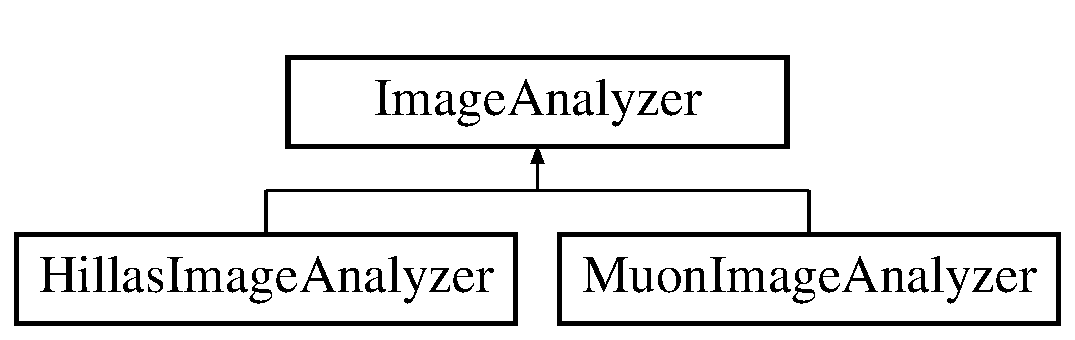
\includegraphics[height=2.000000cm]{classImageAnalyzer}
\end{center}
\end{figure}
\subsubsection*{Public Member Functions}
\begin{DoxyCompactItemize}
\item 
\hypertarget{classImageAnalyzer_a36d9220eab04d031c21237abec9caffd}{
\hyperlink{classImageAnalyzer_a36d9220eab04d031c21237abec9caffd}{ImageAnalyzer} (\hyperlink{classCamera}{Camera} $\ast$cam)}
\label{classImageAnalyzer_a36d9220eab04d031c21237abec9caffd}

\item 
\hypertarget{classImageAnalyzer_aedee9bca28bf1104e6acf113033c4360}{
int {\bfseries getNumPixels} ()}
\label{classImageAnalyzer_aedee9bca28bf1104e6acf113033c4360}

\item 
\hypertarget{classImageAnalyzer_a34ca66f8166b4804c2a03fa0c155f2cc}{
virtual void {\bfseries parameterize} (const Array\_\-t \&image, std::vector$<$ int $>$ \&cleanpixels)=0}
\label{classImageAnalyzer_a34ca66f8166b4804c2a03fa0c155f2cc}

\end{DoxyCompactItemize}
\subsubsection*{Protected Attributes}
\begin{DoxyCompactItemize}
\item 
\hypertarget{classImageAnalyzer_a628d836cd9b04dfb4c14b230498274c0}{
Array\_\-t {\bfseries \_\-x}}
\label{classImageAnalyzer_a628d836cd9b04dfb4c14b230498274c0}

\item 
\hypertarget{classImageAnalyzer_a874a4fdc2fb1c726759f284dcdd66523}{
Array\_\-t {\bfseries \_\-y}}
\label{classImageAnalyzer_a874a4fdc2fb1c726759f284dcdd66523}

\item 
\hypertarget{classImageAnalyzer_ad42c24651b1898531e1c07e734c04aef}{
Array\_\-t {\bfseries \_\-x2}}
\label{classImageAnalyzer_ad42c24651b1898531e1c07e734c04aef}

\item 
\hypertarget{classImageAnalyzer_a544ebef59a5ee33364e44ffa35ab8f7d}{
Array\_\-t {\bfseries \_\-y2}}
\label{classImageAnalyzer_a544ebef59a5ee33364e44ffa35ab8f7d}

\item 
\hypertarget{classImageAnalyzer_acb41487bfeedcdb54f77592f96bbad2c}{
Array\_\-t {\bfseries \_\-xy}}
\label{classImageAnalyzer_acb41487bfeedcdb54f77592f96bbad2c}

\end{DoxyCompactItemize}


\subsubsection{Detailed Description}
Base class for ImageAnalyzers -\/ components that look at an individual image and derive a set of parameters. 

Definition at line 77 of file ImageAnalyzer.h.



The documentation for this class was generated from the following files:\begin{DoxyCompactItemize}
\item 
ImageAnalyzer.h\item 
ImageAnalyzer.cpp\end{DoxyCompactItemize}

\hypertarget{classImageCleaner}{
\subsection{ImageCleaner Class Reference}
\label{classImageCleaner}\index{ImageCleaner@{ImageCleaner}}
}


Abstract interface to all cleaning routines.  




{\ttfamily \#include $<$ImageCleaner.h$>$}

Inheritance diagram for ImageCleaner:\begin{figure}[H]
\begin{center}
\leavevmode
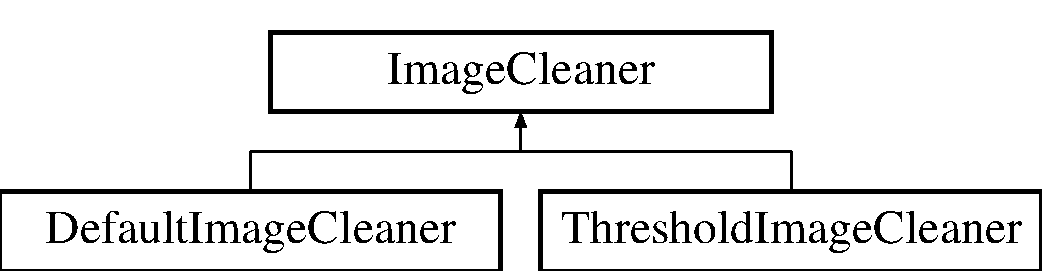
\includegraphics[height=2.000000cm]{classImageCleaner}
\end{center}
\end{figure}
\subsubsection*{Public Member Functions}
\begin{DoxyCompactItemize}
\item 
\hypertarget{classImageCleaner_a027c43146b1e5ab91b8f982b3963b3c9}{
{\bfseries ImageCleaner} (\hyperlink{classCamera}{Camera} \&camera)}
\label{classImageCleaner_a027c43146b1e5ab91b8f982b3963b3c9}

\item 
\hypertarget{classImageCleaner_a05208229b8c2d7bfb618b809d31f849f}{
virtual std::vector$<$ int $>$ \& {\bfseries getCleanPixels} (const Array\_\-t \&image)=0}
\label{classImageCleaner_a05208229b8c2d7bfb618b809d31f849f}

\end{DoxyCompactItemize}
\subsubsection*{Protected Attributes}
\begin{DoxyCompactItemize}
\item 
\hypertarget{classImageCleaner_ad5416a673ec07df1ef62baaf5370f844}{
\hyperlink{classCamera}{Camera} $\ast$ {\bfseries \_\-cam}}
\label{classImageCleaner_ad5416a673ec07df1ef62baaf5370f844}

\end{DoxyCompactItemize}


\subsubsection{Detailed Description}
Abstract interface to all cleaning routines. 

Takes an image as input and spits out a list of pixels which pass the cleaning process. This class can be extended to do more interesting things (such as island cleaning, etc). 

Definition at line 16 of file ImageCleaner.h.



The documentation for this class was generated from the following file:\begin{DoxyCompactItemize}
\item 
ImageCleaner.h\end{DoxyCompactItemize}

\hypertarget{structImageParameterization}{
\subsection{ImageParameterization Struct Reference}
\label{structImageParameterization}\index{ImageParameterization@{ImageParameterization}}
}


Information common to all parameterizations.  




{\ttfamily \#include $<$ImageAnalyzer.h$>$}

Inheritance diagram for ImageParameterization:\begin{figure}[H]
\begin{center}
\leavevmode
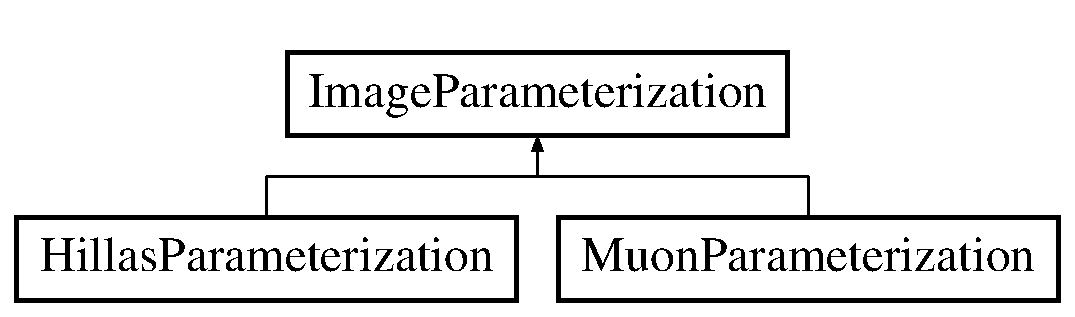
\includegraphics[height=2.000000cm]{structImageParameterization}
\end{center}
\end{figure}
\subsubsection*{Public Attributes}
\begin{DoxyCompactItemize}
\item 
\hypertarget{structImageParameterization_a7190a3fc893a52c1f544d34b09c0368f}{
short \hyperlink{structImageParameterization_a7190a3fc893a52c1f544d34b09c0368f}{telescope\_\-id}}
\label{structImageParameterization_a7190a3fc893a52c1f544d34b09c0368f}

\item 
\hypertarget{structImageParameterization_a3d8a18d1b4e1bf7d7f5b177665651cf4}{
double \hyperlink{structImageParameterization_a3d8a18d1b4e1bf7d7f5b177665651cf4}{osctime}}
\label{structImageParameterization_a3d8a18d1b4e1bf7d7f5b177665651cf4}

\item 
\hypertarget{structImageParameterization_a169f947f6ed26a3097243c8c42c41a64}{
double \hyperlink{structImageParameterization_a169f947f6ed26a3097243c8c42c41a64}{gpstime}}
\label{structImageParameterization_a169f947f6ed26a3097243c8c42c41a64}

\item 
\hypertarget{structImageParameterization_a485ec7c0550f9214971331a7cc2b0b6c}{
double \hyperlink{structImageParameterization_a485ec7c0550f9214971331a7cc2b0b6c}{livetime}}
\label{structImageParameterization_a485ec7c0550f9214971331a7cc2b0b6c}

\item 
\hypertarget{structImageParameterization_a413610cc7481fd731c8b6a0e30d741a0}{
short \hyperlink{structImageParameterization_a413610cc7481fd731c8b6a0e30d741a0}{invalid}}
\label{structImageParameterization_a413610cc7481fd731c8b6a0e30d741a0}

\item 
\hypertarget{structImageParameterization_a3524379a51b511ce132fb97d66e6028b}{
int \hyperlink{structImageParameterization_a3524379a51b511ce132fb97d66e6028b}{event\_\-number}}
\label{structImageParameterization_a3524379a51b511ce132fb97d66e6028b}

\item 
\hypertarget{structImageParameterization_a87de679fb2937a5f1efe38b2c68dea44}{
\hyperlink{structSimShowerRecord}{SimShowerRecord} \hyperlink{structImageParameterization_a87de679fb2937a5f1efe38b2c68dea44}{sim}}
\label{structImageParameterization_a87de679fb2937a5f1efe38b2c68dea44}

\end{DoxyCompactItemize}


\subsubsection{Detailed Description}
Information common to all parameterizations. 

Definition at line 19 of file ImageAnalyzer.h.



The documentation for this struct was generated from the following file:\begin{DoxyCompactItemize}
\item 
ImageAnalyzer.h\end{DoxyCompactItemize}

\hypertarget{classLogger}{
\subsection{Logger Class Reference}
\label{classLogger}\index{Logger@{Logger}}
}


Error log singleton.  




{\ttfamily \#include $<$Log.h$>$}

\subsubsection*{Public Member Functions}
\begin{DoxyCompactItemize}
\item 
\hypertarget{classLogger_a97d14a6dbc7c4490cbe590a0925bc42d}{
void \hyperlink{classLogger_a97d14a6dbc7c4490cbe590a0925bc42d}{printf} (char $\ast$format,...)}
\label{classLogger_a97d14a6dbc7c4490cbe590a0925bc42d}

\item 
\hypertarget{classLogger_ad0747538d6c19da8a5ae15ad6483a997}{
void \hyperlink{classLogger_ad0747538d6c19da8a5ae15ad6483a997}{info} (char $\ast$format,...)}
\label{classLogger_ad0747538d6c19da8a5ae15ad6483a997}

\item 
\hypertarget{classLogger_a4739f36877383f53e3ce13200087a104}{
int {\bfseries getErrorCount} ()}
\label{classLogger_a4739f36877383f53e3ce13200087a104}

\item 
\hypertarget{classLogger_a01d17329a2a7f038570c6c769c90cdef}{
void {\bfseries printLog} ()}
\label{classLogger_a01d17329a2a7f038570c6c769c90cdef}

\item 
\hypertarget{classLogger_a5e7512550a4c84d23de47454356aa8f2}{
std::string {\bfseries getFileName} ()}
\label{classLogger_a5e7512550a4c84d23de47454356aa8f2}

\end{DoxyCompactItemize}
\subsubsection*{Static Public Member Functions}
\begin{DoxyCompactItemize}
\item 
\hypertarget{classLogger_a9f9acae64a5f26267526d16196ea23c8}{
static \hyperlink{classLogger}{Logger} $\ast$ {\bfseries instance} ()}
\label{classLogger_a9f9acae64a5f26267526d16196ea23c8}

\end{DoxyCompactItemize}


\subsubsection{Detailed Description}
Error log singleton. 

Calling the \hyperlink{classLogger_a97d14a6dbc7c4490cbe590a0925bc42d}{printf()} function will write to the log. 

Definition at line 16 of file Log.h.



The documentation for this class was generated from the following files:\begin{DoxyCompactItemize}
\item 
Log.h\item 
Log.cpp\end{DoxyCompactItemize}

\hypertarget{structLZAEnergyEstimator}{
\subsection{LZAEnergyEstimator Struct Reference}
\label{structLZAEnergyEstimator}\index{LZAEnergyEstimator@{LZAEnergyEstimator}}
}
Inheritance diagram for LZAEnergyEstimator:\begin{figure}[H]
\begin{center}
\leavevmode
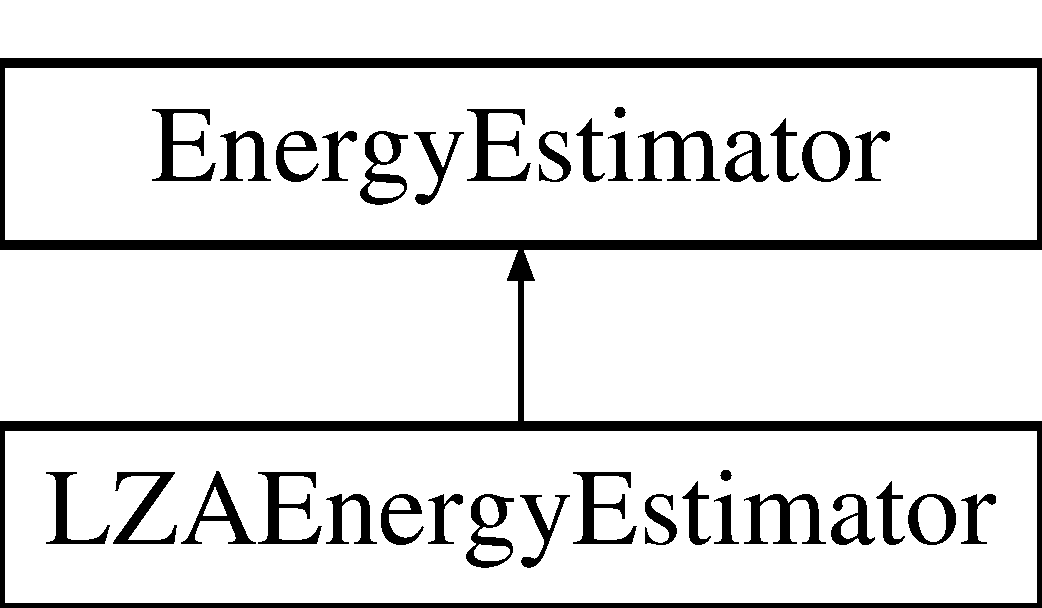
\includegraphics[height=2.000000cm]{structLZAEnergyEstimator}
\end{center}
\end{figure}
\subsubsection*{Public Member Functions}
\begin{DoxyCompactItemize}
\item 
double \hyperlink{structLZAEnergyEstimator_af0411fdc8594f35df402e97ef913b109}{getEstimate} (const double size, const double distance, const double zenith=1.04719755)
\end{DoxyCompactItemize}


\subsubsection{Detailed Description}


Definition at line 44 of file EnergySpectrum.h.



\subsubsection{Member Function Documentation}
\hypertarget{structLZAEnergyEstimator_af0411fdc8594f35df402e97ef913b109}{
\index{LZAEnergyEstimator@{LZAEnergyEstimator}!getEstimate@{getEstimate}}
\index{getEstimate@{getEstimate}!LZAEnergyEstimator@{LZAEnergyEstimator}}
\paragraph[{getEstimate}]{\setlength{\rightskip}{0pt plus 5cm}double LZAEnergyEstimator::getEstimate (
\begin{DoxyParamCaption}
\item[{const double}]{size, }
\item[{const double}]{dist, }
\item[{const double}]{zenith = {\ttfamily 1.04719755}}
\end{DoxyParamCaption}
)\hspace{0.3cm}{\ttfamily  \mbox{[}virtual\mbox{]}}}}
\label{structLZAEnergyEstimator_af0411fdc8594f35df402e97ef913b109}


Energy estimator for LZA (Z $\sim$= 30 degrees) data. 

This function, which was fit to simulation data, returns the log10 of the estimated energy (log10(EstimatedEnergy)) 

Implements \hyperlink{structEnergyEstimator}{EnergyEstimator}.



Definition at line 18 of file EnergySpectrum.cpp.



The documentation for this struct was generated from the following files:\begin{DoxyCompactItemize}
\item 
EnergySpectrum.h\item 
EnergySpectrum.cpp\end{DoxyCompactItemize}

\hypertarget{structMCBinInfo}{
\subsection{MCBinInfo Struct Reference}
\label{structMCBinInfo}\index{MCBinInfo@{MCBinInfo}}
}
\subsubsection*{Public Attributes}
\begin{DoxyCompactItemize}
\item 
\hypertarget{structMCBinInfo_a977c6f52ec69f4842527706115ce91bf}{
double {\bfseries start}}
\label{structMCBinInfo_a977c6f52ec69f4842527706115ce91bf}

\item 
\hypertarget{structMCBinInfo_a964eaa282a44156c957e26eea27c8374}{
double {\bfseries end}}
\label{structMCBinInfo_a964eaa282a44156c957e26eea27c8374}

\item 
\hypertarget{structMCBinInfo_aaea60de9155baf52311a4664d5bd530b}{
double {\bfseries radius}}
\label{structMCBinInfo_aaea60de9155baf52311a4664d5bd530b}

\item 
\hypertarget{structMCBinInfo_a541d4c5a4903e5246343e07ac4bcb04c}{
int {\bfseries nummc}}
\label{structMCBinInfo_a541d4c5a4903e5246343e07ac4bcb04c}

\end{DoxyCompactItemize}


\subsubsection{Detailed Description}


Definition at line 75 of file Fitter.h.



The documentation for this struct was generated from the following files:\begin{DoxyCompactItemize}
\item 
Fitter.h\item 
FitterNew.h\end{DoxyCompactItemize}

\hypertarget{structMCRecord}{
\subsection{MCRecord Struct Reference}
\label{structMCRecord}\index{MCRecord@{MCRecord}}
}


For Each Monte Carlo Event That Passes the Selection \hyperlink{namespaceCuts}{Cuts}, We Want to Know the True Energy and the Reconstructed Energy.  




{\ttfamily \#include $<$Fitter.h$>$}

\subsubsection*{Public Attributes}
\begin{DoxyCompactItemize}
\item 
\hypertarget{structMCRecord_a47c1e228820b8bf3de8c9d959963a504}{
double {\bfseries trueEnergy\_\-in\_\-TeV}}
\label{structMCRecord_a47c1e228820b8bf3de8c9d959963a504}

\item 
\hypertarget{structMCRecord_aef6015e2be171bc4fc42be18a4108ad0}{
double {\bfseries estimatedEnergy}}
\label{structMCRecord_aef6015e2be171bc4fc42be18a4108ad0}

\end{DoxyCompactItemize}


\subsubsection{Detailed Description}
For Each Monte Carlo Event That Passes the Selection \hyperlink{namespaceCuts}{Cuts}, We Want to Know the True Energy and the Reconstructed Energy. 

Definition at line 50 of file Fitter.h.



The documentation for this struct was generated from the following files:\begin{DoxyCompactItemize}
\item 
Fitter.h\item 
FitterNew.h\end{DoxyCompactItemize}

\hypertarget{classMCSpectrum}{
\subsection{MCSpectrum Class Reference}
\label{classMCSpectrum}\index{MCSpectrum@{MCSpectrum}}
}


Object that takes care of all the Monte Carlo (MC) dependent aspects:  




{\ttfamily \#include $<$Fitter.h$>$}

\subsubsection*{Public Member Functions}
\begin{DoxyCompactItemize}
\item 
\hyperlink{classMCSpectrum_ae7bb310b53fe6faf2fbdb74017c627db}{MCSpectrum} (\hyperlink{classRunInfo}{RunInfo} \&ri)
\item 
\hypertarget{classMCSpectrum_a7e79cfbd1d264d02e46010375e399aca}{
void \hyperlink{classMCSpectrum_a7e79cfbd1d264d02e46010375e399aca}{fill} (double N0, double Gamma0, double E0, double Time)}
\label{classMCSpectrum_a7e79cfbd1d264d02e46010375e399aca}

\item 
\hypertarget{classMCSpectrum_a0777ca61a540ea776229d523ff32b0f4}{
double \hyperlink{classMCSpectrum_a0777ca61a540ea776229d523ff32b0f4}{chiSquare} (std::vector$<$ \hyperlink{structData}{Data} $>$ \&)}
\label{classMCSpectrum_a0777ca61a540ea776229d523ff32b0f4}

\item 
\hypertarget{classMCSpectrum_ad677cf1fbb8de27981202ad6056ebf58}{
int \hyperlink{classMCSpectrum_ad677cf1fbb8de27981202ad6056ebf58}{dof} ()}
\label{classMCSpectrum_ad677cf1fbb8de27981202ad6056ebf58}

\item 
\hypertarget{classMCSpectrum_aadcdac2c8cf36b4c6b76f9c0f7a04d65}{
double \hyperlink{classMCSpectrum_aadcdac2c8cf36b4c6b76f9c0f7a04d65}{get} (int)}
\label{classMCSpectrum_aadcdac2c8cf36b4c6b76f9c0f7a04d65}

\item 
\hypertarget{classMCSpectrum_aea3d956882a19612b53dfabf4a4ee36f}{
void \hyperlink{classMCSpectrum_aea3d956882a19612b53dfabf4a4ee36f}{getRange} (int bin, double \&lower, double \&upper)}
\label{classMCSpectrum_aea3d956882a19612b53dfabf4a4ee36f}

\item 
\hypertarget{classMCSpectrum_aff6aa85d0e2a5006caf0b194ec53dae1}{
\hyperlink{classEnergySpectrum}{EnergySpectrum} $\ast$ {\bfseries getSpectrum} ()}
\label{classMCSpectrum_aff6aa85d0e2a5006caf0b194ec53dae1}

\item 
\hypertarget{classMCSpectrum_ae7bb310b53fe6faf2fbdb74017c627db}{
{\bfseries MCSpectrum} (\hyperlink{classRunInfo}{RunInfo} \&ri)}
\label{classMCSpectrum_ae7bb310b53fe6faf2fbdb74017c627db}

\item 
\hypertarget{classMCSpectrum_a7e79cfbd1d264d02e46010375e399aca}{
void {\bfseries fill} (double N0, double Gamma0, double E0, double Time)}
\label{classMCSpectrum_a7e79cfbd1d264d02e46010375e399aca}

\item 
\hypertarget{classMCSpectrum_a0777ca61a540ea776229d523ff32b0f4}{
double {\bfseries chiSquare} (std::vector$<$ \hyperlink{structData}{Data} $>$ \&)}
\label{classMCSpectrum_a0777ca61a540ea776229d523ff32b0f4}

\item 
\hypertarget{classMCSpectrum_ad677cf1fbb8de27981202ad6056ebf58}{
int {\bfseries dof} ()}
\label{classMCSpectrum_ad677cf1fbb8de27981202ad6056ebf58}

\item 
\hypertarget{classMCSpectrum_aadcdac2c8cf36b4c6b76f9c0f7a04d65}{
double {\bfseries get} (int)}
\label{classMCSpectrum_aadcdac2c8cf36b4c6b76f9c0f7a04d65}

\item 
\hypertarget{classMCSpectrum_aea3d956882a19612b53dfabf4a4ee36f}{
void {\bfseries getRange} (int bin, double \&lower, double \&upper)}
\label{classMCSpectrum_aea3d956882a19612b53dfabf4a4ee36f}

\item 
\hypertarget{classMCSpectrum_aff6aa85d0e2a5006caf0b194ec53dae1}{
\hyperlink{classEnergySpectrum}{EnergySpectrum} $\ast$ {\bfseries getSpectrum} ()}
\label{classMCSpectrum_aff6aa85d0e2a5006caf0b194ec53dae1}

\end{DoxyCompactItemize}
\subsubsection*{Static Public Attributes}
\begin{DoxyCompactItemize}
\item 
\hypertarget{classMCSpectrum_a331195d13e485713885e0a195654e44c}{
static const int {\bfseries NUMMCBINS} = 9}
\label{classMCSpectrum_a331195d13e485713885e0a195654e44c}

\end{DoxyCompactItemize}


\subsubsection{Detailed Description}
Object that takes care of all the Monte Carlo (MC) dependent aspects: 


\begin{DoxyItemize}
\item it stores the MC events
\end{DoxyItemize}


\begin{DoxyItemize}
\item given model parameters, it can produce histograms with \char`\"{}artficial\char`\"{} energy spectra that can be compared to the data
\end{DoxyItemize}


\begin{DoxyItemize}
\item given a pointer to the data, and a filled \char`\"{}artificial\char`\"{} energy spectrum, it will compute the chi-\/square value. 
\end{DoxyItemize}

Definition at line 96 of file Fitter.h.



\subsubsection{Constructor \& Destructor Documentation}
\hypertarget{classMCSpectrum_ae7bb310b53fe6faf2fbdb74017c627db}{
\index{MCSpectrum@{MCSpectrum}!MCSpectrum@{MCSpectrum}}
\index{MCSpectrum@{MCSpectrum}!MCSpectrum@{MCSpectrum}}
\paragraph[{MCSpectrum}]{\setlength{\rightskip}{0pt plus 5cm}MCSpectrum::MCSpectrum (
\begin{DoxyParamCaption}
\item[{{\bf RunInfo} \&}]{ri}
\end{DoxyParamCaption}
)}}
\label{classMCSpectrum_ae7bb310b53fe6faf2fbdb74017c627db}


Creator, gets all the MC information. 

\begin{Desc}
\item[\hyperlink{todo__todo000013}{Todo}]: make the specific energy estimator function user selectable (LZA vs small zenith, etc.) \end{Desc}


\begin{Desc}
\item[\hyperlink{todo__todo000017}{Todo}]: make the specific energy estimator function user selectable (LZA vs small zenith, etc.) \end{Desc}


Definition at line 45 of file Fitter.cpp.



References RunInfo::cuts, HillasParameterization::distance, RunInfo::energyestimator, EnergyEstimatorFactory::instance(), RunInfo::mcdatabase, ProgressBar::print(), ProgressBar::printClear(), ImageParameterization::sim, HillasParameterization::size, and HillasParameterization::zenith.



The documentation for this class was generated from the following files:\begin{DoxyCompactItemize}
\item 
Fitter.h\item 
FitterNew.h\item 
Fitter.cpp\item 
FitterNew.cpp\end{DoxyCompactItemize}

\hypertarget{classMildAnalysisException}{
\subsection{MildAnalysisException Class Reference}
\label{classMildAnalysisException}\index{MildAnalysisException@{MildAnalysisException}}
}


Thrown for warnings and recoverable errors.  




{\ttfamily \#include $<$Exceptions.h$>$}

Inheritance diagram for MildAnalysisException:\begin{figure}[H]
\begin{center}
\leavevmode
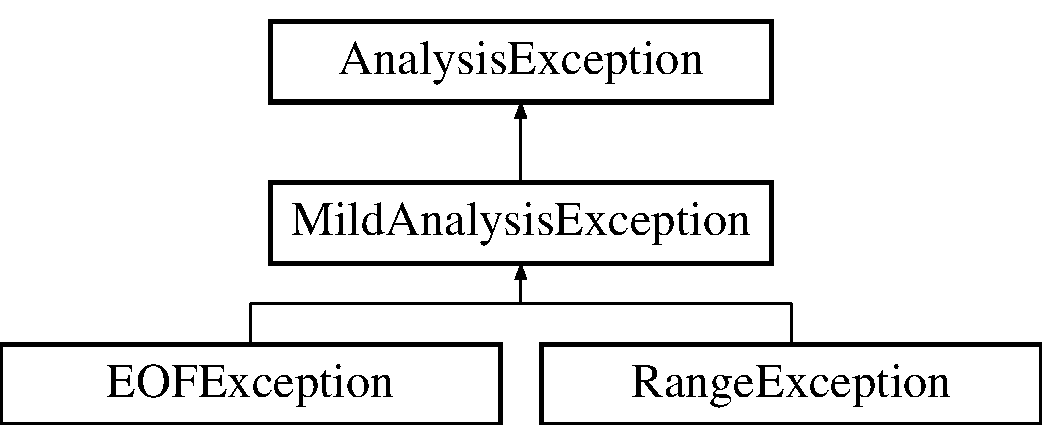
\includegraphics[height=3.000000cm]{classMildAnalysisException}
\end{center}
\end{figure}
\subsubsection*{Public Member Functions}
\begin{DoxyCompactItemize}
\item 
\hypertarget{classMildAnalysisException_a3e7d6c6178a00933856fac70f136c145}{
{\bfseries MildAnalysisException} (const std::string \&str)}
\label{classMildAnalysisException_a3e7d6c6178a00933856fac70f136c145}

\end{DoxyCompactItemize}


\subsubsection{Detailed Description}
Thrown for warnings and recoverable errors. 

Definition at line 41 of file Exceptions.h.



The documentation for this class was generated from the following file:\begin{DoxyCompactItemize}
\item 
Exceptions.h\end{DoxyCompactItemize}

\hypertarget{classMuonImageAnalyzer}{
\subsection{MuonImageAnalyzer Class Reference}
\label{classMuonImageAnalyzer}\index{MuonImageAnalyzer@{MuonImageAnalyzer}}
}


Analyzes the muon-\/like properties of an image.  




{\ttfamily \#include $<$MuonImageAnalyzer.h$>$}

Inheritance diagram for MuonImageAnalyzer:\begin{figure}[H]
\begin{center}
\leavevmode
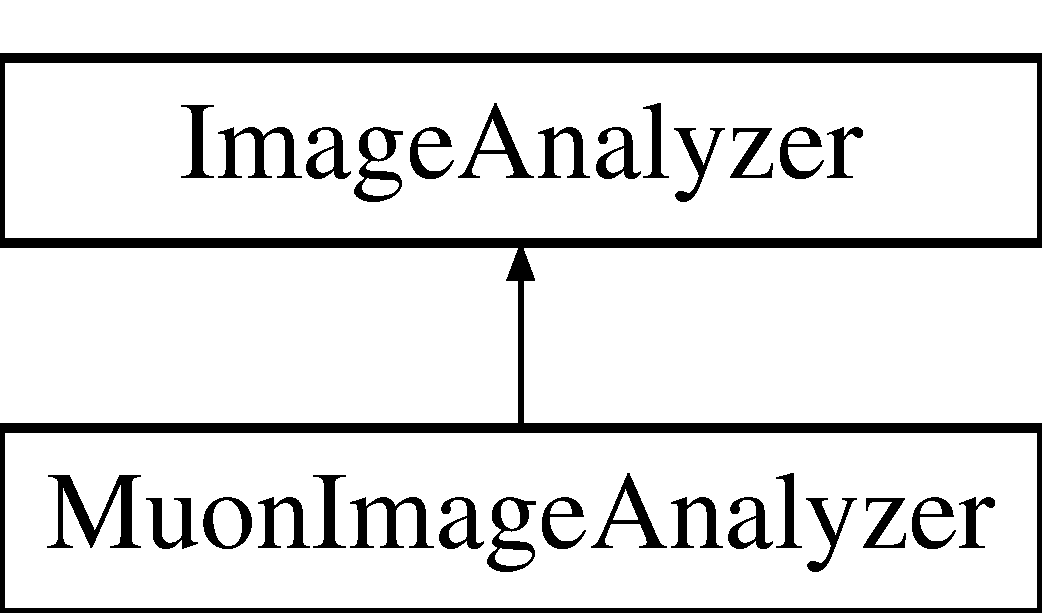
\includegraphics[height=2.000000cm]{classMuonImageAnalyzer}
\end{center}
\end{figure}
\subsubsection*{Classes}
\begin{DoxyCompactItemize}
\item 
struct {\bfseries Triplet}
\item 
struct {\bfseries WordBitMask}
\end{DoxyCompactItemize}
\subsubsection*{Public Member Functions}
\begin{DoxyCompactItemize}
\item 
\hypertarget{classMuonImageAnalyzer_ace536b6518d8bfcbc14afbd252c2cedb}{
\hyperlink{classMuonImageAnalyzer_ace536b6518d8bfcbc14afbd252c2cedb}{MuonImageAnalyzer} (\hyperlink{classCamera}{Camera} $\ast$cam)}
\label{classMuonImageAnalyzer_ace536b6518d8bfcbc14afbd252c2cedb}

\item 
void \hyperlink{classMuonImageAnalyzer_a539a77fa50b32358483b951ceaca22bf}{parameterize} (const Array\_\-t \&image, std::vector$<$ int $>$ \&cleanpixels)
\item 
\hypertarget{classMuonImageAnalyzer_ac13b60121bd5008c0188dfd7d3a04112}{
void {\bfseries enablePlotPoints} (bool val=true)}
\label{classMuonImageAnalyzer_ac13b60121bd5008c0188dfd7d3a04112}

\item 
\hypertarget{classMuonImageAnalyzer_af5825426d2866ab9613d13621bee5867}{
void {\bfseries enableCalibration} (bool val=true)}
\label{classMuonImageAnalyzer_af5825426d2866ab9613d13621bee5867}

\item 
\hyperlink{structMuonParameterization}{MuonParameterization} \hyperlink{classMuonImageAnalyzer_a2b82168624627844ea7502fb3a182767}{getMuonParameters} ()
\end{DoxyCompactItemize}


\subsubsection{Detailed Description}
Analyzes the muon-\/like properties of an image. 

In particular, it detects muon arcs and can calculates factors useful for absolute gain calibration.

The algorithm goes as follows:


\begin{DoxyItemize}
\item For each unique triplet of PMTs (N$\ast$(N-\/1)$\ast$(N-\/2)/6 in total) calculate the center and radius of the uniquely defined circle.
\end{DoxyItemize}


\begin{DoxyItemize}
\item OR the bits for PMTs which are elements of this triplet into the appropriate element (determined by the ring center) of a 2-\/d array of bitmasks, and increment the corresponding element of the array ntriplets\mbox{[}x,y\mbox{]}. Also increment the cumulative ring radius and cumulative x and y-\/center position arrays rad\mbox{[}x,y\mbox{]} xsum\mbox{[}x,y\mbox{]}, ysum\mbox{[}x,y\mbox{]}.
\end{DoxyItemize}


\begin{DoxyItemize}
\item Divide xsum, ysum, radsum by ntriplets in the end. Then do a boxcar average over neighboring elements in the array ntriplets, and x,y,rad arrays.
\end{DoxyItemize}


\begin{DoxyItemize}
\item Find the maximum of the boxcar averaged array ntripbox(x,y) and calculate the values xave,yave,rave from these.
\end{DoxyItemize}


\begin{DoxyItemize}
\item Calculate a bitmask (for which tubes are in the arc) by ORing together the bitmasks of the peak element and its neighbors. From the resulting bitmask calculate the signal sum for these pmts and divide by the number of pmts.
\end{DoxyItemize}

This gives a value proportional to the pe/dc ratio for this arc. A comparison of this value to the value derived for big rings (from the hadronicity) can be combined with limits on the ring radius to derive the likelihood that this event is in fact a muon arc. 

Definition at line 120 of file MuonImageAnalyzer.h.



\subsubsection{Member Function Documentation}
\hypertarget{classMuonImageAnalyzer_a2b82168624627844ea7502fb3a182767}{
\index{MuonImageAnalyzer@{MuonImageAnalyzer}!getMuonParameters@{getMuonParameters}}
\index{getMuonParameters@{getMuonParameters}!MuonImageAnalyzer@{MuonImageAnalyzer}}
\paragraph[{getMuonParameters}]{\setlength{\rightskip}{0pt plus 5cm}{\bf MuonParameterization} MuonImageAnalyzer::getMuonParameters (
\begin{DoxyParamCaption}
{}
\end{DoxyParamCaption}
)\hspace{0.3cm}{\ttfamily  \mbox{[}inline\mbox{]}}}}
\label{classMuonImageAnalyzer_a2b82168624627844ea7502fb3a182767}


Get the parameters calculated in the \hyperlink{classMuonImageAnalyzer_a539a77fa50b32358483b951ceaca22bf}{parameterize()} routine. 

\begin{DoxyReturn}{Returns}
a \hyperlink{structMuonParameterization}{MuonParameterization} containing all the parameters 
\end{DoxyReturn}


Definition at line 135 of file MuonImageAnalyzer.h.

\hypertarget{classMuonImageAnalyzer_a539a77fa50b32358483b951ceaca22bf}{
\index{MuonImageAnalyzer@{MuonImageAnalyzer}!parameterize@{parameterize}}
\index{parameterize@{parameterize}!MuonImageAnalyzer@{MuonImageAnalyzer}}
\paragraph[{parameterize}]{\setlength{\rightskip}{0pt plus 5cm}void MuonImageAnalyzer::parameterize (
\begin{DoxyParamCaption}
\item[{const Array\_\-t \&}]{image, }
\item[{std::vector$<$ int $>$ \&}]{cleanpixels}
\end{DoxyParamCaption}
)\hspace{0.3cm}{\ttfamily  \mbox{[}virtual\mbox{]}}}}
\label{classMuonImageAnalyzer_a539a77fa50b32358483b951ceaca22bf}


Parameterize the image. 

Find muon arc and calculate parameters.

This is the most important (and probably the most called) function in the analysis, so it should be as optimized as possible!


\begin{DoxyParams}{Parameters}
{\em image} & the pixel data for the image you want to parameterize \\
\hline
{\em cleanpixels} & is a list of the indices of the picture/boundary tubes parameters should be stored.\\
\hline
{\em image} & the image \\
\hline
{\em cleanpixels} & vector of clean pixel numbers from \\
\hline
\end{DoxyParams}


Implements \hyperlink{classImageAnalyzer}{ImageAnalyzer}.



Definition at line 84 of file ImageAnalyzer.cpp.



References HillasParameterization::alpha, HillasParameterization::asymmetry, HillasParameterization::azwidth, HillasParameterization::centroid, HillasParameterization::distance, HillasParameterization::frac, HillasParameterization::index\_\-of\_\-max, ImageParameterization::invalid, HillasParameterization::length, HillasParameterization::length\_\-over\_\-size, HillasParameterization::max, HillasParameterization::miss, HillasParameterization::phi, HillasParameterization::pixels\_\-in\_\-picture, HillasParameterization::point\_\-of\_\-origin\_\-a, HillasParameterization::point\_\-of\_\-origin\_\-b, HillasParameterization::psi, HillasParameterization::size, HillasParameterization::width, Coordinate\_\-t::x, and Coordinate\_\-t::y.



The documentation for this class was generated from the following files:\begin{DoxyCompactItemize}
\item 
MuonImageAnalyzer.h\item 
ImageAnalyzer.cpp\item 
MuonImageAnalyzer.cpp\end{DoxyCompactItemize}

\hypertarget{structMuonParameterization}{
\subsection{MuonParameterization Struct Reference}
\label{structMuonParameterization}\index{MuonParameterization@{MuonParameterization}}
}


Describes the muon-\/like characteristics of an image.  




{\ttfamily \#include $<$MuonImageAnalyzer.h$>$}

Inheritance diagram for MuonParameterization:\begin{figure}[H]
\begin{center}
\leavevmode
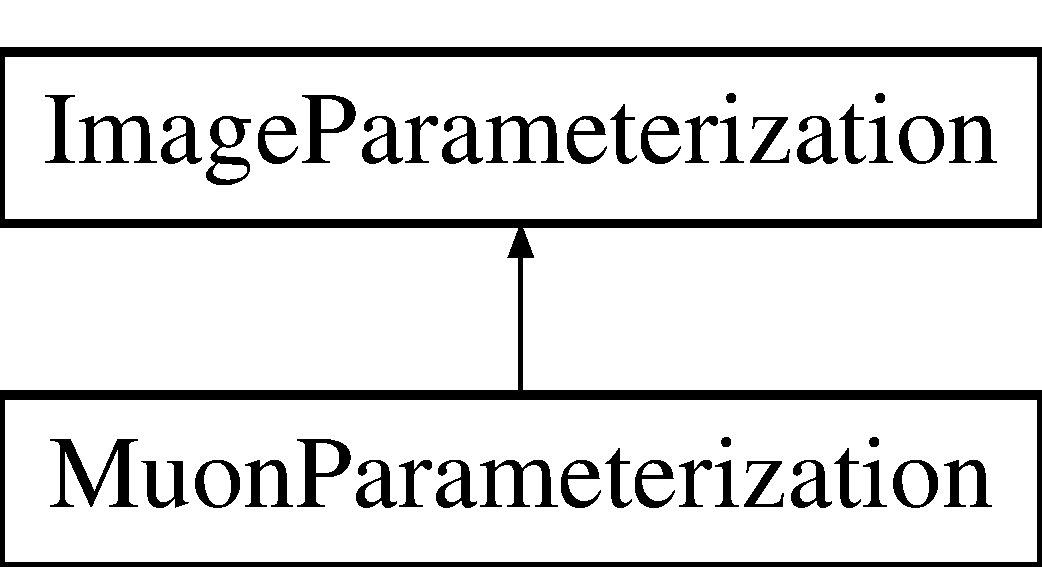
\includegraphics[height=2.000000cm]{structMuonParameterization}
\end{center}
\end{figure}
\subsubsection*{Public Member Functions}
\begin{DoxyCompactItemize}
\item 
\hypertarget{structMuonParameterization_a3f667029da45f04fb632f74538db3fa9}{
void {\bfseries clear} ()}
\label{structMuonParameterization_a3f667029da45f04fb632f74538db3fa9}

\end{DoxyCompactItemize}
\subsubsection*{Public Attributes}
\begin{DoxyCompactItemize}
\item 
\hypertarget{structMuonParameterization_a9288b7b7437754b412d98df17ea096f3}{
double \hyperlink{structMuonParameterization_a9288b7b7437754b412d98df17ea096f3}{radius}}
\label{structMuonParameterization_a9288b7b7437754b412d98df17ea096f3}

\item 
\hypertarget{structMuonParameterization_a777390dd328e115a3acfdccde4cec092}{
\hyperlink{structCoordinate__t}{Coordinate\_\-t} \hyperlink{structMuonParameterization_a777390dd328e115a3acfdccde4cec092}{ringcenter}}
\label{structMuonParameterization_a777390dd328e115a3acfdccde4cec092}

\item 
\hypertarget{structMuonParameterization_a44a8fe62958828b38511317f19aeeb8c}{
double \hyperlink{structMuonParameterization_a44a8fe62958828b38511317f19aeeb8c}{arcstrength}}
\label{structMuonParameterization_a44a8fe62958828b38511317f19aeeb8c}

\item 
\hypertarget{structMuonParameterization_af18698c7eb37805625db4d32be9622e7}{
double \hyperlink{structMuonParameterization_af18698c7eb37805625db4d32be9622e7}{gain}}
\label{structMuonParameterization_af18698c7eb37805625db4d32be9622e7}

\item 
\hypertarget{structMuonParameterization_aca865edfe191cfad91502c0cc71d9eb8}{
double \hyperlink{structMuonParameterization_aca865edfe191cfad91502c0cc71d9eb8}{mugain}}
\label{structMuonParameterization_aca865edfe191cfad91502c0cc71d9eb8}

\item 
\hypertarget{structMuonParameterization_a23be272cf46718ffa72f9714986f37ae}{
double \hyperlink{structMuonParameterization_a23be272cf46718ffa72f9714986f37ae}{ringfrac}}
\label{structMuonParameterization_a23be272cf46718ffa72f9714986f37ae}

\item 
\hypertarget{structMuonParameterization_a5755c497600535efe649802773ff2919}{
double \hyperlink{structMuonParameterization_a5755c497600535efe649802773ff2919}{soal}}
\label{structMuonParameterization_a5755c497600535efe649802773ff2919}

\item 
\hypertarget{structMuonParameterization_a0f5e861cb63b098fb9ceb5dcedbc3f1f}{
double \hyperlink{structMuonParameterization_a0f5e861cb63b098fb9ceb5dcedbc3f1f}{muskew}}
\label{structMuonParameterization_a0f5e861cb63b098fb9ceb5dcedbc3f1f}

\item 
\hypertarget{structMuonParameterization_a6d7831ff9cb8f6195ffdd74aefd03c79}{
double \hyperlink{structMuonParameterization_a6d7831ff9cb8f6195ffdd74aefd03c79}{arclen}}
\label{structMuonParameterization_a6d7831ff9cb8f6195ffdd74aefd03c79}

\item 
\hypertarget{structMuonParameterization_a4cb5fe9a4160ed1cc399fa650e04e8b4}{
double \hyperlink{structMuonParameterization_a4cb5fe9a4160ed1cc399fa650e04e8b4}{philo}}
\label{structMuonParameterization_a4cb5fe9a4160ed1cc399fa650e04e8b4}

\item 
\hypertarget{structMuonParameterization_a58ab3dbbf899d2ecb0f5dff749e5e159}{
double \hyperlink{structMuonParameterization_a58ab3dbbf899d2ecb0f5dff749e5e159}{phihi}}
\label{structMuonParameterization_a58ab3dbbf899d2ecb0f5dff749e5e159}

\item 
\hypertarget{structMuonParameterization_a57d9f4eb8eec896b0bfd052900e6b64c}{
double \hyperlink{structMuonParameterization_a57d9f4eb8eec896b0bfd052900e6b64c}{phimid}}
\label{structMuonParameterization_a57d9f4eb8eec896b0bfd052900e6b64c}

\item 
\hypertarget{structMuonParameterization_a90ef1e6a695a8470b7192acd0ea43674}{
\hyperlink{structCoordinate__t}{Coordinate\_\-t} \hyperlink{structMuonParameterization_a90ef1e6a695a8470b7192acd0ea43674}{plot} \mbox{[}MAX\_\-PLOT\_\-CENTERS\mbox{]}}
\label{structMuonParameterization_a90ef1e6a695a8470b7192acd0ea43674}

\item 
\hypertarget{structMuonParameterization_a7101e63412d2ef8fd2ef81891f8433b2}{
int \hyperlink{structMuonParameterization_a7101e63412d2ef8fd2ef81891f8433b2}{nplotpoints}}
\label{structMuonParameterization_a7101e63412d2ef8fd2ef81891f8433b2}

\item 
\hypertarget{structMuonParameterization_a2ebceb539977f87168c1f88efbb2dec6}{
double \hyperlink{structMuonParameterization_a2ebceb539977f87168c1f88efbb2dec6}{muonness}}
\label{structMuonParameterization_a2ebceb539977f87168c1f88efbb2dec6}

\item 
\hypertarget{structMuonParameterization_a3ddd93b4356814777ef6a1896d9f98f4}{
double \hyperlink{structMuonParameterization_a3ddd93b4356814777ef6a1896d9f98f4}{smoothness}}
\label{structMuonParameterization_a3ddd93b4356814777ef6a1896d9f98f4}

\item 
\hypertarget{structMuonParameterization_a8787f6467e1d4ffca5bbc1a96c6f64e7}{
double \hyperlink{structMuonParameterization_a8787f6467e1d4ffca5bbc1a96c6f64e7}{smoothness\_\-var}}
\label{structMuonParameterization_a8787f6467e1d4ffca5bbc1a96c6f64e7}

\item 
\hypertarget{structMuonParameterization_a9415f852432d71ea7c2d639d0336a1fc}{
double {\bfseries xcs}}
\label{structMuonParameterization_a9415f852432d71ea7c2d639d0336a1fc}

\item 
\hypertarget{structMuonParameterization_aab3debf8a20b5743eab93e3cc49b7c37}{
double {\bfseries ycs}}
\label{structMuonParameterization_aab3debf8a20b5743eab93e3cc49b7c37}

\item 
\hypertarget{structMuonParameterization_a07067d0d35d7409a7b46ebd3d95a344d}{
double {\bfseries rspread}}
\label{structMuonParameterization_a07067d0d35d7409a7b46ebd3d95a344d}

\end{DoxyCompactItemize}


\subsubsection{Detailed Description}
Describes the muon-\/like characteristics of an image. 

Definition at line 32 of file MuonImageAnalyzer.h.



The documentation for this struct was generated from the following file:\begin{DoxyCompactItemize}
\item 
MuonImageAnalyzer.h\end{DoxyCompactItemize}

\hypertarget{structOption__s}{
\subsection{Option\_\-s Struct Reference}
\label{structOption__s}\index{Option\_\-s@{Option\_\-s}}
}
\subsubsection*{Public Attributes}
\begin{DoxyCompactItemize}
\item 
\hypertarget{structOption__s_a09d8a06dd676f09df38bcdd27b7d7fbe}{
bool {\bfseries verbose}}
\label{structOption__s_a09d8a06dd676f09df38bcdd27b7d7fbe}

\item 
\hypertarget{structOption__s_a47776a1c608f1bd214d53118a3710453}{
bool {\bfseries interactive}}
\label{structOption__s_a47776a1c608f1bd214d53118a3710453}

\item 
\hypertarget{structOption__s_aa34cf8e9d474d35d4ee08ba63c49d49b}{
bool {\bfseries display}}
\label{structOption__s_aa34cf8e9d474d35d4ee08ba63c49d49b}

\item 
\hypertarget{structOption__s_a66d749f5a5f87341a44fad6bc4c04a44}{
bool {\bfseries overwrite}}
\label{structOption__s_a66d749f5a5f87341a44fad6bc4c04a44}

\item 
\hypertarget{structOption__s_a607ba585080fc346d78962c37b37c2dc}{
bool {\bfseries clearcache}}
\label{structOption__s_a607ba585080fc346d78962c37b37c2dc}

\end{DoxyCompactItemize}


\subsubsection{Detailed Description}


Definition at line 20 of file wuparam.h.



The documentation for this struct was generated from the following file:\begin{DoxyCompactItemize}
\item 
wuparam.h\end{DoxyCompactItemize}

\hypertarget{classPairRunInfo}{
\subsection{PairRunInfo Class Reference}
\label{classPairRunInfo}\index{PairRunInfo@{PairRunInfo}}
}
Inheritance diagram for PairRunInfo:\begin{figure}[H]
\begin{center}
\leavevmode
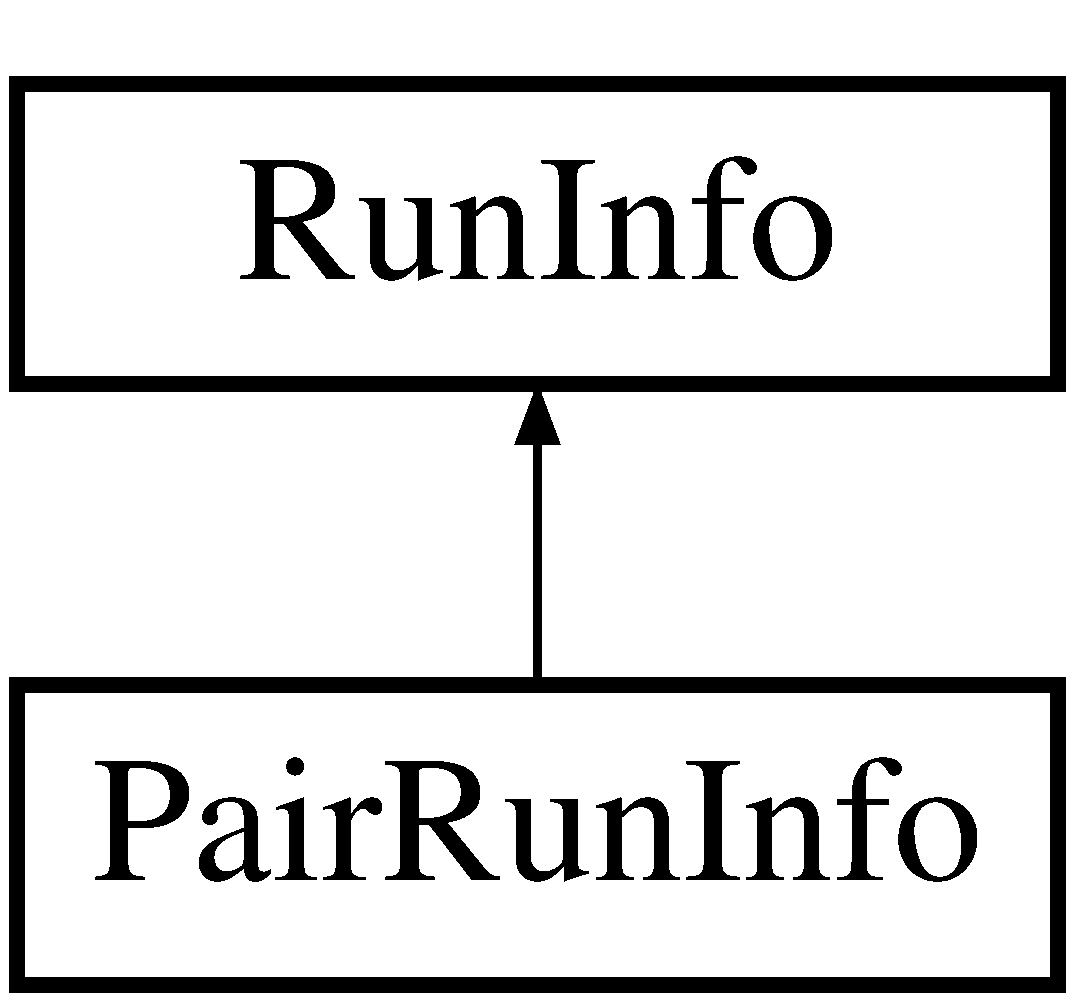
\includegraphics[height=2.000000cm]{classPairRunInfo}
\end{center}
\end{figure}


\subsubsection{Detailed Description}


Definition at line 182 of file Config.h.



The documentation for this class was generated from the following file:\begin{DoxyCompactItemize}
\item 
Config.h\end{DoxyCompactItemize}

\hypertarget{classParamDataReader}{
\subsection{ParamDataReader Class Reference}
\label{classParamDataReader}\index{ParamDataReader@{ParamDataReader}}
}


Reads parameterized datafiles.  




{\ttfamily \#include $<$ParamDataReader.h$>$}

Inheritance diagram for ParamDataReader:\begin{figure}[H]
\begin{center}
\leavevmode
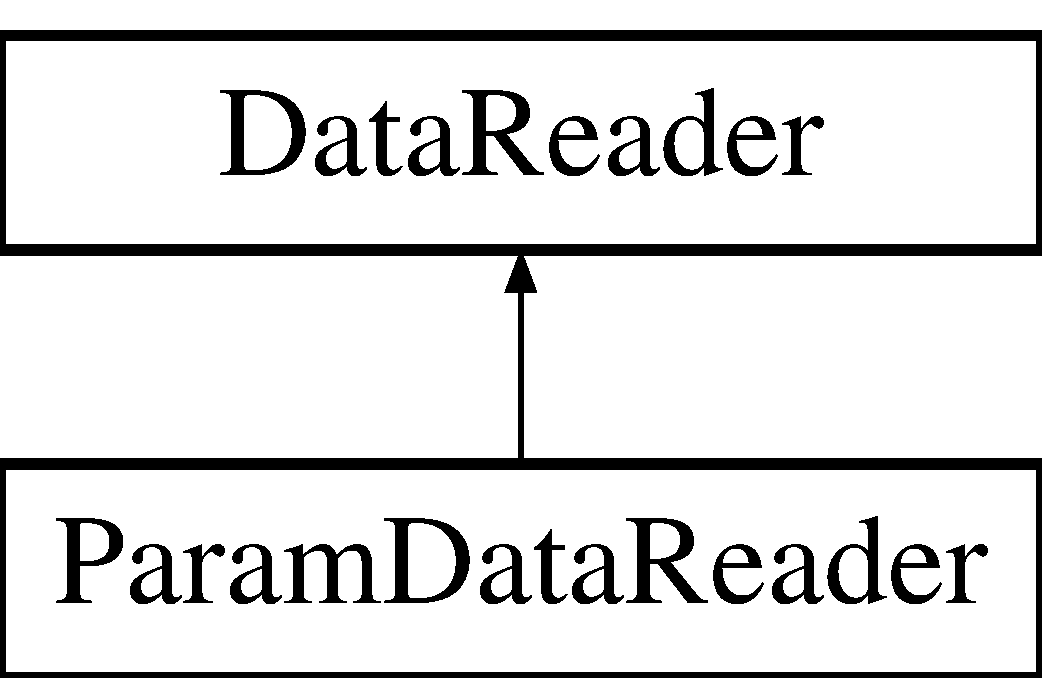
\includegraphics[height=2.000000cm]{classParamDataReader}
\end{center}
\end{figure}
\subsubsection*{Public Member Functions}
\begin{DoxyCompactItemize}
\item 
\hypertarget{classParamDataReader_aae754bb6e204efc6d413fdc714de8e72}{
{\bfseries ParamDataReader} (const std::string \&)}
\label{classParamDataReader_aae754bb6e204efc6d413fdc714de8e72}

\item 
void \hyperlink{classParamDataReader_a6c08000e4e3d408ae14b3146145a1249}{getHeaderRecord} (\hyperlink{structHeaderRecord}{HeaderRecord} \&hdr)
\item 
\hypertarget{classParamDataReader_a505e3e8277b669c56833d64d8d8f291f}{
void {\bfseries getNextEventRecord} (\hyperlink{structHillasParameterization}{HillasParameterization} \&p)}
\label{classParamDataReader_a505e3e8277b669c56833d64d8d8f291f}

\item 
\hypertarget{classParamDataReader_adbedda0f1d3db56c77cfcbb4aa4392e8}{
int {\bfseries size} ()}
\label{classParamDataReader_adbedda0f1d3db56c77cfcbb4aa4392e8}

\item 
\hypertarget{classParamDataReader_afee1c056f8a35d7e1d02a4aecb1ecf6f}{
std::string {\bfseries getTypeString} ()}
\label{classParamDataReader_afee1c056f8a35d7e1d02a4aecb1ecf6f}

\item 
\hypertarget{classParamDataReader_af19fa714276ab64cd02235abd7b0bc93}{
bool {\bfseries isDone} ()}
\label{classParamDataReader_af19fa714276ab64cd02235abd7b0bc93}

\end{DoxyCompactItemize}


\subsubsection{Detailed Description}
Reads parameterized datafiles. 

Definition at line 16 of file ParamDataReader.h.



\subsubsection{Member Function Documentation}
\hypertarget{classParamDataReader_a6c08000e4e3d408ae14b3146145a1249}{
\index{ParamDataReader@{ParamDataReader}!getHeaderRecord@{getHeaderRecord}}
\index{getHeaderRecord@{getHeaderRecord}!ParamDataReader@{ParamDataReader}}
\paragraph[{getHeaderRecord}]{\setlength{\rightskip}{0pt plus 5cm}void ParamDataReader::getHeaderRecord (
\begin{DoxyParamCaption}
\item[{{\bf HeaderRecord} \&}]{hdr}
\end{DoxyParamCaption}
)}}
\label{classParamDataReader_a6c08000e4e3d408ae14b3146145a1249}


Read in the Parameterized header record. 

\begin{Desc}
\item[\hyperlink{todo__todo000023}{Todo}]: should make a ParamHeaderRecord which is a subclass of \hyperlink{structHeaderRecord}{HeaderRecord} which has all the extra parameterized info (like whether zcuts was enabled, etc.) \end{Desc}


Definition at line 82 of file ParamDataReader.cpp.



References HeaderRecord::average\_\-elevation, HeaderRecord::dec, HeaderRecord::endtime, HeaderRecord::nadc, HeaderRecord::num\_\-telescopes, HeaderRecord::ra, HeaderRecord::sourcename, and HeaderRecord::starttime.



Referenced by WUArray::analyzeRun(), and Cutter::cut().



The documentation for this class was generated from the following files:\begin{DoxyCompactItemize}
\item 
ParamDataReader.h\item 
ParamDataReader.cpp\end{DoxyCompactItemize}

\hypertarget{classParamDataWriter}{
\subsection{ParamDataWriter Class Reference}
\label{classParamDataWriter}\index{ParamDataWriter@{ParamDataWriter}}
}


Base class for writing HillasParameterizations to disk.  




{\ttfamily \#include $<$DataWriter.h$>$}

Inheritance diagram for ParamDataWriter:\begin{figure}[H]
\begin{center}
\leavevmode
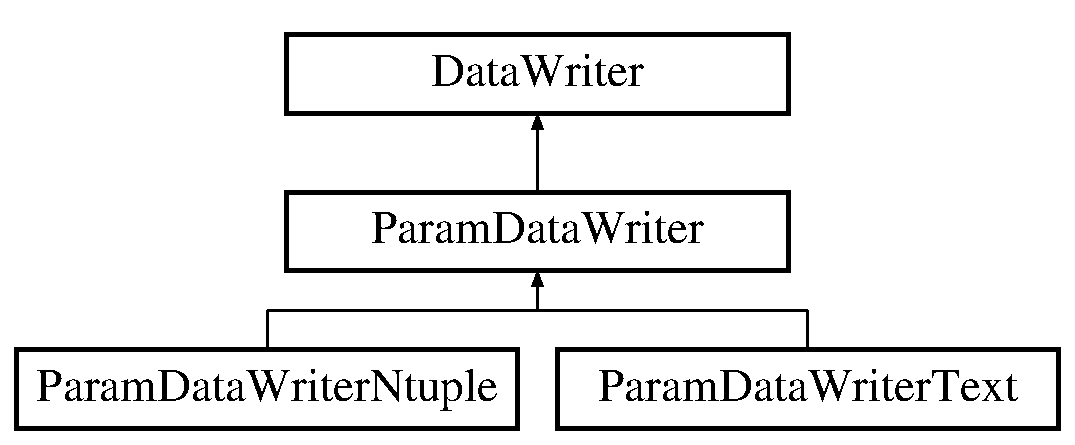
\includegraphics[height=3.000000cm]{classParamDataWriter}
\end{center}
\end{figure}
\subsubsection*{Public Member Functions}
\begin{DoxyCompactItemize}
\item 
\hypertarget{classParamDataWriter_a030c4a57dad508e7767ec321af9a4f2d}{
{\bfseries ParamDataWriter} (const std::string \&filename, bool ow=false)}
\label{classParamDataWriter_a030c4a57dad508e7767ec321af9a4f2d}

\item 
void \hyperlink{classParamDataWriter_a0a70e79b1d085e10036d5a0d437e624b}{writeHeader} (\hyperlink{structHeaderRecord}{HeaderRecord} \&hdr)
\item 
\hypertarget{classParamDataWriter_a35fc7998a33afab877c035eaba013f14}{
virtual void {\bfseries writeParameterization} (\hyperlink{structHillasParameterization}{HillasParameterization} \&param)=0}
\label{classParamDataWriter_a35fc7998a33afab877c035eaba013f14}

\item 
\hypertarget{classParamDataWriter_a6e7ae68618d46d8741fc5ff4b0a5542f}{
virtual void {\bfseries writeParameterization} (\hyperlink{structSimShowerRecord}{SimShowerRecord} \&p1, \hyperlink{structHillasParameterization}{HillasParameterization} \&p2)}
\label{classParamDataWriter_a6e7ae68618d46d8741fc5ff4b0a5542f}

\item 
\hypertarget{classParamDataWriter_a5ea7b99411dd0096a8ee50111b2c193d}{
virtual int {\bfseries size} ()=0}
\label{classParamDataWriter_a5ea7b99411dd0096a8ee50111b2c193d}

\item 
\hypertarget{classParamDataWriter_a65100e91f53c44adb84fd5d541ab7c01}{
virtual std::string {\bfseries getTypeString} ()=0}
\label{classParamDataWriter_a65100e91f53c44adb84fd5d541ab7c01}

\end{DoxyCompactItemize}


\subsubsection{Detailed Description}
Base class for writing HillasParameterizations to disk. 

Subclasses of this should implement the various file formats that can be written. 

Definition at line 41 of file DataWriter.h.



\subsubsection{Member Function Documentation}
\hypertarget{classParamDataWriter_a0a70e79b1d085e10036d5a0d437e624b}{
\index{ParamDataWriter@{ParamDataWriter}!writeHeader@{writeHeader}}
\index{writeHeader@{writeHeader}!ParamDataWriter@{ParamDataWriter}}
\paragraph[{writeHeader}]{\setlength{\rightskip}{0pt plus 5cm}void ParamDataWriter::writeHeader (
\begin{DoxyParamCaption}
\item[{{\bf HeaderRecord} \&}]{hdr}
\end{DoxyParamCaption}
)}}
\label{classParamDataWriter_a0a70e79b1d085e10036d5a0d437e624b}


Write out header. 

Should be done after all NTuple rows have been written, so the number of rows is correct. 

Definition at line 140 of file DataWriter.cpp.



References HeaderRecord::average\_\-elevation, HeaderRecord::dec, HeaderRecord::endtime, HeaderRecord::nadc, HeaderRecord::num\_\-telescopes, HeaderRecord::ra, HeaderRecord::sourcename, and HeaderRecord::starttime.



The documentation for this class was generated from the following files:\begin{DoxyCompactItemize}
\item 
DataWriter.h\item 
DataWriter.cpp\end{DoxyCompactItemize}

\hypertarget{classParamDataWriterNtuple}{
\subsection{ParamDataWriterNtuple Class Reference}
\label{classParamDataWriterNtuple}\index{ParamDataWriterNtuple@{ParamDataWriterNtuple}}
}


Outputs parameterized events to an N-\/Tuple (for use in for example, PAW).  




{\ttfamily \#include $<$DataWriter.h$>$}

Inheritance diagram for ParamDataWriterNtuple:\begin{figure}[H]
\begin{center}
\leavevmode
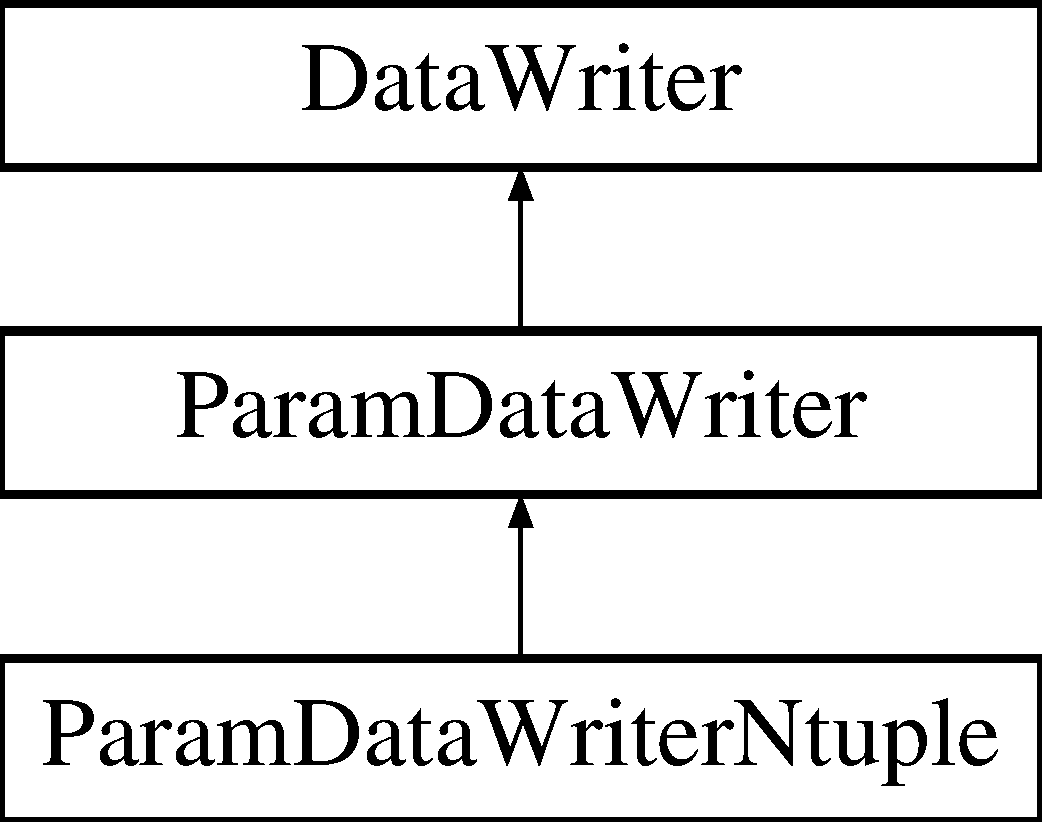
\includegraphics[height=3.000000cm]{classParamDataWriterNtuple}
\end{center}
\end{figure}
\subsubsection*{Public Member Functions}
\begin{DoxyCompactItemize}
\item 
\hypertarget{classParamDataWriterNtuple_a5059611c758f6e6d12b3b31695de0273}{
{\bfseries ParamDataWriterNtuple} (const std::string \&, bool ow=false)}
\label{classParamDataWriterNtuple_a5059611c758f6e6d12b3b31695de0273}

\item 
\hypertarget{classParamDataWriterNtuple_a30e0580d54b007e124dad177cbb367ea}{
void {\bfseries writeParameterization} (\hyperlink{structHillasParameterization}{HillasParameterization} \&)}
\label{classParamDataWriterNtuple_a30e0580d54b007e124dad177cbb367ea}

\item 
\hypertarget{classParamDataWriterNtuple_a8dfa88860127d9b8dbb8537377b4f3e2}{
int {\bfseries size} ()}
\label{classParamDataWriterNtuple_a8dfa88860127d9b8dbb8537377b4f3e2}

\item 
\hypertarget{classParamDataWriterNtuple_a26514c9a723f660f89281fa21cd07c63}{
std::string {\bfseries getTypeString} ()}
\label{classParamDataWriterNtuple_a26514c9a723f660f89281fa21cd07c63}

\end{DoxyCompactItemize}


\subsubsection{Detailed Description}
Outputs parameterized events to an N-\/Tuple (for use in for example, PAW). 

Definition at line 87 of file DataWriter.h.



The documentation for this class was generated from the following files:\begin{DoxyCompactItemize}
\item 
DataWriter.h\item 
DataWriter.cpp\end{DoxyCompactItemize}

\hypertarget{classParamDataWriterText}{
\subsection{ParamDataWriterText Class Reference}
\label{classParamDataWriterText}\index{ParamDataWriterText@{ParamDataWriterText}}
}


Outputs parameterized events to a text file.  




{\ttfamily \#include $<$DataWriter.h$>$}

Inheritance diagram for ParamDataWriterText:\begin{figure}[H]
\begin{center}
\leavevmode
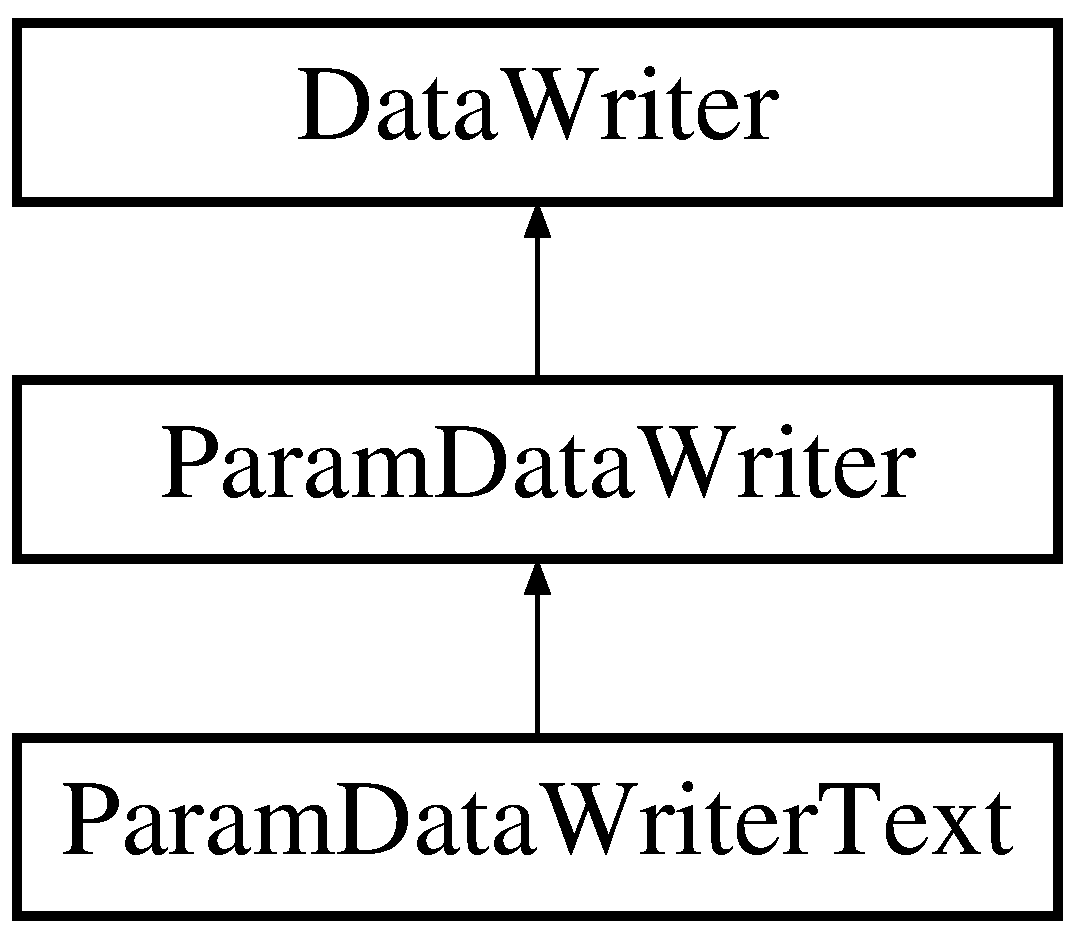
\includegraphics[height=3.000000cm]{classParamDataWriterText}
\end{center}
\end{figure}
\subsubsection*{Public Member Functions}
\begin{DoxyCompactItemize}
\item 
\hypertarget{classParamDataWriterText_a5e5452f5ef2af190c9db883ebd61a556}{
{\bfseries ParamDataWriterText} (const std::string \&, bool ow=false)}
\label{classParamDataWriterText_a5e5452f5ef2af190c9db883ebd61a556}

\item 
\hypertarget{classParamDataWriterText_a7e011f87421ebbdef958b7ba3e952802}{
void {\bfseries writeParameterization} (\hyperlink{structHillasParameterization}{HillasParameterization} \&)}
\label{classParamDataWriterText_a7e011f87421ebbdef958b7ba3e952802}

\item 
\hypertarget{classParamDataWriterText_a1623b4a0a5f2a1bc12b01ace24de91a3}{
void {\bfseries writeParameterization} (\hyperlink{structSimShowerRecord}{SimShowerRecord} \&, \hyperlink{structHillasParameterization}{HillasParameterization} \&)}
\label{classParamDataWriterText_a1623b4a0a5f2a1bc12b01ace24de91a3}

\item 
\hypertarget{classParamDataWriterText_aea625ba1c3132c1dabe138749ae5950a}{
int {\bfseries size} ()}
\label{classParamDataWriterText_aea625ba1c3132c1dabe138749ae5950a}

\item 
\hypertarget{classParamDataWriterText_a56b35c1b1018745bfff6faf757fd58b4}{
std::string {\bfseries getTypeString} ()}
\label{classParamDataWriterText_a56b35c1b1018745bfff6faf757fd58b4}

\end{DoxyCompactItemize}


\subsubsection{Detailed Description}
Outputs parameterized events to a text file. 

Definition at line 63 of file DataWriter.h.



The documentation for this class was generated from the following files:\begin{DoxyCompactItemize}
\item 
DataWriter.h\item 
DataWriter.cpp\end{DoxyCompactItemize}

\hypertarget{classParameterizer}{
\subsection{Parameterizer Class Reference}
\label{classParameterizer}\index{Parameterizer@{Parameterizer}}
}


Contains all functions pretaining to the parameterization of raw data.  




{\ttfamily \#include $<$Parameterizer.h$>$}

\subsubsection*{Classes}
\begin{DoxyCompactItemize}
\item 
struct {\bfseries TelescopeData}
\begin{DoxyCompactList}\small\item\em All per-\/telescope information for the array. \end{DoxyCompactList}\end{DoxyCompactItemize}
\subsubsection*{Public Member Functions}
\begin{DoxyCompactItemize}
\item 
\hypertarget{classParameterizer_ab02d91aaed1db3a62a098d72fd64ea63}{
void \hyperlink{classParameterizer_ab02d91aaed1db3a62a098d72fd64ea63}{process} (\hyperlink{classRunInfo}{RunInfo} \&)}
\label{classParameterizer_ab02d91aaed1db3a62a098d72fd64ea63}

\item 
\hypertarget{classParameterizer_abb53e2c042e188dc22ef4021594a09e5}{
void {\bfseries setLatLonInRadians} (double lat, double lon)}
\label{classParameterizer_abb53e2c042e188dc22ef4021594a09e5}

\item 
\hypertarget{classParameterizer_a9f7704e035f18f73e137c5325dd5e4ca}{
void {\bfseries enableDisplay} (bool val=true)}
\label{classParameterizer_a9f7704e035f18f73e137c5325dd5e4ca}

\item 
\hypertarget{classParameterizer_a872359e61837365be13a236b139b9216}{
void {\bfseries enableVerbose} (bool val=true)}
\label{classParameterizer_a872359e61837365be13a236b139b9216}

\item 
\hypertarget{classParameterizer_a772dc0d2938a0253281b969a7fe0fde7}{
void {\bfseries enableInteractive} (bool val=true)}
\label{classParameterizer_a772dc0d2938a0253281b969a7fe0fde7}

\item 
\hypertarget{classParameterizer_a58cb48804c201ee9f21569aabebef4dc}{
void {\bfseries enableZenithCorrection} (bool val=true)}
\label{classParameterizer_a58cb48804c201ee9f21569aabebef4dc}

\item 
\hypertarget{classParameterizer_aa7997a98c56e52feee7c88d73aeec3c8}{
void {\bfseries enableCleanup} (bool val=true)}
\label{classParameterizer_aa7997a98c56e52feee7c88d73aeec3c8}

\item 
\hypertarget{classParameterizer_a05fe3ca6bc4897005a6b1b63a8c2ee7d}{
void {\bfseries enableOverwrite} (bool val=true)}
\label{classParameterizer_a05fe3ca6bc4897005a6b1b63a8c2ee7d}

\item 
\hypertarget{classParameterizer_a8416f32994c05ffcdf0c27c93ff0d34b}{
void \hyperlink{classParameterizer_a8416f32994c05ffcdf0c27c93ff0d34b}{printSummary} (std::ostream \&stream, \hyperlink{classRunInfo}{RunInfo} \&ri, std::string \&id, \hyperlink{structRawHeaderRecord}{RawHeaderRecord} \&header, \hyperlink{classParamDataWriter}{ParamDataWriter} $\ast$writer, \hyperlink{classRawDataReader}{RawDataReader} $\ast$data, \hyperlink{classTelescopeArray}{TelescopeArray} \&array)}
\label{classParameterizer_a8416f32994c05ffcdf0c27c93ff0d34b}

\end{DoxyCompactItemize}


\subsubsection{Detailed Description}
Contains all functions pretaining to the parameterization of raw data. 

Definition at line 29 of file Parameterizer.h.



The documentation for this class was generated from the following files:\begin{DoxyCompactItemize}
\item 
Parameterizer.h\item 
Parameterizer.cpp\end{DoxyCompactItemize}

\hypertarget{classParamRunInfo}{
\subsection{ParamRunInfo Class Reference}
\label{classParamRunInfo}\index{ParamRunInfo@{ParamRunInfo}}
}


Adds info calculated in the parameterize routine.  




{\ttfamily \#include $<$DataRecords.h$>$}

Inheritance diagram for ParamRunInfo:\begin{figure}[H]
\begin{center}
\leavevmode
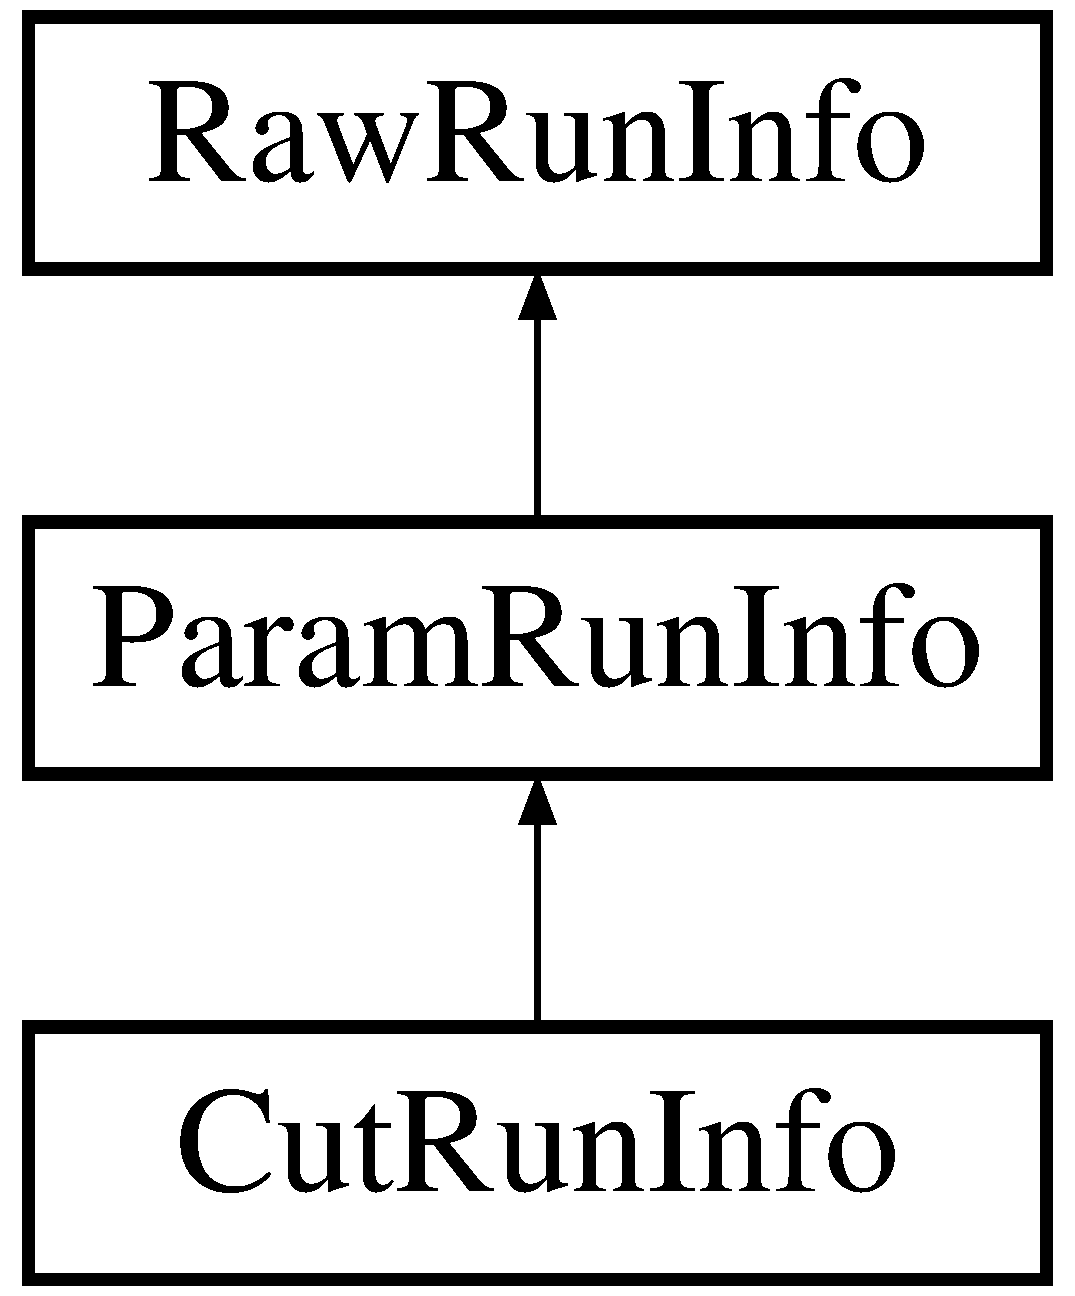
\includegraphics[height=3.000000cm]{classParamRunInfo}
\end{center}
\end{figure}
\subsubsection*{Public Attributes}
\begin{DoxyCompactItemize}
\item 
\hypertarget{classParamRunInfo_af44ec8865cebdc749568d36302e4e900}{
double {\bfseries endtime}}
\label{classParamRunInfo_af44ec8865cebdc749568d36302e4e900}

\item 
\hypertarget{classParamRunInfo_abb72bf8780b2d26bc87fc0796ff35870}{
double {\bfseries average\_\-elevation}}
\label{classParamRunInfo_abb72bf8780b2d26bc87fc0796ff35870}

\end{DoxyCompactItemize}


\subsubsection{Detailed Description}
Adds info calculated in the parameterize routine. 

Definition at line 176 of file DataRecords.h.



The documentation for this class was generated from the following file:\begin{DoxyCompactItemize}
\item 
DataRecords.h\end{DoxyCompactItemize}

\hypertarget{classParseException}{
\subsection{ParseException Class Reference}
\label{classParseException}\index{ParseException@{ParseException}}
}
\subsubsection*{Public Member Functions}
\begin{DoxyCompactItemize}
\item 
\hypertarget{classParseException_a3704bd0b08735099b0f84e10865d2b21}{
{\bfseries ParseException} (string what)}
\label{classParseException_a3704bd0b08735099b0f84e10865d2b21}

\end{DoxyCompactItemize}


\subsubsection{Detailed Description}


Definition at line 37 of file wuplot.cpp.



The documentation for this class was generated from the following file:\begin{DoxyCompactItemize}
\item 
wuplot.cpp\end{DoxyCompactItemize}

\hypertarget{structPedestal}{
\subsection{Pedestal Struct Reference}
\label{structPedestal}\index{Pedestal@{Pedestal}}
}


Contains information about the pedestal for a single tube.  




{\ttfamily \#include $<$PedestalFinder.h$>$}

\subsubsection*{Public Types}
\begin{DoxyCompactItemize}
\item 
enum {\bfseries PEDESTAL\_\-TYPES} \{ {\bfseries GOOD}, 
{\bfseries STAR}, 
{\bfseries TUBEOFF}
 \}
\end{DoxyCompactItemize}
\subsubsection*{Public Attributes}
\begin{DoxyCompactItemize}
\item 
\hypertarget{structPedestal_ab64edfda25e38602732a04e423efc8af}{
double \hyperlink{structPedestal_ab64edfda25e38602732a04e423efc8af}{pedestal}}
\label{structPedestal_ab64edfda25e38602732a04e423efc8af}

\item 
\hypertarget{structPedestal_a5f9004a1267829e05141ae2325e3e420}{
double \hyperlink{structPedestal_a5f9004a1267829e05141ae2325e3e420}{dispersion}}
\label{structPedestal_a5f9004a1267829e05141ae2325e3e420}

\item 
\hypertarget{structPedestal_afd05e3c5f992248f59fe670febeb71fb}{
int \hyperlink{structPedestal_afd05e3c5f992248f59fe670febeb71fb}{type}}
\label{structPedestal_afd05e3c5f992248f59fe670febeb71fb}

\end{DoxyCompactItemize}


\subsubsection{Detailed Description}
Contains information about the pedestal for a single tube. 

Definition at line 15 of file PedestalFinder.h.



The documentation for this struct was generated from the following file:\begin{DoxyCompactItemize}
\item 
PedestalFinder.h\end{DoxyCompactItemize}

\hypertarget{classPedestalFinder}{
\subsection{PedestalFinder Class Reference}
\label{classPedestalFinder}\index{PedestalFinder@{PedestalFinder}}
}


Class to generate pedestal values for a series of runs.  




{\ttfamily \#include $<$PedestalFinder.h$>$}

\subsubsection*{Public Member Functions}
\begin{DoxyCompactItemize}
\item 
\hypertarget{classPedestalFinder_af3f4a0c919666cc2a5caa8f8100a95b2}{
void {\bfseries getOnSourcePeds} (\hyperlink{classRunInfo}{RunInfo} \&ri, std::vector$<$ \hyperlink{structPedestal}{Pedestal} $>$ \&ped, int telescope\_\-id=0)}
\label{classPedestalFinder_af3f4a0c919666cc2a5caa8f8100a95b2}

\item 
\hypertarget{classPedestalFinder_afd22e9acffa21d8be179d53938c93440}{
void {\bfseries getOffSourcePeds} (\hyperlink{classRunInfo}{RunInfo} \&ri, std::vector$<$ \hyperlink{structPedestal}{Pedestal} $>$ \&ped, int telescope\_\-id=0)}
\label{classPedestalFinder_afd22e9acffa21d8be179d53938c93440}

\item 
void \hyperlink{classPedestalFinder_a2f74e3e8ba1b0531f69949adb46d0657}{getPeds} (\hyperlink{classRunInfo}{RunInfo} \&ri, const std::string \&id, std::vector$<$ \hyperlink{structPedestal}{Pedestal} $>$ \&, int telescope\_\-id=0)
\item 
void \hyperlink{classPedestalFinder_add73283676010b81c0730dc22b38437e}{setTubeOffThresholds} (double lower, double upper)
\item 
\hypertarget{classPedestalFinder_a3d77ffa8a2364b28ea29f769620490a6}{
void {\bfseries setBadPedThresh} (double value)}
\label{classPedestalFinder_a3d77ffa8a2364b28ea29f769620490a6}

\end{DoxyCompactItemize}


\subsubsection{Detailed Description}
Class to generate pedestal values for a series of runs. 

Definition at line 29 of file PedestalFinder.h.



\subsubsection{Member Function Documentation}
\hypertarget{classPedestalFinder_a2f74e3e8ba1b0531f69949adb46d0657}{
\index{PedestalFinder@{PedestalFinder}!getPeds@{getPeds}}
\index{getPeds@{getPeds}!PedestalFinder@{PedestalFinder}}
\paragraph[{getPeds}]{\setlength{\rightskip}{0pt plus 5cm}void PedestalFinder::getPeds (
\begin{DoxyParamCaption}
\item[{{\bf RunInfo} \&}]{ri, }
\item[{const std::string \&}]{id, }
\item[{std::vector$<$ {\bf Pedestal} $>$ \&}]{, }
\item[{int}]{telescope\_\-id = {\ttfamily 0}}
\end{DoxyParamCaption}
)}}
\label{classPedestalFinder_a2f74e3e8ba1b0531f69949adb46d0657}


Returns the pedestal values as an array of \hyperlink{structPedestal}{Pedestal} structs. 

\begin{Desc}
\item[\hyperlink{todo__todo000028}{Todo}]: Simulations only contain one pedestal record, so their dispersions are always 0. Due to this, the \hyperlink{classImageCleaner}{ImageCleaner} accepts too many pixels, since it uses the picthresh$\ast$peddisp as the threshold! Need to fix somehow...\end{Desc}


\begin{Desc}
\item[\hyperlink{todo__todo000029}{Todo}]: implement lockfiles to prevent more than one process from writing/reading to the database (necessary for the MPI-\/enabled or a multi-\/threaded version) \end{Desc}


Definition at line 67 of file PedestalFinder.cpp.



References RunInfo::cachedir, RawDataReaderFactory::getReader(), RawDataReaderFactory::instance(), RunInfo::max\_\-ped\_\-events, HeaderRecord::nadc, HeaderRecord::num\_\-telescopes, PlotMaker::plotAxes(), ProgressBar::print(), ProgressBar::printClear(), Logger::printf(), and HeaderRecord::windowsize.



Referenced by GainFinder::getGains().

\hypertarget{classPedestalFinder_add73283676010b81c0730dc22b38437e}{
\index{PedestalFinder@{PedestalFinder}!setTubeOffThresholds@{setTubeOffThresholds}}
\index{setTubeOffThresholds@{setTubeOffThresholds}!PedestalFinder@{PedestalFinder}}
\paragraph[{setTubeOffThresholds}]{\setlength{\rightskip}{0pt plus 5cm}void PedestalFinder::setTubeOffThresholds (
\begin{DoxyParamCaption}
\item[{double}]{lower, }
\item[{double}]{upper}
\end{DoxyParamCaption}
)}}
\label{classPedestalFinder_add73283676010b81c0730dc22b38437e}


Set the thresholds to detect turned off tubes or stars. 


\begin{DoxyParams}{Parameters}
{\em lower} & threshold to detect turned off tubes (default is 0.6) \\
\hline
{\em upper} & threshold to detect stars (default is 1.5) \\
\hline
\end{DoxyParams}


Definition at line 46 of file PedestalFinder.cpp.



Referenced by GainFinder::getGains().



The documentation for this class was generated from the following files:\begin{DoxyCompactItemize}
\item 
PedestalFinder.h\item 
PedestalFinder.cpp\end{DoxyCompactItemize}

\hypertarget{classPlotMaker}{
\subsection{PlotMaker Class Reference}
\label{classPlotMaker}\index{PlotMaker@{PlotMaker}}
}


Plots stuff to any PlotUtils graphics context.  




{\ttfamily \#include $<$PlotMaker.h$>$}

\subsubsection*{Classes}
\begin{DoxyCompactItemize}
\item 
struct {\bfseries PlotState}
\end{DoxyCompactItemize}
\subsubsection*{Public Types}
\begin{DoxyCompactItemize}
\item 
enum {\bfseries ColorMap} \{ \par
{\bfseries COLORMAP\_\-BLUES}, 
{\bfseries COLORMAP\_\-REDBLUE}, 
{\bfseries COLORMAP\_\-YELLOWGREEN}, 
{\bfseries COLORMAP\_\-INVERSEGREY}, 
\par
{\bfseries COLORMAP\_\-GREY}, 
{\bfseries COLORMAP\_\-RAINBOW}, 
{\bfseries COLORMAP\_\-HOT}, 
{\bfseries COLORMAP\_\-PRINTABLE}
 \}
\item 
enum {\bfseries ContourLineStyle} \{ {\bfseries LINE\_\-SOLID}, 
{\bfseries LINE\_\-DOTTED}, 
{\bfseries LINE\_\-DASHED}
 \}
\item 
enum {\bfseries CameraPlotType} \{ {\bfseries CAMERA\_\-IMAGE}, 
{\bfseries CAMERA\_\-PEDS}, 
{\bfseries CAMERA\_\-PEDDISPS}, 
{\bfseries CAMERA\_\-TUBENUMS}
 \}
\end{DoxyCompactItemize}
\subsubsection*{Public Member Functions}
\begin{DoxyCompactItemize}
\item 
\hypertarget{classPlotMaker_ad29eec605eb22329c7b637d565db0834}{
{\bfseries PlotMaker} (std::string type, std::string filename=\char`\"{}\char`\"{}, double minx=-\/3.1, double miny=-\/3.1, double maxx=3.1, double maxy=3.1)}
\label{classPlotMaker_ad29eec605eb22329c7b637d565db0834}

\item 
\hypertarget{classPlotMaker_a27ad38f03afc472ae200ca9cff6bf9c1}{
void {\bfseries setAxisBox} (double minx, double miny, double maxx, double maxy)}
\label{classPlotMaker_a27ad38f03afc472ae200ca9cff6bf9c1}

\item 
\hypertarget{classPlotMaker_ab13a20b6a1bd55ecccf3458cb7c91e9e}{
void {\bfseries setAxisBox} (\hyperlink{classImage2D}{Image2D} \&im2d)}
\label{classPlotMaker_ab13a20b6a1bd55ecccf3458cb7c91e9e}

\item 
\hypertarget{classPlotMaker_ab307012c642e8abfedaa4929999f328d}{
void {\bfseries setAxisBox} (\hyperlink{classCamera}{Camera} \&cam)}
\label{classPlotMaker_ab307012c642e8abfedaa4929999f328d}

\item 
\hypertarget{classPlotMaker_a3a0bd3b9fdd004d19dfeabfd0e0ec4b9}{
void {\bfseries setSpace} (double minx, double miny, double maxx, double maxy)}
\label{classPlotMaker_a3a0bd3b9fdd004d19dfeabfd0e0ec4b9}

\item 
\hypertarget{classPlotMaker_a622cc76bf37733d7b0228b60122afa26}{
void {\bfseries flush} ()}
\label{classPlotMaker_a622cc76bf37733d7b0228b60122afa26}

\item 
\hypertarget{classPlotMaker_a13d5f0523ba4cd8190993643c6e4c6a8}{
void {\bfseries newPage} ()}
\label{classPlotMaker_a13d5f0523ba4cd8190993643c6e4c6a8}

\item 
\hypertarget{classPlotMaker_a7ae7939ed8c5c12f276b431cc861095f}{
void {\bfseries pushState} ()}
\label{classPlotMaker_a7ae7939ed8c5c12f276b431cc861095f}

\item 
\hypertarget{classPlotMaker_a9bec7c4d5b088968228d3f9f1643ed9b}{
void {\bfseries popState} ()}
\label{classPlotMaker_a9bec7c4d5b088968228d3f9f1643ed9b}

\item 
\hypertarget{classPlotMaker_ae7c404f448b8cc74511d551b92458228}{
void {\bfseries rotate} (double theta)}
\label{classPlotMaker_ae7c404f448b8cc74511d551b92458228}

\item 
void \hyperlink{classPlotMaker_a7a63b2f17f113ee6b880aebf1cba1d91}{plotAxes} ()
\item 
\hypertarget{classPlotMaker_a3a11fc277ef5c7d4e930e59c7143b6e7}{
void {\bfseries plotTitle} (std::string title)}
\label{classPlotMaker_a3a11fc277ef5c7d4e930e59c7143b6e7}

\item 
\hypertarget{classPlotMaker_af0b3512703d49e299160fd7b51b279dd}{
void {\bfseries plotSubtitle} (std::string title)}
\label{classPlotMaker_af0b3512703d49e299160fd7b51b279dd}

\item 
\hypertarget{classPlotMaker_a6d5d4f5c931e29e6a86e965db5295a96}{
void {\bfseries plotXTicAt} (double x)}
\label{classPlotMaker_a6d5d4f5c931e29e6a86e965db5295a96}

\item 
\hypertarget{classPlotMaker_a447e61e617e561e98a5ede300966f6d6}{
void {\bfseries plotYTicAt} (double y)}
\label{classPlotMaker_a447e61e617e561e98a5ede300966f6d6}

\item 
\hypertarget{classPlotMaker_ac34e90082c9d8265b635ca22a3ff86b4}{
void {\bfseries plotXMinorTicAt} (double x)}
\label{classPlotMaker_ac34e90082c9d8265b635ca22a3ff86b4}

\item 
\hypertarget{classPlotMaker_a59d9a8f9cc9fe2f147b4ba2afa1d5a30}{
void {\bfseries plotYMinorTicAt} (double y)}
\label{classPlotMaker_a59d9a8f9cc9fe2f147b4ba2afa1d5a30}

\item 
\hypertarget{classPlotMaker_adb2a812fbb301328eb209d1896f7b8fb}{
void \hyperlink{classPlotMaker_adb2a812fbb301328eb209d1896f7b8fb}{contourPlot} (\hyperlink{classImage2D}{Image2D} \&im2d, double zmin, double zmax, double dz)}
\label{classPlotMaker_adb2a812fbb301328eb209d1896f7b8fb}

\item 
\hypertarget{classPlotMaker_ab0317d7d940dff6bee43356cbfebc627}{
void \hyperlink{classPlotMaker_ab0317d7d940dff6bee43356cbfebc627}{plotRADecGrid} (\hyperlink{classImage2D}{Image2D} \&ragrid, \hyperlink{classImage2D}{Image2D} \&decgrid)}
\label{classPlotMaker_ab0317d7d940dff6bee43356cbfebc627}

\item 
\hypertarget{classPlotMaker_a5cd0467a97597f1a9ac7ff56c91e190a}{
void {\bfseries plot} (\hyperlink{classImage2D}{Image2D} \&im2d)}
\label{classPlotMaker_a5cd0467a97597f1a9ac7ff56c91e190a}

\item 
\hypertarget{classPlotMaker_a597669090c5147a8be97852df7bb3ea0}{
void {\bfseries plot} (\hyperlink{classCamera}{Camera} \&cam, const Array\_\-t \&image, const vector$<$ \hyperlink{structPedestal}{Pedestal} $>$ \&peds, vector$<$ int $>$ \&cleanpixels, CameraPlotType plottype=CAMERA\_\-IMAGE)}
\label{classPlotMaker_a597669090c5147a8be97852df7bb3ea0}

\item 
\hypertarget{classPlotMaker_adb38956252f687b85b2bda073004f2b9}{
void {\bfseries plot} (\hyperlink{structHillasParameterization}{HillasParameterization} \&p)}
\label{classPlotMaker_adb38956252f687b85b2bda073004f2b9}

\item 
\hypertarget{classPlotMaker_a58c7f9d496a48d042fe467cf4100275f}{
void {\bfseries plot} (\hyperlink{structMuonParameterization}{MuonParameterization} \&p)}
\label{classPlotMaker_a58c7f9d496a48d042fe467cf4100275f}

\item 
\hypertarget{classPlotMaker_a9c0c99af60541db38461620a9e2c185a}{
void {\bfseries plot} (\hyperlink{classStar}{Star} \&s, int symbol=16)}
\label{classPlotMaker_a9c0c99af60541db38461620a9e2c185a}

\item 
\hypertarget{classPlotMaker_acb86e21bc5d6326aac2d32d074c6dc8d}{
void \hyperlink{classPlotMaker_acb86e21bc5d6326aac2d32d074c6dc8d}{plot} (vector$<$ double $>$ \&xpoints, vector$<$ double $>$ \&ypoints)}
\label{classPlotMaker_acb86e21bc5d6326aac2d32d074c6dc8d}

\item 
\hypertarget{classPlotMaker_a0439c4f4f8961a93286f6daa6a9d29f3}{
void \hyperlink{classPlotMaker_a0439c4f4f8961a93286f6daa6a9d29f3}{plot} (string text, double x, double y)}
\label{classPlotMaker_a0439c4f4f8961a93286f6daa6a9d29f3}

\item 
\hypertarget{classPlotMaker_a43c25aca0a946c325994df24e38700ae}{
void \hyperlink{classPlotMaker_a43c25aca0a946c325994df24e38700ae}{plot} (\hyperlink{classTelescopeArray}{TelescopeArray} \&array)}
\label{classPlotMaker_a43c25aca0a946c325994df24e38700ae}

\item 
\hypertarget{classPlotMaker_a874f1d3b611200fa9b4bccb66262587e}{
void \hyperlink{classPlotMaker_a874f1d3b611200fa9b4bccb66262587e}{plotEllipse} (double x, double y, double r1, double r2, double theta=0)}
\label{classPlotMaker_a874f1d3b611200fa9b4bccb66262587e}

\item 
\hypertarget{classPlotMaker_a66a4d4a2429a768aa46f6e764b660941}{
void {\bfseries plotMarker} (double x, double y)}
\label{classPlotMaker_a66a4d4a2429a768aa46f6e764b660941}

\item 
\hypertarget{classPlotMaker_a979ab6c35a3b71ee86f207e2b6a2e1be}{
void {\bfseries setColorMap} (ColorMap c)}
\label{classPlotMaker_a979ab6c35a3b71ee86f207e2b6a2e1be}

\item 
\hypertarget{classPlotMaker_ac20d8c88996a117e0846346d7ee9fcd3}{
void {\bfseries setColorMap} (string name)}
\label{classPlotMaker_ac20d8c88996a117e0846346d7ee9fcd3}

\item 
void \hyperlink{classPlotMaker_a26f4f8bfb6ed2483617ac8655ff0d05d}{getMappedColor} (double value, int \&red, int \&green, int \&blue)
\item 
\hypertarget{classPlotMaker_a2bd62a359a573a1104ffc8a3f6fceac0}{
void {\bfseries setPixelScale} (double pixscale)}
\label{classPlotMaker_a2bd62a359a573a1104ffc8a3f6fceac0}

\item 
\hypertarget{classPlotMaker_a841b6e3d311ad60bc355dc7802c03735}{
void {\bfseries setScaleFactor} (double factor)}
\label{classPlotMaker_a841b6e3d311ad60bc355dc7802c03735}

\item 
\hypertarget{classPlotMaker_a648464a1b252f30ea8e098bc930c2c69}{
void {\bfseries setTicLevel} (int l)}
\label{classPlotMaker_a648464a1b252f30ea8e098bc930c2c69}

\item 
\hypertarget{classPlotMaker_a6e1ab4682177f627d752c38f7fb4b4a5}{
void {\bfseries setColorScale} (double lower, double upper)}
\label{classPlotMaker_a6e1ab4682177f627d752c38f7fb4b4a5}

\item 
\hypertarget{classPlotMaker_a92d0f21f678e8d97bccf8bfbc3b545a1}{
void {\bfseries enableAutoScale} (bool val=true)}
\label{classPlotMaker_a92d0f21f678e8d97bccf8bfbc3b545a1}

\item 
\hypertarget{classPlotMaker_a94b61535c2bd1bfebabfa9c4d039c0b5}{
void {\bfseries setContourColorName} (string name)}
\label{classPlotMaker_a94b61535c2bd1bfebabfa9c4d039c0b5}

\item 
\hypertarget{classPlotMaker_abf711f48921212a7a8ef89eae1f93b9a}{
void {\bfseries setTicMarkColorName} (string name)}
\label{classPlotMaker_abf711f48921212a7a8ef89eae1f93b9a}

\item 
\hypertarget{classPlotMaker_a8d54078c82180263e11a3e01b8c107b5}{
void {\bfseries setContourLineStyle} (ContourLineStyle i)}
\label{classPlotMaker_a8d54078c82180263e11a3e01b8c107b5}

\item 
\hypertarget{classPlotMaker_af74e3b47a48ae889507344fb3bacae99}{
void {\bfseries setContourLineStyle} (string style)}
\label{classPlotMaker_af74e3b47a48ae889507344fb3bacae99}

\item 
\hypertarget{classPlotMaker_ac92f06122e096dcdfca991043ba86f88}{
void {\bfseries setContourLineWidth} (double width)}
\label{classPlotMaker_ac92f06122e096dcdfca991043ba86f88}

\item 
\hypertarget{classPlotMaker_a22b1936859ca0dc6d16f5fbdab85ae7e}{
void {\bfseries setLabelColorName} (string name)}
\label{classPlotMaker_a22b1936859ca0dc6d16f5fbdab85ae7e}

\item 
\hypertarget{classPlotMaker_af5d99fde6879bdf5895c96e371d08b9a}{
void {\bfseries setLabelAngle} (double theta)}
\label{classPlotMaker_af5d99fde6879bdf5895c96e371d08b9a}

\item 
\hypertarget{classPlotMaker_aee9b0f531899476e0cee2f0904dc1d24}{
void {\bfseries setLabelSize} (double size)}
\label{classPlotMaker_aee9b0f531899476e0cee2f0904dc1d24}

\item 
\hypertarget{classPlotMaker_a826826775cce241941fca3288c3a9a1b}{
void {\bfseries setMarkerType} (int type)}
\label{classPlotMaker_a826826775cce241941fca3288c3a9a1b}

\item 
\hypertarget{classPlotMaker_aefd113e385e3004f653b80043632ca9a}{
void {\bfseries setMarkerSize} (double size)}
\label{classPlotMaker_aefd113e385e3004f653b80043632ca9a}

\item 
\hypertarget{classPlotMaker_a75a64d353ee5b816c9381411fd263c0c}{
void {\bfseries setMarkerColorName} (string name)}
\label{classPlotMaker_a75a64d353ee5b816c9381411fd263c0c}

\end{DoxyCompactItemize}


\subsubsection{Detailed Description}
Plots stuff to any PlotUtils graphics context. 

Definition at line 19 of file PlotMaker.h.



\subsubsection{Member Function Documentation}
\hypertarget{classPlotMaker_a26f4f8bfb6ed2483617ac8655ff0d05d}{
\index{PlotMaker@{PlotMaker}!getMappedColor@{getMappedColor}}
\index{getMappedColor@{getMappedColor}!PlotMaker@{PlotMaker}}
\paragraph[{getMappedColor}]{\setlength{\rightskip}{0pt plus 5cm}void PlotMaker::getMappedColor (
\begin{DoxyParamCaption}
\item[{double}]{value, }
\item[{int \&}]{red, }
\item[{int \&}]{green, }
\item[{int \&}]{blue}
\end{DoxyParamCaption}
)}}
\label{classPlotMaker_a26f4f8bfb6ed2483617ac8655ff0d05d}


Returns the rgb color for the specified grey value (in range 0..1) 


\begin{DoxyParams}{Parameters}
{\em value} & grey value which should be mapped to a color (0..1) \\
\hline
{\em red} & returned color value (0..65535) \\
\hline
{\em green} & returned color value (0..65535) \\
\hline
{\em blue} & returned color value (0..65535) \\
\hline
\end{DoxyParams}


Definition at line 891 of file PlotMaker.cpp.

\hypertarget{classPlotMaker_a7a63b2f17f113ee6b880aebf1cba1d91}{
\index{PlotMaker@{PlotMaker}!plotAxes@{plotAxes}}
\index{plotAxes@{plotAxes}!PlotMaker@{PlotMaker}}
\paragraph[{plotAxes}]{\setlength{\rightskip}{0pt plus 5cm}void PlotMaker::plotAxes (
\begin{DoxyParamCaption}
{}
\end{DoxyParamCaption}
)}}
\label{classPlotMaker_a7a63b2f17f113ee6b880aebf1cba1d91}


Plot a set of axes around the AxisBox region. 

\begin{Desc}
\item[\hyperlink{todo__todo000030}{Todo}]: don't plot minor tics where a major tic is \end{Desc}


Definition at line 98 of file PlotMaker.cpp.



Referenced by WUArray::analyzeRun(), Cutter::cut(), and PedestalFinder::getPeds().



The documentation for this class was generated from the following files:\begin{DoxyCompactItemize}
\item 
PlotMaker.h\item 
PlotMaker.cpp\end{DoxyCompactItemize}

\hypertarget{classProgressBar}{
\subsection{ProgressBar Class Reference}
\label{classProgressBar}\index{ProgressBar@{ProgressBar}}
}


Displays a text-\/based progress bar with estimated time to finish for a particular task.  




{\ttfamily \#include $<$ProgressBar.h$>$}

\subsubsection*{Public Member Functions}
\begin{DoxyCompactItemize}
\item 
\hypertarget{classProgressBar_a2bdc2951819ac35419d55b9dcae74771}{
{\bfseries ProgressBar} (int total, std::string name=\char`\"{}Progress\char`\"{})}
\label{classProgressBar_a2bdc2951819ac35419d55b9dcae74771}

\item 
\hypertarget{classProgressBar_af90db5d2580eadcedddd308f6eb598b7}{
void {\bfseries setName} (std::string name)}
\label{classProgressBar_af90db5d2580eadcedddd308f6eb598b7}

\item 
\hypertarget{classProgressBar_aca2739594eca70b19a8b4c6c8d7b385f}{
void \hyperlink{classProgressBar_aca2739594eca70b19a8b4c6c8d7b385f}{print} (int)}
\label{classProgressBar_aca2739594eca70b19a8b4c6c8d7b385f}

\item 
\hypertarget{classProgressBar_a747aab6ee495c1c07f0fabe5d3e50ec4}{
void \hyperlink{classProgressBar_a747aab6ee495c1c07f0fabe5d3e50ec4}{printClear} ()}
\label{classProgressBar_a747aab6ee495c1c07f0fabe5d3e50ec4}

\item 
\hypertarget{classProgressBar_abcca17e287cdae4b0752e3c7a6428d91}{
double \hyperlink{classProgressBar_abcca17e287cdae4b0752e3c7a6428d91}{getTime} ()}
\label{classProgressBar_abcca17e287cdae4b0752e3c7a6428d91}

\end{DoxyCompactItemize}


\subsubsection{Detailed Description}
Displays a text-\/based progress bar with estimated time to finish for a particular task. 

Definition at line 13 of file ProgressBar.h.



The documentation for this class was generated from the following files:\begin{DoxyCompactItemize}
\item 
ProgressBar.h\item 
ProgressBar.cpp\end{DoxyCompactItemize}

\hypertarget{classRangeException}{
\subsection{RangeException Class Reference}
\label{classRangeException}\index{RangeException@{RangeException}}
}


Thrown by datareaders when the file is over.  




{\ttfamily \#include $<$Exceptions.h$>$}

Inheritance diagram for RangeException:\begin{figure}[H]
\begin{center}
\leavevmode
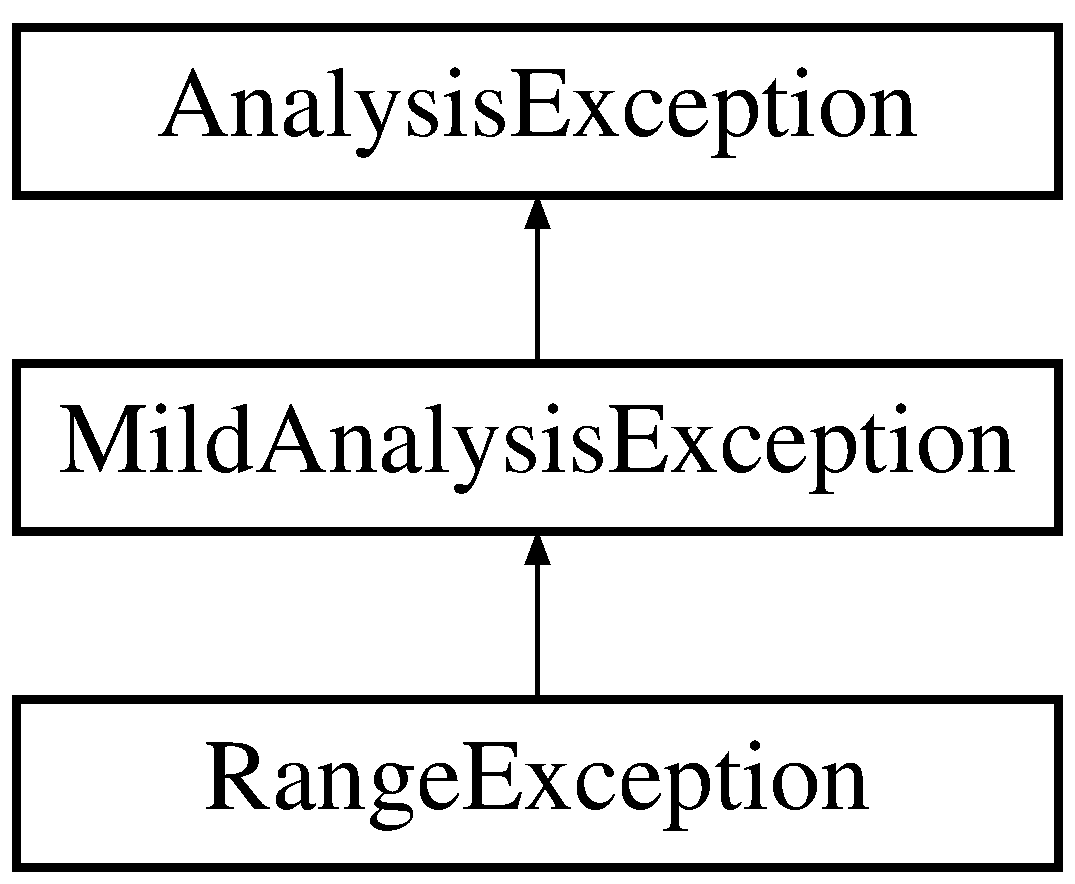
\includegraphics[height=3.000000cm]{classRangeException}
\end{center}
\end{figure}
\subsubsection*{Public Member Functions}
\begin{DoxyCompactItemize}
\item 
\hypertarget{classRangeException_ab269c15c3285c9403089ca022304a809}{
{\bfseries RangeException} (const std::string \&str, int code=0)}
\label{classRangeException_ab269c15c3285c9403089ca022304a809}

\end{DoxyCompactItemize}


\subsubsection{Detailed Description}
Thrown by datareaders when the file is over. 

Definition at line 64 of file Exceptions.h.



The documentation for this class was generated from the following file:\begin{DoxyCompactItemize}
\item 
Exceptions.h\end{DoxyCompactItemize}

\hypertarget{classRawDataReader}{
\subsection{RawDataReader Class Reference}
\label{classRawDataReader}\index{RawDataReader@{RawDataReader}}
}


Reads raw telescope data and produces coresponding records...  




{\ttfamily \#include $<$DataReader.h$>$}

Inheritance diagram for RawDataReader:\begin{figure}[H]
\begin{center}
\leavevmode
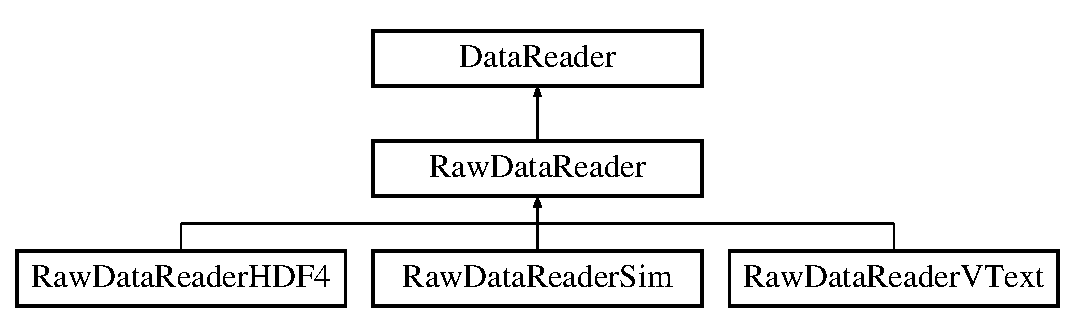
\includegraphics[height=3.000000cm]{classRawDataReader}
\end{center}
\end{figure}
\subsubsection*{Public Types}
\begin{DoxyCompactItemize}
\item 
enum {\bfseries RunType} \{ {\bfseries OTHER}, 
{\bfseries HDF4}, 
{\bfseries SIM}, 
{\bfseries VTEXT}
 \}
\item 
enum {\bfseries EventTypes} \{ {\bfseries EVENT}, 
{\bfseries PEDESTAL}, 
{\bfseries UNKNOWN}
 \}
\end{DoxyCompactItemize}
\subsubsection*{Public Member Functions}
\begin{DoxyCompactItemize}
\item 
\hypertarget{classRawDataReader_a4cf4dcf435e86abd1792be937084d18c}{
{\bfseries RawDataReader} (const std::string \&filename)}
\label{classRawDataReader_a4cf4dcf435e86abd1792be937084d18c}

\item 
\hypertarget{classRawDataReader_aac3ec4c174cb05a97849a1dac8f97571}{
virtual void {\bfseries getHeaderRecord} (\hyperlink{structRawHeaderRecord}{RawHeaderRecord} \&header)=0}
\label{classRawDataReader_aac3ec4c174cb05a97849a1dac8f97571}

\item 
\hypertarget{classRawDataReader_a5d9485d27fba9078f1f4634e1d2349fb}{
virtual void {\bfseries getNextEventRecord} (\hyperlink{structRawEventRecord}{RawEventRecord} \&event)=0}
\label{classRawDataReader_a5d9485d27fba9078f1f4634e1d2349fb}

\item 
\hypertarget{classRawDataReader_a25df0c9abfdfde177c91b0773b4a53c5}{
virtual int {\bfseries size} ()=0}
\label{classRawDataReader_a25df0c9abfdfde177c91b0773b4a53c5}

\item 
\hypertarget{classRawDataReader_ae18f632cbec6ad6267b94da724939700}{
virtual std::string {\bfseries getTypeString} ()=0}
\label{classRawDataReader_ae18f632cbec6ad6267b94da724939700}

\item 
\hypertarget{classRawDataReader_a46d9e42a28ea4cebd6172a87a4e36099}{
virtual int {\bfseries getType} ()=0}
\label{classRawDataReader_a46d9e42a28ea4cebd6172a87a4e36099}

\item 
\hypertarget{classRawDataReader_a203fd47e0b6f43801ccd5de962f24c71}{
virtual bool {\bfseries isDone} ()=0}
\label{classRawDataReader_a203fd47e0b6f43801ccd5de962f24c71}

\end{DoxyCompactItemize}


\subsubsection{Detailed Description}
Reads raw telescope data and produces coresponding records... 

Definition at line 43 of file DataReader.h.



The documentation for this class was generated from the following files:\begin{DoxyCompactItemize}
\item 
DataReader.h\item 
DataReader.cpp\end{DoxyCompactItemize}

\hypertarget{classRawDataReaderFactory}{
\subsection{RawDataReaderFactory Class Reference}
\label{classRawDataReaderFactory}\index{RawDataReaderFactory@{RawDataReaderFactory}}
}


Responsible for locating files and creating the correct data reader object for the detected file type.  




{\ttfamily \#include $<$DataReader.h$>$}

\subsubsection*{Public Member Functions}
\begin{DoxyCompactItemize}
\item 
\hypertarget{classRawDataReaderFactory_ad71f80e5d4c526804c7feedec2368f83}{
\hyperlink{classRawDataReader}{RawDataReader} $\ast$ \hyperlink{classRawDataReaderFactory_ad71f80e5d4c526804c7feedec2368f83}{getReader} (const \hyperlink{classRunInfo}{RunInfo} \&ri, string runid)}
\label{classRawDataReaderFactory_ad71f80e5d4c526804c7feedec2368f83}

\item 
std::string \hyperlink{classRawDataReaderFactory_a3d5b99e24dd4f14a554750b2beb41970}{locateFile} (const \hyperlink{classRunInfo}{RunInfo} \&ri, const string basename, const string ext)
\item 
\hypertarget{classRawDataReaderFactory_a67fb5818c0d0f526c3ac165ada0e5173}{
void \hyperlink{classRawDataReaderFactory_a67fb5818c0d0f526c3ac165ada0e5173}{clearCache} (std::string)}
\label{classRawDataReaderFactory_a67fb5818c0d0f526c3ac165ada0e5173}

\end{DoxyCompactItemize}
\subsubsection*{Static Public Member Functions}
\begin{DoxyCompactItemize}
\item 
\hypertarget{classRawDataReaderFactory_a31ce95b89ad844dfc81a9157ef6ba4e7}{
static \hyperlink{classRawDataReaderFactory}{RawDataReaderFactory} $\ast$ \hyperlink{classRawDataReaderFactory_a31ce95b89ad844dfc81a9157ef6ba4e7}{instance} ()}
\label{classRawDataReaderFactory_a31ce95b89ad844dfc81a9157ef6ba4e7}

\end{DoxyCompactItemize}


\subsubsection{Detailed Description}
Responsible for locating files and creating the correct data reader object for the detected file type. 

Implemented as a Singleton. 

Definition at line 175 of file DataReader.h.



\subsubsection{Member Function Documentation}
\hypertarget{classRawDataReaderFactory_a3d5b99e24dd4f14a554750b2beb41970}{
\index{RawDataReaderFactory@{RawDataReaderFactory}!locateFile@{locateFile}}
\index{locateFile@{locateFile}!RawDataReaderFactory@{RawDataReaderFactory}}
\paragraph[{locateFile}]{\setlength{\rightskip}{0pt plus 5cm}string RawDataReaderFactory::locateFile (
\begin{DoxyParamCaption}
\item[{const {\bf RunInfo} \&}]{ri, }
\item[{const string}]{basename, }
\item[{const string}]{ext}
\end{DoxyParamCaption}
)}}
\label{classRawDataReaderFactory_a3d5b99e24dd4f14a554750b2beb41970}


Locate a file in a directory structure, uncompressing if needed. 


\begin{DoxyParams}{Parameters}
{\em startdir} & directory under which to look \\
\hline
{\em basename} & base name of the file (without extensions) \\
\hline
{\em file} & extension (i.e. hdf)\\
\hline
\end{DoxyParams}
\begin{DoxyReturn}{Returns}
full pathname to the located file. 
\end{DoxyReturn}


Definition at line 773 of file DataReader.cpp.



References RunInfo::cachedir, and RunInfo::datadir.



Referenced by getReader().



The documentation for this class was generated from the following files:\begin{DoxyCompactItemize}
\item 
DataReader.h\item 
DataReader.cpp\end{DoxyCompactItemize}

\hypertarget{classRawDataReaderHDF4}{
\subsection{RawDataReaderHDF4 Class Reference}
\label{classRawDataReaderHDF4}\index{RawDataReaderHDF4@{RawDataReaderHDF4}}
}


Implementation of \hyperlink{classRawDataReader}{RawDataReader} for HDF4 input files.  




{\ttfamily \#include $<$DataReader.h$>$}

Inheritance diagram for RawDataReaderHDF4:\begin{figure}[H]
\begin{center}
\leavevmode
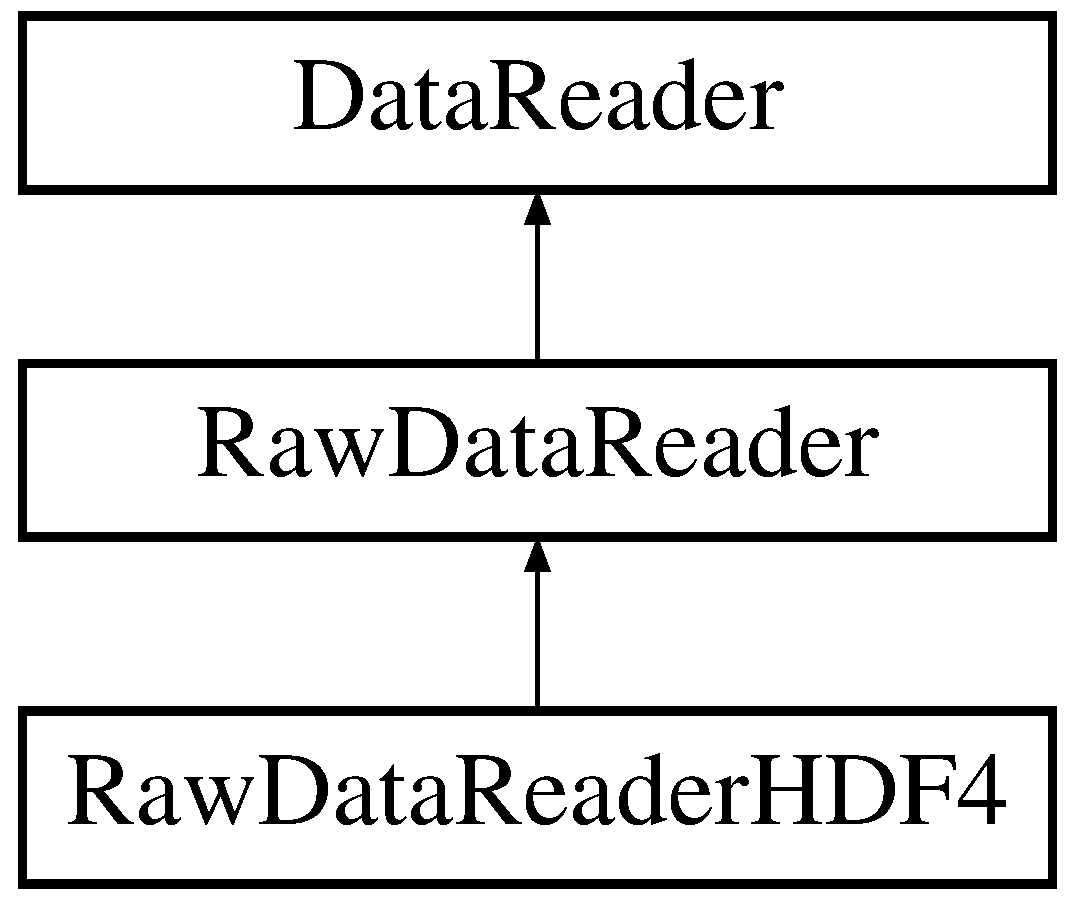
\includegraphics[height=3.000000cm]{classRawDataReaderHDF4}
\end{center}
\end{figure}
\subsubsection*{Public Member Functions}
\begin{DoxyCompactItemize}
\item 
\hypertarget{classRawDataReaderHDF4_a5b37d2a4ff84f6eed2da5f1de561375a}{
{\bfseries RawDataReaderHDF4} (const std::string \&filename)}
\label{classRawDataReaderHDF4_a5b37d2a4ff84f6eed2da5f1de561375a}

\item 
\hypertarget{classRawDataReaderHDF4_a22b736687a2a4457faad3c81504e25b2}{
void {\bfseries getHeaderRecord} (\hyperlink{structRawHeaderRecord}{RawHeaderRecord} \&header)}
\label{classRawDataReaderHDF4_a22b736687a2a4457faad3c81504e25b2}

\item 
\hypertarget{classRawDataReaderHDF4_a653b654370668e69836da44befccb3f1}{
void {\bfseries getNextEventRecord} (\hyperlink{structRawEventRecord}{RawEventRecord} \&event)}
\label{classRawDataReaderHDF4_a653b654370668e69836da44befccb3f1}

\item 
\hypertarget{classRawDataReaderHDF4_a70f0b243aec5ed6d33eb6e2878a07046}{
int \hyperlink{classRawDataReaderHDF4_a70f0b243aec5ed6d33eb6e2878a07046}{size} ()}
\label{classRawDataReaderHDF4_a70f0b243aec5ed6d33eb6e2878a07046}

\item 
\hypertarget{classRawDataReaderHDF4_aca39621e50d5b60f6918935f7a9b32be}{
bool {\bfseries isDone} ()}
\label{classRawDataReaderHDF4_aca39621e50d5b60f6918935f7a9b32be}

\item 
\hypertarget{classRawDataReaderHDF4_a936c6a127b504b118d67c04b5d9bace3}{
std::string {\bfseries getTypeString} ()}
\label{classRawDataReaderHDF4_a936c6a127b504b118d67c04b5d9bace3}

\item 
\hypertarget{classRawDataReaderHDF4_ab32ddb7a12206ef68fec23714bc9b9ac}{
int {\bfseries getType} ()}
\label{classRawDataReaderHDF4_ab32ddb7a12206ef68fec23714bc9b9ac}

\end{DoxyCompactItemize}


\subsubsection{Detailed Description}
Implementation of \hyperlink{classRawDataReader}{RawDataReader} for HDF4 input files. 

Definition at line 68 of file DataReader.h.



The documentation for this class was generated from the following files:\begin{DoxyCompactItemize}
\item 
DataReader.h\item 
DataReader.cpp\end{DoxyCompactItemize}

\hypertarget{classRawDataReaderSim}{
\subsection{RawDataReaderSim Class Reference}
\label{classRawDataReaderSim}\index{RawDataReaderSim@{RawDataReaderSim}}
}


Implementation of \hyperlink{classRawDataReader}{RawDataReader} for simulation .tubes files.  




{\ttfamily \#include $<$DataReader.h$>$}

Inheritance diagram for RawDataReaderSim:\begin{figure}[H]
\begin{center}
\leavevmode
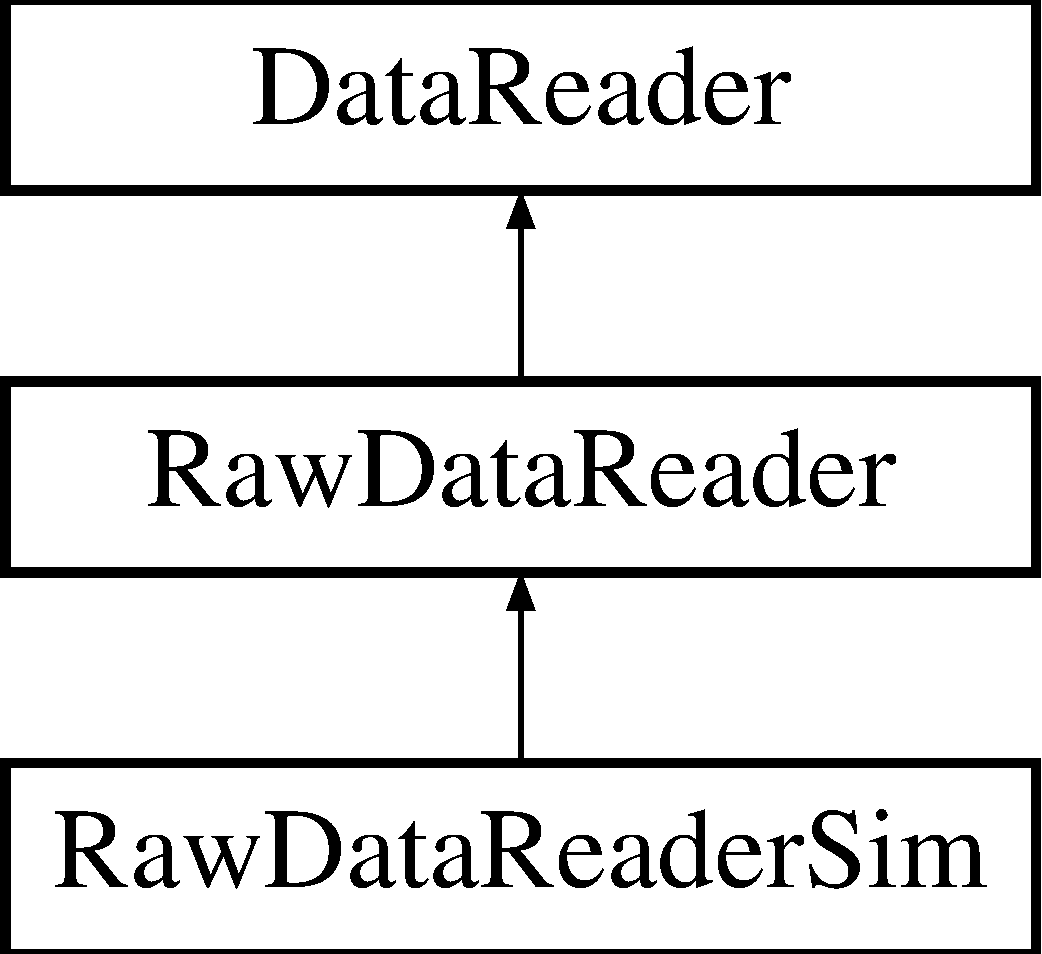
\includegraphics[height=3.000000cm]{classRawDataReaderSim}
\end{center}
\end{figure}
\subsubsection*{Public Member Functions}
\begin{DoxyCompactItemize}
\item 
\hyperlink{classRawDataReaderSim_a3b39f633634f97e2962f80f2c60bf8b0}{RawDataReaderSim} (const std::string \&filename)
\item 
void \hyperlink{classRawDataReaderSim_acd4f407d9c8b8df95eb88213e6625f5f}{getHeaderRecord} (\hyperlink{structRawHeaderRecord}{RawHeaderRecord} \&header)
\item 
\hypertarget{classRawDataReaderSim_af7c83e5db612afd37d2e0daeecb33e32}{
void \hyperlink{classRawDataReaderSim_af7c83e5db612afd37d2e0daeecb33e32}{getNextEventRecord} (\hyperlink{structRawEventRecord}{RawEventRecord} \&event)}
\label{classRawDataReaderSim_af7c83e5db612afd37d2e0daeecb33e32}

\item 
\hypertarget{classRawDataReaderSim_aedc584c28c0b04a8ddeedf2680cd316f}{
int \hyperlink{classRawDataReaderSim_aedc584c28c0b04a8ddeedf2680cd316f}{size} ()}
\label{classRawDataReaderSim_aedc584c28c0b04a8ddeedf2680cd316f}

\item 
\hypertarget{classRawDataReaderSim_a97dae8ae36836c8a7ad8da1600cf3319}{
bool {\bfseries isDone} ()}
\label{classRawDataReaderSim_a97dae8ae36836c8a7ad8da1600cf3319}

\item 
\hypertarget{classRawDataReaderSim_aa7ab2d94ea9b7b87db0f1a83d3b592ff}{
std::string {\bfseries getTypeString} ()}
\label{classRawDataReaderSim_aa7ab2d94ea9b7b87db0f1a83d3b592ff}

\item 
\hypertarget{classRawDataReaderSim_abcd7b3c9361abd1efb9064945844d06e}{
int {\bfseries getType} ()}
\label{classRawDataReaderSim_abcd7b3c9361abd1efb9064945844d06e}

\item 
\hypertarget{classRawDataReaderSim_ac03bf61391a4d740f91f5905bb3cf7c1}{
\hyperlink{structSimShowerRecord}{SimShowerRecord} {\bfseries getSimShowerRecord} ()}
\label{classRawDataReaderSim_ac03bf61391a4d740f91f5905bb3cf7c1}

\end{DoxyCompactItemize}


\subsubsection{Detailed Description}
Implementation of \hyperlink{classRawDataReader}{RawDataReader} for simulation .tubes files. 

Definition at line 104 of file DataReader.h.



\subsubsection{Constructor \& Destructor Documentation}
\hypertarget{classRawDataReaderSim_a3b39f633634f97e2962f80f2c60bf8b0}{
\index{RawDataReaderSim@{RawDataReaderSim}!RawDataReaderSim@{RawDataReaderSim}}
\index{RawDataReaderSim@{RawDataReaderSim}!RawDataReaderSim@{RawDataReaderSim}}
\paragraph[{RawDataReaderSim}]{\setlength{\rightskip}{0pt plus 5cm}RawDataReaderSim::RawDataReaderSim (
\begin{DoxyParamCaption}
\item[{const std::string \&}]{filename}
\end{DoxyParamCaption}
)}}
\label{classRawDataReaderSim_a3b39f633634f97e2962f80f2c60bf8b0}


Open .rec input file. 

\begin{Desc}
\item[\hyperlink{bug__bug000001}{Bug}]: if file doesn't exist, doesn't always fail! \end{Desc}


Definition at line 297 of file DataReader.cpp.



\subsubsection{Member Function Documentation}
\hypertarget{classRawDataReaderSim_acd4f407d9c8b8df95eb88213e6625f5f}{
\index{RawDataReaderSim@{RawDataReaderSim}!getHeaderRecord@{getHeaderRecord}}
\index{getHeaderRecord@{getHeaderRecord}!RawDataReaderSim@{RawDataReaderSim}}
\paragraph[{getHeaderRecord}]{\setlength{\rightskip}{0pt plus 5cm}void RawDataReaderSim::getHeaderRecord (
\begin{DoxyParamCaption}
\item[{{\bf RawHeaderRecord} \&}]{header}
\end{DoxyParamCaption}
)\hspace{0.3cm}{\ttfamily  \mbox{[}virtual\mbox{]}}}}
\label{classRawDataReaderSim_acd4f407d9c8b8df95eb88213e6625f5f}


Get header record. 

\begin{Desc}
\item[\hyperlink{todo__todo000008}{Todo}]: fill in the correct values \end{Desc}


Implements \hyperlink{classRawDataReader}{RawDataReader}.



Definition at line 344 of file DataReader.cpp.



References HeaderRecord::dec, HeaderRecord::nadc, HeaderRecord::ra, HeaderRecord::sourcename, and HeaderRecord::starttime.



The documentation for this class was generated from the following files:\begin{DoxyCompactItemize}
\item 
DataReader.h\item 
DataReader.cpp\end{DoxyCompactItemize}

\hypertarget{classRawDataReaderVText}{
\subsection{RawDataReaderVText Class Reference}
\label{classRawDataReaderVText}\index{RawDataReaderVText@{RawDataReaderVText}}
}


Implementation of \hyperlink{classRawDataReader}{RawDataReader} VERITAS text data as outputed by Paul Rebillot's charge integration routines.  




{\ttfamily \#include $<$DataReader.h$>$}

Inheritance diagram for RawDataReaderVText:\begin{figure}[H]
\begin{center}
\leavevmode
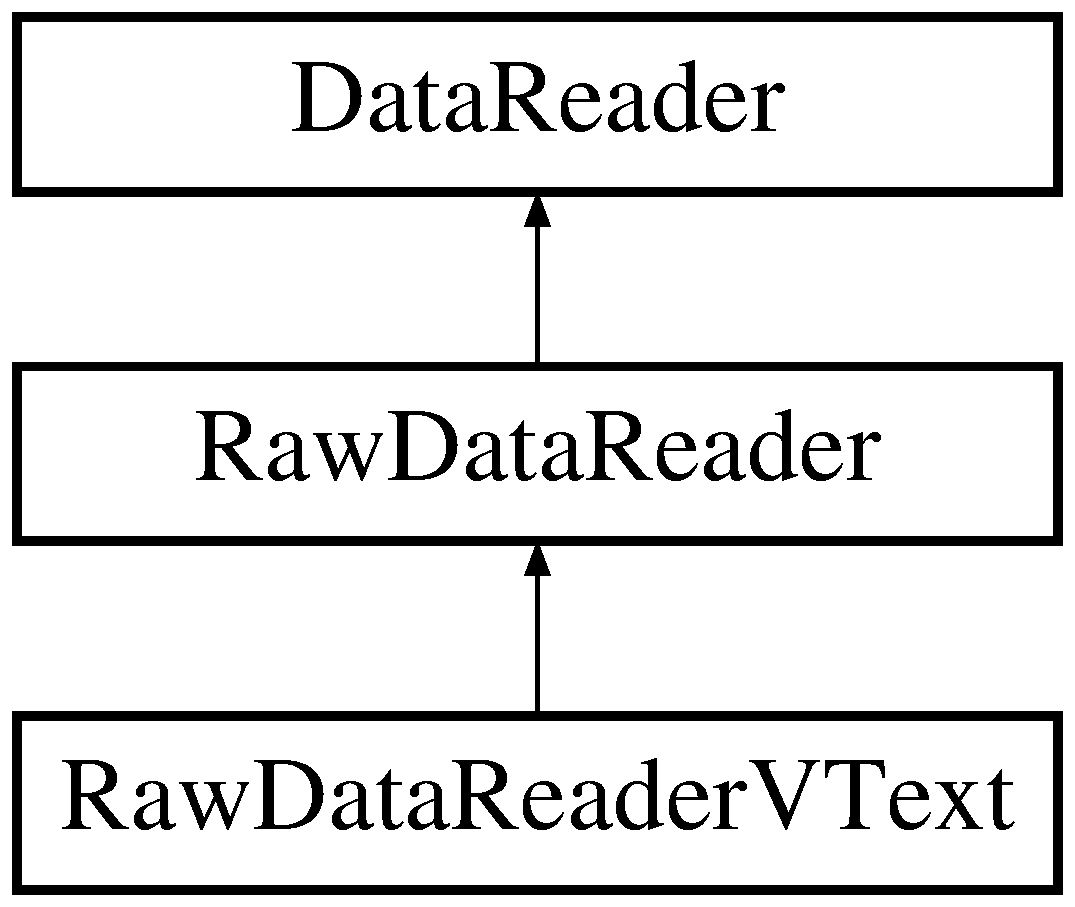
\includegraphics[height=3.000000cm]{classRawDataReaderVText}
\end{center}
\end{figure}
\subsubsection*{Public Member Functions}
\begin{DoxyCompactItemize}
\item 
\hypertarget{classRawDataReaderVText_a88870b1f83b0348a399052fea589c9df}{
\hyperlink{classRawDataReaderVText_a88870b1f83b0348a399052fea589c9df}{RawDataReaderVText} (const std::string \&filename)}
\label{classRawDataReaderVText_a88870b1f83b0348a399052fea589c9df}

\item 
void \hyperlink{classRawDataReaderVText_a7fb3e50fa41df971c06c1b424c713675}{getHeaderRecord} (\hyperlink{structRawHeaderRecord}{RawHeaderRecord} \&header)
\item 
void \hyperlink{classRawDataReaderVText_aba47308e73a41331cff56a3b38109a17}{getNextEventRecord} (\hyperlink{structRawEventRecord}{RawEventRecord} \&event)
\item 
\hypertarget{classRawDataReaderVText_adca172216ac8835629493b3c5845f952}{
int \hyperlink{classRawDataReaderVText_adca172216ac8835629493b3c5845f952}{size} ()}
\label{classRawDataReaderVText_adca172216ac8835629493b3c5845f952}

\item 
\hypertarget{classRawDataReaderVText_a7049b224eb00a191a520070ae4558521}{
bool {\bfseries isDone} ()}
\label{classRawDataReaderVText_a7049b224eb00a191a520070ae4558521}

\item 
\hypertarget{classRawDataReaderVText_a7e68f833fba61cb69358cb751b83a2bf}{
std::string {\bfseries getTypeString} ()}
\label{classRawDataReaderVText_a7e68f833fba61cb69358cb751b83a2bf}

\item 
\hypertarget{classRawDataReaderVText_adaa1bd5162aeaa1430036dd84981051f}{
int {\bfseries getType} ()}
\label{classRawDataReaderVText_adaa1bd5162aeaa1430036dd84981051f}

\end{DoxyCompactItemize}


\subsubsection{Detailed Description}
Implementation of \hyperlink{classRawDataReader}{RawDataReader} VERITAS text data as outputed by Paul Rebillot's charge integration routines. 

Definition at line 138 of file DataReader.h.



\subsubsection{Member Function Documentation}
\hypertarget{classRawDataReaderVText_a7fb3e50fa41df971c06c1b424c713675}{
\index{RawDataReaderVText@{RawDataReaderVText}!getHeaderRecord@{getHeaderRecord}}
\index{getHeaderRecord@{getHeaderRecord}!RawDataReaderVText@{RawDataReaderVText}}
\paragraph[{getHeaderRecord}]{\setlength{\rightskip}{0pt plus 5cm}void RawDataReaderVText::getHeaderRecord (
\begin{DoxyParamCaption}
\item[{{\bf RawHeaderRecord} \&}]{header}
\end{DoxyParamCaption}
)\hspace{0.3cm}{\ttfamily  \mbox{[}virtual\mbox{]}}}}
\label{classRawDataReaderVText_a7fb3e50fa41df971c06c1b424c713675}


Get header record. 

\begin{Desc}
\item[\hyperlink{todo__todo000009}{Todo}]: fill in the correct values \end{Desc}


Implements \hyperlink{classRawDataReader}{RawDataReader}.



Definition at line 497 of file DataReader.cpp.



References HeaderRecord::dec, HeaderRecord::nadc, HeaderRecord::num\_\-telescopes, HeaderRecord::ra, HeaderRecord::sourcename, HeaderRecord::starttime, and HeaderRecord::windowsize.



Referenced by size().

\hypertarget{classRawDataReaderVText_aba47308e73a41331cff56a3b38109a17}{
\index{RawDataReaderVText@{RawDataReaderVText}!getNextEventRecord@{getNextEventRecord}}
\index{getNextEventRecord@{getNextEventRecord}!RawDataReaderVText@{RawDataReaderVText}}
\paragraph[{getNextEventRecord}]{\setlength{\rightskip}{0pt plus 5cm}void RawDataReaderVText::getNextEventRecord (
\begin{DoxyParamCaption}
\item[{{\bf RawEventRecord} \&}]{event}
\end{DoxyParamCaption}
)\hspace{0.3cm}{\ttfamily  \mbox{[}virtual\mbox{]}}}}
\label{classRawDataReaderVText_aba47308e73a41331cff56a3b38109a17}


Returns the next \hyperlink{structRawEventRecord}{RawEventRecord} from the simulation. 

format is: type event\_\-num gpstime osctime livetime elevation azimuth telescope\_\-id adcvalues\mbox{[}499\mbox{]} 

Implements \hyperlink{classRawDataReader}{RawDataReader}.



Definition at line 571 of file DataReader.cpp.



The documentation for this class was generated from the following files:\begin{DoxyCompactItemize}
\item 
DataReader.h\item 
DataReader.cpp\end{DoxyCompactItemize}

\hypertarget{structRawEventRecord}{
\subsection{RawEventRecord Struct Reference}
\label{structRawEventRecord}\index{RawEventRecord@{RawEventRecord}}
}


One event from a raw data file.  




{\ttfamily \#include $<$DataRecords.h$>$}

Inheritance diagram for RawEventRecord:\begin{figure}[H]
\begin{center}
\leavevmode
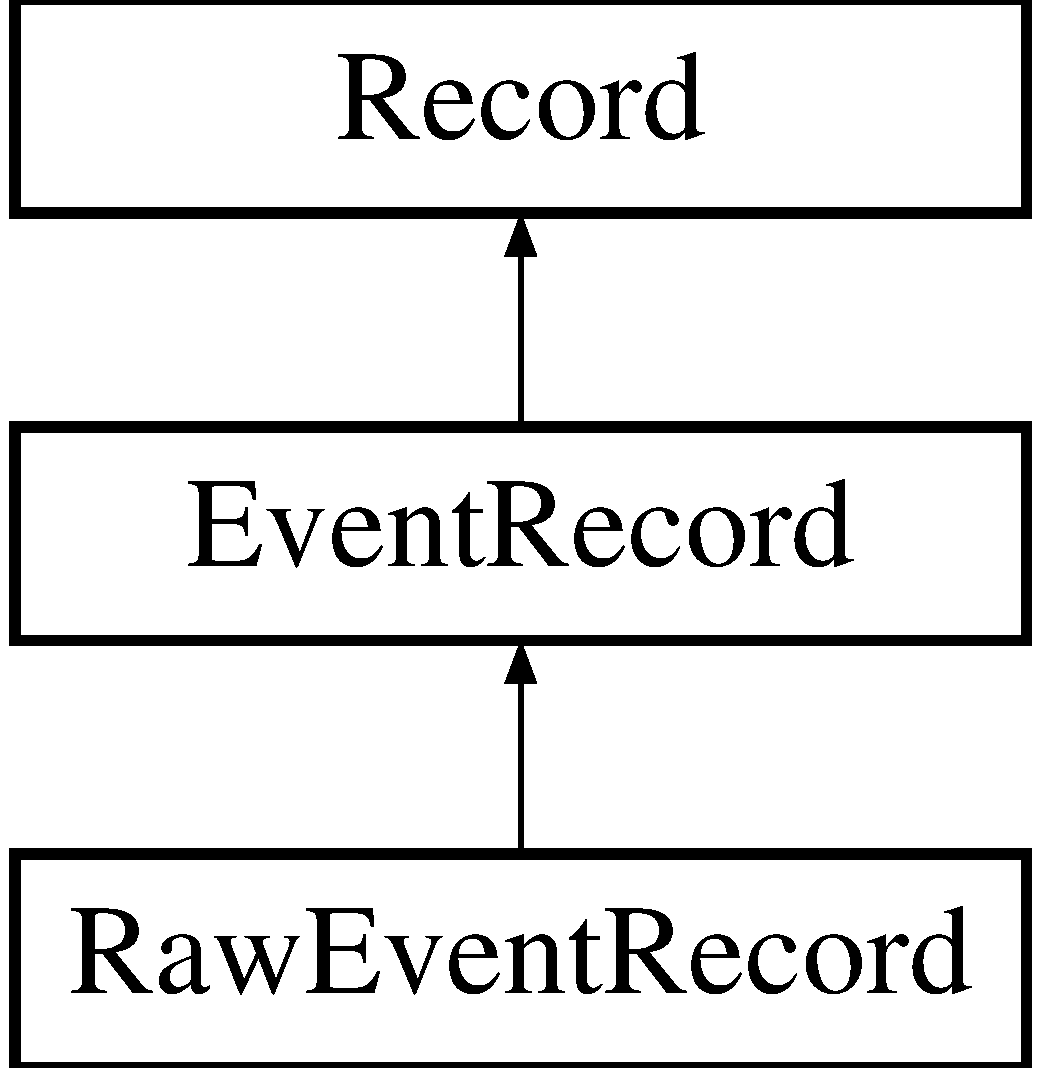
\includegraphics[height=3.000000cm]{structRawEventRecord}
\end{center}
\end{figure}
\subsubsection*{Public Attributes}
\begin{DoxyCompactItemize}
\item 
\hypertarget{structRawEventRecord_acc7886a2fb11a6bfb9132879afb079c8}{
int {\bfseries type}}
\label{structRawEventRecord_acc7886a2fb11a6bfb9132879afb079c8}

\item 
\hypertarget{structRawEventRecord_aeed99c02bce8a12e4fac3956ca0b503d}{
double {\bfseries gpstime}}
\label{structRawEventRecord_aeed99c02bce8a12e4fac3956ca0b503d}

\item 
\hypertarget{structRawEventRecord_a7a3855135e75162d6cc56cc660c9a310}{
double {\bfseries osctime}}
\label{structRawEventRecord_a7a3855135e75162d6cc56cc660c9a310}

\item 
\hypertarget{structRawEventRecord_ae9dca8bc5831835b45564247f8d710fb}{
double {\bfseries livetime}}
\label{structRawEventRecord_ae9dca8bc5831835b45564247f8d710fb}

\item 
\hypertarget{structRawEventRecord_afa1d6ff6df7b0edfd9d1585eaa6f5eee}{
short {\bfseries elevation}}
\label{structRawEventRecord_afa1d6ff6df7b0edfd9d1585eaa6f5eee}

\item 
\hypertarget{structRawEventRecord_a827becd5b6d801ff65bd867c7654a268}{
short {\bfseries azimuth}}
\label{structRawEventRecord_a827becd5b6d801ff65bd867c7654a268}

\item 
\hypertarget{structRawEventRecord_ae6253089b2c41e82020c6c4df0e903be}{
int {\bfseries telescope\_\-id}}
\label{structRawEventRecord_ae6253089b2c41e82020c6c4df0e903be}

\item 
\hypertarget{structRawEventRecord_abd20470e19dc3881c103a5875fe81c52}{
Array\_\-t {\bfseries adc}}
\label{structRawEventRecord_abd20470e19dc3881c103a5875fe81c52}

\end{DoxyCompactItemize}


\subsubsection{Detailed Description}
One event from a raw data file. 

Definition at line 68 of file DataRecords.h.



The documentation for this struct was generated from the following file:\begin{DoxyCompactItemize}
\item 
DataRecords.h\end{DoxyCompactItemize}

\hypertarget{structRawHeaderRecord}{
\subsection{RawHeaderRecord Struct Reference}
\label{structRawHeaderRecord}\index{RawHeaderRecord@{RawHeaderRecord}}
}
Inheritance diagram for RawHeaderRecord:\begin{figure}[H]
\begin{center}
\leavevmode
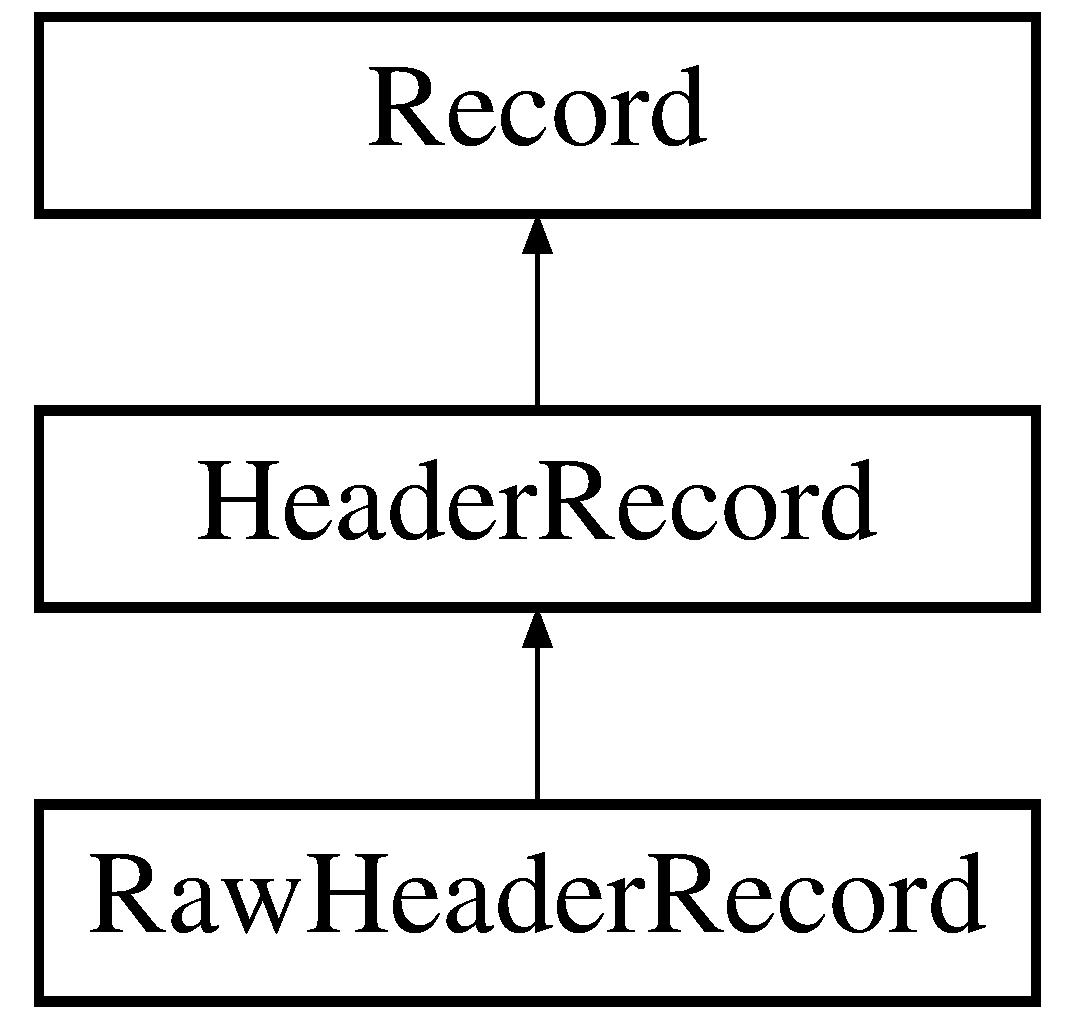
\includegraphics[height=3.000000cm]{structRawHeaderRecord}
\end{center}
\end{figure}


\subsubsection{Detailed Description}


Definition at line 83 of file DataRecords.h.



The documentation for this struct was generated from the following file:\begin{DoxyCompactItemize}
\item 
DataRecords.h\end{DoxyCompactItemize}

\hypertarget{classRawRunInfo}{
\subsection{RawRunInfo Class Reference}
\label{classRawRunInfo}\index{RawRunInfo@{RawRunInfo}}
}


Header Information read from the raw data.  




{\ttfamily \#include $<$DataRecords.h$>$}

Inheritance diagram for RawRunInfo:\begin{figure}[H]
\begin{center}
\leavevmode
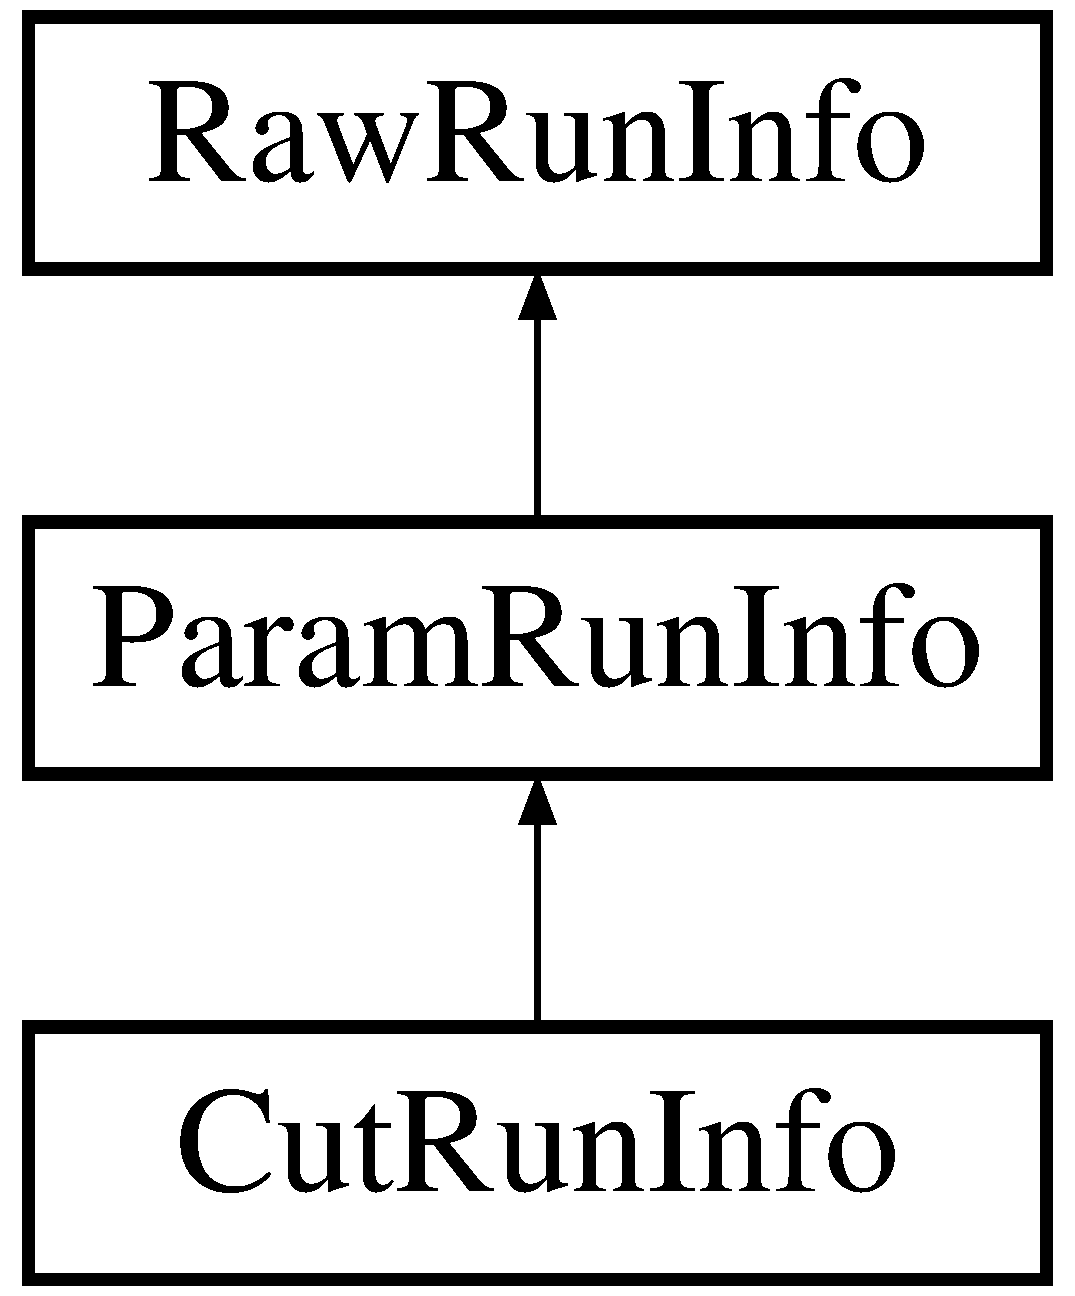
\includegraphics[height=3.000000cm]{classRawRunInfo}
\end{center}
\end{figure}
\subsubsection*{Public Attributes}
\begin{DoxyCompactItemize}
\item 
\hypertarget{classRawRunInfo_a6e8ce531367afe08e6410a1112cf9239}{
std::string {\bfseries sourcename}}
\label{classRawRunInfo_a6e8ce531367afe08e6410a1112cf9239}

\item 
\hypertarget{classRawRunInfo_a8da01ce0afd73527dc533cd0ca53052c}{
std::string {\bfseries runid}}
\label{classRawRunInfo_a8da01ce0afd73527dc533cd0ca53052c}

\item 
\hypertarget{classRawRunInfo_a5f6b4e860d51518b7761ec06aeff550f}{
int {\bfseries nadc}}
\label{classRawRunInfo_a5f6b4e860d51518b7761ec06aeff550f}

\item 
\hypertarget{classRawRunInfo_a1f43e3129e80774302a5df71134ee57f}{
double {\bfseries ra}}
\label{classRawRunInfo_a1f43e3129e80774302a5df71134ee57f}

\item 
\hypertarget{classRawRunInfo_ac8d167b878630455968ebda6c27a4b56}{
double {\bfseries dec}}
\label{classRawRunInfo_ac8d167b878630455968ebda6c27a4b56}

\item 
\hypertarget{classRawRunInfo_a4a0fcbbbdc91a8382b9e30cf9f3caba4}{
double {\bfseries starttime}}
\label{classRawRunInfo_a4a0fcbbbdc91a8382b9e30cf9f3caba4}

\end{DoxyCompactItemize}


\subsubsection{Detailed Description}
Header Information read from the raw data. 

Definition at line 161 of file DataRecords.h.



The documentation for this class was generated from the following file:\begin{DoxyCompactItemize}
\item 
DataRecords.h\end{DoxyCompactItemize}

\hypertarget{structRecord}{
\subsection{Record Struct Reference}
\label{structRecord}\index{Record@{Record}}
}


Records are readable/writable (i.e.  




{\ttfamily \#include $<$DataRecords.h$>$}

Inheritance diagram for Record:\begin{figure}[H]
\begin{center}
\leavevmode
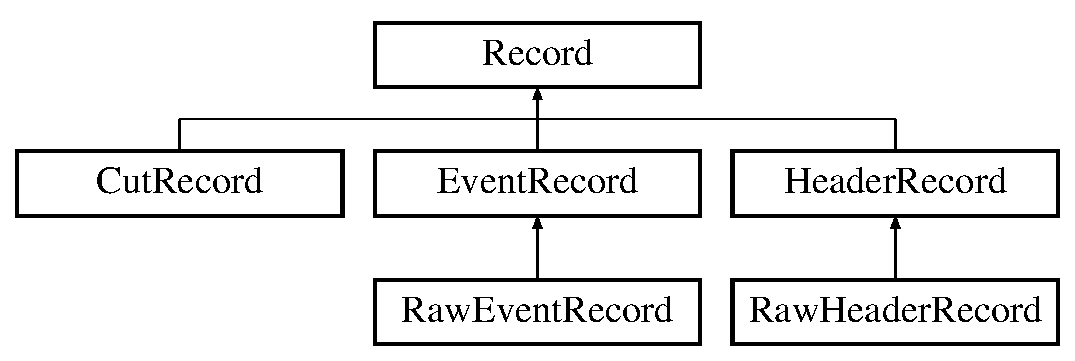
\includegraphics[height=3.000000cm]{structRecord}
\end{center}
\end{figure}


\subsubsection{Detailed Description}
Records are readable/writable (i.e. 

serializable) representations of data. For example, a \hyperlink{classDataReader}{DataReader} should read data from a file and return a \hyperlink{structRecord}{Record} for each event read; the corresponding \hyperlink{classDataWriter}{DataWriter} would write a \hyperlink{structRecord}{Record} to disk. 

Definition at line 18 of file DataRecords.h.



The documentation for this struct was generated from the following file:\begin{DoxyCompactItemize}
\item 
DataRecords.h\end{DoxyCompactItemize}

\hypertarget{structResults}{
\subsection{Results Struct Reference}
\label{structResults}\index{Results@{Results}}
}


Here We Store The \hyperlink{structResults}{Results} of the Chi-\/Square Fit.  




{\ttfamily \#include $<$Fitter.h$>$}

\subsubsection*{Public Attributes}
\begin{DoxyCompactItemize}
\item 
\hypertarget{structResults_ac58008fea6d5883121699bd03afc9ad0}{
double {\bfseries chiSquare}}
\label{structResults_ac58008fea6d5883121699bd03afc9ad0}

\item 
\hypertarget{structResults_ad63d6c2e0ac07d46d691690612a9f8cb}{
int {\bfseries dof}}
\label{structResults_ad63d6c2e0ac07d46d691690612a9f8cb}

\item 
\hypertarget{structResults_a13110d99aaa161562f4e27e2cfe2df21}{
double {\bfseries n0}}
\label{structResults_a13110d99aaa161562f4e27e2cfe2df21}

\item 
\hypertarget{structResults_aa394673cc90385bb560b72f2f024d35c}{
double {\bfseries n0P}}
\label{structResults_aa394673cc90385bb560b72f2f024d35c}

\item 
\hypertarget{structResults_ad28ddcade55d8d6d9b268fb471f04abf}{
double {\bfseries n0M}}
\label{structResults_ad28ddcade55d8d6d9b268fb471f04abf}

\item 
\hypertarget{structResults_a705449c1fc0884235f0c754ed5cd2819}{
double {\bfseries gamma0}}
\label{structResults_a705449c1fc0884235f0c754ed5cd2819}

\item 
\hypertarget{structResults_a15ce9df52af7605eb16df02aef9aa4f0}{
double {\bfseries gammaP}}
\label{structResults_a15ce9df52af7605eb16df02aef9aa4f0}

\item 
\hypertarget{structResults_a95a3bc14352074c0e92455d497ce2069}{
double {\bfseries gammaM}}
\label{structResults_a95a3bc14352074c0e92455d497ce2069}

\item 
\hypertarget{structResults_a44f8bd621620d8e8bd52cc39e188bb01}{
double {\bfseries e0}}
\label{structResults_a44f8bd621620d8e8bd52cc39e188bb01}

\item 
\hypertarget{structResults_a4e532a1c2d1f7b0e229f50dfcc1a8a69}{
double {\bfseries e0P}}
\label{structResults_a4e532a1c2d1f7b0e229f50dfcc1a8a69}

\item 
\hypertarget{structResults_a517afd3bd09e446bc3323bd4a4142d6b}{
double {\bfseries e0M}}
\label{structResults_a517afd3bd09e446bc3323bd4a4142d6b}

\end{DoxyCompactItemize}


\subsubsection{Detailed Description}
Here We Store The \hyperlink{structResults}{Results} of the Chi-\/Square Fit. 

Definition at line 67 of file Fitter.h.



The documentation for this struct was generated from the following files:\begin{DoxyCompactItemize}
\item 
Fitter.h\item 
FitterNew.h\end{DoxyCompactItemize}

\hypertarget{classRunInfo}{
\subsection{RunInfo Class Reference}
\label{classRunInfo}\index{RunInfo@{RunInfo}}
}


Basic structure returned by a \hyperlink{classConfig}{Config} object.  




{\ttfamily \#include $<$Config.h$>$}

Inheritance diagram for RunInfo:\begin{figure}[H]
\begin{center}
\leavevmode
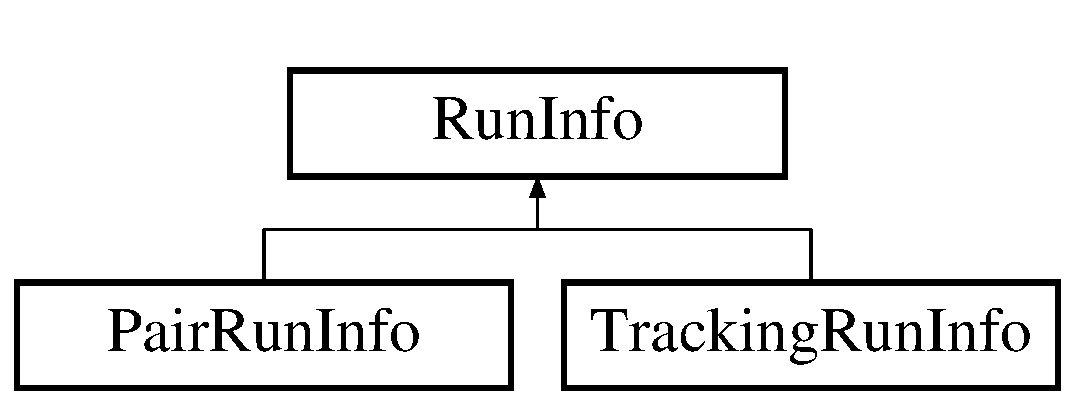
\includegraphics[height=2.000000cm]{classRunInfo}
\end{center}
\end{figure}
\subsubsection*{Public Attributes}
\begin{DoxyCompactItemize}
\item 
\hypertarget{classRunInfo_aaf1aeb4420afcc27e4b1bbd684329fc5}{
char \hyperlink{classRunInfo_aaf1aeb4420afcc27e4b1bbd684329fc5}{type}}
\label{classRunInfo_aaf1aeb4420afcc27e4b1bbd684329fc5}

\item 
\hypertarget{classRunInfo_a8d6402ea556877dfae2b7b28c39a61bf}{
string \hyperlink{classRunInfo_a8d6402ea556877dfae2b7b28c39a61bf}{datadir}}
\label{classRunInfo_a8d6402ea556877dfae2b7b28c39a61bf}

\item 
\hypertarget{classRunInfo_ae87a6169dbd7e2cf46acb700179410bc}{
string \hyperlink{classRunInfo_ae87a6169dbd7e2cf46acb700179410bc}{cachedir}}
\label{classRunInfo_ae87a6169dbd7e2cf46acb700179410bc}

\item 
\hypertarget{classRunInfo_a3910f7bc30936f0f0a5ffa5c46e74ca7}{
string \hyperlink{classRunInfo_a3910f7bc30936f0f0a5ffa5c46e74ca7}{sourcename}}
\label{classRunInfo_a3910f7bc30936f0f0a5ffa5c46e74ca7}

\item 
\hypertarget{classRunInfo_a75fe835214afa525cc0a5bced31cbe57}{
string \hyperlink{classRunInfo_a75fe835214afa525cc0a5bced31cbe57}{onid}}
\label{classRunInfo_a75fe835214afa525cc0a5bced31cbe57}

\item 
\hypertarget{classRunInfo_adc491683f873f002dcfa423f6d0f5bb2}{
string \hyperlink{classRunInfo_adc491683f873f002dcfa423f6d0f5bb2}{offid}}
\label{classRunInfo_adc491683f873f002dcfa423f6d0f5bb2}

\item 
\hypertarget{classRunInfo_a4ed3be46e78ed8c602635ea1397d43e5}{
string \hyperlink{classRunInfo_a4ed3be46e78ed8c602635ea1397d43e5}{n2id}}
\label{classRunInfo_a4ed3be46e78ed8c602635ea1397d43e5}

\item 
\hypertarget{classRunInfo_a01b54d7d93bb39aa3eefaf1bc80e82c2}{
string \hyperlink{classRunInfo_a01b54d7d93bb39aa3eefaf1bc80e82c2}{utdate}}
\label{classRunInfo_a01b54d7d93bb39aa3eefaf1bc80e82c2}

\item 
\hypertarget{classRunInfo_a90970312ece33b627b1f3aee3776b61b}{
string \hyperlink{classRunInfo_a90970312ece33b627b1f3aee3776b61b}{arrayconfig}}
\label{classRunInfo_a90970312ece33b627b1f3aee3776b61b}

\item 
\hypertarget{classRunInfo_ad1332c18766a891c9e94cacb70c0a634}{
double \hyperlink{classRunInfo_ad1332c18766a891c9e94cacb70c0a634}{ra}}
\label{classRunInfo_ad1332c18766a891c9e94cacb70c0a634}

\item 
\hypertarget{classRunInfo_a8540d80a23f779c35c2d55b569562f65}{
double \hyperlink{classRunInfo_a8540d80a23f779c35c2d55b569562f65}{dec}}
\label{classRunInfo_a8540d80a23f779c35c2d55b569562f65}

\item 
\hypertarget{classRunInfo_aaedba21055cfa1183b97a37db043962e}{
double \hyperlink{classRunInfo_aaedba21055cfa1183b97a37db043962e}{zenithoverride}}
\label{classRunInfo_aaedba21055cfa1183b97a37db043962e}

\item 
\hypertarget{classRunInfo_a80bc9fd9b345c07cad754210d744eb4e}{
int \hyperlink{classRunInfo_a80bc9fd9b345c07cad754210d744eb4e}{ntubes}}
\label{classRunInfo_a80bc9fd9b345c07cad754210d744eb4e}

\item 
\hypertarget{classRunInfo_ac25ba9471cf4ddbf4e48c8ec9646ece2}{
double \hyperlink{classRunInfo_ac25ba9471cf4ddbf4e48c8ec9646ece2}{picthresh}}
\label{classRunInfo_ac25ba9471cf4ddbf4e48c8ec9646ece2}

\item 
\hypertarget{classRunInfo_a225661a33c3efe5332083a9372be66a4}{
double \hyperlink{classRunInfo_a225661a33c3efe5332083a9372be66a4}{bndthresh}}
\label{classRunInfo_a225661a33c3efe5332083a9372be66a4}

\item 
\hypertarget{classRunInfo_a3b3285030501c689d84a3dd6d04feaa0}{
double \hyperlink{classRunInfo_a3b3285030501c689d84a3dd6d04feaa0}{padlevel}}
\label{classRunInfo_a3b3285030501c689d84a3dd6d04feaa0}

\item 
\hypertarget{classRunInfo_aeb35b4e6d3a94d92e1092bb3dcd9dea5}{
double \hyperlink{classRunInfo_aeb35b4e6d3a94d92e1092bb3dcd9dea5}{utbase}}
\label{classRunInfo_aeb35b4e6d3a94d92e1092bb3dcd9dea5}

\item 
\hypertarget{classRunInfo_a169dac601c7f6f1be162e95faf0aa83a}{
bool \hyperlink{classRunInfo_a169dac601c7f6f1be162e95faf0aa83a}{padding}}
\label{classRunInfo_a169dac601c7f6f1be162e95faf0aa83a}

\item 
\hypertarget{classRunInfo_a2fb22fc388c3892c01a9939d5034420b}{
bool \hyperlink{classRunInfo_a2fb22fc388c3892c01a9939d5034420b}{pad\_\-track\_\-with\_\-run}}
\label{classRunInfo_a2fb22fc388c3892c01a9939d5034420b}

\item 
\hypertarget{classRunInfo_a16057cde5b36b7c77e7ea7549049e540}{
bool \hyperlink{classRunInfo_a16057cde5b36b7c77e7ea7549049e540}{derotation}}
\label{classRunInfo_a16057cde5b36b7c77e7ea7549049e540}

\item 
\hypertarget{classRunInfo_a4bdb5240f8897d53b71ea7bb1beb1393}{
bool \hyperlink{classRunInfo_a4bdb5240f8897d53b71ea7bb1beb1393}{muoncalibrate}}
\label{classRunInfo_a4bdb5240f8897d53b71ea7bb1beb1393}

\item 
\hypertarget{classRunInfo_ab14a9c15485b7aa14bd5aa99f88d2dcf}{
int \hyperlink{classRunInfo_ab14a9c15485b7aa14bd5aa99f88d2dcf}{outtype}}
\label{classRunInfo_ab14a9c15485b7aa14bd5aa99f88d2dcf}

\item 
\hypertarget{classRunInfo_ae9dfa75fa8232187d96bb0e66d57b963}{
\hyperlink{structCutInfo}{CutInfo} \hyperlink{classRunInfo_ae9dfa75fa8232187d96bb0e66d57b963}{cuts}}
\label{classRunInfo_ae9dfa75fa8232187d96bb0e66d57b963}

\item 
\hypertarget{classRunInfo_af43ac9575e4f5ad74d345b7b7e1a203f}{
double \hyperlink{classRunInfo_af43ac9575e4f5ad74d345b7b7e1a203f}{muon\_\-threshold}}
\label{classRunInfo_af43ac9575e4f5ad74d345b7b7e1a203f}

\item 
\hypertarget{classRunInfo_a76e099c22c2606ef38ebdda51de2c9f0}{
int \hyperlink{classRunInfo_a76e099c22c2606ef38ebdda51de2c9f0}{cuttype}}
\label{classRunInfo_a76e099c22c2606ef38ebdda51de2c9f0}

\item 
\hypertarget{classRunInfo_a045650e484f8e7c8f0832ae48ba210e7}{
string \hyperlink{classRunInfo_a045650e484f8e7c8f0832ae48ba210e7}{mcdatabase}}
\label{classRunInfo_a045650e484f8e7c8f0832ae48ba210e7}

\item 
\hypertarget{classRunInfo_aa3f203cedd871f66e11ca1c341820552}{
string \hyperlink{classRunInfo_aa3f203cedd871f66e11ca1c341820552}{energyestimator}}
\label{classRunInfo_aa3f203cedd871f66e11ca1c341820552}

\item 
\hypertarget{classRunInfo_a4220da66f41648dd38f7442473460b37}{
double \hyperlink{classRunInfo_a4220da66f41648dd38f7442473460b37}{emin\_\-tev}}
\label{classRunInfo_a4220da66f41648dd38f7442473460b37}

\item 
\hypertarget{classRunInfo_ab8e99cca3448bbacecfd25b04d9eb963}{
double \hyperlink{classRunInfo_ab8e99cca3448bbacecfd25b04d9eb963}{emax\_\-tev}}
\label{classRunInfo_ab8e99cca3448bbacecfd25b04d9eb963}

\item 
\hypertarget{classRunInfo_a52cd0b6ef598ab371dde7e850cde1d71}{
int \hyperlink{classRunInfo_a52cd0b6ef598ab371dde7e850cde1d71}{num\_\-e\_\-bins}}
\label{classRunInfo_a52cd0b6ef598ab371dde7e850cde1d71}

\item 
\hypertarget{classRunInfo_a8b754c6ff0b16fc81132e60fc4ae5e11}{
bool \hyperlink{classRunInfo_a8b754c6ff0b16fc81132e60fc4ae5e11}{tubemask} \mbox{[}1024\mbox{]}}
\label{classRunInfo_a8b754c6ff0b16fc81132e60fc4ae5e11}

\item 
\hypertarget{classRunInfo_afc3b0da63379c3f6cc459774145f6765}{
bool \hyperlink{classRunInfo_afc3b0da63379c3f6cc459774145f6765}{camera\_\-offset\_\-analysis}}
\label{classRunInfo_afc3b0da63379c3f6cc459774145f6765}

\item 
\hypertarget{classRunInfo_a5faf94885011f8b93cb1d8c284c25b7f}{
\hyperlink{structCoordinate__t}{Coordinate\_\-t} {\bfseries camera\_\-offset}}
\label{classRunInfo_a5faf94885011f8b93cb1d8c284c25b7f}

\item 
\hypertarget{classRunInfo_af3cf93adf7936184e2684ca8dcb232d3}{
int \hyperlink{classRunInfo_af3cf93adf7936184e2684ca8dcb232d3}{max\_\-ped\_\-events}}
\label{classRunInfo_af3cf93adf7936184e2684ca8dcb232d3}

\item 
\hypertarget{classRunInfo_a5536266accd3a3aae79224e8db27941d}{
bool \hyperlink{classRunInfo_a5536266accd3a3aae79224e8db27941d}{image\_\-filter}}
\label{classRunInfo_a5536266accd3a3aae79224e8db27941d}

\item 
\hypertarget{classRunInfo_a75082b7b3261dccc40a5ea526c91e68b}{
double \hyperlink{classRunInfo_a75082b7b3261dccc40a5ea526c91e68b}{filter\_\-amount}}
\label{classRunInfo_a75082b7b3261dccc40a5ea526c91e68b}

\item 
\hypertarget{classRunInfo_a399514a56d3e8aa99d8a84778107f3c7}{
int \hyperlink{classRunInfo_a399514a56d3e8aa99d8a84778107f3c7}{filter\_\-subdivide}}
\label{classRunInfo_a399514a56d3e8aa99d8a84778107f3c7}

\item 
\hypertarget{classRunInfo_a6281a9efb704753b56516bd7b3ac300f}{
int \hyperlink{classRunInfo_a6281a9efb704753b56516bd7b3ac300f}{filter\_\-iter}}
\label{classRunInfo_a6281a9efb704753b56516bd7b3ac300f}

\item 
\hypertarget{classRunInfo_a22c87862666b62fe0ef8730b2ccecdc2}{
double \hyperlink{classRunInfo_a22c87862666b62fe0ef8730b2ccecdc2}{filter\_\-smoothness}}
\label{classRunInfo_a22c87862666b62fe0ef8730b2ccecdc2}

\item 
\hypertarget{classRunInfo_abf51037c6f453aa857c6050f1b957a9b}{
double {\bfseries filter\_\-percent}}
\label{classRunInfo_abf51037c6f453aa857c6050f1b957a9b}

\item 
\hypertarget{classRunInfo_a28a6b7962b55bfdf725979206e9c86fe}{
double \hyperlink{classRunInfo_a28a6b7962b55bfdf725979206e9c86fe}{filter\_\-threshold}}
\label{classRunInfo_a28a6b7962b55bfdf725979206e9c86fe}

\end{DoxyCompactItemize}


\subsubsection{Detailed Description}
Basic structure returned by a \hyperlink{classConfig}{Config} object. 

Describes all information about the run that is collected from the configuration file -\/ such as override values and data locations

\begin{Desc}
\item[\hyperlink{todo__todo000002}{Todo}]: Make \hyperlink{classRunInfo}{RunInfo} serializable so it can be sent as an MPI message?\end{Desc}


\begin{Desc}
\item[\hyperlink{todo__todo000003}{Todo}]: Make \hyperlink{classRunInfo}{RunInfo} saveable (i.e. write out a config file containing all the settings. This can be written to each run output dir so you can check what settings were used at the last parameterization. You can then use a \hyperlink{classConfig}{Config} object to parse the saved settings and check if the \hyperlink{classRunInfo}{RunInfo} has changed as a robust check for reparameterizing. Save() load() compare()\end{Desc}


Definition at line 117 of file Config.h.



The documentation for this class was generated from the following file:\begin{DoxyCompactItemize}
\item 
Config.h\end{DoxyCompactItemize}

\hypertarget{structRunStatistics}{
\subsection{RunStatistics Struct Reference}
\label{structRunStatistics}\index{RunStatistics@{RunStatistics}}
}
\subsubsection*{Public Attributes}
\begin{DoxyCompactItemize}
\item 
\hypertarget{structRunStatistics_a53b7459d8b2f6448a0fe07bb22ff7e68}{
double {\bfseries significance}}
\label{structRunStatistics_a53b7459d8b2f6448a0fe07bb22ff7e68}

\item 
\hypertarget{structRunStatistics_a891a5cb43e213259d7ab61fc2a383b05}{
double {\bfseries excess}}
\label{structRunStatistics_a891a5cb43e213259d7ab61fc2a383b05}

\end{DoxyCompactItemize}


\subsubsection{Detailed Description}


Definition at line 20 of file Cutter.h.



The documentation for this struct was generated from the following file:\begin{DoxyCompactItemize}
\item 
Cutter.h\end{DoxyCompactItemize}

\hypertarget{structSimShowerRecord}{
\subsection{SimShowerRecord Struct Reference}
\label{structSimShowerRecord}\index{SimShowerRecord@{SimShowerRecord}}
}
\subsubsection*{Public Attributes}
\begin{DoxyCompactItemize}
\item 
\hypertarget{structSimShowerRecord_a2c6c16be74a12a7bd7e5476b715666ab}{
int {\bfseries event\_\-number}}
\label{structSimShowerRecord_a2c6c16be74a12a7bd7e5476b715666ab}

\item 
\hypertarget{structSimShowerRecord_a8fef1a45bc70f3bd2487efa43150eccd}{
int {\bfseries primary\_\-type}}
\label{structSimShowerRecord_a8fef1a45bc70f3bd2487efa43150eccd}

\item 
\hypertarget{structSimShowerRecord_aadaf1fab5a23b6a4cbed2fe5fa8ec5d8}{
double {\bfseries primary\_\-energy}}
\label{structSimShowerRecord_aadaf1fab5a23b6a4cbed2fe5fa8ec5d8}

\item 
\hypertarget{structSimShowerRecord_a2ead0ed3c8c4ea38c01d4e1dd85e4e14}{
\hyperlink{structCoordinate__t}{Coordinate\_\-t} {\bfseries impact\_\-parameter}}
\label{structSimShowerRecord_a2ead0ed3c8c4ea38c01d4e1dd85e4e14}

\item 
\hypertarget{structSimShowerRecord_a86d1bab066fd47e5fff2932137e9cf5b}{
\hyperlink{structCoordinate__t}{Coordinate\_\-t} {\bfseries direction\_\-cos}}
\label{structSimShowerRecord_a86d1bab066fd47e5fff2932137e9cf5b}

\end{DoxyCompactItemize}


\subsubsection{Detailed Description}


Definition at line 45 of file DataRecords.h.



The documentation for this struct was generated from the following file:\begin{DoxyCompactItemize}
\item 
DataRecords.h\end{DoxyCompactItemize}

\hypertarget{classSpectralCutter}{
\subsection{SpectralCutter Class Reference}
\label{classSpectralCutter}\index{SpectralCutter@{SpectralCutter}}
}


Implements cuts which scale with zenith angle and SIZE, otherwise very similar to SuperCuts.  




{\ttfamily \#include $<$SpectralCutter.h$>$}

Inheritance diagram for SpectralCutter:\begin{figure}[H]
\begin{center}
\leavevmode
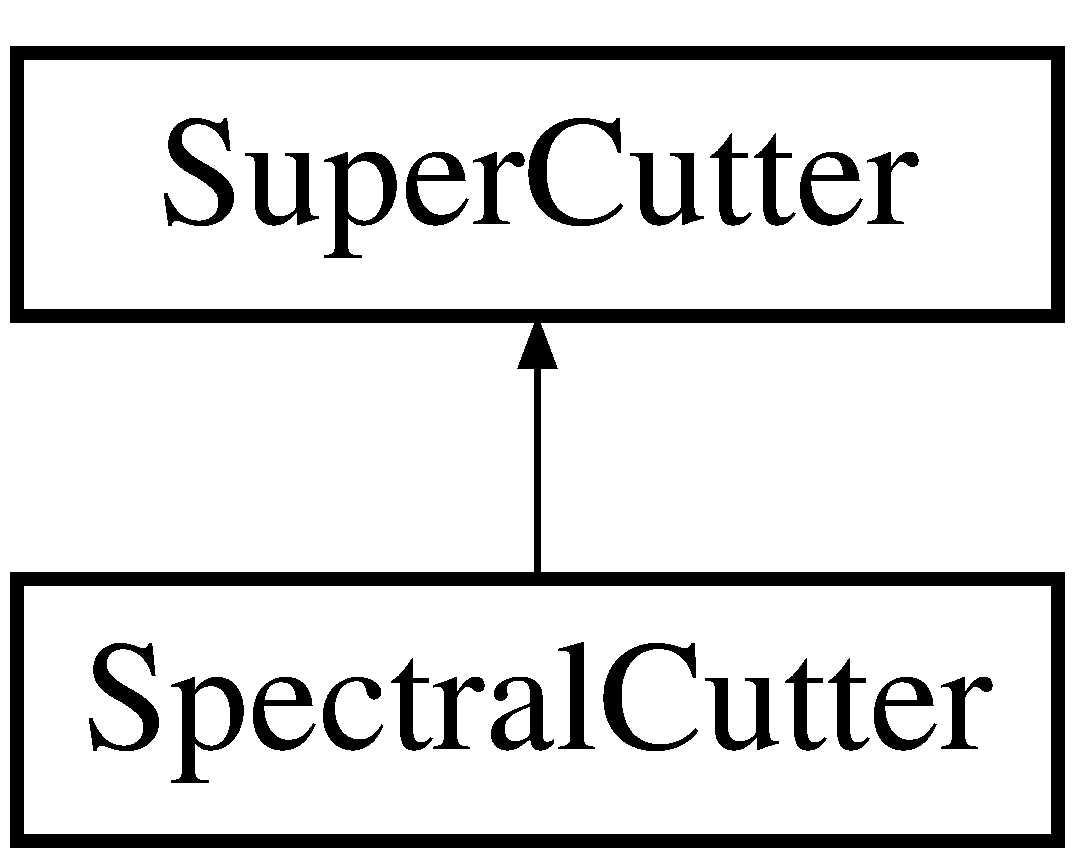
\includegraphics[height=2.000000cm]{classSpectralCutter}
\end{center}
\end{figure}
\subsubsection*{Public Types}
\begin{DoxyCompactItemize}
\item 
enum {\bfseries ParameterEnum} \{ {\bfseries A}, 
{\bfseries B}, 
{\bfseries C}, 
{\bfseries D}
 \}
\end{DoxyCompactItemize}
\subsubsection*{Public Member Functions}
\begin{DoxyCompactItemize}
\item 
\hypertarget{classSpectralCutter_a86026e01fc73d62ba2e8d41816d07a00}{
bool {\bfseries passLength} (\hyperlink{structHillasParameterization}{HillasParameterization} \&param)}
\label{classSpectralCutter_a86026e01fc73d62ba2e8d41816d07a00}

\item 
\hypertarget{classSpectralCutter_a26ee21395280d5cf4ec6ceb6627ae4ad}{
bool {\bfseries passWidth} (\hyperlink{structHillasParameterization}{HillasParameterization} \&param)}
\label{classSpectralCutter_a26ee21395280d5cf4ec6ceb6627ae4ad}

\item 
\hypertarget{classSpectralCutter_ab4ea32e6db4899f1c82daa5ed6b4c9f6}{
double \hyperlink{classSpectralCutter_ab4ea32e6db4899f1c82daa5ed6b4c9f6}{expectedLength} (double size, double zenith)}
\label{classSpectralCutter_ab4ea32e6db4899f1c82daa5ed6b4c9f6}

\item 
\hypertarget{classSpectralCutter_af811b871a1f25c0ca09f8011aa993132}{
double \hyperlink{classSpectralCutter_af811b871a1f25c0ca09f8011aa993132}{modelLength} (double lnsize, const double $\ast$param)}
\label{classSpectralCutter_af811b871a1f25c0ca09f8011aa993132}

\item 
\hypertarget{classSpectralCutter_a841becd5a88abbfd5a942fcaa78ff1ac}{
double \hyperlink{classSpectralCutter_a841becd5a88abbfd5a942fcaa78ff1ac}{expectedWidth} (double size, double zenith)}
\label{classSpectralCutter_a841becd5a88abbfd5a942fcaa78ff1ac}

\item 
\hypertarget{classSpectralCutter_a474e8d284d8e60e13c4edb1be602bc3e}{
double \hyperlink{classSpectralCutter_a474e8d284d8e60e13c4edb1be602bc3e}{modelWidth} (double lnsize, const double $\ast$param)}
\label{classSpectralCutter_a474e8d284d8e60e13c4edb1be602bc3e}

\end{DoxyCompactItemize}


\subsubsection{Detailed Description}
Implements cuts which scale with zenith angle and SIZE, otherwise very similar to SuperCuts. 

Re-\/implements the length and width cuts. 

Definition at line 11 of file SpectralCutter.h.



The documentation for this class was generated from the following files:\begin{DoxyCompactItemize}
\item 
SpectralCutter.h\item 
SpectralCutter.cpp\end{DoxyCompactItemize}

\hypertarget{classStar}{
\subsection{Star Class Reference}
\label{classStar}\index{Star@{Star}}
}


representation of a star  




{\ttfamily \#include $<$StarCatalog.h$>$}

\subsubsection*{Public Attributes}
\begin{DoxyCompactItemize}
\item 
\hypertarget{classStar_ad9ae4846172086e057c241d6a0f21636}{
std::string \hyperlink{classStar_ad9ae4846172086e057c241d6a0f21636}{name}}
\label{classStar_ad9ae4846172086e057c241d6a0f21636}

\item 
\hypertarget{classStar_a4b77ac656e25b91815237dc1899c4199}{
std::string \hyperlink{classStar_a4b77ac656e25b91815237dc1899c4199}{spectclass}}
\label{classStar_a4b77ac656e25b91815237dc1899c4199}

\item 
\hypertarget{classStar_a4e19502f3e68d6ccd8e5fde8d0fe84ac}{
double \hyperlink{classStar_a4e19502f3e68d6ccd8e5fde8d0fe84ac}{ra}}
\label{classStar_a4e19502f3e68d6ccd8e5fde8d0fe84ac}

\item 
\hypertarget{classStar_a69baf3896ff463864dec126ca56a2d58}{
double \hyperlink{classStar_a69baf3896ff463864dec126ca56a2d58}{dec}}
\label{classStar_a69baf3896ff463864dec126ca56a2d58}

\item 
\hypertarget{classStar_a2496dd6541fffff40255753b5981427e}{
double \hyperlink{classStar_a2496dd6541fffff40255753b5981427e}{magnitude}}
\label{classStar_a2496dd6541fffff40255753b5981427e}

\item 
\hypertarget{classStar_a30f20fcd99c18fc89f6d882af59f05c5}{
int \hyperlink{classStar_a30f20fcd99c18fc89f6d882af59f05c5}{epoch}}
\label{classStar_a30f20fcd99c18fc89f6d882af59f05c5}

\item 
\hypertarget{classStar_a91ee659802d043fe26d3538207232975}{
double {\bfseries ora}}
\label{classStar_a91ee659802d043fe26d3538207232975}

\item 
\hypertarget{classStar_a828e0dbc581cd5f9cce51c034d068cf3}{
double \hyperlink{classStar_a828e0dbc581cd5f9cce51c034d068cf3}{odec}}
\label{classStar_a828e0dbc581cd5f9cce51c034d068cf3}

\item 
\hypertarget{classStar_a26184b4582a308b6eb7072b6068b60f1}{
double {\bfseries tx}}
\label{classStar_a26184b4582a308b6eb7072b6068b60f1}

\item 
\hypertarget{classStar_a5e1dedf4e3dc836ef991ce1fb4989041}{
double \hyperlink{classStar_a5e1dedf4e3dc836ef991ce1fb4989041}{ty}}
\label{classStar_a5e1dedf4e3dc836ef991ce1fb4989041}

\item 
\hypertarget{classStar_a2bbf34d3244a49d09bdca8ef13c475d8}{
int \hyperlink{classStar_a2bbf34d3244a49d09bdca8ef13c475d8}{catalog\_\-id}}
\label{classStar_a2bbf34d3244a49d09bdca8ef13c475d8}

\end{DoxyCompactItemize}
\subsubsection*{Friends}
\begin{DoxyCompactItemize}
\item 
\hypertarget{classStar_a5f7c099a163e649e9e998c4542622e1e}{
bool {\bfseries operator$<$} (const \hyperlink{classStar}{Star} \&s1, const \hyperlink{classStar}{Star} \&s2)}
\label{classStar_a5f7c099a163e649e9e998c4542622e1e}

\item 
\hypertarget{classStar_af184317c033dec29617a61c59d402f74}{
bool {\bfseries operator$>$} (const \hyperlink{classStar}{Star} \&s1, const \hyperlink{classStar}{Star} \&s2)}
\label{classStar_af184317c033dec29617a61c59d402f74}

\item 
\hypertarget{classStar_a4c897677c011613260249bd26df7b92f}{
bool {\bfseries operator==} (const \hyperlink{classStar}{Star} \&s1, const \hyperlink{classStar}{Star} \&s2)}
\label{classStar_a4c897677c011613260249bd26df7b92f}

\item 
\hypertarget{classStar_acbbd2067f482caccf398284c650c8546}{
bool {\bfseries operator!=} (const \hyperlink{classStar}{Star} \&s1, const \hyperlink{classStar}{Star} \&s2)}
\label{classStar_acbbd2067f482caccf398284c650c8546}

\item 
\hypertarget{classStar_a34d4a34b441566bae46900ccef8d47d5}{
std::ostream \& {\bfseries operator$<$$<$} (std::ostream \&stream, \hyperlink{classStar}{Star} \&s)}
\label{classStar_a34d4a34b441566bae46900ccef8d47d5}

\item 
\hypertarget{classStar_a2e4c669c771d70c3b0318e4c19d0e4a3}{
std::istream \& {\bfseries operator$>$$>$} (std::istream \&stream, \hyperlink{classStar}{Star} \&s)}
\label{classStar_a2e4c669c771d70c3b0318e4c19d0e4a3}

\end{DoxyCompactItemize}


\subsubsection{Detailed Description}
representation of a star 

Definition at line 11 of file StarCatalog.h.



The documentation for this class was generated from the following file:\begin{DoxyCompactItemize}
\item 
StarCatalog.h\end{DoxyCompactItemize}

\hypertarget{classStarCatalog}{
\subsection{StarCatalog Class Reference}
\label{classStarCatalog}\index{StarCatalog@{StarCatalog}}
}


A searchable star database.  




{\ttfamily \#include $<$StarCatalog.h$>$}

\subsubsection*{Public Member Functions}
\begin{DoxyCompactItemize}
\item 
\hypertarget{classStarCatalog_afc99ce9ea8e23dbcaa9ea3871e1c1224}{
\hyperlink{classStarCatalog_afc99ce9ea8e23dbcaa9ea3871e1c1224}{StarCatalog} ()}
\label{classStarCatalog_afc99ce9ea8e23dbcaa9ea3871e1c1224}

\item 
void \hyperlink{classStarCatalog_ab7577c4758796c622071afb6cd9445f3}{load} (std::string stardbfilename)
\item 
void \hyperlink{classStarCatalog_a067a6b3ebbeed3d8c1450cc7092a9f64}{findNearbyStars} (double, double, double, std::list$<$ \hyperlink{classStar}{Star} $>$ \&)
\item 
void \hyperlink{classStarCatalog_a7b487603d9556b01164515e8fb5fddd9}{precessToDate} (int utdate)
\end{DoxyCompactItemize}


\subsubsection{Detailed Description}
A searchable star database. 

Definition at line 42 of file StarCatalog.h.



\subsubsection{Member Function Documentation}
\hypertarget{classStarCatalog_a067a6b3ebbeed3d8c1450cc7092a9f64}{
\index{StarCatalog@{StarCatalog}!findNearbyStars@{findNearbyStars}}
\index{findNearbyStars@{findNearbyStars}!StarCatalog@{StarCatalog}}
\paragraph[{findNearbyStars}]{\setlength{\rightskip}{0pt plus 5cm}void StarCatalog::findNearbyStars (
\begin{DoxyParamCaption}
\item[{double}]{, }
\item[{double}]{, }
\item[{double}]{, }
\item[{std::list$<$ {\bf Star} $>$ \&}]{}
\end{DoxyParamCaption}
)}}
\label{classStarCatalog_a067a6b3ebbeed3d8c1450cc7092a9f64}


Produces a vector of stars that fall within a specified radius of a specified ra+dec coordinate. 

Also figures out the position of each star in tangential cartesian coordinates, relative to the center position for easy plotting.


\begin{DoxyParams}{Parameters}
{\em ra} & right ascension where the camera is pointing \\
\hline
{\em dec} & declination where the camera is pointing \\
\hline
{\em r} & radius (in degrees) around which to look for stars (should be FOV of camera) \\
\hline
{\em nearbystars} & empty vector of Stars which will be filled up with the results\\
\hline
\end{DoxyParams}
\begin{Desc}
\item[\hyperlink{todo__todo000031}{Todo}]: check that this ra and dec from the tracking computer are already precessed, or from j2000 or something. If not already precessed, they need to be. \end{Desc}


Definition at line 136 of file StarCatalog.cpp.



Referenced by Cutter::cut().

\hypertarget{classStarCatalog_ab7577c4758796c622071afb6cd9445f3}{
\index{StarCatalog@{StarCatalog}!load@{load}}
\index{load@{load}!StarCatalog@{StarCatalog}}
\paragraph[{load}]{\setlength{\rightskip}{0pt plus 5cm}void StarCatalog::load (
\begin{DoxyParamCaption}
\item[{std::string}]{stardbfilename}
\end{DoxyParamCaption}
)}}
\label{classStarCatalog_ab7577c4758796c622071afb6cd9445f3}


Load a saved image. 

Load a database of stars from the specified .edb file (such as those included with XEphem. 

Definition at line 238 of file Image2D.cpp.



References Image2D::setCoordinateBox().

\hypertarget{classStarCatalog_a7b487603d9556b01164515e8fb5fddd9}{
\index{StarCatalog@{StarCatalog}!precessToDate@{precessToDate}}
\index{precessToDate@{precessToDate}!StarCatalog@{StarCatalog}}
\paragraph[{precessToDate}]{\setlength{\rightskip}{0pt plus 5cm}void StarCatalog::precessToDate (
\begin{DoxyParamCaption}
\item[{int}]{utdate}
\end{DoxyParamCaption}
)}}
\label{classStarCatalog_a7b487603d9556b01164515e8fb5fddd9}


Precess star catalog to the current epoch. 


\begin{DoxyParams}{Parameters}
{\em utdate} & for example '020506' for May 6, 2002\\
\hline
\end{DoxyParams}
\begin{Desc}
\item[\hyperlink{todo__todo000032}{Todo}]: Should check this -\/ it looks like stars are moving too much over the course of a year or so, so it's possible this is not working exactly right. However, it's pretty close. \end{Desc}


Definition at line 189 of file StarCatalog.cpp.



Referenced by Cutter::cut().



The documentation for this class was generated from the following files:\begin{DoxyCompactItemize}
\item 
StarCatalog.h\item 
Image2D.cpp\item 
StarCatalog.cpp\end{DoxyCompactItemize}

\hypertarget{classSuperCutter}{
\subsection{SuperCutter Class Reference}
\label{classSuperCutter}\index{SuperCutter@{SuperCutter}}
}


Applies SuperCuts to a given \hyperlink{structHillasParameterization}{HillasParameterization}.  




{\ttfamily \#include $<$SuperCutter.h$>$}

Inheritance diagram for SuperCutter:\begin{figure}[H]
\begin{center}
\leavevmode
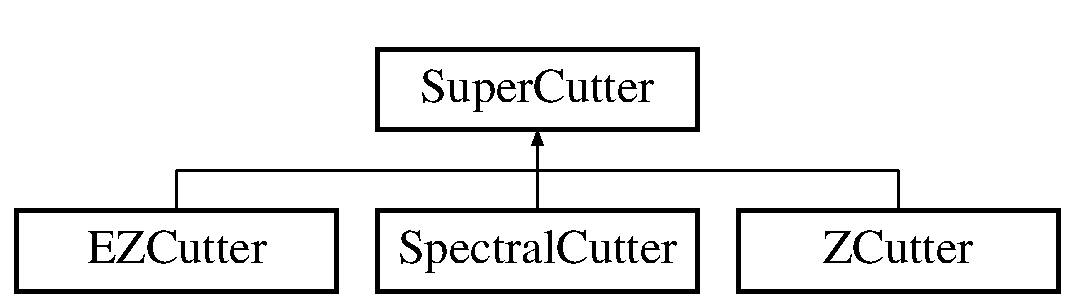
\includegraphics[height=2.000000cm]{classSuperCutter}
\end{center}
\end{figure}
\subsubsection*{Public Member Functions}
\begin{DoxyCompactItemize}
\item 
\hypertarget{classSuperCutter_afef1e5673173418db910fd8b74a0c117}{
void {\bfseries setCuts} (\hyperlink{structCutInfo}{CutInfo} \&cuts)}
\label{classSuperCutter_afef1e5673173418db910fd8b74a0c117}

\item 
virtual void \hyperlink{classSuperCutter_aa9affeb3c4e8b66860f26bd96954b4e1}{applyCorrections} (\hyperlink{structHillasParameterization}{HillasParameterization} \&param)
\item 
bool \hyperlink{classSuperCutter_a10e29b1d569a2b09755e44c31b3c1e61}{pass} (\hyperlink{structHillasParameterization}{HillasParameterization} \&param, int cutmask)
\item 
\hypertarget{classSuperCutter_a2946c8f20d16e08c4f9a8c63b7c237b6}{
virtual bool {\bfseries passSize} (\hyperlink{structHillasParameterization}{HillasParameterization} \&param)}
\label{classSuperCutter_a2946c8f20d16e08c4f9a8c63b7c237b6}

\item 
\hypertarget{classSuperCutter_a0ec9ec3f8df7638aec89c59bf4af458f}{
virtual bool {\bfseries passMax} (\hyperlink{structHillasParameterization}{HillasParameterization} \&param)}
\label{classSuperCutter_a0ec9ec3f8df7638aec89c59bf4af458f}

\item 
\hypertarget{classSuperCutter_ae140b08bee33e70c4df40ff1f48d907e}{
virtual bool {\bfseries passFrac} (\hyperlink{structHillasParameterization}{HillasParameterization} \&param)}
\label{classSuperCutter_ae140b08bee33e70c4df40ff1f48d907e}

\item 
\hypertarget{classSuperCutter_ade36950d2010a1b1aa78920daa7b4eba}{
virtual bool {\bfseries passLensize} (\hyperlink{structHillasParameterization}{HillasParameterization} \&param)}
\label{classSuperCutter_ade36950d2010a1b1aa78920daa7b4eba}

\item 
\hypertarget{classSuperCutter_aa039b048229ae254c2466b6fd0e0a1af}{
virtual bool {\bfseries passLength} (\hyperlink{structHillasParameterization}{HillasParameterization} \&param)}
\label{classSuperCutter_aa039b048229ae254c2466b6fd0e0a1af}

\item 
\hypertarget{classSuperCutter_a2e9282736f529a09555f968edf1f6e60}{
virtual bool {\bfseries passWidth} (\hyperlink{structHillasParameterization}{HillasParameterization} \&param)}
\label{classSuperCutter_a2e9282736f529a09555f968edf1f6e60}

\item 
\hypertarget{classSuperCutter_aab8883f5d3a6933493f423e16c58a92f}{
virtual bool {\bfseries passDistance} (\hyperlink{structHillasParameterization}{HillasParameterization} \&param)}
\label{classSuperCutter_aab8883f5d3a6933493f423e16c58a92f}

\item 
\hypertarget{classSuperCutter_ad44108cabb56ec9f669d228f925bf13e}{
virtual bool {\bfseries passAlpha} (\hyperlink{structHillasParameterization}{HillasParameterization} \&param)}
\label{classSuperCutter_ad44108cabb56ec9f669d228f925bf13e}

\item 
\hypertarget{classSuperCutter_ae32c936000ba52690c06cb47a2bed21a}{
virtual bool {\bfseries passAsymm} (\hyperlink{structHillasParameterization}{HillasParameterization} \&param)}
\label{classSuperCutter_ae32c936000ba52690c06cb47a2bed21a}

\end{DoxyCompactItemize}
\subsubsection*{Protected Attributes}
\begin{DoxyCompactItemize}
\item 
\hypertarget{classSuperCutter_acd3acee447bab464b3a28fca78f08bab}{
\hyperlink{structCutInfo}{CutInfo} {\bfseries \_\-cuts}}
\label{classSuperCutter_acd3acee447bab464b3a28fca78f08bab}

\end{DoxyCompactItemize}


\subsubsection{Detailed Description}
Applies SuperCuts to a given \hyperlink{structHillasParameterization}{HillasParameterization}. 

To use, first call setCuts() to supply the cuts to use, then you can check if an event passed by calling the \hyperlink{classSuperCutter_a10e29b1d569a2b09755e44c31b3c1e61}{pass()} function with appropriate mask (ALL\_\-CUTS will apply all cuts, or you can choose a list of cuts such as SIZE$|$FRAC$|$MAX$|$DISTANCE. 

Definition at line 50 of file SuperCutter.h.



\subsubsection{Member Function Documentation}
\hypertarget{classSuperCutter_aa9affeb3c4e8b66860f26bd96954b4e1}{
\index{SuperCutter@{SuperCutter}!applyCorrections@{applyCorrections}}
\index{applyCorrections@{applyCorrections}!SuperCutter@{SuperCutter}}
\paragraph[{applyCorrections}]{\setlength{\rightskip}{0pt plus 5cm}void SuperCutter::applyCorrections (
\begin{DoxyParamCaption}
\item[{{\bf HillasParameterization} \&}]{param}
\end{DoxyParamCaption}
)\hspace{0.3cm}{\ttfamily  \mbox{[}virtual\mbox{]}}}}
\label{classSuperCutter_aa9affeb3c4e8b66860f26bd96954b4e1}


Apply a filter to the parameters. 

Should always be run before the actual cutting occurs. Modifies param. 

Reimplemented in \hyperlink{classEZCutter_adfef095f257966676350821591df66ed}{EZCutter}, and \hyperlink{classZCutter_ad8fc95579fc4b47a518b66e6ea029f61}{ZCutter}.



Definition at line 87 of file SuperCutter.cpp.



References HillasParameterization::centroid, CutInfo::elongation, HillasParameterization::point\_\-of\_\-origin\_\-a, HillasParameterization::point\_\-of\_\-origin\_\-b, Coordinate\_\-t::x, and Coordinate\_\-t::y.



Referenced by Cutter::cut().

\hypertarget{classSuperCutter_a10e29b1d569a2b09755e44c31b3c1e61}{
\index{SuperCutter@{SuperCutter}!pass@{pass}}
\index{pass@{pass}!SuperCutter@{SuperCutter}}
\paragraph[{pass}]{\setlength{\rightskip}{0pt plus 5cm}bool SuperCutter::pass (
\begin{DoxyParamCaption}
\item[{{\bf HillasParameterization} \&}]{param, }
\item[{int}]{cutmask}
\end{DoxyParamCaption}
)}}
\label{classSuperCutter_a10e29b1d569a2b09755e44c31b3c1e61}


Checks the parameterization of an event to see if it passes cuts. 

Subclasses of this can override the protected methods to re-\/implement different cut types. Also, the prePass() and postPass() functions can be re-\/implemented to allow for special manipulations. As a rule, no \hyperlink{classSuperCutter}{SuperCutter} shuold modify the passed in parameters (even though they are passed by reference, which is done for speed).


\begin{DoxyParams}{Parameters}
{\em param} & set of hillas parameters to check \\
\hline
{\em cutmask} & bitmask of Cuts::CutMask values \\
\hline
\end{DoxyParams}
\begin{DoxyReturn}{Returns}
true if param passwd all cuts specified in cutmast.
\end{DoxyReturn}
\begin{Desc}
\item[\hyperlink{todo__todo000033}{Todo}]: right now, prePass occurs every time a cut is specified. That means it gets redone several times for each event! This shuold be done more efficiently without making it more confusing. \end{Desc}


Definition at line 28 of file SuperCutter.cpp.



References ImageParameterization::invalid.



Referenced by Cutter::cut().



The documentation for this class was generated from the following files:\begin{DoxyCompactItemize}
\item 
SuperCutter.h\item 
SuperCutter.cpp\end{DoxyCompactItemize}

\hypertarget{structSZAEnergyEstimator}{
\subsection{SZAEnergyEstimator Struct Reference}
\label{structSZAEnergyEstimator}\index{SZAEnergyEstimator@{SZAEnergyEstimator}}
}
Inheritance diagram for SZAEnergyEstimator:\begin{figure}[H]
\begin{center}
\leavevmode
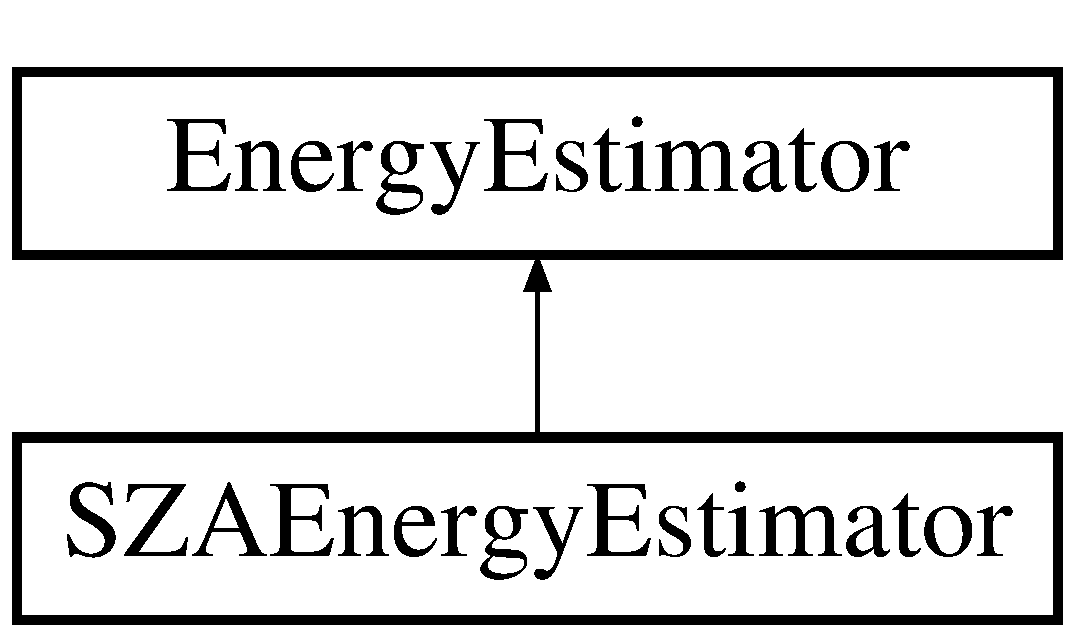
\includegraphics[height=2.000000cm]{structSZAEnergyEstimator}
\end{center}
\end{figure}
\subsubsection*{Public Member Functions}
\begin{DoxyCompactItemize}
\item 
double \hyperlink{structSZAEnergyEstimator_ae1369ba121e67cd939340eee9713ce8b}{getEstimate} (const double size, const double distance, const double zenith=0.366519)
\end{DoxyCompactItemize}


\subsubsection{Detailed Description}


Definition at line 49 of file EnergySpectrum.h.



\subsubsection{Member Function Documentation}
\hypertarget{structSZAEnergyEstimator_ae1369ba121e67cd939340eee9713ce8b}{
\index{SZAEnergyEstimator@{SZAEnergyEstimator}!getEstimate@{getEstimate}}
\index{getEstimate@{getEstimate}!SZAEnergyEstimator@{SZAEnergyEstimator}}
\paragraph[{getEstimate}]{\setlength{\rightskip}{0pt plus 5cm}double SZAEnergyEstimator::getEstimate (
\begin{DoxyParamCaption}
\item[{const double}]{size, }
\item[{const double}]{dist, }
\item[{const double}]{zenith = {\ttfamily 0.366519}}
\end{DoxyParamCaption}
)\hspace{0.3cm}{\ttfamily  \mbox{[}virtual\mbox{]}}}}
\label{structSZAEnergyEstimator_ae1369ba121e67cd939340eee9713ce8b}


Energy estimator for SZA (Z $\sim$= 60 degrees) data. 

This function, which was fit to simulation data, returns the log10 of the estimated energy (log10(EstimatedEnergy)) 

Implements \hyperlink{structEnergyEstimator}{EnergyEstimator}.



Definition at line 80 of file EnergySpectrum.cpp.



The documentation for this struct was generated from the following files:\begin{DoxyCompactItemize}
\item 
EnergySpectrum.h\item 
EnergySpectrum.cpp\end{DoxyCompactItemize}

\hypertarget{classTelescopeArray}{
\subsection{TelescopeArray Class Reference}
\label{classTelescopeArray}\index{TelescopeArray@{TelescopeArray}}
}


Stores information for an array of telescopes, including \hyperlink{classCamera}{Camera} objects.  




{\ttfamily \#include $<$Camera.h$>$}

\subsubsection*{Classes}
\begin{DoxyCompactItemize}
\item 
struct \hyperlink{structTelescopeArray_1_1TelInfo}{TelInfo}
\end{DoxyCompactItemize}
\subsubsection*{Public Member Functions}
\begin{DoxyCompactItemize}
\item 
\hyperlink{classTelescopeArray_ac1cc84c501daa3f8d5ebbdcff8c3e9f8}{TelescopeArray} (std::string filename, std::vector$<$ int $>$ nadc, int utdate)
\item 
\hypertarget{classTelescopeArray_ae26f422cb0497722bbb64e0fd626f9ef}{
int {\bfseries getNumTelescopes} ()}
\label{classTelescopeArray_ae26f422cb0497722bbb64e0fd626f9ef}

\item 
\hypertarget{classTelescopeArray_aa4d1fdecb99be2eae62a9ffb4290980c}{
\hyperlink{classCamera}{Camera} $\ast$ {\bfseries getCamera} (int telescope\_\-id)}
\label{classTelescopeArray_aa4d1fdecb99be2eae62a9ffb4290980c}

\item 
\hypertarget{classTelescopeArray_a817779b9a1bd4aabb28913b20ea65eb5}{
double {\bfseries getLocationX} (int id)}
\label{classTelescopeArray_a817779b9a1bd4aabb28913b20ea65eb5}

\item 
\hypertarget{classTelescopeArray_ab3b41e51f388a0584ea1265a648195c5}{
double {\bfseries getLocationY} (int id)}
\label{classTelescopeArray_ab3b41e51f388a0584ea1265a648195c5}

\item 
\hypertarget{classTelescopeArray_aa36f218df1cf9e4d363fc98f1e6aa818}{
double {\bfseries getLocationZ} (int id)}
\label{classTelescopeArray_aa36f218df1cf9e4d363fc98f1e6aa818}

\item 
\hypertarget{classTelescopeArray_a7e705ecf29d86116ee696f8b39540a9c}{
double {\bfseries getMinX} ()}
\label{classTelescopeArray_a7e705ecf29d86116ee696f8b39540a9c}

\item 
\hypertarget{classTelescopeArray_a10b7f1b976301ede420843c91e6b98cf}{
double {\bfseries getMaxX} ()}
\label{classTelescopeArray_a10b7f1b976301ede420843c91e6b98cf}

\item 
\hypertarget{classTelescopeArray_aac16d5cc1566bde84d43c870b5e892ba}{
double {\bfseries getMinY} ()}
\label{classTelescopeArray_aac16d5cc1566bde84d43c870b5e892ba}

\item 
\hypertarget{classTelescopeArray_adc205ea5f72b1ac2b2c7ac1eab18f671}{
double {\bfseries getMaxY} ()}
\label{classTelescopeArray_adc205ea5f72b1ac2b2c7ac1eab18f671}

\end{DoxyCompactItemize}


\subsubsection{Detailed Description}
Stores information for an array of telescopes, including \hyperlink{classCamera}{Camera} objects. 

Definition at line 92 of file Camera.h.



\subsubsection{Constructor \& Destructor Documentation}
\hypertarget{classTelescopeArray_ac1cc84c501daa3f8d5ebbdcff8c3e9f8}{
\index{TelescopeArray@{TelescopeArray}!TelescopeArray@{TelescopeArray}}
\index{TelescopeArray@{TelescopeArray}!TelescopeArray@{TelescopeArray}}
\paragraph[{TelescopeArray}]{\setlength{\rightskip}{0pt plus 5cm}TelescopeArray::TelescopeArray (
\begin{DoxyParamCaption}
\item[{std::string}]{filename, }
\item[{std::vector$<$ int $>$}]{nadc, }
\item[{int}]{utdate}
\end{DoxyParamCaption}
)}}
\label{classTelescopeArray_ac1cc84c501daa3f8d5ebbdcff8c3e9f8}


Loads an array definition from the specified file and creates a telescope array. 

The array datafile is in the following format:


\begin{DoxyCode}
 WUPARAM-ARRAY-DEFINITION <version number>
 <x location> <y location> <z location> <dish-size> <camera filename> 
 ...
\end{DoxyCode}


for example, 
\begin{DoxyCode}
 WUPARAM-ARRAY-DEFINITION 1.0
 0.0   0.0  0.0  10.0 490.camera
 80.0  0.0  0.0  12.0 veritas-499.camera 
\end{DoxyCode}
 

Definition at line 406 of file Camera.cpp.



References Logger::printf().



The documentation for this class was generated from the following files:\begin{DoxyCompactItemize}
\item 
Camera.h\item 
Camera.cpp\end{DoxyCompactItemize}

\hypertarget{structTelescopeArray_1_1TelInfo}{
\subsection{TelescopeArray::TelInfo Struct Reference}
\label{structTelescopeArray_1_1TelInfo}\index{TelescopeArray::TelInfo@{TelescopeArray::TelInfo}}
}
\subsubsection*{Public Attributes}
\begin{DoxyCompactItemize}
\item 
\hypertarget{structTelescopeArray_1_1TelInfo_a1b871ec4117180cd15d34811b019d1c9}{
double {\bfseries x}}
\label{structTelescopeArray_1_1TelInfo_a1b871ec4117180cd15d34811b019d1c9}

\item 
\hypertarget{structTelescopeArray_1_1TelInfo_ac223c97676242b75e51a8792cddd2848}{
double {\bfseries y}}
\label{structTelescopeArray_1_1TelInfo_ac223c97676242b75e51a8792cddd2848}

\item 
\hypertarget{structTelescopeArray_1_1TelInfo_a342df555ce77431ad16a1dcd7319b3da}{
double {\bfseries z}}
\label{structTelescopeArray_1_1TelInfo_a342df555ce77431ad16a1dcd7319b3da}

\item 
\hypertarget{structTelescopeArray_1_1TelInfo_a171393bb0d26b9ab05d7fb19af625d5e}{
double {\bfseries r}}
\label{structTelescopeArray_1_1TelInfo_a171393bb0d26b9ab05d7fb19af625d5e}

\item 
\hypertarget{structTelescopeArray_1_1TelInfo_a1b0d419406746569f08e9076c748597b}{
\hyperlink{classCamera}{Camera} $\ast$ {\bfseries cam}}
\label{structTelescopeArray_1_1TelInfo_a1b0d419406746569f08e9076c748597b}

\end{DoxyCompactItemize}


\subsubsection{Detailed Description}


Definition at line 96 of file Camera.h.



The documentation for this struct was generated from the following file:\begin{DoxyCompactItemize}
\item 
Camera.h\end{DoxyCompactItemize}

\hypertarget{classThresholdImageCleaner}{
\subsection{ThresholdImageCleaner Class Reference}
\label{classThresholdImageCleaner}\index{ThresholdImageCleaner@{ThresholdImageCleaner}}
}
Inheritance diagram for ThresholdImageCleaner:\begin{figure}[H]
\begin{center}
\leavevmode
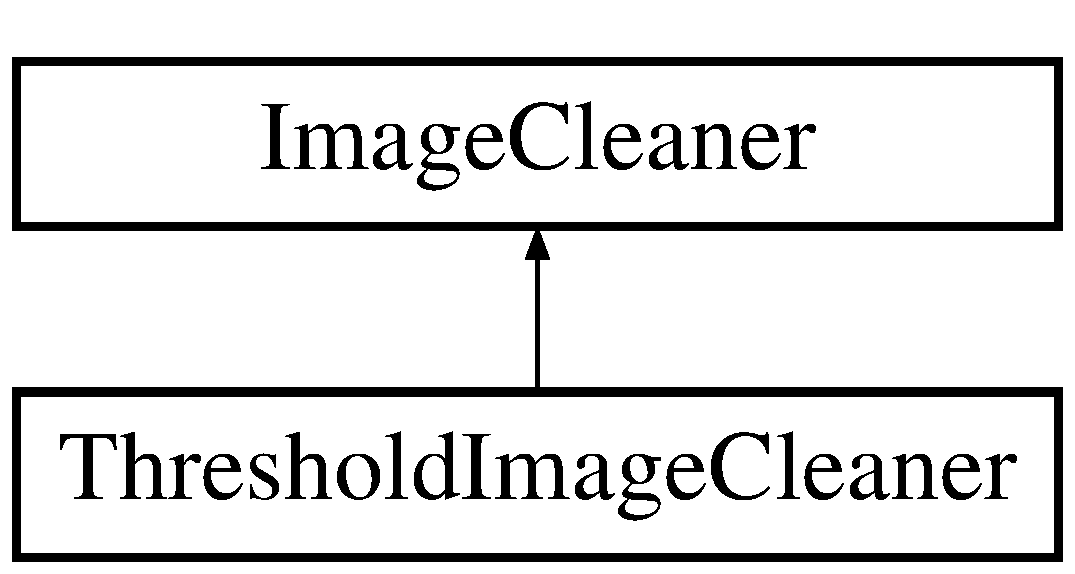
\includegraphics[height=2.000000cm]{classThresholdImageCleaner}
\end{center}
\end{figure}
\subsubsection*{Public Member Functions}
\begin{DoxyCompactItemize}
\item 
\hypertarget{classThresholdImageCleaner_a05c0a4b84a05ac2e4bdf27a7afb953b8}{
{\bfseries ThresholdImageCleaner} (\hyperlink{classCamera}{Camera} \&camera, double threshold)}
\label{classThresholdImageCleaner_a05c0a4b84a05ac2e4bdf27a7afb953b8}

\item 
\hypertarget{classThresholdImageCleaner_a3e13ef3a8c14961f48020090eff22e6f}{
std::vector$<$ int $>$ \& {\bfseries getCleanPixels} (const Array\_\-t \&image)}
\label{classThresholdImageCleaner_a3e13ef3a8c14961f48020090eff22e6f}

\item 
\hypertarget{classThresholdImageCleaner_af24c03f6745f6fa5a818e06c8dc46827}{
void {\bfseries setThreshold} (double t)}
\label{classThresholdImageCleaner_af24c03f6745f6fa5a818e06c8dc46827}

\end{DoxyCompactItemize}


\subsubsection{Detailed Description}


Definition at line 49 of file ImageCleaner.h.



The documentation for this class was generated from the following files:\begin{DoxyCompactItemize}
\item 
ImageCleaner.h\item 
ImageCleaner.cpp\end{DoxyCompactItemize}

\hypertarget{classTrackingRunInfo}{
\subsection{TrackingRunInfo Class Reference}
\label{classTrackingRunInfo}\index{TrackingRunInfo@{TrackingRunInfo}}
}
Inheritance diagram for TrackingRunInfo:\begin{figure}[H]
\begin{center}
\leavevmode
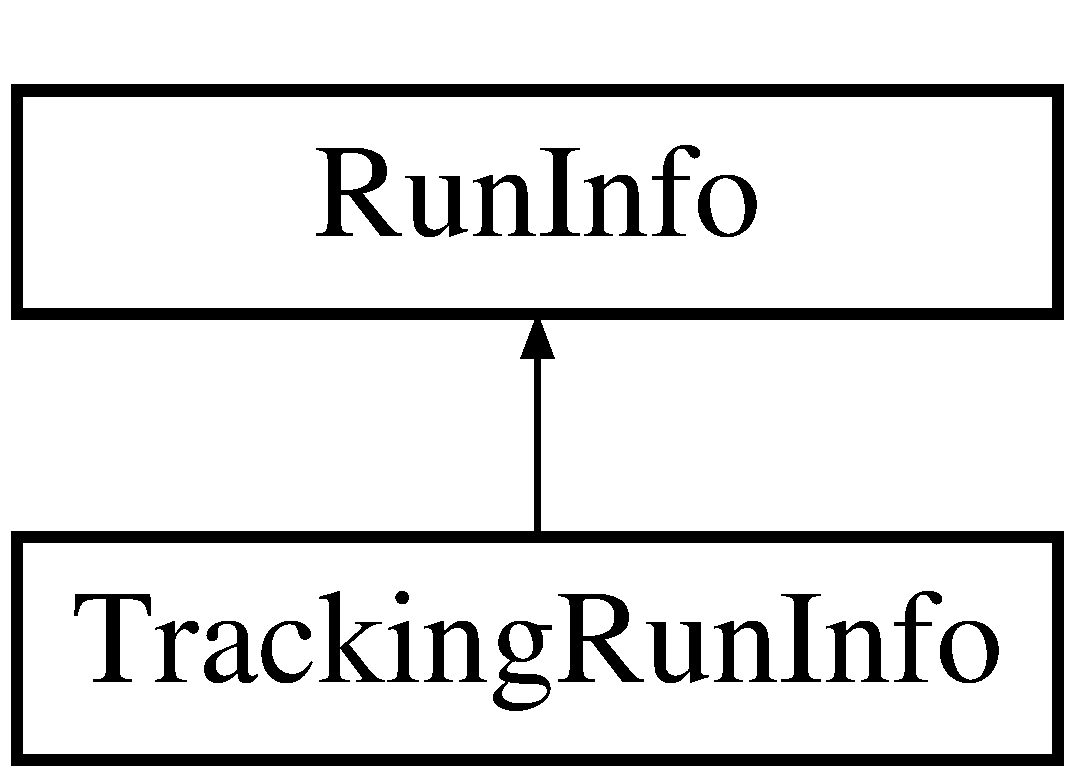
\includegraphics[height=2.000000cm]{classTrackingRunInfo}
\end{center}
\end{figure}


\subsubsection{Detailed Description}


Definition at line 175 of file Config.h.



The documentation for this class was generated from the following file:\begin{DoxyCompactItemize}
\item 
Config.h\end{DoxyCompactItemize}

\hypertarget{structZ40EnergyEstimator}{
\subsection{Z40EnergyEstimator Struct Reference}
\label{structZ40EnergyEstimator}\index{Z40EnergyEstimator@{Z40EnergyEstimator}}
}
Inheritance diagram for Z40EnergyEstimator:\begin{figure}[H]
\begin{center}
\leavevmode
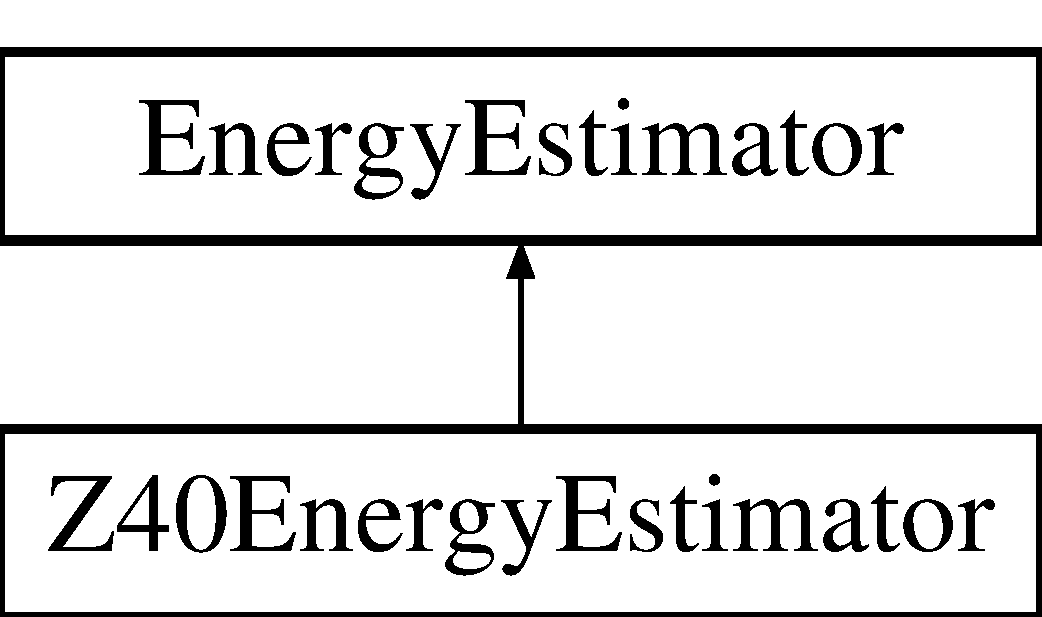
\includegraphics[height=2.000000cm]{structZ40EnergyEstimator}
\end{center}
\end{figure}
\subsubsection*{Public Member Functions}
\begin{DoxyCompactItemize}
\item 
double \hyperlink{structZ40EnergyEstimator_a4b3792f6993cc4cd0cf4e5e4650da1a1}{getEstimate} (const double size, const double distance, const double zenith=0.698131)
\end{DoxyCompactItemize}


\subsubsection{Detailed Description}


Definition at line 54 of file EnergySpectrum.h.



\subsubsection{Member Function Documentation}
\hypertarget{structZ40EnergyEstimator_a4b3792f6993cc4cd0cf4e5e4650da1a1}{
\index{Z40EnergyEstimator@{Z40EnergyEstimator}!getEstimate@{getEstimate}}
\index{getEstimate@{getEstimate}!Z40EnergyEstimator@{Z40EnergyEstimator}}
\paragraph[{getEstimate}]{\setlength{\rightskip}{0pt plus 5cm}double Z40EnergyEstimator::getEstimate (
\begin{DoxyParamCaption}
\item[{const double}]{size, }
\item[{const double}]{dist, }
\item[{const double}]{zenith = {\ttfamily 0.698131}}
\end{DoxyParamCaption}
)\hspace{0.3cm}{\ttfamily  \mbox{[}virtual\mbox{]}}}}
\label{structZ40EnergyEstimator_a4b3792f6993cc4cd0cf4e5e4650da1a1}


Energy estimator for (Z $\sim$= 40 degrees) data. 

This function, which was fit to simulation data, returns the log10 of the estimated energy (log10(EstimatedEnergy)) 

Implements \hyperlink{structEnergyEstimator}{EnergyEstimator}.



Definition at line 162 of file EnergySpectrum.cpp.



The documentation for this struct was generated from the following files:\begin{DoxyCompactItemize}
\item 
EnergySpectrum.h\item 
EnergySpectrum.cpp\end{DoxyCompactItemize}

\hypertarget{structZ50EnergyEstimator}{
\subsection{Z50EnergyEstimator Struct Reference}
\label{structZ50EnergyEstimator}\index{Z50EnergyEstimator@{Z50EnergyEstimator}}
}
Inheritance diagram for Z50EnergyEstimator:\begin{figure}[H]
\begin{center}
\leavevmode
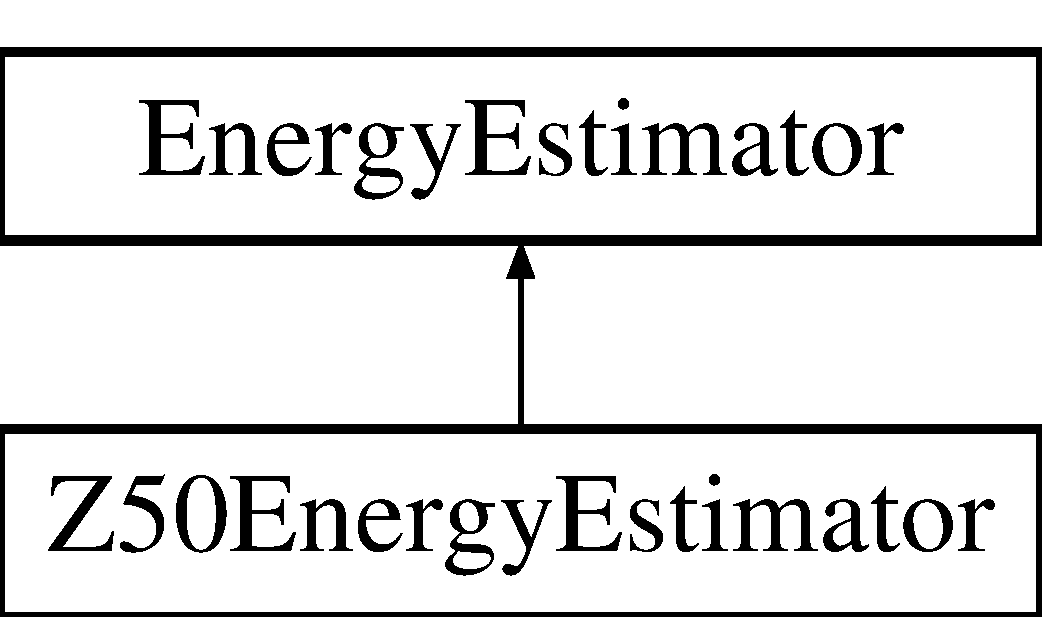
\includegraphics[height=2.000000cm]{structZ50EnergyEstimator}
\end{center}
\end{figure}
\subsubsection*{Public Member Functions}
\begin{DoxyCompactItemize}
\item 
double \hyperlink{structZ50EnergyEstimator_a367c3b5dcfff940f4b54b5622f638da7}{getEstimate} (const double size, const double distance, const double zenith=0.872664)
\end{DoxyCompactItemize}


\subsubsection{Detailed Description}


Definition at line 59 of file EnergySpectrum.h.



\subsubsection{Member Function Documentation}
\hypertarget{structZ50EnergyEstimator_a367c3b5dcfff940f4b54b5622f638da7}{
\index{Z50EnergyEstimator@{Z50EnergyEstimator}!getEstimate@{getEstimate}}
\index{getEstimate@{getEstimate}!Z50EnergyEstimator@{Z50EnergyEstimator}}
\paragraph[{getEstimate}]{\setlength{\rightskip}{0pt plus 5cm}double Z50EnergyEstimator::getEstimate (
\begin{DoxyParamCaption}
\item[{const double}]{size, }
\item[{const double}]{dist, }
\item[{const double}]{zenith = {\ttfamily 0.872664}}
\end{DoxyParamCaption}
)\hspace{0.3cm}{\ttfamily  \mbox{[}virtual\mbox{]}}}}
\label{structZ50EnergyEstimator_a367c3b5dcfff940f4b54b5622f638da7}


Energy estimator for SZA (Z $\sim$= 50 degrees) data. 

This function, which was fit to simulation data, returns the log10 of the estimated energy (log10(EstimatedEnergy)) 

Implements \hyperlink{structEnergyEstimator}{EnergyEstimator}.



Definition at line 227 of file EnergySpectrum.cpp.



The documentation for this struct was generated from the following files:\begin{DoxyCompactItemize}
\item 
EnergySpectrum.h\item 
EnergySpectrum.cpp\end{DoxyCompactItemize}

\hypertarget{classZCutter}{
\subsection{ZCutter Class Reference}
\label{classZCutter}\index{ZCutter@{ZCutter}}
}


Originial zenith cutter, from ZCuts99.  




{\ttfamily \#include $<$ZCutter.h$>$}

Inheritance diagram for ZCutter:\begin{figure}[H]
\begin{center}
\leavevmode
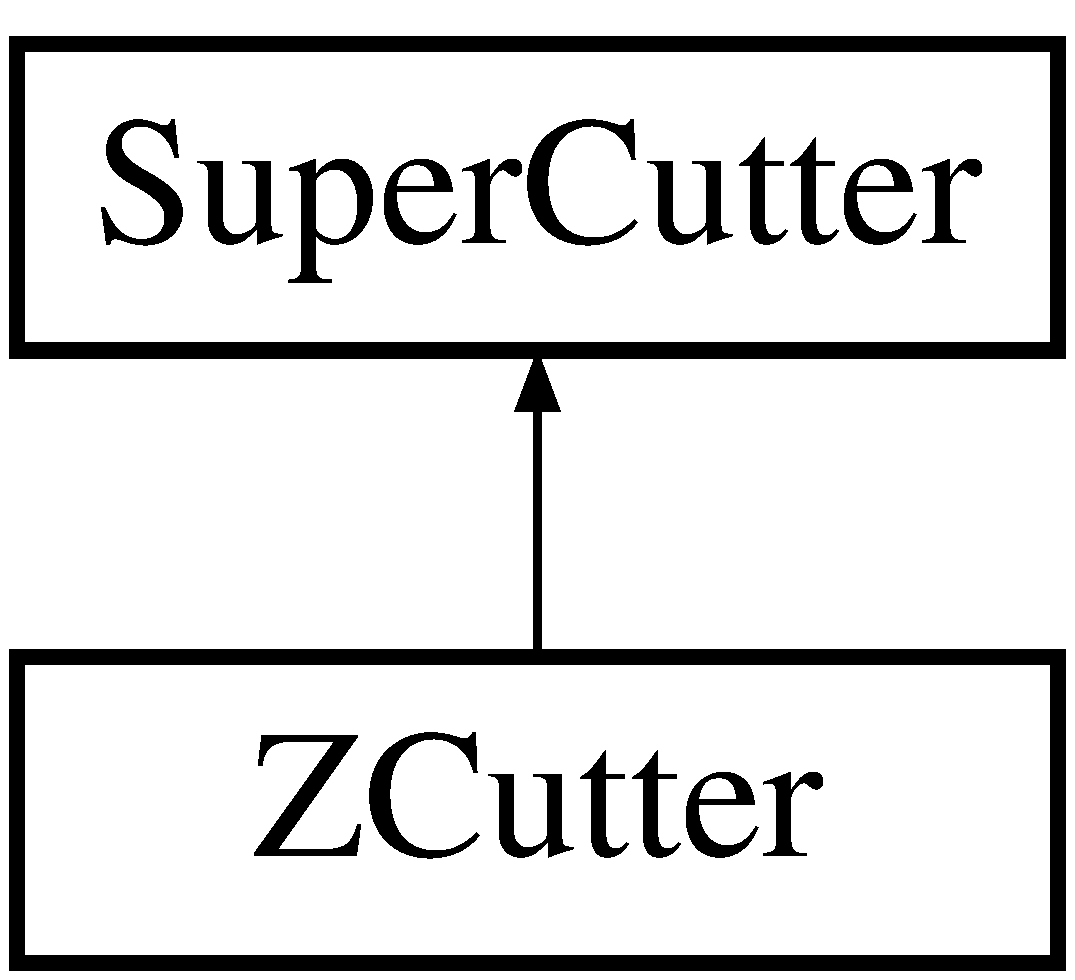
\includegraphics[height=2.000000cm]{classZCutter}
\end{center}
\end{figure}
\subsubsection*{Public Member Functions}
\begin{DoxyCompactItemize}
\item 
void \hyperlink{classZCutter_ad8fc95579fc4b47a518b66e6ea029f61}{applyCorrections} (\hyperlink{structHillasParameterization}{HillasParameterization} \&p)
\item 
\hypertarget{classZCutter_a49d8a4c5de1b717afedb79a2ed00d53e}{
void \hyperlink{classZCutter_a49d8a4c5de1b717afedb79a2ed00d53e}{setCamera} (int npix, int utdate)}
\label{classZCutter_a49d8a4c5de1b717afedb79a2ed00d53e}

\end{DoxyCompactItemize}


\subsubsection{Detailed Description}
Originial zenith cutter, from ZCuts99. 

Uses SuperCuts-\/like cuts, but with zenith angle corrections based on cos(theta). 

Definition at line 12 of file ZCutter.h.



\subsubsection{Member Function Documentation}
\hypertarget{classZCutter_ad8fc95579fc4b47a518b66e6ea029f61}{
\index{ZCutter@{ZCutter}!applyCorrections@{applyCorrections}}
\index{applyCorrections@{applyCorrections}!ZCutter@{ZCutter}}
\paragraph[{applyCorrections}]{\setlength{\rightskip}{0pt plus 5cm}void ZCutter::applyCorrections (
\begin{DoxyParamCaption}
\item[{{\bf HillasParameterization} \&}]{param}
\end{DoxyParamCaption}
)\hspace{0.3cm}{\ttfamily  \mbox{[}virtual\mbox{]}}}}
\label{classZCutter_ad8fc95579fc4b47a518b66e6ea029f61}


Perform zenith correction. 

Overrides the SuperCutter::prePass() function which is executed before cuts are applied by \hyperlink{classSuperCutter_a10e29b1d569a2b09755e44c31b3c1e61}{SuperCutter::pass()}

\begin{Desc}
\item[\hyperlink{todo__todo000035}{Todo}]: make sigma\_\-pix and the \char`\"{}0.023\char`\"{} free optimization parameters! \end{Desc}


Reimplemented from \hyperlink{classSuperCutter_aa9affeb3c4e8b66860f26bd96954b4e1}{SuperCutter}.



Definition at line 40 of file ZCutter.cpp.



References HillasParameterization::centroid, HillasParameterization::distance, CutInfo::elongation, Camera::getPEToDC(), Camera::getSigmaPixel(), Camera::getSigmaPSF(), HillasParameterization::length, HillasParameterization::length\_\-over\_\-size, HillasParameterization::max, HillasParameterization::miss, HillasParameterization::point\_\-of\_\-origin\_\-a, HillasParameterization::point\_\-of\_\-origin\_\-b, HillasParameterization::size, HillasParameterization::width, Coordinate\_\-t::x, Coordinate\_\-t::y, and HillasParameterization::zenith.



The documentation for this class was generated from the following files:\begin{DoxyCompactItemize}
\item 
ZCutter.h\item 
ZCutter.cpp\end{DoxyCompactItemize}

\printindex
\end{document}
